%!TEX root = ../swanton-texts.tex
%%
%% 92. Mountain Dweller (280–288)
%%

\resetexcnt
\chapter{Shaakanaaÿí: Mountain Dweller}\label{ch:92-mountain-dweller}

This narrative was told to \citeauthor{swanton:1909} by \fm{Deikeenaakʼw} John Morris in Sitka in 1904.
In \citeauthor{swanton:1909}’s original publication it is number 92, running from page 280 to 288 and totaling 113 lines of glossed transcription.
The Tlingit name of this story is is \fm{Shaakanaaÿí} which is a posessive noun compound of \fm{shaa} ‘mountain’, \fm{ká} ‘atop’, \fm{naa} ‘clan, nation’, and the possessive noun suffix \fm{-ÿí}.
\fm{Shaakanaaÿí} is the personal name of the mythical figure who is a major character in the second half of the story.
\citeauthor{swanton:1909}’s English title “Mountain Dweller” is an approximation of the Tlingit name.

\citeauthor{swanton:1909} also recorded this story as his number 65 from \fm{Ḵaadashaan} John Katishan in English with the same title of “Mountain Dweller” \parencite[222–224]{swanton:1909}.
Frederica de Laguna recorded it twice in English as “The Story of the Girls who Stole Mountain Goat Tallow” from \fm{Sʼoow Dalé} Minnie Johnson with a comment by \fm{Shaawát Ḵʼwás} Emma Ellis \parencite[892–893]{de-laguna:1972}.
Frances Paul \FIXME{name?} gives a version in English as “Legend of the Mountain Dweller” \parencite[70–71]{paul:1944} which appears to be influenced by \citeauthor{swanton:1909}’s texts but is still distinct with different details.
There is a story about a mythical figure called \fm{Shaatuḵáawu} ‘Man Inside Mountain’ which Catharine McClellan recorded from \fm{Kax̱yéik} Pansy Bailey \parencite[692–695]{mcclellan-cruikshank:2007c} and which Julie Cruikshank recorded from \fm{Ḵʼalgwách} Kitty Smith \parencite[103–107]{smith:1982}, but despite the similar name this story appears to be unrelated to \fm{Shaakanaaÿí}.

\citeauthor{boas:1916} mentions only the two versions of this story recorded by \citeauthor{swanton:1909} in his extensive analysis of narratives in Northwest Coast cultures \parencite[758]{boas:1916}.
He specifically excludes this story from his general grouping of stories involving animals or supernatural beings that marry girls, considering it to be too distinct for his classification.
He also does not mention any stories from other cultures that bear any close resemblance to the \fm{Shaakanaaÿí} story.
\citeauthor{teit:1919} gives the “Story of Cā′kinā” from Tahltan consultants which he says is a version of the \fm{Shaakanaaÿí} story \parencite[244–246]{teit:1919}.
The plot of this narrative has been mixed with the otherwise independent “Beaver and Porcupine” story \parencites[cf.][446–448]{swanton:1908a}[724–727]{boas:1916}[496, 621–622]{mcclellan-cruikshank:2007c}, but the personal name and various details match the Tlingit versions.
\citeauthor{teit:1917} also suggests that the Kaska story “The Fog-Man” \parencite[466–467]{teit:1917} is another version of \fm{Shaakanaaÿí} but it appears to be only tangentially related.

The figure of \fm{Shaakanaaÿí} reportedly appeared in a totem pole in Hoonah which no longer exists.
\citeauthor{swanton:1908} offers a photograph of a model for a pole which was erected for a \fm{Chookaneidí} clan leader called ”Dāx̣ug̣ē′t” which is probably \fm{Daaxoogeit} \parencite[431 fig.\ 109]{swanton:1908}.
He describes this model pole as having \fm{Shaakanaaÿí} at the base surmounted by his dog\footnote{No dog is mentioned in any extant versions of the \fm{Shaakanaaÿí} story.} and an eagle.
According to \citeauthor{swanton:1908}’s consultants, \fm{Shaakanaaÿí} was supposed to be a member of the \fm{Chookaneidí} clan \parencite[432]{swanton:1908}.
\citeauthor{krause:1885} provides a drawing of the original totem pole located in Hoonah, giving much more detail and complexity than the model photographed by \citeauthor{swanton:1909} \parencites[132]{krause:1885}[94]{krause:1956}.
\FIXME{Figure of Krause’s drawing.}
The base of the pole has a dog in the lap of \fm{Shaakanaaÿí} (“schā-kā-nāri”), above whom is an animal labelled “ssāch, Robbe [seal]” that is apparently \fm{sʼaax̱} ‘groundhog’ (a.k.a.\ hoary marmot, \textit{Marmota caligata}).
At the top of the pole is a bird labelled “kī-dschūk, Habicht [hawk]” which is \fm{gijook} \~\ \fm{kijook} (perhaps from \fm{kích} ‘wing’ + \fm{\rt{yuʼk}} ‘shake’).%
\footnote{The exact identity of \fm{gijook} \~\ \fm{kijook} is uncertain but it is some kind of raptor.
Some speakers say it refers to a golden eagle (\textit{Aquila chrysaetos} L.)\ and others to a kind of hawk, i.e.\ \textit{Accipitrinae} or \textit{Buteoninae} \parencites[127]{boas:1917}[257]{krause:1956}[44]{olson:1967}[47]{de-laguna:1972}[28]{naish-story:1976}[33, 255, 441–442, 458]{emmons:1991}[\textsc{m}·137]{leer:2001}.}
\citeauthor{krause:1885} later gives \fm{Shaakanaaÿí} an alternative name “schkā-tā-hīn-āri” \parencites[380]{krause:1885}[251]{krause:1956} which seems to be \fm{Shg̱adaahéen Aaÿí} ‘One of \fm{Shg̱adaahéen}’.
This is likely a reference to \fm{Shg̱adaayi Héen} ‘River that Flows Itself Down’ i.e.\ Waterfall Creek north of Cape Fairweather \parencite[25 \#289, 40 \#31]{thornton:2012}, but the details of the connection are not reported.

In the context of a discussion about cosmology and spirits in his Tlingit ethnography, \citeauthor{swanton:1908} says that \fm{Shaakanaaÿí} is “said to bring good luck to one who hears him chopping and sees where he has been” \parencite[460]{swanton:1908}.
Apparently because of this association with woodworking, \citeauthor{swanton:1908} suggests that \fm{Shaakanaaÿí} may be the same as \fm{Taxgwás} (“Tᴀxgwᴀ′s”) who is “a being who made canoes” that he discusses in a preceding paragraph.
This connection between the two mythical beings seems to be his own speculation, but it is not entirely clear from his writing if this was suggested by his consultants or was his own proposal.
Vanishingly little seems to be recorded about \fm{Taxgwás} besides \citeauthor{swanton:1908}’s mention in this context, the appearance of the name in a song by \fm{Sakwéitʼ} of the \fm{Lʼeeneidí} clan \parencite[410–411 \#82]{swanton:1909}, and a mention by \citeauthor{mcclellan:1975b}.
This latter is repeated here for reference; her \orth{tʼaqwᴀts} implies something like \fm{tʼaḵwáts} but her transcriptions are somewhat unreliable.

\begin{quote}\small
Only the Tagish and Inland Tlingit told of \fm{tʼaqwᴀts}, whom they usually identify as the brother of \fm{tłᴇnax̣idᴀq} [i.e.\ \fm{Tlʼanaxéedáḵw}, see ch.\ \ref{ch:94-wealth-woman}].
He may sometimes be heard chopping away at the top of a tree rather than at the bottom, and the magic chips which fall from his adze bring wealth in the same way that the golden scabs or excrement do, provided again that they are collected and preserved in the proper ritual fashion.
\sourceatright{\parencite[573]{mcclellan:1975b}}
\end{quote}

There is a cassette in the Dauenhauer recordings collection labelled “End of Taxgwas” which is a recording of \fm{Kéet Yanaayí} Willie Marks telling, among other things, the story of \fm{Naatsilanéi} on 26 October 1980 (Dauenhauer recordings collection \#324).
It is unclear if \fm{Naatsilanéi} is in any way connected to \fm{Taxgwás}.
\FIXME{Any further evidence about \fm{Taxgwás}?
And discuss possible connection with \fm{Naatsilanéi} as he is explicitly a carver.}

In his discussion of \fm{Taxgwás} mentioned above, \citeauthor{swanton:1908} claims that the Tlingit figure corresponds to the Haida mythical being of “Wᴀtg̣adagā′ñ” that \citeauthor{swanton:1909} generally labels “Master Carpenter” in English \parencite[30]{swanton:1905b}.
\citeauthor{enrico:2005} gives this name in Skidegate Haida as \fm{7w@t radagaang} [\ipa{ʔwat qatakaːŋ}] and in Masset Haida as \fm{ru ratʼagang} [\ipa{ʔˤu ʔˤatʼakaŋ}], both with unclear meanings \parencite[1623]{enrico:2005}.
Published Haida narratives involving this figure include “Master Carver” \parencite[91]{garfield-forrest:1948}, “How Shining-Heavens caused himself to be born” \parencites[26–31]{swanton:1905b}[284–292]{swanton:1908a}, and “How Master-Carpenter began making a canoe to war with Southeast” \parencite[32–35]{swanton:1905b}.
None of these stories bears any resemblance to the story of \fm{Shaakanaaÿí} so the connection to this Haida figure is tenuous at best.

At least two people have connected the story of \fm{Shaakanaaÿí} to the \fm{Ḵákw Tláa} ‘Basket Mother’ of the \fm{G̱aanax̱teidí} clan in the \fm{Jilḵaat Ḵwáan} \parencites[224]{swanton:1909}[69]{paul:1944}.
This clan possession (\fm{at.óow}) is a large basket often known in English as the “Mother Basket” \parencite[418]{swanton:1908}.
It can be seen below the left housepost in a photograph of the interior of \fm{Yáay Hít} ‘Whale House’ by Winter and Pond in 1885 (fig.\ \ref{fig:92-mountain-dweller-whale-house}).
\citeauthor{emmons:1903} describes this basket in his book \textit{The Basketry of the Tlingit}.

\begin{figure}
\centerfloat
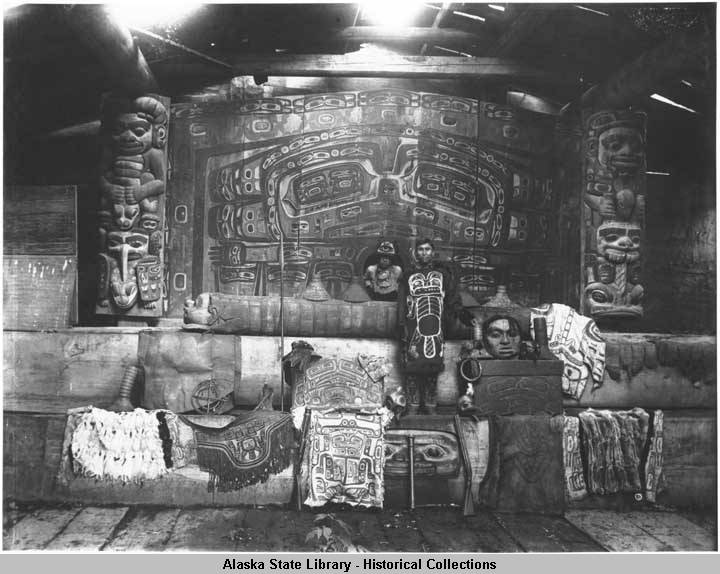
\includegraphics[width=\textwidth, keepaspectratio=true]{figures/ASL-P87-0013-cdmg21_634_full.png}
\caption{Inside \textit{Yáay Hít} ‘Whale House’, Klukwan, 1885 (ASL-P87-0013)}
\label{fig:92-mountain-dweller-whale-house}
\end{figure}

\begin{quote}\small
The most remarkable basket of this type is preserved as an heirloom of the Con-nah-ta-tee clan of the Chilkat tribe, at Klukwan.
It is known as kuhk claw (“basket-mother”) from its great size.
It is cylindrical in form, and measures thirty-three inches [84 cm] both in diameter and in height of walls.
The weave is in khark-ghee-suʼt (No.\ 2), that generally practiced by this people; the only ornamentation consisting of four zigzags at equal intervals, arranged vertically and extending from border to bottom.
It is fitted with four stout, twisted handles of root, by means of which, when filled with food, it is carried into the house and placed before the guests, for only upon occasions of family festivals is this basket ever shown.
It was worked by a woman of the family well back in the last century, but from the care exercised in its preservation it shows but little age.
\sourceatright{\parencite[250–251 fn.\ 1]{emmons:1903}}
\end{quote}

\citeauthor{paul:1944} in her book \textit{Spruce Root Basketry of the Alaska Tlingit} provides another description including details notable to a professional basket weaver.

\begin{quote}\small
Like all Chilkat-woven baskets it was undecorated.
The weaving method was the second technique described ealier in this monograph, alternate rows of weft in double twining and wicker plaiting so that the surface was dull and irregular.
On the outside there were four short, darker lines to mark the capacity at intervals of height, like our commercial measures.
It was fitted with twisted rope handles for transportation.
\sourceatright{\parencite[69]{paul:1944}}
\end{quote}

\citeauthor{swanton:1908} mentions \fm{Ḵákw Tláa} twice in an eyewitness account by \fm{Deikeenaakʼw} John Morris of a \fm{ḵu.éexʼ} (‘inviting people’, i.e.\ potlatch) held by the \fm{G̱aanax̱teidí} clan in Klukwan \parencite[438–442]{swanton:1908}.

\begin{quote}\small
[Host speaking:] “… The people that stay at home (i.e.,\ the Klukwan people) are going to eat out of Mother-basket (kᴀkᵘ ʟa).”
\sourceatright{\parencite[440]{swanton:1908}}
\end{quote}

\begin{quote}\small
After another song, the big basket called Mother-basket was brought out and set before the people of Klukwan. All of the guests ate with horn spoons that had belonged to the dead chief.
\sourceatright{\parencite[441]{swanton:1908}}
\end{quote}

\citeauthor{paul:1944} also describes a \fm{ḵu.éexʼ} in Klukwan in 1901 hosted by the \fm{G̱aanax̱teidí} where \fm{Ḵákw Tláa} was used to carry food to the guests who ere of the \fm{Kaagwaantaan} clan \parencite[69]{paul:1944}.
This seems to be the same \fm{ḵu.éexʼ} described by \fm{Deikeenaakʼw} John Morris given the two \fm{G̱aanax̱teidí} leaders mentioned by name in her account.

\begin{quote}\small
Among these possessions was a huge basket, thirty-three inches in diameter and equally deep, which was placed before the Kok-won-ton guests as their food dish in one of the eating contests, always a feature of potlatches.
\sourceatright{\parencite[69]{paul:1944}}
\end{quote}

\citeauthor{olson:1967} also mentions \fm{Ḵákw Tláa} in a discussion of eating contests during \fm{ḵu.éexʼ}.
Since part of \citeauthor{olson:1967}’s fieldwork was in Klukwan we can presume this information came from one of his \fm{G̱aanax̱teidí} consultants (he was adopted into this clan) during his visits in the 1930s.

\begin{quote}\small
Among the treasures of the Ganaxtedih were a huge basket about three feet high and three in diameter called kŭkTkla (mother of baskets)… The basket held five large boxes of food…
\sourceatright{\parencite[67]{olson:1967}}
\end{quote}

\citeauthor{jones:1914} notes the use of \fm{Ḵákw Tláa} in eating contests as well.
Given that he worked primarily in Juneau, his information probably also comes from people who had personally seen the basket.

\begin{quote}\small
At Kluckwan a chief has in his possession a large basket known as the Mother-of-baskets and a dish (in reality a wooden trough) known as the Worm-dish.
The former stands nearly three feet high from the floor and is about two and one-half feet in diameter…
These two receptacles have been used from time immemorial for eating contests.
They are filled with food, and whichever side eats the contents first wins the contest.
\sourceatright{\parencite[115]{jones:1914}}
\end{quote}

\fm{Ḵaadashaan} John Katishan explicitly connects the story of \fm{Shaakanaaÿí} and the \fm{Ḵákw Tláa} of the \fm{G̱aanax̱teidí} in a short epilogue to his version of this story recorded by \citeauthor{swanton:1909}, as well as mentioning the luck accrued from experiencing \fm{Shaakanaaÿí}’s woodworking activity.

\begin{quote}\small
Nowadays it is a fortunate man that hears Mountain Dweller’s ax or sees where he has been chopping. The basket obtained from him at this time is called Mother-basket (Kᴀkᵘʟa), and is used by the G̣ānᴀxte′dî as an emblem.
\sourceatright{\parencite[224]{swanton:1909}}
\end{quote}

\citeauthor{paul:1944} concurs with this connection in a comment at the end of her version of \fm{Shaakanaaÿí} as well as her presentation of this story in the context of her discussion of \fm{Ḵákw Tláa}.

\begin{quote}\small
Mountain Dweller’s wife kept the miraculous basket and handed it down to her children’s children.
This is the story of their acquisition of the Mother-basket as an emblem, that is told by the Ganak-tady of Chilkat.
\sourceatright{\parencite[71]{paul:1944}}
\end{quote}

This connection between \fm{Ḵákw Tláa} and the baskets in the story of \fm{Shaakanaaÿí} may be reflected in sentences (\ref{ex:92-195-told-mother-baskets}) through (\ref{ex:92-205-put-over-little-finger}).
These describe how, despite the baskets being small enough to fit on \fm{Shaakanaaÿí}’s fingers, they are impossible for all of the men to lift.
This parallels the large size of \fm{Ḵákw Tláa} which needs at least two people to carry it when filled with food.
There is presumably a more general connection to other stories where a basket or box is supernaturally heavy \parencites[236]{swanton:1905}[403–404]{swanton:1908}[466, 888]{boas:1916}[465, 514]{boas:2002}, and this supernatural heaviness can then be further tied to metaphorical interpretations of heaviness and its positive value in Tlingit philosophy \parencite[58–61]{kan:2016}.

\clearpage
\begin{pairs}
\begin{Leftside}
\beginnumbering
% 1
\pstart
\noindent
\snum{1}Ḵuwa.óo áyú yú aanḵáawu, yú aan kulayátʼxʼ.
\snum{2}Áa du ÿátxʼi ḵudzitee.
\snum{3}Dáx̱a̬náx̱ ÿatee du ÿátxʼi.
\snum{4}Du x̱ánde naháaÿi chʼa tlákw us.átch.
\snum{5}G̱una.aan ḵwáani x̱ʼéis át yee akoocháakch yú toow.
\snum{6}Wáa nanée sáyú du x̱ánt uwaḵúx̱ yú yaakw tlein.
\snum{7}Dáḵde wududli.aat.
\snum{8}Yú du léelkʼw jée yéi ÿatee yú toow.
\snum{9}Át ÿee yéi ana.éich g̱una.aan ḵwáani x̱ʼéis.
\snum{10}Tle áyú du dachx̱ánxʼ x̱ʼéix̱ atéex̱ nuch.
\snum{11}Tle yéi ÿanaḵéich yú shaanákʼw
\snum{12}«\!Hé sawáak x̱a\-xʼéesʼch ax̱ jeetx̱ aawayeiḵ.\!»
\pend
% 2
\pstart
\hspace{-0.5em}\snum{13}Aadáx̱ áyú daaḵ awsi.át yú g̱una.aan ḵwáa\-ni.
\snum{14}Aag̱áa ḵaa jikaawaḵaa yú yaneisʼí daa\-kaláḵdi.
\snum{15}Tléikʼ, gwáaÿá l a ÿíkt áa át, yú yaneisʼí.
\snum{16}Yú g̱una.aan ḵwáani ḵwaa áyú ḵéin.
\snum{17}Du jée wuduwajee du yátxʼich yéi wusinei.
\snum{18}A ÿítx̱ ÿawdudzix̱áa.
\snum{19}Hasdu x̱ʼa.eetí sáyú daak kawdudzi.át.
\snum{20}Ách áyú chʼu ÿeedát yéi x̱ʼaÿaduḵáa nuch
\snum{21}«\!Ÿee x̱ʼaÿeetí ÿís daak ḵux̱ dudzi.áat.\!»
\snum{22}Aadáx̱ áyú tléil gwáayú l a ÿíkt áa át.
\snum{23}Aatlein kadéixʼ áyú aawatʼei, yú aanḵáawu.
\snum{24}Aadáx̱ ax̱ʼeiwawóosʼ du ÿátxʼi.
\snum{25}Hasdu sʼíxʼi áyú yax̱ shawdudzix̱áaw.
\snum{26}Chʼa sdu yáx̱ déix̱ ÿatee.
\snum{27}Tlákw hasdu x̱áni yan ool.aatch.
\snum{28}Has\-du tláa hasdu x̱áná̬x̱ daak uwagút.
\snum{29}«\!Ÿeeháanch ágí yéi ÿeeÿsinee?\!»
\snum{30}Tle yéide áyú has gax̱satée áyú tle yetx̱ aÿaa\-washát shátx̱i aa.
\snum{31}Du sée a washtú aka\-dlaakw, tsú kíkʼi aa.
\snum{32}Chʼu dáx̱a̬náx̱ áyú a washtú akaawadlaakw, yú toow yax̱ has aÿawu̬six̱áaÿich áyú, a ÿís daaḵ awsi.ádi aa áyú.
\snum{33}Chʼu tle has woox̱éixʼw.
\snum{34}Taat áyú chʼu tle tʼáa tayee s akaawahaa.
\snum{35}Aadáx̱ ḵu.aa chʼu tle yú shawdudzix̱áawu sʼíxʼ sh eetée yan has awdli.át.
\snum{36}Chʼu tle yú a tʼáak aas tuwóoli, neil has uwa.át.
\pend
% 3
\pstart
\snum{37}Aadáx̱ áyú yéi aÿawsiḵaa
\snum{38}«\!Aadé has na.ádi ÿé óosh gí.\!»
\snum{39}Yéi has adaaÿawsiḵaa
\snum{40}«\!Shaydaḵé déi\!»
\snum{41}Chʼu kuwáatʼ áyú nash\-x̱énch.
\snum{42}Yú sʼíxʼ ásíyú sh eetée yéi s adi.óo.
\snum{43}Hás ḵwa tʼáa kei has ashukawsiháa.
\snum{44}Aadáx̱ áyú anax̱ daaḵ uwagút hasdu tláa.
\snum{45}Tle gwáa\-ÿá l daa át tléil has ḵuwustí.
\snum{46}Aadáx̱ áyú tle daḵdachóon g̱unéi has uwa.át.
\snum{47}Tle g̱unayéi has wu.aadí áwé hasdu eeg̱áa ḵusheeÿí aanáx̱ daaḵ ÿawdig̱ích.
\snum{48}Tle has awdlisín.
\snum{49}Shát\-x̱i aa yéi yandusḵéich, kíkʼi aach
\snum{50}«\!Du ée haa x̱du.aax̱ déi, ax̱ tláa.\!»
\snum{51}Yéi ḵuÿanaḵéich
\snum{52}«\!Haa wáa sás iÿanook i washtú?\!»
\snum{53}Yéi ayanasḵéich du kéekʼ
\snum{54}«\!A yeet x̱á haa ÿaawa\-wóoḵ.
\snum{55}‹\!Shaakanaayéech xʼwán yax̱ ÿee yax̱\-lashaa\!›
\snum{56}yóo x̱á haa daaÿaḵá.
\snum{57}X̱wasikóo ḵu.aa a daa haa daaÿaḵaaÿí.\!»
\pend
% 4
\pstart
\snum{58}Ách áwé tle daḵdachóon g̱unaÿéi has uwa.át.
\snum{59}Chʼa koogéiyi áwé ÿaa s na.át, has gax̱satée nuch.
\snum{60}Ḵúx̱de ash kudanáa du shátx̱, chʼu éiḵdáx̱, du kéekʼ.
\snum{61}Toowúxʼ, hú, tléil ushgú du tláa aÿawuteení.
\snum{62}Wáa yóo s ga.áat sáwé has awsiteen x̱áaw kanax̱ kei ishíxch kag̱áak ÿátkʼw.
\snum{63}Gooch tóode neil uwagút yú kag̱áak.
\snum{64}Aax̱ du kéekʼch yéi ÿawsiḵaa
\snum{65}«\!Kag̱áak Ḵushaanákʼw, leengít ḵutéeni i daa yéi ÿatee.\!»
\snum{66}Yóo ÿaawaḵaa du kéekʼ.
\snum{67}«\!Há leengít x̱á x̱áaw kanax̱ kei x̱at jeewatán\!»
\snum{68}yóo ḵuÿaḵá yú kag̱áak,
\snum{69}«\!‹\!Neildé has g̱ax̱óox̱\!› ax̱ léelkʼw yéi idaayaḵá.\!»
\snum{70}Ách áwé áa yux̱ wujixeex.
\snum{71}Atx̱ áyú héide shuwji\-x̱ein yú x̱ʼaháat.
\snum{72}Has wooḵei.
\snum{73}«\!Daa sá\-kwshí ÿee tushoonáa?\!»
\snum{74}yéi hasdu daaÿaḵá.
\snum{75}Chʼáakw has ḵéini dáx̱ áwé du oox̱ x̱ʼáade at wulitsaaḵ.
\snum{76}Aadáx̱ daaḵ akawlixít.
\snum{77}Atx̱ʼée\-shi kax̱ʼeiltí.
\snum{78}Akaawayúk.
\snum{79}Gán aawatée;
\snum{80}tʼá kíkʼi du oox̱ x̱ʼáadáx̱ át áyú.
\snum{81}A x̱ʼasei\-ÿee aÿawsi.ín tsú, has akʼéetʼ aa.
\snum{82}Kaxwéix̱ du oox̱ x̱ʼáatx̱ daaḵ akawlixít.
\snum{83}Tsu has aawax̱áa.
\snum{84}Yan has at x̱áa áwé tsu yéi aÿawsiḵaa
\snum{85}«\!Daa sá ÿee tushoonáa, ax̱ dachx̱ánxʼi sáani?\!»\hspace*{-0.125ex}
\snum{86}\hspace{-0.125ex}Yóo aÿawsiḵaa
\snum{87}«\!Há Shaakanaayí a yeet haa ÿawduwawóoḵ ax̱ tláach.\!» 
\snum{88}«\!\{L neeÿaaÿi óoshi g̱anix̱ateeyi át\} áwé.
\snum{89}Nay.á dé, ax̱ dachx̱ánxʼi sáani.\!»
\snum{90}Atx̱ áwé ashukaawajaa.
\snum{91}«\!Woochx̱ kʼidag̱át shaa a ÿinaawú, chx̱ánkʼ,
\snum{92}ḵa woochx̱ jida.át sháḵʼw tsú a ÿinaa, chx̱ánkʼ\!»
\snum{93}yóo adaaÿaḵá.
\snum{94}«\!Woochx̱ shát dateet geesh tsú a ÿinaa.
\snum{95}Ÿee lítaÿi xʼwán tsú ÿee jéexʼ, ḵa yaÿéinaa\!»
\snum{96}yéi adaaÿaḵá.
\snum{97}Atx̱ áwé yan ashu\-kaawajáa.
\snum{98}G̱unayéi has uwa.át.
\snum{99}Chʼáakw yaa has na.ádi áwé has awsiteen yú woochx̱ ji\-da.át sháḵʼw.
\snum{100}A x̱ʼéit awsig̱íxʼ sʼaaḵ.
\snum{101}\{Woo\-sh dakádin yóodini\}
\snum{102}Tsu g̱unayéi has uwa\-.át.
\snum{103}\{L kʼát has wu.átch áyú has awsiteen woochx̱ shadag̱át geesh.\}
\snum{104}Sʼíxʼg̱aa a x̱ʼáat has aawag̱íxʼ.
\snum{105}Tle a x̱ʼáanáx̱ has ÿaawa.át.
\snum{106}Atx̱ áyú has awsiteen woochx̱ kʼidag̱át shaa.
\snum{107}(De chʼa aadé kdulneegi ÿé áyá a yáx̱ ÿee een kakwḵalaneek, tlaagú ax̱ daakanóoxʼu.)
\snum{108}Yaÿéinaa a x̱ʼáat has awsig̱íxʼ.
\snum{109}Aanáx̱ has ÿaawa.át.
\snum{110}Has awsiteen yú ḵu.oo.
\snum{111}A hídi yát has uwa.át.
\pend
% 5
\pstart
\snum{112}Du tláa gwáaÿá neil.
\snum{113}A ÿée tléil duteen táaych.
\snum{114}Shaakanaaÿí hídi, a ÿeet has ÿawduwawóoḵ.
\snum{115}Ách áyú has aÿaawadlaaḵ.
\snum{116}Chʼáakw has ḵéini áwé du x̱ʼéix̱ at dutéex̱.
\snum{117}Yaa ndayáan wé at sʼaatí.
\snum{118}Chʼu tle aawa\-wóosʼ du tláa, a x̱ʼaÿíx̱,
\snum{119}«\!Wáa sá ḵoowa\-nook?
\snum{120}Ḵu.oo áwé i x̱ánt has uwa.át.\!»
\snum{121}«\!I ÿeet has ÿawduwawóoḵ yax̱ has ÿag̱eelasháat áhé.\!»
\snum{122}Tle yax̱ aÿawlisháa Shaakanaayích.
\snum{123}Chʼáakw nastée áwé at wooxoon.
\pend
% 6
\pstart
\snum{124}Yéi aÿawsiḵaa du shátxʼi yán
\snum{125}«\!Tléil ooltsáakw yú ax̱ een yéi nateech ḵáa, yú ax̱ tláach.\!»
\snum{126}A yáx̱ áwé ḵáasʼ hasdu jée yéi wootee, hasdu náḵ nagóot.
\snum{127}Chʼu tle yá a ÿeen áa ÿatee áwé galtáa daaḵ aawatée yú at kageidí.
\snum{128}Yanax̱ aawatsaaḵ.
\snum{129}Át akaawagán.
\snum{130}De chʼa ách ḵusa.een át áyú, du ÿéet shátxʼi ÿán.
\snum{131}Átx̱ áwé chʼu tle has aji.ín.
\snum{132}Adaakaawagaan.
\snum{133}Du ÿéet shátxʼi ÿán kaadé áwé kei ashakawlitáḵ.
\snum{134}Tle yú ḵáasʼch a ÿinaadé kei has akawlixít.
\snum{135}Has aawajáḵ hasdu chaan.
\snum{136}Gáani yux̱ has aawa\-x̱óotʼ.
\snum{137}A kát has ḵushakaawaháa.
\snum{138}Chʼa yéi gugéikʼ áwé ḵútlʼkw tóonáx̱ wulishoo.
\pend
% 7
\pstart
\snum{139}Wooyeix̱ du ÿéet.
\snum{140}Haat góot áwé aa\-tlein áyú ÿaa anayáan yú jánwu.
\snum{141}Aawa\-wóosʼ du tláa.
\snum{142}«\!X̱ách aadé keeneek yé x̱á haa wusinee.
\snum{143}Du kaadé áa yax̱ kawtulitáḵ.
\snum{144}Éig̱i yux̱ wutuwax̱óotʼ.\!»
\snum{145}«\!Ÿakʼéi aadé ÿeeÿsineeÿi ÿé\!»
\snum{146}tle yóo aÿawsiḵaa.
\snum{147}«\!Ax̱ tláa, de chʼáakw áwé a x̱áni yéi teex̱ leengít tléil ooltsáakw.\!»
\snum{148}Atx̱ áwé woosh kaadé yéi awsinee yú at kageidí ḵa yú at ÿik.ádi ḵa yú toow sákw.
\pend
% 8
\pstart
\snum{149}Shaakanaaÿí, xʼoon du káa ÿan ḵula.áat sáwé yéi aÿawsiḵaa du shátxʼi ÿán
\snum{150}«\!Tléigíl neil yáx̱ ÿeetaawu.aasch?\!»
\snum{151}«\!Aaá\!» tle yóo has aÿawsiḵaa.
\snum{152}Aan has akaawaneek
\snum{153}«\!A ÿeet haa ÿaawawóoḵ ax̱ tláach.
\snum{154}Ách áyá i kayaadé wutuwa.aat.\!»
\snum{155}«\!Ha ḵákw ÿee.ák.\!»
\snum{156}A yáx̱ áwé has a.áak.
\snum{157}«\!Chʼa ÿee yáx̱, déix̱ xʼwán ÿee góosh náax̱ ÿee.ák.\!»
\snum{158}Wáa nanée sáwé a ÿeedé has aawahaa yú hasdu tlʼeiḵ náax̱ has aawa.ági át.
\snum{159}G̱unayéi has gug̱a.áat.
\snum{160}Xʼoon shaa sáyú a niÿaa.
\snum{161}Áa ÿéi yan kudagáa áwé, yú ḵákw, xʼoon yaakw ÿik.ádi sáyú,
\snum{162}chʼu déix̱ aa áwé du tlʼeiḵ náax̱ daaḵ aÿawli.át.
\snum{163}Chʼu déix̱ aan g̱unéi has uwa.át.
\snum{164}Chʼa xʼoon sáyú has uwax̱éi.
\pend
% 9
\pstart
\snum{165}Aan yaa has na.ádi, chʼa g̱unaÿéide áyú yóo kaaxát.
\snum{166}Yú Shaakanaaÿí tóonáx̱ ax̱di\-gáan.
\snum{167}Wáa nanée sáwé ÿetx̱ kawdiÿáa du éesh aaní.
\snum{168}Aan kulayátʼ.
\snum{169}Xáanaa áwé wé hít ÿát has uwa.át.
\snum{170}Du goosh náax̱ áwé daaḵ aÿawli.át yú ḵákwxʼ sáani.
\snum{171}De chʼa yéi át has toowditán hasdu éekʼáktskʼu hasdu x̱áni yux̱ nag̱asheex.
\snum{172}Has aawax̱oox̱.
\snum{173}De hasdu eetí yan yoo at kaawatée.
\snum{174}De a kát ḵutéen.
\snum{175}Ách áyú tle neildé wujixeex.
\snum{176}Tle du tláa yéi aÿawsiḵaa
\snum{177}«\!Ax̱ dláakʼ gáant has uwa.át.\!»
\snum{178}Tle áwé xʼaandéin adaané, du ÿéet kʼátskʼu, de áa awlixaají, du dláakʼ.
\snum{179}«\!Sh ḵʼawdliyél\!»
\snum{180}yóo adaaÿaḵá.
\snum{181}Chʼa g̱áax̱ kíknáx̱ áwé aadé woogoot.
\snum{182}Tsu neil góot áwé tsu akaneek du tláa tin.
\snum{183}«\!Áwu hás.
\snum{184}Kʼé áa yux̱ nagú.\!»
\snum{185}«\!Hasdu kʼóox lʼeedí haat aa lakʼoots.\!»
\snum{186}Akanéek.
\snum{187}(Dei chʼa aadé tlaagú kadulnik ÿé, a yáx̱ áÿá ÿee een kax̱anéek.)
\snum{188}Neil awlishát.
\snum{189}Cha chʼa aag̱áa áwé tsá aadé wudigoot du tláa.
\snum{190}Áa yux̱ aw\-dlig̱ein.
\snum{191}Xʼéig̱aa du ÿátxʼi gwáaÿá.
\snum{192}«\!Neil ÿee.á\!»
\snum{193}yóo aÿawsiḵaa.
\snum{194}Du x̱áni neil uwa\-.át.
\snum{195}Atx̱ áwé du tláa tin akaawaneek yú \mbox{ḵákwxʼ.}
\snum{196}Yú Shaakanaaÿéech shakaawayóok áwé yú ḵákwxʼ;
\snum{197}«\!Aatlénxʼ áyú gáanu, ḵákw.
\snum{198}Neil g̱adul.aadí\!»
\snum{199}yóo ÿaawaḵaa.
\snum{200}Dáx̱a̬\-náx̱ áyú áa yux̱ aawa.aat.
\snum{201}Tsʼas yan ḵoowa\-xéch.
\snum{202}Tsu áa yux̱ aawagoot.
\snum{203}Ldakát ḵáach áyú neildé has asaÿahéi.
\snum{204}Yan ḵuxéich áyú ḵaa daséixʼán wudihaan yú ḵákwxʼde.
\snum{205}Yan yoo ḵuxéich áyú du wankatlʼeiḵnáx̱ daaḵ aÿawli.át yú ḵákwxʼ, Shaakanaaÿéech.
\snum{206}Áyú gu.aa yú taaÿí, jánwu ÿígi.
\snum{207}A washtú akawudlaagúch áwé, du tláach, du sée hás;
\snum{208}ách áwé tsʼas a taaÿí aa yú aantḵeiní a ÿís wóosht ayaawa.íxʼ.
\snum{209}Yú ḵákwxʼ ka.ádi ldakát ḵáa kaanáx̱ áyú wootee, yú ḵákwxʼ ka.ádi.
\snum{210}Haa leengít aaní ḵákwxʼ áyú.
\pend
\endnumbering
\end{Leftside}
%%
%% Column break.
%%
\begin{Rightside}
\beginnumbering
% 1
\pstart
\noindent
\snum{1}He dwells, that aristocrat, in the length of a town.
\snum{2}His children live there.
\snum{3}They are two, his children.
\snum{4}Travellers always come near him.
\snum{5}For foreigners to eat, he would always store it below things, that tallow.
\snum{6}At some point it came near him, that big canoe.
\snum{7}People brought them inland.
\snum{8}It is in his grandmother’s possession, that tallow.
\snum{9}She always stored it below things for foreigners to eat.
\snum{10}Then she would always give it to her grandchildren.
\snum{11}Then she would say, that little old lady,
\snum{12}\qqk{}“This matted mongrel took it from me.”
\pend
% 2
\pstart
\snum{13}After that he made them come up, those foreigners.
\snum{14}He told people to work on getting it, that box of tallow.
\snum{15}No, apparently there is no thing sitting within it, that tallow.
\snum{16}Those foreigners however are seated.
\snum{17}In his possession they thought that his children had done it.
\snum{18}They ate it all up from inside of it.
\snum{19}Apparently people brought out their leftovers.
\snum{20}That is why even now people always say
\snum{21}They have at last brought it back out for your leftovers.
\snum{22}After that there is apparently no thing sitting with in it.
\snum{23}It was great shame that he found, that aristocrat.
\snum{24}After that he asked his children.
\snum{25}It was their dishes that had been made all hairy.
\snum{26}Just like them there are two.
\snum{27}They always put them down next to them.
\snum{28}Their mother came out near them.
\snum{29}\qqk{}“Is it you who have done this?”
\snum{30}Then them having cried so, she picked up her face, the older sister.
\snum{31}She scratches the inside cheek of her daughter, and her younger sister too.
\snum{32}It was the two of them that she scratched the inside of their cheeks, because they ate up all of that tallow, the stuff that they had put away for them.
\snum{33}Then they slept.
\snum{34}It was at night that they dug it then beneath the boards.
\snum{35}After that however, they had put down those dishes that had been made all hairy in their places.
\snum{36}Then the hole in a tree behind them, they went inside it.
\pend
% 3
\pstart
\snum{37}Later she said to her
\snum{38}\qqk{}“Maybe perhaps it’s the way that they have gone there.”
\snum{39}She said to them
\snum{40}\qqk{}“Get up now!”
\snum{41}It was just the length that would move [as she pulled at the covers].
\snum{42}It is those dishes that they have in their places.
\snum{43}Them however, they dug up the end of the board.
\snum{44}Then she came out through it, their mother.
\snum{45}So apparently they just don’t exist.
\snum{46}Then it was that they started going directly inland.
\snum{47}Then it was when they had started going that they pierced through it searching for them.
\snum{48}Then they hid.
\snum{49}She would say to the elder sister, the younger one
\snum{50}\qqk{}“We should be heard to her now, my mother.”
\snum{51}She would say
\snum{52}“How perhaps do you feel it, the inside of your cheek?”
\snum{53}So she says to her, her younger sister
\snum{54}\qqk{}“They lack confidence in us about it, you know.
\snum{55}\qqk{}‘The Shaakanaayí should marry you all’
\snum{56}so she said about us, you know.
\snum{57}But I know that she says it about us.”
\pend
% 4
\pstart
\snum{58}That is why they started going directly inland.
\snum{59}It is aimlessly that they are going along while always crying.
\snum{60}She keeps telling her to go, her older sister, back from the beach, her younger sister.
\snum{61}To her it was not enjoyable, for her mother to have recognized her.
\snum{62}Them having gone up off somehow, they saw running along the top of a log a tiny deermouse.
\snum{63}It went inside into a hill, that deermouse.
\snum{64}After that her younger sister said to it
\snum{65}\qqk{}“Little Old Deermouse, people’s vision is around you.”
\snum{66}So said her younger sister.
\snum{67}\qqk{}“Well, a person indeed has led me up along the top of a log”
\snum{68}so one says, that deermouse,
\snum{69}\qqk{}“‘Summon them home’ my grandparent says about you.”
\snum{70}That is why it ran outside there.
\snum{71}After that it opened, that door.
\snum{72}They sat.
\snum{73}\qqk{}“What perhaps drives you?”
\snum{74}so it says to them.
\snum{75}After sitting for a long time, she poked something between her teeth.
\snum{76}She picked it out from there.
\snum{77}A dryfish crumb.
\snum{78}She shook it.
\snum{79}She put it in the fire;
\snum{80}king salmon is the thing that she pulled from between her teeth.
\snum{81}Also she put it before them to eat, the stuff that they consume.
\snum{82}She picked a cranberry out from between her teeth.
\snum{83}Again they ate it.
\snum{84}Having finished eating things, again they said to them
\snum{85}\qqk{}“What drives you, my little grandchildren?”
\snum{86}So she says to it
\snum{87}\qqk{}“She lacks confidence in us about the Shaakanaayí, you know, my mother.”
\snum{88}\{“It is a thing very difficult to get near\}
\snum{89}Go now, my little grandchildren.”
\snum{90}After that it instructed her.
\snum{91}\qqk{}“The mountain whose bases fall apart is in its way, little grandchild,
\snum{92}and the \fm{sháḵʼw} that fight with each other also are in its way, little grandchild.”
\snum{93}so it says to her.
\snum{94}\qqk{}“The kelp whose heads are moved against each other by waves also are in its way.
\snum{95}Also be sure your knives are in your possession, and whetstone.”
\snum{96}so it says to her.
\snum{97}After that it was done instructing her.
\snum{98}They started going.
\snum{99}Going along for a long time, they saw the \fm{sháḵʼw} that fight with each other.
\snum{100}She threw at their mouths a bone.
\snum{101}\{They departed together with them.\}
\snum{102}Again they started going.
\snum{103}\{Before they had gone far they came upon kelps floating together.\}
\snum{104}They threw moss between it.
\snum{105}Then they went off along between them.
\snum{106}After that they saw it, that mountain whose bases fall apart.
\snum{107}(Now just the way that they tell it, I will tell it to you like that, my ancient grandparents.)
\snum{108}They threw a whetstone between them.
\snum{109}They went off along through them.
\snum{110}They saw them, the people.
\snum{111}They went to the face of their house.
\pend
% 5
\pstart
\snum{112}Apparently it is his mother here in the house.
\snum{113}Inside of it people cannot see because of the fat.
\snum{114}The Shaakanaaÿí’s house, people lacked confidence in them about it.
\snum{115}That is why they accomplished it.
\snum{116}Sitting for a long time, they repeatedly give them things to eat.
\snum{117}He is packing, the hunter.
\snum{118}Just then he asked her, his mother, in the mouth of it,
\snum{119}\qqk{}“What has happened?
\snum{120}There are people who have come to you.”
\snum{121}\qqk{}“People lacked confidence in them about you, that you should marry them all.”
\snum{122}So then he married them all, the Shaakanaayí.
\pend
% 6
\pstart
\snum{123}A long time having passed, he readied for things.
\snum{124}He said to his wives
\snum{125}\qqk{}“She does not have them last long, people who stay with me, my mother.”
\snum{126}It was like that that they came to have sticks in their possession, him having left them.
\snum{127}Then it is during that time that she put it down in the middle of the fire, a side of meat.
\snum{128}She stuck it into the ground.
\snum{129}It caught on fire there.
\snum{130}Now that is just the thing that she kills people with, her son’s wives.
\snum{131}After that they watch her hands.
\snum{132}Its outside burned.
\snum{133}It was toward her son’s wives that she pushed the top of it.
\snum{134}Then they pushed it up in her direction with those sticks.
\snum{135}They killed her, their mother-in-law.
\snum{136}They dragged her outside.
\snum{137}They covered her over.
\snum{138}It was only a little bit that stuck out through the mud.
\pend
% 7
\pstart
\snum{139}He was gone, her son.
\snum{140}Having arrived, it was a big one that he was packing, that mountain goat.
\snum{141}He asked for his mother.
\snum{142}\qqk{}“Actually the way that you tell it, you know, she did it to us.
\snum{143}We pushed it over on top of her.
\snum{144}We dragged her outside on the beach.”
\snum{145}\qqk{}“It is good the way that you have made it happen”
\snum{146}so he said to them.
\snum{147}\qqk{}“My mother, now it is for a long time that she has not had people who are near her last long.”
\snum{148}After that he put them together, the side of meat and those organs and the future tallow.
\pend
% 8
\pstart
\snum{149}Shaakanaaÿí, it was however much time having passed upon him that he said to them, his wives
\snum{150}\qqk{}“Have you maybe not been lonesome for home?”
\snum{151}\qqk{}“Yes” they said to him then.
\snum{152}They told to him
\snum{153}\qqk{}“She lacked confidence in us about it, my mother
\snum{154}That is why we came to you.”
\snum{155}\qqk{}“Well weave some baskets.”
\snum{156}It is like that that they are weaving them.
\snum{157}\qqk{}“Just like you, weave two over your thumbs.”
\snum{158}At some point they put it inside them, those things that they had woven over their fingers.
\snum{159}They start going.
\snum{160}There are so many mountains in the way.
\snum{161}Having been stored in there, those baskets, however many canoe loads,
\snum{162}it was both of them that he put over his fingers.
\snum{163}With both of them they began going.
\snum{164}They overnighted some number of times.
\pend
% 9
\pstart
\snum{165}While they are going along with him, it is just a different way that things are shaped.
\snum{166}It had come to shine through that Shaakanaaÿí.
\snum{167}At some point it started to appear, her father’s town.
\snum{168}A long town.
\snum{169}It was evening when they came to the face of the house.
\snum{170}It was covering his thumb that he had put them, those little baskets.
\snum{171}Now they just decided that their young brother should run out near them.
\snum{172}They called him.
\snum{173}Already something important had happened in their absence.
\snum{174}Now people are there.
\snum{175}That is why he ran inside then.
\snum{176}Then he said to his mother
\snum{177}\qqk{}“My sisters have come outside.”
\snum{178}Then she acts angrily to him, her young boy son, as he had already given up on them, his sisters.
\snum{179}\qqk{}“He lied”
\snum{180}so she says about him.
\snum{181}It was just crying that he went there.
\snum{182}Having gone inside again, again he tells it to his mother.
\snum{183}\qqk{}“They are there.
\snum{184}Good that you go outside there.”
\snum{185}\qqk{}“Break off some of their marten tails here.”
\snum{186}He reports it.
\snum{187}(Now just the way that people tell legends, it is like that that I am telling it to you.)
\snum{188}He carried it inside.
\snum{189}It was only then that she sprang up, his mother.
\snum{190}She looked outside there.
\snum{191}Apparently they are truly her children.
\snum{192}\qqk{}“Come inside”
\snum{193}she said to them.
\snum{194}They went inside near her.
\snum{195}After that she told of it to her mother, those baskets.
\snum{196}That Shaakanaaÿí had shaken them out, those baskets;
\snum{197}\qqk{}“It is big ones that are outside, baskets.
\snum{198}Let people bring them inside”
\snum{199}so she said.
\snum{200}It was two of them that went out there.
\snum{201}Apparently they strove at them.
\snum{202}Again one went out there.
\snum{203}It was all of the men that wanted it inside.
\snum{204}People having striven at them, in their place he rose toward those baskets.
\snum{205}They having striven back and forth at them, he put them over his little fingers, those baskets, Shaakanaaÿí did.
\snum{206}So it is actually that fat of it, mountain goat guts.
\snum{207}It was because she had scratched the inside of their mouths, her mother, her daughters;
\snum{208}that is why it was only some fat of it that she invited the townspeople together for.
\snum{209}Those things of the baskets were beyond all the men, those things of the baskets.
\snum{210}Our world is those baskets.
\pend
\endnumbering
\end{Rightside}
\end{pairs}
\Columns


\section{Swanton’s abstract}\label{sec:92-swanton-abstract}

{}[Note: \citeauthor{swanton:1909} does not give an abstract for this narrative, instead referring to his abstract of narrative number 65 “Mountain Dweller” told to Swanton by \fm{Ḵaadashaan} John Katishan \parencite[222–224]{swanton:1909}.
\citeauthor{swanton:1909}’s abstract of that narrative \parencite[441]{swanton:1909} is given below.]

Two girls ate between meals, contrary to the tabus, and their mother scratched the inside of the mouth of the elder and scolded them both.
Among other things she told them that they could not marry Mountain Dweller.
Then the girls ran away, and after wandering for some time, came to Mountain Dweller, who married them.
While they were there their mother-in-law killed them becauser they looked at her while she was eating, but Mountain Dweller killed her in turn and restored them to life.
After that they went to their father’s town, and their husband accompanied them, carrying a magic basket which contained an enormous amount of food, and yet was made small enough to be carried on his thumb.
Afterward they killed their mother in revenge.

\section{Swanton’s translation}\label{sec:92-swanton-translation}

A chief was living with his two children in the middle of a long town.
People were always visiting him, and he kept tallow stored away for strangers.
By and by a big canoe came to him, and [the peoples’] things were taken up.
{}[The children’s] grandmother had charge of the tallow.
She always had things stored away for strangers.
Then she would give these to her grandchildren.
Afterward the old woman would say,
“The old shaggy dog took it away from me.”
After that he invited the foreign people up.
He ordered the tallow in the big box to be brought for them.
Now there was nothing inside of the big box.
The foreign people, however, were all seated.
It was thought that his children had done it.
They had invited them for the food that was all eaten up.
This is why people say even now,
\{281\} “They came to invite for the food that was gone.”
It was entirely empty, and great was the shame that the chief felt.
Afterward he questioned his children.
Their dishes had hair on them.
There was a dish apiece, which always lay by them.
Then their mother came in to them.
“Did you do this?”
she said.
When they kept on crying, she raised the face of the older girl.
She scratched her daughter’s cheek, and also that of the younger one.
She scratched on both of their cheeks because they ate up the tallow for which [her husband] had invited strangers.
When the people went to bed that night the girls made a hole under the boards.
Then they put the hairy dishes in their places.
Afterward they went back into a hollow tree.

Next morning [their mother] said,
“I wonder where they have gone.”
She said to them,
“Get up now.”
Then the long dishes moved [as she pulled at the covers].
It was the dishes they had put in their places.
They, however, had dug a hole underneath and were gone.
Then their mother came out from behind the screens.
No one knew \{282\} whither they had gone.
Afterward they went straight up into the woods.
And after they had started [the people] rushed up to hunt for them, but they hid themselves.
The younger kept saying to the elder,
“Let us make some kind of noise for our mother.”
She answered,
“How does the inside of your cheeks feel?”
She kept saying to her younger sister,
“Oh! we can not do it.
She said to us,
‘Let Mountain Dweller marry both of you.’
I know what she was saying to us.”

For this reason they went far up into the woods.
They wandered along, aimlessly crying.
The younger sister wanted her elder sister to go back to the place from which they had started, but she did not want her mother to see her down there.
After they had gone a long distance they saw a small mouse running across a log.
The mouse went into a little hill.
Then her younger sister said,
“Grandmother mouse, people have seen you.”
So said her younger sister.
“Put me quickly across this log,”
said the little mouse.
“My grandmother says
‘Call them into the house.’”
On account of that it had run out.
\{283\}
Then the door flew open.
They [entered and] sat down.%
\footnote{\{Swanton’s footnote \textit{a}\}
The story is very much condensed here.
The mouse’s “grandmother” had sent it to invite them in.
The mouse asks to be put over the log because the entrance to her grandmother’s house was on the other side.
“On account of that she had run out” refers to the mouse’s first appearance.}
“Why did you come?”
she said to them.
After they had been seated for some time she pushed something between her teeth, and got something out.
It was a piece of dried fish.
She shook it.
It was now a spring salmon taken from between her teeth, and they placed it by the fire.
She set it before them, and they consumed it.
She took a cranberry out from between her teeth.
She placed it before them, and they consumed that.
After they had eaten she said again,
“Why did you come, my little grandchildren?”
and the elder replied,
“My mother said we could not marry Mountain Dweller.”
“He is a very difficult person to get near.
Go now my little grandchildren.”
Then she told them what to do.
“Crushing-mountain is before the place, granddaughters, and also the fighting dogs (cᴀk!).”
She also said,
“Kelps float together in front of it.
Take your knife and a whetstone with you,”
she said.
After she had instructed them they started out.
When they had gone along for
\{284\}
some time they saw the fighting dogs.
They threw a piece of dried fish bone to them, and the dogs began to divide it.
Again they went forward.
Before they had gone far they came upon kelps floating together.
They threw moss between.
Then they passed through.
After that they saw Crushing-mountain.
(Just the way people tell this I am telling you, my opposite clansman.)
They threw a whetstone between 
They went through.
Now they saw the camp.
They came to the house door.

Mountain Dweller’s mother was at home.
Nothing could be seen inside of this house, there was so much fat.
They were told they could not get into Mountain Dweller’s house.
That is why they went there.
After they had been seated for some time they were given something to eat.
By and by the hunter brought in a load of food.
He asked his mother,
“What are those people that have come to you doing?”
“They came to marry you because it was said that they could not.”
So Mountain Dweller married both of them.

\{285\}
After they had been there for some time he started off.
He said to his wives,
“My mother does not let the person that stays with me last long.”
For this reason they kept sticks in their hands while he was away from them.
Some time afterward their mother-in-law put a side of mountain sheep into the fire.
She stood it up on end.
Then it caught fire.
This was the way she killed her son’s wives.
After that they kept watch on her.
When it was burning she pushed it toward her son’s wives.
Then they pushed it back upon her, and killed her.
They pulled her body outside and put something over it.
They let it stand out of the ground a very little.

Meanwhile her son was away.
When he arrived he was carrying a big mountain sheep.
Then he asked for his mother.
“She did to us just as you said.
We threw it over upon her.
We pulled her outside.”
He said to them,
“What you have done to her is well.
My mother would not let a person who lived with me last long.”
After that he collected sides of mountain sheep, inside fat, and tallow.

\{286\}
After many years had passed Mountain Dweller said to his wives,
“Wouldn’t you like to go home?”
“Yes,” said they.
{}[The elder] said to him,
“My mother said we could not marry you.
That is why we came to find you.”
“Weave some baskets,”
he said.
So they wove them.
“Weave two that you can just put on your thumbs” [he said].
They were going to start.
There were many mountains between.
After they had put many canoe loads of things inside of the baskets he put them both on his thumb, and they started along with them.
They were gone for a very few days.

When they were going along with him he seemed to be changed suddenly.
Mountain Dweller began to shine from within.
By and by they sighted their father’s town.
The town was long.
In the evening they came in front of the house.
He had the small baskets on his thumb.
Then they wished that their little brother might run out to them.
They called him to them.
The people had already
\{287\}
given a mourning feast for them there.
A year was now past.
For this reason he ran into the 
Then he said to his mother,
“My sisters have come and are outside.”
At this she became angry with her young son, who had longed for his sisters.
“You lie,”
she said to him.
At once he went back to them, crying.
When he came into the house again he said to his mother,
“They are there.
It is well that you go out to them.”
“Take a piece off of their marten blankets and bring it here,”
she said.
So he told them.
(The way I am telling you is the way people always tell old stories.)
Then he brought it into the house.
At that time his mother started out.
She looked.
Her children were really there.
“Come into the house,” she said.
So they came into the house to her.
Afterward the elder girl told her mother about the baskets.
Mountain Dweller having shaken the baskets, she said,
“There are big baskets outside.
Let them be brought in.”
Then two persons went out.
The baskets were too heavy for them.
More went out.
All the men in the house tried to bring them in.
\{288\}
When they could not, Mountain Dweller rose to get the baskets.
Although they were unable to get them, Mountain Dweller put the baskets on his third finger.
Inside was fat from the inside of a mountain sheep.
Because her mother had scratched the inside of her daughters’ cheeks, [the elder girl] invited the people for nothing but fat.
The things in the baskets were too much for them.
The baskets in which these things were contained, were called World-renowned-baskets.

\clearpage
\section{Paragraph 1}\label{sec:92-para-1}

\ex\label{ex:92-1-aristocrat-dwells-in-length-of-town}%
\exmn{280.1}%
\begingl
	\glpreamble	Qōwaū′ayu yuānqā′wo yū′ān qołayê′tq!//
	\glpreamble	Ḵuwa.óo áyú yú aanḵáawu, yú aan kulayátʼxʼ. //
	\gla	\rlap{Ḵuwa.óo} @ {} @ {} @ {} \rlap{áyú} @ {}
		{} yú \rlap{aanḵáawu,} @ {} @ {} {} +
		{} {} yú aan \rlap{kulayátʼxʼ.} @ {} @ {} @ {} @ {} @ {} {} {} {} //
	\glb	ḵu- i- \rt[²]{.u} -μμH á -yú
		{} yú aan ḵáaʷ -í {}
		{} {} yú aan k- u- l- \rt[¹]{ÿatʼ} -μH {} {} -xʼ {} //
	\glc	\xx{areal}- \xx{stv}- \rt[²]{own} -\xx{var} \xx{foc} -\xx{dist}
		{}[\pr{DP} \xx{dist} town- man -\xx{pss} {}]
		{}[\pr{PP} {}[\pr{DP} \xx{dist} town
			\xx{cmpv}- \xx{irr}- \xx{xtn}- \rt[¹]{long} -\xx{var} \·\xx{nmz} {}]
			-\xx{loc} {}] //
	\gld	\rlap{\xx{ncnj}.\xx{impfv}.dwell} {} {} {} \rlap{it.is} {}
		{} that \rlap{aristocrat} {} {} {}
		{} {} that town \rlap{\xx{gcnj}.\xx{stv}·\xx{impfv}.long} {} {} {} {} -th {}
			-in {} //
	\glft	‘He dwells, that aristocrat, in the length of a town.’
		//
\endgl
\xe

\FIXME{Compare the similar initial sentences in chs.\ \ref{ch:89-origin-of-copper} and \ref{ch:90-man-abandoned} as well as in \citeauthor{swanton:1909}’s number 10 (p.\ 38).
All of these narratives are from Deikeenaakʼw and suggest this was a favoured trope of his for starting stories.
Aren’t there a few similar starts in Tsimshian stories?}

\ex\label{ex:92-2-children-live-there}%
\exmn{280.1}%
\begingl
	\glpreamble	a duỵê′tq!î qo′dzîtî.  //
	\glpreamble	Áa du ÿátxʼi ḵudzitee. //
	\gla	{} \rlap{Áa} @ {} {} {} du \rlap{ÿátxʼi} @ {} @ {} {}
		\rlap{ḵudzitee.} @ {} @ {} @ {} @ {} @ {} //
	\glb	{} á -μ {} {} du ÿát -xʼ -í {}
		ḵu- d- s- i- \rt[¹]{tiʰ} -μμL //
	\glc	{}[\pr{DP} \xx{3n} -\xx{loc} {}]
		{}[\pr{DP} \xx{3h·pss} child -\xx{pl} -\xx{pss} {}]
		\xx{areal}- \xx{mid}- \xx{appl}- \xx{stv}- \rt[¹]{be} -\xx{var} //
	\gld	{} there -at {} {} his \rlap{children} {} {} {}
		\rlap{\xx{g̱cnj}.\xx{impfv}.live} {} {} {} {} {} //
	\glft	‘His children live there.’
		//
\endgl
\xe

\ex\label{ex:92-3-his-children-are-two}%
\exmn{280.2}%
\begingl
	\glpreamble	Dᴀxᴀnᴀ′x ỵᴀtî′ duỵê′tq!î. //
	\glpreamble	Dáx̱a̬náx̱ ÿatee du ÿátxʼi. //
	\gla	{} \rlap{Dáx̱a̬náx̱} @ {} {} \rlap{ÿatee} @ {} @ {}
		{} du \rlap{ÿátxʼi.} @ {} @ {} {} //
	\glb	{} déix̱ -náx̱ {} i- \rt[¹]{tiʰ} -μμL
		{} du ÿát -xʼ -í {} //
	\glc	{}[\pr{AdvP} two -\xx{hum} {}] \xx{stv}- \rt[¹]{be} -\xx{var}
		{}[\pr{DP} \xx{3h·pss} child -\xx{pl} -\xx{pss} {}] //
	\gld	{} \rlap{two} {} {} \rlap{\xx{ncnj}.\xx{impfv}.be} {} {}
		{} his \rlap{children} {} {} {} //
	\glft	‘They are two, his children.’
		//
\endgl
\xe

\ex\label{ex:92-4-travellers-always-visit}%
\exmn{280.2}%
\begingl
	\glpreamble	Doxᴀ′nde nahā′ỵe tc!aʟᴀ′k usᴀ′ttc. //
	\glpreamble	Du x̱ánde naháaÿi chʼa tlákw us.átch. //
	\gla	{} Du \rlap{x̱ánde} @ {} {}
		{} \rlap{naháaÿi} @ {} @ {} @ {} {}
		chʼa tlákw \rlap{us.átch.} @ {} @ {} @ {} @ {} @ {} //
	\glb	{} du x̱án -dé {}
		{} n- \rt[¹]{ha} -μμH -í {}
		chʼa tlákw u- d- s- \rt[¹]{.at} -μH -ch //
	\glc	{}[\pr{PP} \xx{3h·pss} near -\xx{all} {}]
		{}[\pr{DP} \xx{ncnj}- \rt[¹]{mv·invis} -\xx{var} -\xx{nmz} {}]
		just always \xx{zpfv}- \xx{pasv}- \xx{csv}-
			\rt[¹]{go·\xx{pl}} -\xx{var} -\xx{rep} //
	\gld	{} his near -to {}
		{} \rlap{traveller} {} {} {} {}
		just always \rlap{\xx{zcnj}.\xx{hab}.go·\xx{pl}} {} {} {} {} {} //
	\glft	‘Travellers always come near him.’
		//
\endgl
\xe

\FIXME{Discuss problems with interpreting \fm{d-s-\rt[¹]{.at}}.
The root \fm{\rt[¹]{saʼt}} ‘tight’ is nonsensical so this must be \fm{s-\rt[¹]{.at}}
and then either the form is \fm{oos.átch} with \fm{a-u-} or \fm{us.átch} with \fm{u-d-}.}

\ex\label{ex:92-5-put-away-tallow}%
\exmn{280.3}%
\begingl
	\glpreamble	G̣ona′n qoa′ne q!ēs ᴀt yī′akutcā′kᵘtc yutū′. //
	\glpreamble	G̱una.aan ḵwáani x̱ʼéis át yee akoocháakch yú toow. //
	\gla	{} \rlap{G̱una.aan} @ {} \rlap{ḵwáani} @ {} \rlap{x̱ʼéis} @ {} {}
			{} át yee @ {} {}
		\rlap{akoocháakch} @ {} @ {} @ {} @ {} @ {}
		{} yú toow. {} //
	\glb	{} g̱una- aan ḵwáan -í x̱ʼé =yís {} 
			{} át ÿee {} {}
		a- k- u- \rt[²]{chaʼk} -μμH -ch
		{} yú toow {} //
	\glc	{}[\pr{PP} other- town people -\xx{pss} mouth =\xx{ben} {}]
			{}[\pr{DP} thing below \·\xx{loc} {}]
		\xx{arg}- \xx{qual}- \xx{zpfv}- \rt[²]{store} -\xx{var} -\xx{rep}
		{}[\pr{DP} \xx{dist} tallow {}] //
	\gld	{} other- land people -of mouth \•for {}
			{} thing below \·at {}
		\rlap{3>3.\xx{zcnj}.\xx{hab}.store} {} {} {} {} {}
		{} that tallow {} //
	\glft	‘For foreigners to eat, he would always store it below things, that tallow.’
		//
\endgl
\xe

\ex\label{ex:92-6-big-canoe-came-near}%
\exmn{280.3}%
\begingl
	\glpreamble	Wananī′sayu doxᴀ′nt uwaqo′x yū′yākᵘ ʟēn. //
	\glpreamble	Wáa nanée sáyú du x̱ánt uwaḵúx̱ yú yaakw tlein. //
	\gla	{} Wáa \rlap{nanée} @ {} @ {} @ {} {}
		\rlap{sáyú} @ {} @ {}
		{} du \rlap{x̱ánt} @ {} {}
		\rlap{uwaḵúx̱} @ {} @ {} @ {}
		{} yú yaakw tlein. {} //
	\glb	{} wáa n- \rt[¹]{ni} -μμH {} {} 
		s= á -yú
		{} du x̱án -t {}
		u- i- \rt[¹]{ḵux̱} -μH
		{} yú yaakw tlein {} //
	\glc	{}[\pr{CP} how \xx{ncnj}- \rt[¹]{happen} -\xx{var} \·\xx{sub} {}]
		\xx{q}= \xx{foc} -\xx{dist}
		{}[\pr{PP} \xx{3h·pss} near -\xx{pnct} {}]
		\xx{zpfv}- \xx{stv}- \rt[¹]{go·boat} -\xx{var}
		{}[\pr{DP} \xx{dist} boat big {}] //
	\gld	{} how \rlap{\xx{csec}.happen} {} {} \·while {}
		ever\· \rlap{it.is} {}
		{} his near -to {}
		\rlap{\xx{zcnj}.\xx{pfv}.go·boat} {} {} {}
		{} that canoe big {} //
	\glft	‘At some point it came near him, that big canoe.’
		//
\endgl
\xe

\ex\label{ex:92-7-ppl-brought-them-inland}%
\exmn{280.4}%
\begingl
	\glpreamble	Dᴀ′qde wuduˈʟ̣îāt. //
	\glpreamble	Dáḵde wududli.aat. //
	\gla	{} \rlap{Dáḵde} @ {} {} \rlap{wududli.aat.} @ {} @ {} @ {} @ {} @ {} @ {} //
	\glb	{} dáaḵ -dé {} wu- du- d- l- i- \rt[¹]{.at} -μμL //
	\glc	{}[\pr{PP} inland -\xx{all} {}]
		\xx{pfv}- \xx{4h·s}- \xx{mid}- \xx{csv}- \xx{stv}-
			\rt[¹]{go·\xx{pl}} -\xx{var} //
	\gld	{} inland -to {} \rlap{\xx{ncnj}.\xx{pfv}.handle·\xx{pl}} {} {} {} {} {} {} //
	\glft	‘People brought them inland.’
		//
\endgl
\xe

The verb in (\lastx) has an unmarked third person object.
This is notable because \citeauthor{swanton:1909}’s gloss “the things were taken” implies that there should be the indefinite (fourth person) nonhuman object \fm{at=} rather than the unmarked third person object.
The Tlingit sentence is thus not explicit whether the things moved are inanimate entities and thus the possessions of the visitors or whether they are animate entities and thus the visitors themselves.
The English translation “them” used here is deliberately ambiguous because it can refer to either an animate or inanimate referent.

\ex\label{ex:92-8-his-grandmother-has-the-tallow}%
\exmn{280.4}%
\begingl
	\glpreamble	Yudułī′łk!dji ye ỵatî′ yutū′. //
	\glpreamble	Yú du léelkʼw jée yéi ÿatee yú toow. //
	\gla	{} Yú du léelkʼw \rlap{jée} @ {} {}
		yéi @ \rlap{ÿatee} @ {} @ {}
		{} yú toow. {} //
	\glb	{} yú du léelkʼw jee -H {}
		yéi= i- \rt[¹]{tiʰ} -μμL
		{} yú toow {} //
	\glc	{}[\pr{PP} \xx{dist} \xx{3h·pss} grandp’t poss’n -\xx{loc} {}]
		thus= \xx{stv}- \rt[¹]{be} -\xx{var}
		{}[\pr{DP} \xx{dist} tallow {}] //
	\gld	{} that his grandp’t poss’n -in {}
		thus \rlap{\xx{ncnj}.\xx{impfv}.be} {} {}
		{} that tallow {} //
	\glft	‘It is in his grandmother’s possession, that tallow.’
		//
\endgl%
\xe

\ex\label{ex:92-9-stored-things-for-foreigners}%
\exmn{280.5}%
\begingl
	\glpreamble	ᴀt ỵi′yeᴀnetc go′nān qoa′nî q!es. //
	\glpreamble	Át ÿee yéi ana.éich g̱una.aan ḵwáani x̱ʼéis. //
	\gla	{} Át ÿee @ {} {}
		yéi @ \rlap{ana.éich} @ {} @ {} @ {} @ {}
		{} \rlap{g̱una.aan} @ {} \rlap{ḵwáani} @ {} \rlap{x̱ʼéis.} @ {} {} //
	\glb	{} át ÿee {} {}
		yéi= a- n- \rt[¹]{.a} -eμH -ch
		{} g̱una- aan ḵwáan -í x̱ʼé =ÿís {} //
	\glc	{}[\pr{DP} thing below \·\xx{loc} {}]
		thus= \xx{arg}- \xx{ncnj}- \rt[¹]{end·mv} -\xx{var} -\xx{rep}
		{}[\pr{PP} other- town people -\xx{pss} mouth =\xx{ben} {}] //
	\gld	{} thing below \·at {}
		thus \rlap{3>3.\xx{ncnj}.\xx{hab}.store??} {} {} {} {}
		{} other- land people -of mouth \•for {} //
	\glft	‘She always stored it below things for foreigners to eat.’
		//
\endgl
\xe

\FIXME{What about \fm{ÿana.éich} ‘grow’?  The verb \fm{aawa.aa} isn’t documented.}

Compare (\lastx) with the very similar sentence in (\ref{ex:92-5-put-away-tallow}) which has the same \fm{át ÿee} and the same \fm{g̱una.aan ḵwáani x̱ʼéis}.

\ex\label{ex:92-10-give-to-grandchildren}%
\exmn{280.5}%
\begingl
	\glpreamble	ʟayu′ dodᴀtcxᴀ′nq! q!ēx atē′xnutc. //
	\glpreamble	Tle áyú du dachx̱ánxʼ x̱ʼéix̱ atéex̱ nuch. //
	\gla	Tle \rlap{áyú} @ {}
		{} du \rlap{dachx̱ánxʼ} @ {} \rlap{x̱ʼéix̱} @ {} {}
		\rlap{atéex̱} @ {} @ {} @ {} @ \•nuch. //
	\glb	tle á -yú
		{} du dachx̱án -xʼ x̱ʼé -x̱ {}
		a- \rt[²]{ti} -μμH -x̱ =nuch //
	\glc	then \xx{foc} -\xx{dist}
		{}[\pr{PP} \xx{3h·pss} grandchild -\xx{pl} mouth -\xx{pert} {}]
		\xx{arg}- \rt[²]{handle} -\xx{var} -\xx{rep} =\xx{hab·aux} //
	\gld	then \rlap{it.is} {}
		{} her grandchild -ren mouth -to {}
		\rlap{3>3.\xx{zcnj}.\xx{impfv}.handle} {} {} {} \•always //
	\glft	‘Then she would always give it to her grandchildren.’
		//
\endgl
\xe

The particle \fm{tle} is apparently focused with the particle \fm{áyú} in (\lastx), but this is not attested elsewhere.
\citeauthor{swanton:1909}’s transcription \orth{ʟayu′} runs the two words together since it is clearly not like *\orth{ʟeayu′}, suggesting that the speaker pronounced this as something like [\ipa{tɬʰəájú}] or [\ipa{tɬʰàːjú}].
\citeauthor{swanton:1909}’s gloss “then” supports this analysis as \fm{tle} + \fm{áyú}.
It is unclear if focused \fm{tle} is just accidentally unattested or if it is a unique innovation by this speaker.

Here and elsewhere the noun \fm{dachx̱án} ‘grandchild’ is given as a single, indivisible unit.
Although this is in keeping with how it is treated by modern speakers, this noun can be etymologically decomposed into something like \fm{daa-ji-x̱án} ‘around-hand-near’.
See the discussion in chapter \ref{ch:89-origin-of-copper} at sentence (\ref{ex:89-34-come-inside}) for details on the etymology of \fm{dachx̱án} ‘grandchild’.

\ex\label{ex:92-11-little-old-lady-would-say}%
\exmn{280.6}%
\begingl
	\glpreamble	ʟe ye ỵānaqe′tc yucānᴀ′k!, //
	\glpreamble	Tle yéi ÿanaḵéich yú shaanákʼw //
	\gla	Tle yéi @ \rlap{ÿanaḵéich} @ {} @ {} @ {} @ {}
		{} yú \rlap{shaanákʼw} @ {} {} //
	\glb	tle yéi= ÿ- n- \rt[¹]{ḵa} -eμH -ch
		{} yú shaan -ákʼw {} //
	\glc	then thus= \xx{qual}- \xx{ncnj}- \rt[¹]{say} -\xx{var} -\xx{rep}
		{}[\pr{DP} \xx{dist} old -\xx{dim} {}] //
	\gld	then thus \rlap{\xx{ncnj}.\xx{hab}.say} {} {} {} {} 
		{} that old -little {} //
	\glft	‘Then she would say, that little old lady,’
		//
\endgl
\xe

\ex\label{ex:92-12-mangy-mutt-took-from-me}%
\exmn{280.6}%
\begingl
	\glpreamble	“Hesawâ′k haq!î′tstc ᴀxdjī′tx huyē′q.” //
	\glpreamble	«\!Hé sawáak x̱axʼéesʼch ax̱ jeetx̱ aawayeiḵ.\!» //
	\gla	{} \llap{«\!}Hé sawáak {} \rlap{x̱axʼéesʼch} @ {} @ {} {} {} {}
		{} ax̱ \rlap{jeetx̱} @ {} {} +
		\rlap{aawayeiḵ.} @ {} @ {} @ {} @ {} //
	\glb	{} hé sawáak {} x̱a- \rt[¹]{xʼisʼ} -μH {} -ch {}
		{} ax̱ jee -dáx̱ {}
		a- wu- i- \rt[²]{ÿeͥḵ} -μμL //
	\glc	{}[\pr{DP} \xx{mprx} mongrel
			{}[\pr{CP} hair- \rt[¹]{tangle} -\xx{var} {}] -\xx{erg} {}]
		{}[\pr{PP} \xx{1sg·pss} poss’n -\xx{abl} {}]
		 \xx{arg}- \xx{pfv}- \xx{stv}- \rt[²]{bite} -\xx{var} //
	\gld	{} this mongrel {} \rlap{hair.\xx{zcnj}.\xx{impfv}.matted} {} {} {} {} {}
		{} my poss’n -from {}
		\rlap{3>3.\xx{ncnj}.\xx{pfv}.mouth·handle} {} {} {} {} //
	\glft	‘“This matted mongrel took it from me”.’
		//
\endgl
\xe

There are five things in (\lastx) that deserve some discussion.
First there is the noun that \citeauthor{swanton:1909} transcribes as \orth{sawâ′k} and which is given here as \fm{sawáak} ‘mongrel’.
This noun is very rare today, documented only three times by \citeauthor{leer:1973}, first as \fm{sawaak} [\ipa{sa.ˈwaːk}] ‘bulldog’ in Tongass Tlingit and as \fm{sawáak} [\ipa{sà.ˈwáːk}] ‘long-eared bulldogs’ from an unknown non-Tongass source \parencite[03/275]{leer:1973}, then later as \fm{sawáak} [\ipa{sà.ˈwáːk}] ‘big dog with pointed ears, guard dog’ from Inland Northern speakers \parencite[\textsc{t}·57]{leer:2001}.
It is also known from a couple of recordings of speakers from Wrangell and Kake and is probably waiting to be found in other old recordings.
The noun \fm{sawáak} is a borrowing of Russian собака \fm{sobáka} ‘dog’ which is pronounced today as [\ipa{sɐ.ˈba.kə}] in standard Russian.
Originally \fm{sawáak} probably referred to dog breeds introduced by Russian colonists, but these would have been gone by the 1880s and so would not be salient for speakers afterward.
Since Tlingit already has a word \fm{keitl} ‘dog’ the borrowing \fm{sawáak} has taken on specialized meanings that vary from place to place.
The translation here adopts English ‘mongrel’ because it is a pejorative term for dogs and there is clearly a pejorative meaning intended here in Tlingit, but the meaning of ‘mixed breed’ is not applicable.%
\footnote{English \fm{mongrel} is probably from Proto-Germanic \fm[*]{mangjan-} ‘to mix’ > Old English \fm{mengan} > Modern English \fm{ming}; compare \fm{among}, \fm{mingle}, Old English \fm{gemong} ‘mixture, crowd’ \parencite[353]{kroonen:2013}.}
Another plausible translation is ‘mutt’ (clipped from \fm{muttonhead} ‘stupid person’), but this implies a somewhat lower register in English that does not apply to the Tlingit context here.

The second interesting thing in (\lastx) is the postnominal modifier transcribed by \citeauthor{swanton:1909} as \orth{haq!î′ts} and which is analyzed here as \fm{x̱axʼéesʼ}, though it could also plausibly be \fm{x̱axʼísʼ}.
This word based on the root \fm{\rt[¹]{xʼisʼ}} ‘matted, tangled’ \parencites[f04/47–48]{leer:1973}[748]{leer:1976}[64]{leer:1978b} which was seen earlier in reference to the octopus monster’s tangle of tentacles in chapter \ref{ch:91-future-little-slave}.
Related nouns include
\fm{du xʼéesʼi} ‘his/her matted hair’,
\fm{íx̱tʼ shaxʼéesʼi} ‘shaman’s dreadlocks’,
\fm{aasdaaxʼéesʼi} ‘tree burl’,
and \fm{jiklixʼéesʼi} ’wrist’,
and a related verb is
\fm{wudlixʼísʼ} (\fm{∅}; achievement) ‘it became tangled, matted’ \parencite[f04/47–48]{leer:1973}.
The form \fm{x̱axʼéesʼ} includes the incorporated noun \fm{x̱a-} from \fm{x̱aaw} ‘hair, fur’, seen for example in the verb \fm{x̱awdlixʼísʼ} (\fm{∅}; achievement) ‘its fur is matted’ and the nouns \fm{x̱alakʼáchʼ} ‘porcupine’ (\fm{\rt[¹]{kʼatsʼ}} ‘sharp point’) and \fm{x̱anóon} ‘brown bear’ as well as in several nouns describing types of foxes:
\fm{x̱altʼoochʼ} ‘black fox’ (\fm{\rt{tʼuchʼ}} ‘char, blacken’),
\fm{x̱aldleit} ‘white fox’ (\fm{\rt{dlet}} ‘snow’),
\fm{x̱ax̱ʼaan} ‘red fox’ (\fm{\rt{x̱ʼan}} ‘fire’),
\fm{x̱askáaxʼ} ‘cross fox’ (\fm{\rt{kaxʼ}} ‘spot’),
\fm{x̱akaneist} ‘cross fox’ (\fm{kaneist} ‘cross’ < Ru.\ крест \fm{krest} ‘cross’),
\fm{x̱akaxwaan} ‘silver fox’ (\fm{kaxwaan} ‘frost’).

The structure of the phrase \fm{hé sawáak x̱axʼéesʼch} ‘by this matted mongrel’ in (\lastx) is interesting because it is a rare case of a postnominal modifier apparently constructed from a verb.
The whole phrase is a DP with the mesio-proximal determiner \fm{hé} ‘the, this (somewhat near speaker)’ and the ergative suffix \fm{-ch} indicates that this DP is the subject.
The position of the ergative suffix after \fm{x̱axʼéesʼ} also shows that the whole of \fm{sawáak x̱axʼéesʼ} is a single constituent and therefore this modifier must be part of the DP and not outside of it.
There are only a small number of essentially frozen postnominal modifiers today, but the phrase in (\lastx) suggests that this N + V\pr{mod} construction may have been more common in the past.
The phrase \fm{yú aan kulayátʼxʼ} ‘in the length of the town’ in (\ref{ex:92-1-aristocrat-dwells-in-length-of-town}) could plausibly be another case of postnominal modification, as could sentence (\ref{ex:89-1-long-town-chief}) in chapter \ref{ch:89-origin-of-copper} and sentence (\ref{ex:90-2-along-length-starving}) in chapter \ref{ch:90-man-abandoned}.
All three of these narratives are notably by Deikeenaakʼw so this could be a construction particular to his style.

\citeauthor{swanton:1909}’s transcription \orth{huyē′q} in (\lastx) suggests something like \fm{hooyeiḵ} which is ungrammatical.
It could be a mistranscription of \fm{wooyeiḵ}. 
The unusual pronunciation with [\ipa{h}] could be the performance of \fm{wooyeiḵ} with an otherwise unknown archaic speech style (maybe [\ipa{ɰ̥ù.ˈjèːq}]?)\ or perhaps an imitation of an elderly woman with a large labret that interferes with her articulation of labials \parencites[cf.][444]{de-laguna:1972}[319]{mcclellan:1975a}[245–248]{emmons:1991}[64–65]{kan:2016}.
A problem with this is that the verb is transitive and so the form \fm{aawayeiḵ} would be expected rather than \fm{wooyeiḵ}.
The \fm{wooyeiḵ} form could occur for a transitive verb but it would require that the \fm{a-} prefix is suppressed by an immediately preceding ergative suffix \fm{-ch} \parencites[25]{leer:1991}{crippen:2016}[724]{crippen:2019}.
Although the phrase \fm{hé sawáak x̱axʼéesʼch} does have the ergative suffix \fm{-ch}, there is an intervening PP \fm{ax̱ jeetx̱} which should normally prevent the \fm{-ch} from suppressing \fm{a-}.
Although there are a few ‘small’ elements that can occur between \fm{-ch} and a suppressed \fm{a-} – e.g.\ \fm{yéi=} ‘thus’ – the PP \fm{ax̱ jeetx̱} is normally too ‘big’ to be transparent for this phenomenon.
It is unclear whether the speaker allowed for larger phrases to be transparent, if this was a production error, or if it is an error introduced by \citeauthor{swanton:1909} or the typesetters.
The form has been changed to \fm{aawayeiḵ} to accord with current Tlingit grammar with a caveat that this is still not fully understood.

The phrase \fm{ax̱ jeetx̱ aawayeiḵ} in (\lastx) literally means something like ‘s/he/it bit it from my possession’.
The PP \fm{ax̱ jeetx̱} and the long low tone \fm{-μμL} stem \fm{–yeiḵ} imply either of the motion derivations \fm{NP-dáx̱} (\fm{g}; \fm{-ch} repetitive) ‘starting off, picking up from NP’ or \fm{NP-dáx̱} (\fm{n}; \fm{yoo=i-…-k} repetitive) ‘away from NP’.
The root \fm{\rt[²]{ÿeḵ}} \~\ \fm{\rt[²]{ÿiḵ}} ‘bite’ supports a basic verb \fm{aawaÿeeḵ} (\fm{g}; achievement) ‘s/he/it bit him/her/it’, imperative \fm{gayeeḵ} ‘bite it!’ \parencites[03/236]{leer:1973}[217]{leer:1976}.
It is also attested in several forms that imply it is a motion verb such as
\fm{át aawayeeḵ} “it carried it around in its mouth” \parencites[03/236]{leer:1973},
\fm{sʼaaḵ yaa anayíḵ} “it (dog) is carrying a bone in its mouth” \parencite[43.443]{story-naish:1973},
and \fm{dóosh yádi shayeit káa yan aawayíḵ} “the cat put her kitten on the pillow” \parencite[163.2234]{story-naish:1973}.
The root thus has a basic meaning of ‘bite’ and an extended meaning ‘carry in mouth’ as a handling verb.
The handling meaning is generally distinguished from the basic meaning by the addition of motion derivations, here specifically \fm{NP-dáx̱} (\fm{n}; \fm{yoo=i-…-k} repetitive) ‘away from NP’.

\clearpage
\section{Paragraph 2}\label{sec:92-para-2}

\ex\label{ex:92-13-made-foreigners-come-up}%
\exmn{280.8}%
\begingl
	\glpreamble	Adᴀ′xayu dāq aosî′ᴀt yū′g̣onan qoa′nî. //
	\glpreamble	Aadáx̱ áyú daaḵ awsi.át yú g̱una.aan ḵwáani. //
	\gla	{} \rlap{Aadáx̱} @ {} {} \rlap{áyú} @ {}
		daaḵ @ \rlap{awsi.át} @ {} @ {} @ {} @ {} @ {}
		{} yú \rlap{g̱una.aan} @ {} \rlap{ḵwáani} @ {} {} //
	\glb	{} á -dáx̱ {} á -yú
		dáaḵ= a- wu- s- i- \rt[¹]{.at} -μH
		{} yú g̱una- aan ḵwáan -í {} //
	\glc	{}[\pr{PP} \xx{3n} -\xx{abl} {}] \xx{foc} -\xx{dist}
		inland= \xx{arg}- \xx{pfv}- \xx{csv}- \xx{stv}- \rt[¹]{go·\xx{pl}} -\xx{var}
		{}[\pr{DP} \xx{dist} other- town people -\xx{pss} {}] //
	\gld	{} it -from {} \rlap{it.is} {}
		inland \rlap{3>3.\xx{zcnj}.\xx{pfv}.make.go·\xx{pl}} {} {} {} {} {}
		{} that other- land people -of {} //
	\glft	‘After that he made them come up, those foreigners.’
		//
\endgl
\xe

\ex\label{ex:92-14-tell-to-work-on-box-of-grease}%
\exmn{280.8}%
\begingl
	\glpreamble	A′gᴀ qā′djî kā′waqa yuyênē′s!î dakᴀłᴀ′qdê. //
	\glpreamble	Aag̱áa ḵaa jikaawaḵaa yú yaneisʼí daakaláḵdi. //
	\gla	{} \rlap{Aag̱áa} @ {} {}
		ḵaa @ \rlap{jikaawaḵaa} @ {} @ {} @ {} @ {} @ {} +
		{} yú {} \rlap{yaneisʼí} @ {} @ {} @ {} @ {} {}
			\rlap{daakaláḵdi} @ {} @ {} @ {} {} //
	\glb	{} á -g̱áa {}
		ḵaa= ji- k- wu- i- \rt[²]{ḵa} -μμL
		{} yú {} ÿá- \rt[¹]{naʰ} -eμL -sʼ -í {}
			daa- ká- láḵt -í {} //
	\glc	{}[\pr{PP} \xx{3n} -\xx{ades} {}]
		\xx{4h·o}- hand- \xx{qual}- \xx{pfv}- \xx{stv}- \rt[²]{say·to} -\xx{var}
		{}[\pr{DP} \xx{dist} [\pr{NP} face- \rt[¹]{grease}
				-\xx{var} -\xx{rep} -\xx{pss} {}]
			around- \xx{hsfc}- bw·box -\xx{pss} {}] //
	\gld	{} it -for {}
		ppl \rlap{\xx{ncnj}.\xx{pfv}.tell·to·work} {} {} {} {} {}
		{} that {} \rlap{deer·tallow} {} {} {} {} {}
			around- atop- \rlap{bentwood·box} {} {} //
	\glft	‘He told people to work on getting it, that box of tallow.’
		//
\endgl
\xe

\ex\label{ex:92-15-nothing-inside-it}%
\exmn{280.9}%
\begingl
	\glpreamble	ʟēk! gwâ′ỵa łīỵî′kda ᴀt yū′yênē′s!î. //
	\glpreamble	Tléikʼ, gwáaÿá l a ÿíkt áa át, yú yaneisʼí. //
	\gla	Tléikʼ, \rlap{gwáaÿá} @ {} @ {}
		{} l {} {} a \rlap{ÿíkt} @ {} {} \rlap{áa} @ {} @ {} {} át, {} +
		{} yú \rlap{yaneisʼí.} @ {} @ {} @ {} @ {} {} //
	\glb	tléikʼ, gwá= á -yá
		{} l {} {} a ÿík -t {} \rt[¹]{.a} -μμH {} {} át {}
		{} yú ÿá- \rt[¹]{naʰ} -eμL -sʼ -í {} //
	\glc	no \xx{mir}= \xx{foc} -\xx{prox}
		{}[\pr{DP} \xx{neg} {}[\pr{CP} {}[\pr{PP} \xx{3n·pss} within -\xx{pnct} {}]
			\rt[¹]{sit·\xx{sg}} -\xx{var} \·\xx{rel} {}] thing {}]
		{}[\pr{DP} \xx{dist} face- \rt[¹]{grease}
				-\xx{var} -\xx{rep} -\xx{pss} {}] //
	\gld	no apparently\· \rlap{it.is} {}
		{} not {} {} its within -at {}
			\rlap{\xx{g̱cnj}.\xx{p}·\xx{impfv}.sit·\xx{sg}} {} {} {} thing {}
		{} that \rlap{deer·tallow} {} {} {} {} {} //
	\glft	‘No, apparently there is no thing sitting within it, that tallow.’
		//
\endgl
\xe

\ex\label{ex:92-16-foreigners-are-seated}%
\exmn{280.10}%
\begingl
	\glpreamble	Yu′g̣onan qoa′nî g̣â′ayu qēn. //
	\glpreamble	Yú g̱una.aan ḵwáani ḵwaa áyú ḵéin. //
	\gla	{} Yú \rlap{g̱una.aan} @ {} \rlap{ḵwáani} @ {} {}
		ḵwaa \rlap{áyú} @ {} \rlap{ḵéin.} @ {} @ {} //
	\glb	{} yú g̱una- aan ḵwáan -í {}
		ḵu.aa á -yú \rt[¹]{ḵeͥ} -μμH -n //
	\glc	{}[\pr{DP} \xx{dist} other- town people -\xx{pss} {}]
		\xx{contr} \xx{foc} -\xx{dist} \rt[¹]{sit·\xx{pl}} -\xx{var} -\xx{nsfx} //
	\gld	{} those other- land people -of {}
		however \rlap{it.is} {} \rlap{\xx{g̱cnj}.\xx{p}·\xx{impfv}.sit·\xx{pl}} {} {} //
	\glft	‘Those foreigners however are seated.’
		//
\endgl
\xe

\ex\label{ex:92-17-thought-children-did-it}%
\exmn{280.10}%
\begingl
	\glpreamble	Dudjī′ wudū′wadjî duyê′tq!itc ye wusî′ne. //
	\glpreamble	Du jée wuduwajee du yátxʼich yéi wusinei. //
	\gla	{} Du \rlap{jée} @ {} {}
		\rlap{wuduwajee} @ {} @ {} @ {} @ {} +
		{} {} du \rlap{yátxʼich} @ {} @ {} @ {} {}
			yéi @ \rlap{wusinei.} @ {} @ {} @ {} @ {} @ {} @ {} {} //
	\glb	{} du jee -H {}
		wu- du- i- \rt[²]{jiʰ} -μμL
		{} {} du ÿát -xʼ -í -ch {}
			yéi= ⱥ- wu- s- i- \rt[¹]{neͥ} -μμL {} {} //
	\glc	{}[\pr{PP} \xx{3h·pss} poss’n -\xx{loc} {}]
		\xx{pfv}- \xx{4h·s}- \xx{stv}- \rt[²]{think} -\xx{var}
		{}[\pr{CP} {}[\pr{DP} \xx{3h·pss} child -\xx{pl} -\xx{pss} -\xx{erg} {}]
			thus= \xx{arg}- \xx{pfv}- \xx{csv}- \xx{stv}-
				\rt[¹]{happen} -\xx{var} \·\xx{sub} {}] //
	\gld	{} his poss’n -in {} \rlap{\xx{ncnj}.\xx{pfv}.ppl.think} {} {} {} {}
		{} {} his child -ren {} {} {}
			thus \rlap{3>3.\xx{ncnj}.\xx{pfv}.make.happen} {} {} {} {} {} {} {} //
	\glft	‘In his possession they thought that his children had done it.’
		//
\endgl
\xe

\ex\label{ex:92-18-ate-it-all-up}%
\exmn{280.11}%
\begingl
	\glpreamble	Aỵî′x ỵaodu′dzîxa //
	\glpreamble	A ÿítx̱ ÿawdudzix̱áa. //
	\gla	{} A \rlap{ÿítx̱} @ {} {}
			\rlap{ÿawdudzix̱áa.} @ {} @ {} @ {} @ {} @ {} @ {} @ {} //
	\glb	{} a ÿík -dáx̱ {} 
			ÿ- wu- du- d- s- i- \rt[²]{x̱a} -μμH //
	\glc	{}[\pr{PP} \xx{3n} within -\xx{abl} {}]
			\xx{qual}- \xx{pfv}- \xx{4h·s}- \xx{mid}- \xx{xtn}- \xx{stv}-
				\rt[²]{eat} -\xx{var} //
	\gld	{} its within -from {}
			\rlap{\xx{zcnj}.\xx{pfv}.ppl.eat·up} {} {} {} {} {} {} {} //
	\glft	‘They ate it all up from inside of it.’
		//
\endgl
\xe

\citeauthor{swanton:1909} gives (\lastx) and (\nextx) as a single sentence but this does not make sense.
The phrase in (\lastx) is a main clause form so it appears to be a separate sentence.
The phrase in (\nextx) has a DP \fm{hasdu x̱ʼa.eetí} preceding a focus particle \fm{sáyú} which normally only happens at the left edge of a sentence.
And then the verb \fm{daaḵ kawdudzi.aat} is also a main clause form so this also appears to be a separate sentence.

\ex\label{ex:92-19-brought-them-leftovers}%
\exmn{280.11}%
\begingl
	\glpreamble	hᴀ′sdoq!wa-itē′ sayu′ dāq ka′odudziāt. //
	\glpreamble	Hasdu x̱ʼa.eetí sáyú daak kawdudzi.át. //
	\gla	{} \rlap{Hasdu} @ {} \rlap{x̱ʼa.eetí} @ {} {}
		\rlap{sáyú} @ {} @ {}
		daak @ \rlap{kawdudzi.át.} @ {} @ {} @ {} @ {} @ {} @ {} @ {} //
	\glb	{} has= du x̱ʼé- eetí {}
		s= á -yú
		dáak= k- wu- du- d- s- i- \rt[¹]{.at} -μH //
	\glc	{}[\pr{DP} \xx{plh}= \xx{3h·pss} mouth- remains {}]
		\xx{dub}= \xx{foc} -\xx{dist}
		seaward= \xx{sro}- \xx{pfv}- \xx{4h·s}- \xx{mid}- \xx{csv}- \xx{stv}-
			\rt[¹]{go·\xx{pl}} -\xx{var} //
	\gld	{} \rlap{their} {} \rlap{leavings} {} {}
		maybe\· \rlap{it.is} {}
		out \rlap{\xx{zcnj}.\xx{pfv}.ppl.handle·\xx{pl}} {} {} {} {} {} {} {} //
	\glft	‘Apparently people brought out their leftovers.’
		//
\endgl
\xe

The form of the verb in (\lastx) is unusual for two reasons which may or may not be related.
The \fm{s-} prefix occurs here in \fm{kawdudzi.aat} where we expect \fm{l-}.
This is because the \fm{s-} is normally used with \fm{\rt[¹]{.at}} ‘pl.\ go’ for either a simple causative like \fm{has awsi.aat} ‘s/he made them go’ and \fm{has ajiwsi.aat} ‘s/he sent them to fight’ or otherwise for the unique verb describing a creature (e.g.\ insect) crawling like \fm{kawsi.aat} ‘it crawled’%
\footnote{Examples of this relatively obscure verb include
\fm{a kanax̱ kansi.aat} “ants walking across”,
\fm{a káx̱ kawsi.aat} “(gumboots) are moving around on a rock” \parencite[02/78]{leer:1973}.
Also compare the nominalizations
\fm{kanas.aat} \~\ \fm{at kanas.aadí} “crawling insect; spider” \parencite[02/78]{leer:1973}.}
\parencite[92]{leer:1976}.
The \fm{l-} is much more widespread in its use with \fm{\rt[¹]{.at}} ‘pl.\ go’ for verbs that describe the position or handling of plural objects \parencites[02/79–95]{leer:1973}[92–96]{leer:1976}.
The context in (\lastx) appears to involve handling, but \citeauthor{swanton:1909}’s transcription of \orth{ka′odudziāt} unambiguously indicates \fm{dzi} [\ipa{tsì}] rather than \fm{dli} [\ipa{tɬì}] and thus \fm{s-} not \fm{l-}.

The other unusual feature of the verb in (\lastx) is its stem variation.
\citeauthor{swanton:1909} has the stem \orth{āt} which suggests either a long low tone \fm{–.aat} [\ipa{ʔàːt}] with \fm{-μμL} or a long high tone \fm{–.áat} [\ipa{ʔáːt}] with \fm{-μμH}.
The long high tone \fm{–.áat} is expected to be ungrammatical for the root \fm{\rt[¹]{.at}} in a perfective aspect form, so long low tone \fm{–.aat} is the only reasonable reading for \orth{āt}.
But the verb word is preceded by \orth{dāq} which could be \fm{daak=} ‘out to sea, out into open, falling from sky, onto fire’ or alternatively \fm{daaḵ=} ‘inland, back from open, off of fire’ \parencite[297]{leer:1991}.
In this context it is probably \fm{daak=} ‘out into open’ which describes moving the emptied box of tallow out into open from its storage location.
Regardless of which preverb is used here, both are part of motion derivations that always assign the \fm{∅}-conjugation class to the verb.
The affirmative main clause \fm{∅}-conjugation class perfective aspect stem for the root \fm{\rt[¹]{.at}} is expected to be the short high tone \fm{–.át} [\ipa{ʔát}] with \fm{-μH}.
This is obviously at odds with the long low tone \fm{–.aat} [\ipa{ʔàːt}] suggested by \citeauthor{swanton:1909}’s transcription.
There are three motion derivations that do not add any preverbs, PPs, or prefixes to the verb  but which shift the conjugation class to \fm{n}, \fm{g̱}, or \fm{g}-conjugation respectively \parencite[306, 308, 309]{leer:1991}.
These have the basic meanings of ‘lateral, horizontal’ (\fm{n}), ‘falling, downward’ (\fm{g̱}), and ‘starting off, picking up, upward’ (\fm{g}).
Although these might seem like an appealing solution to the unusual stem, none of these three motion derivations have any obvious semantic contributions in this context.
The form in (\lastx) has been given instead with the short high tone \fm{-μH} stem matching the expected \fm{∅}-conjugation class.

\ex\label{ex:92-20-ppl-always-say}%
\exmn{280.12}%
\begingl
	\glpreamble	ᴀtcayu′ tc!ū′ỵedᴀt ye q!aỵa′doqā′nutc, //
	\glpreamble	Ách áyú chʼu ÿeedát yéi x̱ʼaÿaduḵáa nuch //
	\gla	{} \rlap{Ách} @ {} {} \rlap{áyú} @ {}
		chʼu ÿeedát
		yéi @ \rlap{x̱ʼaÿaduḵáa} @ {} @ {} @ {} @ {} @ \•nuch //
	\glb	{} á -ch {} á -yú
		chʼu ÿeedát
		yéi= x̱ʼe- ÿ- du- \rt[¹]{ḵa} -μμH =nuch //
	\glc	{}[\pr{PP} \xx{3n} -\xx{erg} {}] \xx{foc} -\xx{dist}
		just moment
		thus= mouth- \xx{qual}- \xx{4h·s}- \rt[¹]{say} -\xx{var} =\xx{hab·aux} //
	\gld	{} that -why {} \rlap{it.is} {}
		even now
		thus \rlap{\xx{ncnj}.\xx{impfv}.ppl.say} {} {} {} {} \•always //
	\glft	‘That is why even now people always say’
		//
\endgl
\xe


\ex\label{ex:92-21-ppl-brought-out-leftovers-for-you}%
\exmn{280.12}%
\begingl
	\glpreamble	“Ỵîq!aỵitī′ ỵîs dāq qox du′dzîāt.” //
	\glpreamble	«\!Ÿee x̱ʼaÿeetí ÿís daak ḵux̱ dudzi.áat.\!» //
	\gla	{} \llap{«\!}Ÿee \rlap{x̱ʼaÿeetí} @ {} ÿís {}
		daak @ ḵux̱ @ \rlap{dudzi.át.\!»} @ {} @ {} @ {} @ {} @ {} @ {} //
	\glb	{} ÿee x̱ʼé- ÿeetí ÿís {}
		dáak= ḵúx̱= {} du- d- s- i- \rt[¹]{.at} -μH //
	\glc	{}[\pr{PP} \xx{2pl·pss} mouth- remains \xx{ben} {}]
		seaward= \xx{rev}= \xx{zcnj}\· \xx{4h·s}- \xx{mid}- \xx{csv}- \xx{stv}-
			\rt[¹]{go·\xx{pl}} -\xx{var} //
	\gld	{} your·\xx{pl} \rlap{leftovers} {} for {}
		out back\· \rlap{\xx{zcnj}.\xx{rlzn}.ppl.handle·\xx{pl}} {} {} {} {} {} {} //
	\glft	‘They have at last brought it back out for your leftovers.’
		//
\endgl
\xe

\FIXME{Discuss possibility of \fm{ÿee x̱ʼaÿeetí ÿee ÿís}.}

\ex\label{ex:92-22-after-that-nothing-in-there}%
\exmn{281.1}%
\begingl
	\glpreamble	Adᴀ′xayu ʟēł gwâ′yu łīîkdaᴀt. //
	\glpreamble	Aadáx̱ áyú tléil gwáayú l a ÿíkt áa át. //
	\gla	{} \rlap{Aadáx̱} @ {} {} \rlap{áyú} @ {}
		tléil \rlap{gwáayú} @ {} @ {} +
		{} l {} {} a \rlap{ÿíkt} @ {} {} \rlap{áa} @ {} @ {} {} át. {} //
	\glb	{} á -dáx̱ {} á -yú
		tléil gwá= á -yú
		{} l {} {} a ÿík -t {} \rt[¹]{.a} -μμH {} {} át {} //
	\glc	{}[\pr{PP} \xx{3n} -\xx{abl} {}] \xx{foc} -\xx{dist}
		\xx{neg} \xx{mir}= \xx{foc} -\xx{prox}
		{}[\pr{DP} \xx{neg} {}[\pr{CP} {}[\pr{PP} \xx{3n·pss} within -\xx{pnct} {}]
			\rt[¹]{sit·\xx{sg}} -\xx{var} \·\xx{rel} {}] thing {}] //
	\gld	{} that -after {} \rlap{it.is} {}
		not apparently\· \rlap{it.is} {}
		{} not {} {} its within -at {}
			\rlap{\xx{g̱cnj}.\xx{p}·\xx{impfv}.sit·\xx{sg}} {} {} {} thing {} //
	\glft	‘After that there is apparently no thing sitting with in it.’
		//
\endgl
\xe

The sentence in (\lastx) is very similar to (\ref{ex:92-15-nothing-inside-it}).
One difference is the appearance here of \fm{tléil} where (\ref{ex:92-15-nothing-inside-it}) instead has \fm{tléikʼ}.
Normally these two particles – the negative statement \fm{tléikʼ} ‘no’ and the negation particle \fm{tléil} ‘not’ – are not interchangeable.
It seems from these two sentences that this was possible in the past.
This adds a wrinkle for (\lastx) in that it appears to have two negatives, something which is not normally found in Tlingit.
A literal translation might be “after that there is not apparently no thing sitting within it”.
Both sentences need more investigation.

\ex\label{ex:92-23-great-shame-found}%
\exmn{281.1}%
\begingl
	\glpreamble	Ā′ʟēn kadē′q!ayu ā′wet!ê yuānqā′wo. //
	\glpreamble	Aatlein kadéixʼ áyú aawatʼei, yú aanḵáawu. //
	\gla	{} \rlap{Aatlein} @ {} \rlap{kadéixʼ} @ {} @ {} {}
		\rlap{áyú} @ {}
		\rlap{aawatʼei,} @ {} @ {} @ {} @ {}
		{} yú \rlap{aanḵáawu.} @ {} @ {} {} //
	\glb	{} aa= tlein k- \rt[¹]{dexʼ} -μμH {}
		á -yú
		a- wu- i- \rt[²]{tʼeͥ} -μμL
		{} yú aan- ḵáaʷ -í {} //
	\glc	{}[\pr{DP} \xx{part}= big \xx{qual}- \rt[¹]{shame} -\xx{var} {}]
		\xx{foc} -\xx{mdst}
		\xx{arg}- \xx{pfv}- \xx{stv}- \rt[²]{find} -\xx{var}
		{}[\pr{DP} \xx{dist} town- man -\xx{pss} {}] //
	\gld	{} \rlap{much} {} \rlap{shame} {} {} {}
		\rlap{it.is} {}
		\rlap{3>3.\xx{gcnj}.\xx{pfv}.find} {} {} {} {}
		{} that \rlap{aristocrat} {} {} {} //
	\glft	‘It was great shame that he found, that aristocrat.’
		//
\endgl
\xe

\ex\label{ex:92-24-asked-children}%
\exmn{281.2}%
\begingl
	\glpreamble	Adᴀ′x aq!ewawū′s! duỵê′tq!î. //
	\glpreamble	Aadáx̱ ax̱ʼeiwawóosʼ du ÿátxʼi. //
	\gla	{} \rlap{Aadáx̱} @ {} {}
		\rlap{ax̱ʼeiwawóosʼ} @ {} @ {} @ {} @ {} @ {}
		{} du \rlap{ÿátxʼi.} @ {} @ {} {} //
	\glb	{} á -dáx̱ {} a- x̱ʼe- wu- i- \rt[²]{wuͣsʼ} -μμH
		{} du ÿát -xʼ -í {} //
	\glc	{}[\pr{PP} \xx{3n} -\xx{abl} {}]
		\xx{arg}- mouth- \xx{pfv}- \xx{stv}- \rt[²]{ask} -\xx{var}
		{}[\pr{DP} \xx{3h·pss} child -\xx{pl} -\xx{pss} {}] //
	\gld	{} that -after {}
		\rlap{3>3.\xx{ncnj}.\xx{pfv}.ask} {} {} {} {} {}
		{} his child -ren {} {} //
	\glft	‘After that he asked his children.’
		//
\endgl
\xe

\ex\label{ex:92-25-dishes-made-all-hairy}%
\exmn{281.2}%
\begingl
	\glpreamble	Hᴀsdus!ī′q!e ayu′ yᴀx caodudzîxa′o. //
	\glpreamble	Hasdu sʼíxʼi áyú yax̱ shawdudzix̱áaw. //
	\gla	{} \rlap{Hasdu} @ {} \rlap{sʼíxʼi} @ {} {} \rlap{áyú} @ {}
		yax̱ @ \rlap{shawdudzix̱áaw.} @ {} @ {} @ {} @ {} @ {} @ {} @ {} //
	\glb	{} has= du sʼíxʼ -í {} á -yú
		ÿáx̱= sha- wu- du- d- s- i- \rt[¹]{x̱aw} -μμH //
	\glc	{}[\pr{DP} \xx{plh}= \xx{3h·pss} dish -\xx{pss} {}] \xx{foc} -\xx{dist}
		\xx{exh}= head- \xx{pfv}- \xx{4h·s}- \xx{mid}- \xx{csv}- \xx{stv}-
			\rt[¹]{hair} -\xx{var} //
	\gld	{} \rlap{their} {} \rlap{dish} {} {} \rlap{it.is} {}
		all \rlap{head.\xx{ncnj}.\xx{pfv}.ppl.make.hairy} {} {} {} {} {} {} {} //
	\glft	‘It was their dishes that had been made all hairy.’
		//
\endgl
\xe

\citeauthor{swanton:1909} transcribes the word for ‘dish’ as \orth{s!ī′q!} in (\ref{ex:92-25-dishes-made-all-hairy}) which implies a form like \fm[?]{sʼéexʼ} [\ipa{sʼíːxʼ}] with a long vowel.
This word is otherwise only documented as \fm{sʼíxʼ} [\ipa{sʼíxʼ}] with a short vowel.
\citeauthor{swanton:1909} gives the same word as \orth{s!î′q!} in (\ref{ex:92-35-put-down-hairy-dishes-in-their-places}) and (\ref{ex:92-42-have-dishes-in-place}).
It is not clear if \citeauthor{swanton:1909} meant to write \orth{s!î′q!} here or if the speaker really did use a long vowel.
Because this is a very common and well documented word, the form in (\ref{ex:92-25-dishes-made-all-hairy}) is given as \fm{sʼíxʼ} with the implied assumption that \citeauthor{swanton:1909}’s transcription is incorrect.

\ex\label{ex:92-26-two-for-them}%
\exmn{281.3}%
\begingl
	\glpreamble	Djᴀsduyᴀ′x dēx ỵatî′. //
	\glpreamble	Chʼa sdu yáx̱ déix̱ ÿatee. //
	\gla	Chʼa {} \rlap{sdu} @ {} yáx̱ {}
		déix̱ \rlap{ÿatee.} @ {} @ {} //
	\glb	chʼa {} has= du ÿáx̱ {}
		déix̱ i- \rt[¹]{tiʰ} -μμL //
	\glc	just {}[\pr{PP} \xx{plh}= \xx{3h·pss} \xx{sim} {}]
		two \xx{stv}- \rt[¹]{be} -\xx{var} //
	\gld	just {} \rlap{them} {} like {}
		two \rlap{\xx{ncnj}.\xx{impfv}.be} {} {} //
	\glft	‘Just like them there are two.’
		//
\endgl
\xe

\ex\label{ex:92-27-always-put-down-next}%
\exmn{281.3}%
\begingl
	\glpreamble	ʟākᵘ hᴀ′sduxᴀ′nî yên ułā′ttc. //
	\glpreamble	Tlákw hasdu x̱áni yan ool.aatch. //
	\gla	Tlákw {} \rlap{hasdu} @ {} \rlap{x̱áni} @ {} {}
		yan @ \rlap{ool.aatch.} @ {} @ {} @ {} @ {} @ {} //
	\glb	tlákw {} has= du x̱án -í {}
		ÿán= a- u- l- \rt[¹]{.at} -μμL -ch //
	\glc	always {}[\pr{PP} \xx{plh}= \xx{3h·pss} near -\xx{loc} {}]
		\xx{term}= \xx{arg}- \xx{zpfv}- \xx{csv}-
			\rt[¹]{go·\xx{pl}} -\xx{var} -\xx{rep} //
	\gld	always {} \rlap{their} {} near -at {}
		down \rlap{3>3.\xx{zcnj}.\xx{hab}.handle·\xx{pl}} {} {} {} {} {} //
	\glft	‘They always put them down next to them.’
		//
\endgl
\xe

\ex\label{ex:92-28-mom-came}%
\exmn{281.4}%
\begingl
	\glpreamble	Hᴀsduʟa′ hᴀsduxᴀ′nᴀx dāq uwagu′t. //
	\glpreamble	Hasdu tláa hasdu x̱áná̬x̱ daak uwagút. //
	\gla	{} \rlap{Hasdu} @ {} tláa {}
		{} \rlap{hasdu} @ {} \rlap{x̱áná̬x̱} @ {} {}
		daak @ \rlap{uwagút.} @ {} @ {} @ {} //
	\glb	{} has= du tláa {}
		{} has= du x̱án -x̱ {}
		dáak= u- i- \rt[¹]{gut} -μH //
	\glc	{}[\pr{DP} \xx{plh}= \xx{3h·pss} mother {}]
		{}[\pr{PP} \xx{plh}= \xx{3h·pss} near -\xx{pert} {}]
		seaward= \xx{zpfv}- \xx{stv}- \rt[¹]{go·\xx{sg}} -\xx{var} //
	\gld	{} \rlap{their} {} mother {}
		{} \rlap{their} {} near -at {}
		out \rlap{\xx{zcnj}.\xx{pfv}.go·\xx{sg}} {} {} {} //
	\glft	‘Their mother came out near them.’
		//
\endgl
\xe

\ex\label{ex:92-29-you-did-this}%
\exmn{281.4}%
\begingl
	\glpreamble	“Ỵīhâ′ntc ᴀgî′, ye ỵī′sînî.” //
	\glpreamble	«\!Ÿeeháanch ágí yéi ÿeeÿsinee?\!» //
	\gla	{} \llap{«\!}\rlap{Ÿeeháanch} @ {} {} \rlap{ágí} @ {}
		yéi @ \rlap{ÿeeÿsinee?\!»} @ {} @ {} @ {} @ {} @ {} //
	\glb	{} ÿeeháan -ch {} á -gí
		yéi= wu- ÿi- s- i- \rt[¹]{ni} -μμL //
	\glc	{}[\pr{DP} \xx{2pl} -\xx{erg} {}] \xx{foc} -\xx{yn}
		thus= \xx{pfv}- \xx{2pl·s}- \xx{csv}- \xx{stv}- \rt[¹]{happen} -\xx{var} //
	\gld	{} \rlap{you·\xx{pl}} {} {} it.is \·?
		thus \rlap{\xx{ncnj}.\xx{pfv}.you·\xx{pl}.make.happen} {} {} {} {} {} //
	\glft	‘“Is it you who have done this?”’
		//
\endgl
\xe

\ex\label{ex:92-30-crying-pick-up-face}%
\exmn{281.5}%
\begingl
	\glpreamble	ʟeyē′dîayu′ hᴀs g̣ᴀ′xsatî ayu′ ʟēyᴀ′tx aỵā′wacat cᴀtxē′a. //
	\glpreamble	Tle yéide áyú has gax̱satée áyú tle yetx̱ aÿaawashát shátx̱i aa. //
	\gla	{} Tle {} \rlap{yéide} @ {} {} \rlap{áyú} @ {}
			has @ \rlap{g̱ax̱satée} @ {} @ {} @ {} @ {} @ {} {}
		\rlap{áyú} @ {} +
		tle \rlap{yetx̱} @ {} @ \rlap{aÿaawashát} @ {} @ {} @ {} @ {} @ {}
		{} \rlap{shátx̱i} @ {} aa. {} //
	\glb	{} tle {} yé -dé {} á -yú
			has= g̱ax̱- {} s- \rt[¹]{tiʰ} -μμH {} {}
		á -yú
		tle ÿé -dáx̱= a- ÿ- wu- i- \rt[²]{shaʼt} -μH
		{} shátx̱ -í aa {} //
	\glc	{}[\pr{CP} then {}[\pr{PP} thus -\xx{all} {}] \xx{foc} -\xx{dist}
			\xx{plh}= cry- \xx{zcnj}\· \xx{appl}-
				\rt[¹]{be} -\xx{var} \·\xx{sub} {}]
		\xx{foc} -\xx{dist}
		then place -\xx{abl}= \xx{arg}- face- \xx{pfv}- \xx{stv}- \rt[²]{grab} -\xx{var}
		{}[\pr{DP} old·sis -\xx{attr} \xx{part} {}] //
	\gld	{} then {} thus -way {} \rlap{it.is} {}
			they \rlap{cry.\xx{zcnj}.\xx{csec}.be·of} {} {} {} {} {} {}
		\rlap{it.is} {}
		then \rlap{off} {} \rlap{3>3.face.\xx{zcnj}.\xx{pfv}.grab} {} {} {} {} {}
		{} \rlap{older·sis} {} one {} //
	\glft	‘Then them having cried so, she picked up her face, the older sister.’
		//
\endgl
\xe

\FIXME{Comment on unusual case of a focus particle inside of an adjunct clause.}

\FIXME{Also note shift of conjugation class with \fm{ÿetx̱=} (\fm{∅}; \fm{-x̱} repetitive) ‘picking up, taking off, starting’.}

\ex\label{ex:92-31-scratch-inside-cheek}%
\exmn{281.6}%
\begingl
	\glpreamble	Dusī′ awᴀctu′ akᴀ′t ʟ̣ākᵘ ts!u kî′k!ia. //
	\glpreamble	Du sée a washtú akadlaakw, tsú kíkʼi aa. //
	\gla	{} Du sée {} {} a \rlap{washtú} @ {} {}
		\rlap{akadlaakw,} @ {} @ {} @ {}
		tsú {} \rlap{kíkʼi} @ {} aa. @ {} //
	\glb	{} du sée {} {} a wásh- tú {}
		a- k- \rt[²]{dlakw} -μμL
		tsú {} kíkʼ -í aa {} //
	\glc	{}[\pr{DP} \xx{3h·pss} daughter {}] {}[\pr{DP} \xx{3n·pss} cheek- inside {}]
		\xx{arg}- \xx{hsfc}- \rt[²]{scratch} -\xx{var}
		also {}[\pr{DP} yg·sib -\xx{attr} \xx{part} {}] //
	\gld	{} her daughter {} {} her cheek- inside {}
		\rlap{3>3.\xx{ncnj}.\xx{impfv}.scratch} {} {} {}
		also {} \rlap{ygr·sibling} {} one {} //
	\glft	‘She scratches the inside cheek of her daughter, and her younger sister too.’
		//
\endgl
\xe

\ex\label{ex:92-32-scratched-cheeks-because-ate-up-stuff-put-away}%
\exmn{281.6}%
\begingl
	\glpreamble	Tc!u dᴀ′xᴀxnᴀx a′yu awᴀctu′ akā′waʟ̣ākᵘ yū′tū yᴀx hᴀs aỵa′owusixaỵē′tcayu aỵî′s daq ōsîᴀ′tî a′ayu. //
	\glpreamble	Chʼu dáx̱a̬náx̱ áyú a washtú akaawadlaakw, yú toow yax̱ has aÿawu̬six̱áaÿich áyú, a ÿís daaḵ awsi.ádi aa áyú. //
	\gla	{} Chʼu \rlap{dáx̱a̬náx̱} @ {} {} \rlap{áyú} @ {}
		{} a \rlap{washtú} @ {} {}
		\rlap{akaawadlaakw,} @ {} @ {} @ {} @ {} @ {} +
		{} {} {} yú toow {}
			yax̱ @ has @ \rlap{aÿawu̬six̱áaÿich} @ {} @ {} @ {} @ {} @ {} @ {} @ {} {}
			{} {}
		\rlap{áyú,} @ {}
		{} {} {} a ÿís {} daaḵ @ \rlap{awsi.ádi} @ {} @ {} @ {} @ {} @ {} @ {} {} aa {}
		\rlap{áyú.} @ {} //
	\glb	{} chʼu dáx̱ -náx̱ {} á -yú
		{} a wásh- tú {}
		a- k- wu- i- \rt[²]{dlakw} -μμL
		{} {} {} yú toow {}
			ÿáx̱= has= a- ÿ- wu- s- i- \rt[²]{x̱a} -μμH -í {} -ch {}
		á -yú
		{} {} {} a ÿís {} dáaḵ= a- wu- s- i- \rt[¹]{.at} -μH -i {} aa {}
		á -yú //
	\glc	{}[\pr{DP} just two -\xx{hum} {}] \xx{foc} -\xx{dist}
		{}[\pr{DP} \xx{3h·pss} cheek- inside {}]
		\xx{arg}- \xx{hsfc}- \xx{pfv}- \xx{stv}- \rt[²]{scratch} -\xx{var}
		{}[\pr{PP} {}[\pr{CP} {}[\pr{DP} \xx{dist} tallow {}]
			\xx{exh}= \xx{plh}= \xx{arg}- \xx{qual}- \xx{pfv}- \xx{xtn}- \xx{stv}-
				\rt[²]{eat} -\xx{var} -\xx{sub} {}] -\xx{erg} {}]
		\xx{foc} -\xx{dist}
		{}[\pr{DP} {}[\pr{CP} {}[\pr{DP} \xx{3n} \xx{ben} {}]
			inland= \xx{arg}- \xx{pfv}- \xx{csv}- \xx{stv}-
				\rt[¹]{go·\xx{pl}} -\xx{var} -\xx{rel} {}] \xx{part} {}]
		\xx{foc} -\xx{dist} //
	\gld	{} just two {} {} \rlap{it.is} {}
		{} their cheek- inside {}
		\rlap{3>3.\xx{ncnj}.\xx{pfv}.scratch} {} {} {} {} {}
		{} {} {} that tallow {}
			all they \rlap{3>3.\xx{zcnj}.\xx{pfv}.eat} {} {} {} {} {} {} {} {}
			-cause {}
		\rlap{it.is} {}
		{} {} {} them for {} away \rlap{3>3.\xx{zcnj}.\xx{pfv}.handle·\xx{pl}} {} {} {} {} {} -which {} one {}
		\rlap{it.is} {} //
	\glft	‘It was the two of them that she scratched the inside of their cheeks, because they ate up all of that tallow, the stuff that they had put away for them.’
		//
\endgl
\xe

\FIXME{Discuss the complexity of this sentence and the unusual use of \fm{áyú}. Also note obviative use of \fm{a} in \fm{a ÿís} ‘for them’.}

\ex\label{ex:92-33-they-slept}%
\exmn{281.8}%
\begingl
	\glpreamble	Tc!uʟe′ hᴀs wuxē′q //
	\glpreamble	Chʼu tle has woox̱éixʼw. //
	\gla	Chʼu tle has @ \rlap{woox̱éixʼw.} @ {} @ {} @ {} //
	\glb	chʼu tle has= wu- i- \rt[¹]{x̱exʼw} -μμH //
	\glc	just then \xx{plh}= \xx{pfv}- \xx{stv}- \rt[¹]{sleep·\xx{pl}} -\xx{var} //
	\gld	just then they \rlap{\xx{ncnj}.\xx{pfv}.sleep·\xx{pl}} {} {} {} {} //
	\glft	‘Then they slept.’
		//
\endgl
\xe

\ex\label{ex:92-34-dug-beneath-boards}%
\exmn{281.8}%
\begingl
	\glpreamble	tā′dayu tc!uʟe t!ā′tayīs akā′waha. //
	\glpreamble	Taat áyú chʼu tle tʼáa tayee s akaawahaa. //
	\gla	{} \rlap{Taat} @ {} {} \rlap{áyú} @ {}
		chʼu tle {} tʼáa \rlap{tayee} @ {} @ {} {}
		s @ \rlap{akaawahaa.} @ {} @ {} @ {} @ {} @ {} //
	\glb	{} taat {} {} á -yú
		chʼu tle {} tʼáa táaᵏ- ÿee {} {}
		has= a- k- wu- i- \rt[²]{ha} -μμL //
	\glc	{}[\pr{PP} night \·\xx{loc} {}] \xx{foc} -\xx{dist}
		just then {}[\pr{PP} board bottom- below \·\xx{loc} {}]
		\xx{plh}= \xx{arg}- \xx{qual}- \xx{pfv}- \xx{stv}- \rt[²]{mv·mass} -\xx{var} //
	\gld	{} night -at {} \rlap{it.is} {}
		just then {} board \rlap{beneath} {} -at {}
		they \rlap{3>3.\xx{ncnj}.\xx{pfv}.dig} {} {} {} {} {} //
	\glft	‘It was at night that they dug it then beneath the boards.’
		//
\endgl
\xe

\citeauthor{swanton:1909} ran together the sentences in (\ref{ex:92-33-they-slept}) and (\ref{ex:92-34-dug-beneath-boards}).
The verbs in both (\ref{ex:92-33-they-slept}) and (\ref{ex:92-34-dug-beneath-boards}) are clearly main clause forms, implying they are separate sentences.
The sentence in (\ref{ex:92-34-dug-beneath-boards}) has a focused PP \fm{taat áyú} ‘it is at night’ which is expected at the beginning of a sentence, but not following a main clause verb.
Finally, the two make sense as separate events in sequence, with everyone going to sleep first and then the girls and doing their digging having implicitly either woken up or feigned sleep.

\ex\label{ex:92-35-put-down-hairy-dishes-in-their-places}%
\exmn{281.9}%
\begingl
	\glpreamble	Adᴀ′x qo′a tc!uʟe′ yū′caodudzîxawu-s!î′q! cītī′yên hᴀs a′oʟ̣iᴀt. //
	\glpreamble	Aadáx̱ ḵu.aa chʼu tle yú shawdudzix̱áawu sʼíxʼ sh eetée yan has awdli.át.  //
	\gla	{} \rlap{Aadáx̱} @ {} {} ḵu.aa
		chʼu tle {} yú
			{} \rlap{shawdudzix̱áawu} @ {} @ {} @ {} @ {} @ {} @ {} @ {} @ {} {}
			sʼíxʼ {}
		{} sh \rlap{eetée} @ {} {}
		yan @ has @ \rlap{awdli.át.} @ {} @ {} @ {} @ {} @ {} @ {} //
	\glb	{} á -dáx̱ {} ḵu.aa
		chʼu tle {} yú
			{} sha- wu- du- d- s- i- \rt[¹]{x̱aw} -μμH -i {}
			sʼixʼ {}
		{} sh eetí -μ {}
		ÿán= has= a- wu- d- l- i- \rt[¹]{.at} -μH //
	\glc	{}[\pr{PP} \xx{3n} -\xx{abl} {}] \xx{contr}
		just then {}[\pr{DP} \xx{dist}
			{}[\pr{CP} head- \xx{pfv}- \xx{4h·s}- \xx{mid}- \xx{csv}- \xx{stv}-
				\rt[¹]{hair} -\xx{var} -\xx{rel} {}]
			dish {}]
		{}[\pr{PP} \xx{rflx·pss} remains -\xx{loc} {}]
		\xx{term}= \xx{plh}= \xx{arg}- \xx{pfv}- \xx{mid}- \xx{csv}- \xx{stv}-
			\rt[¹]{go·\xx{pl}} -\xx{var} //
	\gld	{} that -after {} however
		just then {} those
			{} \rlap{head.\xx{ncnj}.\xx{pfv}.ppl.make.hairy} {} {} {} {} {} {} {} -that {}
			dish {}
		{} self’s place -at {}
		down they \rlap{3>3.\xx{zcnj}.\xx{pfv}.handle·\xx{pl}} {} {} {} {} {} {} //
	\glft	‘After that however, they had put down those dishes that had been made all hairy in their places.’
		//
\endgl
\xe

\ex\label{ex:92-36-went-inside-tree-hole-behind}%
\exmn{281.10}%
\begingl
	\glpreamble	Tc!uʟe′ yuᴀt!ā′k as-tūwułī nēł hᴀs uwaᴀ′t. //
	\glpreamble	Chʼu tle yú a tʼáak aas tuwóoli, neil has uwa.át. //
	\gla	Chʼu tle {} yú {} a tʼáak @ {} {}
			aas \rlap{tuwóoli,} @ {} @ {} {} +
		{} neil @ {} {}
		has @ \rlap{uwa.át.} @ {} @ {} @ {} //
	\glb	chʼu tle {} yú {} a tʼáak {} {} aas tú- wóol -í {}
		{} neil {} {}
		has= u- i- \rt[¹]{.at} -μH //
	\glc	just then {}[\pr{DP} \xx{dist} {}[\pr{PP} \xx{3n·pss} behind -\xx{loc} {}]
			tree inside- hole -\xx{pss} {}]
		{}[\pr{PP} home -\xx{pnct} {}]
		\xx{plh}= \xx{zpfv}- \xx{stv}- \rt[¹]{go·\xx{pl}} -\xx{var} //
	\gld	just then {} that {} its behind -at {}
			tree inside- hole -of {}
		{} inside -to {}
		they \rlap{\xx{zcnj}.\xx{pfv}.go·\xx{pl}} {} {} {} //
	\glft	‘Then the hole in a tree behind them, they went inside it.’
		//
\endgl
\xe

The modifier PP \fm{a tʼáak} in (\lastx) has a third person nonhuman possessor \fm{a}.
The referent of this could be the house in which the girls and their family implicitly dwell.
Alternatively, the referent could be the family, in which case the nonhuman would be used as a kind of obviative because the family are currently background characters.
The English translation of ‘behind them’ adopts the latter interpretation because it is more natural in English than ‘behind it’ would be since the house has not been explicitly mentioned.

\section{Paragraph 3}\label{sec:92-para-3}

\ex\label{ex:92-37-then-said}%
\exmn{281.11}%
\begingl
	\glpreamble	Adᴀ′xayu ye aỵa′osîqa, //
	\glpreamble	Aadáx̱ áyú yéi aÿawsiḵaa //
	\gla	{} \rlap{Aadáx̱} @ {} {} \rlap{áyú} {}
		yéi @ \rlap{aÿawsiḵaa} @ {} @ {} @ {} @ {} @ {} @ {} //
	\glb	{} á -dáx̱ {} á -yú
		yéi= a- ÿ- wu- s- i- \rt[¹]{ḵa} -μμL //
	\glc	{}[\pr{PP} \xx{3n} -\xx{abl} {}] \xx{foc} -\xx{dist}
		thus= \xx{arg}- \xx{pfv}- \xx{csv}- \xx{stv}- \rt[¹]{say} -\xx{var} //
	\gld	{} that -after {} \rlap{it.is} {}
		thus \rlap{3>3.\xx{ncnj}.\xx{pfv}.say·to} {} {} {} {} {} {} //
	\glft	‘Later she said to her’
		//
\endgl
\xe

\FIXME{Subject is mother following \citeauthor{swanton:1909}’s editorial addition.
The verb is clearly transitive although \citeauthor{swanton:1909} mistakenly took it as intransitive.
The referent of the object is unclear.
Could be the grandmother, or maybe the husband.
Or nobody in particular?
But the object is not explicitly indefinite (fourth person).
The English translation has to have some sort of gender and number for the object so we are forced to choose between ‘him’, ‘her’, and ‘them’.}

\ex\label{ex:92-38-maybe-perhaps-they-went-there}%
\exmn{281.11}%
\begingl
	\glpreamble	“Āde′ hᴀs naade′ ỵa-ū′ckî.” //
	\glpreamble	«\!Aadé has na.ádi ÿé óosh gí.\!» //
	\gla	{} {} {} \llap{«\!}\rlap{Aadé} @ {} {}
			has @ \rlap{na.ádi} @ {} @ {} @ {} {} ÿé {}
		óosh gí.\!» //
	\glb	{} {} {} á -dé {}
			has= n- \rt[¹]{.at} -μH -i {} ÿé {}
		óosh gí//
	\glc	{}[\pr{DP} {}[\pr{CP} {}[\pr{PP} \xx{3n} -\xx{all} {}]
			\xx{plh}= \xx{ncnj}- \rt[¹]{go·\xx{pl}} -\xx{var} -\xx{rel} {}] way {}]
		\xx{hyp} \xx{yn} //
	\gld	{} {} {} there -to {}
			they \rlap{\xx{ncnj}.\xx{prog}.go·\xx{pl}} {} {} -that {} way {}
		perhaps maybe //
	\glft	‘“Maybe perhaps it’s the way that they have gone there.”’
		//
\endgl
\xe

The phrase that \citeauthor{swanton:1909} transcribes as \orth{naade′ ỵa-} in (\lastx) can be analyzed in two ways.
One analysis is as a relative clause \fm{aadé has na.ádi ÿé} ‘the way that they are going there’.
In this analysis the \orth{e′} is the relative clause suffix \fm{-i} and the \orth{ỵa-} is the noun \fm{ÿé} ‘way, place, manner, time’ that heads the relative clause.
The other analysis is as a subordinate clause \fm{aadé has na.aadí áÿá} ‘while/which they are going there’.
In this analysis the \orth{e′} is the subordinate clause suffix \fm{-í} and the \orth{ỵa-} reflects the focus particle \fm{áÿá}, perhaps blended together with the subordinate clause as something like [\ipa{…íá.ɰá}] without the expected glottal stop between them.
Both structures are ‘insubordinate’ in that they would be expected to be elements subordinate to some main clause matrix but instead appear without an obvious main clause \parencite{cable:2011}.
The narrative context does not provide much support for favouring one or the other of these two analyses.
The relative clause analysis is given in (\lastx) because it fully interprets the transcribed material and does not require any missing additions, i.e.\ there is no hidden \fm{á}.
One additional argument in favour of the relative clause analysis is that \citeauthor{swanton:1909} might have been expected to write something like ?\orth{naā′de} for the subordinate \fm{na.aadí}, but this argument is weak because he is not entirely reliable in distinguishing short and long vowels.

\ex\label{ex:92-39-said-to-them}%
\exmn{281.11}%
\begingl
	\glpreamble	Ye hᴀs daỵa′osîqa, //
	\glpreamble	Yéi has adaaÿawsiḵaa //
	\gla	Yéi @ has @ \rlap{adaaÿawsiḵaa} @ {} @ {} @ {} @ {} @ {} @ {} @ {} //
	\glb	yéi= has= a- daa- ÿ- wu- s- i- \rt[¹]{ḵa} -μμL //
	\glc	thus \xx{plh}= \xx{arg}- around- \xx{qual}- \xx{pfv}- \xx{csv}- \xx{stv}-
			\rt[¹]{say} -\xx{var} //
	\gld	thus them \rlap{3>3.\xx{ncnj}.say·to} {} {} {} {} {} {} {} //
	\glft	‘She said to them’
		//
\endgl
\xe

The verb in (\lastx) is not attested elsewhere and seems to be peculiar.
Both \fm{yéi aÿawsiḵaa} (\fm{n}; \fm{x̱ʼe-…-μH} activity) ‘s/he said so to him/her’ and \fm{yéi adaaÿaawaḵaa} (\fm{n}; \fm{-μH} activity) ‘s/he said so about/to him/her; s/he told him/her so’ are well attested \parencite[856, 858]{leer:1976}.
The verb in (\lastx) appears to be a combination of these two verbs, with the \fm{s-} of one and the \fm{daa-} of the other.
In addition the transcription \orth{hᴀs daỵa′osîqa} suggests \fm{has daaÿawsiḵaa} without the expected \fm{a-} for the third person object and subject.
The lack of the \fm{a-} prefix could be attributed to mistranscription, but the combination of \fm{daa-} and \fm{s-} is not so easily waved away.
The translation as ‘she said to them’ is straightforward from the context and from \citeauthor{swanton:1909}’s interpretation, but this is probably missing some nuance that is still to be decoded from the Tlingit form.

\ex\label{ex:92-40-get-up-now}%
\exmn{281.12}%
\begingl
	\glpreamble	“Ca-idaqêde.” //
	\glpreamble	«\!Shaydaḵé déi\!» //
	\gla	\rlap{«\!Shaydaḵé} @ {} @ {} @ {} @ {} @ {} déi\!» //
	\glb	\pqp{}sha- {} ÿi- d- \rt[¹]{ḵeͥ} -μH déi //
	\glc	\pqp{}head- \xx{zcnj}\· \xx{2pl·s}- \xx{mid}- \rt[¹]{stand·\xx{pl}} -\xx{var}
		now //
	\gld	\pqp{}\rlap{\xx{zcnj}.\xx{imp}.you·\xx{pl}.stand·\xx{pl}} {} {} {} {} {}
		now //
	\glft	‘“Get up now!”’
		//
\endgl
\xe

\citeauthor{swanton:1909}’s use of a hyphen in \orth{Ca-idaqê} might seem surprising here.
Although it could be interpreted from a modern perspective as indicating a prefix, this would not be consistent with his lack of affix segmentation elsewhere.
More likely he meant to indicate the absence of a distinct word boundary, consistent with his use of the hyphen in other contexts like
the relative clause in (\ref{ex:92-35-put-down-hairy-dishes-in-their-places})
and
the possessive phrase in (\ref{ex:92-36-went-inside-tree-hole-behind}).
In those uses he probably marks the lack of a phonological word division that he otherwise expected, similar to the undertie symbol [\ipa{‿}] ‘absence of a break’ in the IPA \parencite[23]{international-phonetic-association:1999} which is often used to reflect cliticization or liason without commitment to morphological representation.
Crucially this means that the hyphen in \orth{Ca-idaqê} does not indicate a glottal stop [\ipa{ʔ}] and thus that there is no word boundary between [\ipa{ʃa}] and [\ipa{i}].
This fits with the form being an imperative with an overt second person plural subject \fm{ÿi-} which would normally be pronounced [\ipa{ʃàj.tà.ˈqʰé}] by Sitka Tlingit speakers today.
If \citeauthor{swanton:1909} had committed to the coda [\ipa{j}] as a vowel [\ipa{i}] then he was confronted with a sequence of [\ipa{a}] and [\ipa{i}].
Since \citeauthor{swanton:1909} usually did not transcribe glottal stops with a distinct symbol and instead relied on their implicit presence between vowels, his transcription as \orth{ai} would entail a glottal stop [\ipa{aʔi}].
\citeauthor{swanton:1909}’s hyphen avoids this by suggesting the lack of a word boundary;
in this context it effectively marks the absence of a glottal stop.
His hyphen is thus an artifact of his phonetic transcription and is not meant to have any morphological significance.

\ex\label{ex:92-41-length-would-move}%
\exmn{281.12}%
\begingl
	\glpreamble	Tc!u kuwât!ayu nᴀcxê′ntc. //
	\glpreamble	Chʼu kuwáatʼ áyú nashx̱énch. //
	\gla	Chʼu {} \rlap{kuwáatʼ} @ {} @ {} @ {} @ {} {} \rlap{áyú} @ {}
		\rlap{nashx̱énch.} @ {} @ {} @ {} @ {} @ {} //
	\glb	chʼu {} k- w- \rt[¹]{ÿatʼ} -μμH {} {} á -yú
		n- d- sh- \rt[¹]{x̱eͥn} -μH -ch //
	\glc	just {}[\pr{DP} \xx{cmpv}- \xx{irr}- \rt[¹]{long} -\xx{var} \·\xx{nmz} {}]
		\xx{foc} -\xx{dist}
		\xx{ncnj}- \xx{mid}- \xx{pej}- \rt[¹]{cont·mv} -\xx{var} -\xx{rep} //
	\gld	just {} \rlap{\xx{cmpv}.\xx{ncnj}.long} {} {} {} -th {} \rlap{it.is} {}
		\rlap{\xx{ncnj}.\xx{hab}.container·move} {} {} {} {} {} //
	\glft	‘It was just the length that would move [as she pulled at the covers].’
		//
\endgl
\xe

The sentence in (\ref{ex:92-41-length-would-move}) presents some difficulties for translating it into English.
The verb \fm{nashx̱énch} is a habitual aspect form (\fm{\xx{cnj}-…-ch}) based on the root \fm{\rt[¹]{x̱in}} \~\ \fm{\rt[¹]{x̱en}} ‘container move through space, fall’ \parencites[f02/28–30]{leer:1973}[796]{leer:1976}.
It is modified by the pathless motion derivation (\fm{n}; \fm{yoo=i-…-k} repetitive) ‘laterally, horizontally’ which provides the \fm{n}-conjugation class so that the habitual selects the \fm{n-} conjugation prefix.
The \fm{d-} and \fm{sh-} prefixes are present in all verbs based on this root.
Their functions are unclear, but the \fm{d-} is plausibly a kind of ‘self-affecting’ middle and the \fm{sh-} may be originally pejorative because most verbs describe physically unstable situations such as spilling, capsizing, dislocating that could be perceived as undesirable.
Because the root seems to have the specific meaning of a container – e.g.\ pot, canoe – there is an implicit identification of the dishes used as decoys for the absent girls.
This implication is difficult to render in English without a complex circumlocution and so has been left untranslated.

A second problem for translating the sentence in (\ref{ex:92-41-length-would-move}) is that it  lacks some implicit context.
\citeauthor{swanton:1909}’s translation “Then the long dishes moved [as she pulled at the covers]” includes a signficant editorial addition.
The movement in (\ref{ex:92-41-length-would-move}) is not that of inanimate objects come to life, but rather is induced by the mother who is disturbing the bed.
This additional information is otherwise nowhere to be found in the Tlingit narrative and is not obviously inferred from the context.
It has been added to the English translation by simply copying \citeauthor{swanton:1909}’s interpolation.

Finally, the nominalization \fm{kuwáatʼ} ‘length’ in (\ref{ex:92-41-length-would-move}) deserves some comment.
This is based on the comparative form \fm{yéi koowáatʼ} ‘it is comparatively long’ of the dimension-denoting state verb \fm{yaÿátʼ} (\fm{n}; \fm{-μH} state) ‘it is long’.
The nominalization process predictably suppressses the \fm{i-} stative prefix; the absence of the comparative argument – e.g.\ the default \fm{yéi=} ‘thus’ – is presumably also due to nominalization.
\citeauthor{swanton:1909} translates \fm{kuwáatʼ} as “the long dishes” rather than just ‘length’.
It is plausible that \fm{kuwáatʼ} could refer to the \fm{sʼíxʼ} dishes by synechdoche.
But it is equally reasonable in this context to take \fm{kuwáatʼ} to refer to the length of the bed or the length of the covers.
\citeauthor{swanton:1909}’s translation could be informed by his consultants, but he could also have added his interpretation without input from them.
The English translation simply uses ‘length‘ without explanation, leaving the interpretation up to context just as in the Tlingit original.

\ex\label{ex:92-42-have-dishes-in-place}%
\exmn{281.12}%
\begingl
	\glpreamble	Yū′s!îq! ᴀsiyu′ ciyîtī′yes ᴀ′ti u. //
	\glpreamble	Yú sʼíxʼ ásíyú sh eetée yéi s adi.óo. //
	\gla	{} Yú sʼíxʼ {} \rlap{ásíyú} @ {} @ {}
		{} sh \rlap{eetée} @ {} {}
		yéi @ s @ \rlap{adi.óo.} @ {} @ {} @ {} @ {} //
	\glb	{} yú sʼíxʼ {} á -sí -yú
		{} sh eetí -μ {}
		yéi= has= a- d- i- \rt[²]{.uʰ} -μμH //
	\glc	{}[\pr{DP} \xx{dist} dish {}] \xx{foc} -\xx{dub} -\xx{dist}
		{}[\pr{PP} \xx{rflx·pss} remains \·\xx{loc} {}]
		thus= \xx{plh}= \xx{arg}- \xx{mid}- \xx{stv}- \rt[²]{put} -\xx{var} //
	\gld	{} that dish {} \rlap{it.is.apparently} {} {}
		{} self’s place -at {}
		thus they \rlap{\xx{ncnj}.\xx{impfv}.put} {} {} {} {} //
	\glft	‘It is those dishes that they have in their places.’
		//
\endgl
\xe

\ex\label{ex:92-43-dug-up-board}%
\exmn{281.13}%
\begingl
	\glpreamble	Hᴀs qo t!āke′ hᴀs ᴀcuka′osîha. //
	\glpreamble	Hás ḵwa tʼáa kei has ashukawsiháa. //
	\gla	{} Hás {} ḵwa {} tʼáa {}
		kei @ has @ \rlap{ashukawsiháa.} @ {} @ {} @ {} @ {} @ {} @ {} @ {} //
	\glb	{} hás {} ḵu.aa {} tʼáa {}
		kei= has= a- shu- k- wu- s- i- \rt[²]{ha} -μμH //
	\glc	{}[\pr{DP} \xx{3plh} {}] \xx{contr} {}[\pr{DP} board {}]
		up= \xx{plh}= \xx{arg}- end- \xx{qual}- \xx{pfv}- \xx{xtn}- \xx{stv}-
			\rt[²]{mv·mass} -\xx{var} //
	\gld	{} them {} however {} board {}
		up they \rlap{3>3.end.\xx{zcnj}.\xx{pfv}.dig} {} {} {} {} {} {} {} //
	\glft	‘Them however, they dug up the end of the board.’
		//
\endgl
\xe

\ex\label{ex:92-44-then-mother-came-out}%
\exmn{281.13}%
\begingl
	\glpreamble	Adᴀ′xayu ᴀnᴀ′x dāq uwagu′t hᴀsduʟā′. //
	\glpreamble	Aadáx̱ áyú anax̱ daaḵ uwagút hasdu tláa. //
	\gla	{} \rlap{Aadáx̱} @ {} {} \rlap{áyú} @ {}
		{} \rlap{anax̱} @ {} {} daaḵ @ \rlap{uwagút} @ {} @ {} @ {}
		{} \rlap{hasdu} @ {} tláa. {} //
	\glb	{} á -dáx̱ {} á -yú
		{} á -náx̱ {} daaḵ= u- i- \rt[¹]{gut} -μH
		{} has= du tláa {} //
	\glc	{}[\pr{PP} \xx{3n} -\xx{abl} {}] \xx{foc} -\xx{dist}
		{}[\pr{PP} \xx{3n} -\xx{perl} {}] inland= \xx{zpfv}- \xx{stv}-
			\rt[¹]{go·\xx{sg}} -\xx{var}
		{}[\pr{DP} \xx{plh}= \xx{3h·pss} mother {}] //
	\gld	{} that -after {} \rlap{it.is} {}
		{} it -thru {} out \rlap{\xx{zcnj}.\xx{pfv}.go·\xx{sg}} {} {} {}
		{} \rlap{their} {} mother {} //
	\glft	‘Then she came out through it, their mother.’
		//
\endgl
\xe

\ex\label{ex:92-45-dont-exist}%
\exmn{281.14}%
\begingl
	\glpreamble	ʟe gwâᴀ′łdaᴀt ʟēł hᴀs ka′oste. //
	\glpreamble	Tle gwáaÿá l daa át tléil has ḵuwustí. //
	\gla	Tle \rlap{gwáaÿá} @ {} @ {}
		{} l daa át {}
		tléil has @ \rlap{ḵuwustí.} @ {} @ {} @ {} @ {} @ {} //
	\glb	tle gwá- á -ÿá
		{} l daa át {}
		tléil has= ḵu- wu- d- s- \rt[¹]{tiʰ} -μH //
	\glc	then \xx{mir}- \xx{foc} -\xx{prox}
		{}[\pr{DP} \xx{neg} around thing {}]
		\xx{neg} \xx{plh}= \xx{areal}- \xx{pfv}- \xx{mid}- \xx{appl}-
			\rt[¹]{be} -\xx{var} //
	\gld	then \rlap{apparently.it.is} {} {}
		{} not around thing {}
		not they \rlap{\xx{g̱cnj}.\xx{pfv}.exist} {} {} {} {} {} //
	\glft	‘So apparently they just don’t exist.’
		//
\endgl
\xe

\FIXME{This is complicated with two negative particles, and the position of \fm{l} is unclear if it’s on the DP or part of the \fm{tle} particles.}

\ex\label{ex:92-46-started-going-directly-inland}%
\exmn{282.1}%
\begingl
	\glpreamble	Adᴀ′xayu ʟe dᴀ′qdatcūn g̣onē′ hᴀs uwaᴀ′t. //
	\glpreamble	Aadáx̱ áyú tle daḵdachóon g̱unéi has uwa.át. //
	\gla	{} \rlap{Aadáx̱} @ {} {} \rlap{áyú} @ {}
		tle \rlap{daḵdachóon} @ {}
		g̱unéi @ has @ \rlap{uwa.át.} @ {} @ {} @ {} //
	\glb	{} á -dáx̱ {} á -yú
		tle dáaḵ- dachóon
		g̱unaÿéi= has= u- i- \rt[¹]{.at} -μH //
	\glc	{}[\pr{PP} \xx{3n} -\xx{abl} {}] \xx{foc} -\xx{dist}
		then inland= directly
		\xx{incep}= \xx{plh}= \xx{zpfv}- \xx{stv}- \rt[¹]{go·\xx{pl}} -\xx{var} //
	\gld	{} that -after {} \rlap{it.is} {}
		then inland- directly
		start they \rlap{\xx{zcnj}.\xx{pfv}.go·\xx{pl}} {} {} {} //
	\glft	‘Then it was that they started going directly inland.’
		//
\endgl
\xe

\ex\label{ex:92-47-started-going-pierced-thru-searching}%
\exmn{282.1}%
\begingl
	\glpreamble	ʟe g̣onayē′ hᴀs wuadī′awe hᴀ′sduīg̣ā′ qociỵî anᴀ′x dāq ỵa′odîg̣îtc. //
	\glpreamble	Tle g̱unayéi has wu.aadí áwé hasdu eeg̱áa ḵusheeÿí aanáx̱ daaḵ ÿawdig̱ích. //
	\gla	Tle {} g̱unayéi @ has @ \rlap{wu.aadí} @ {} @ {} @ {} {}
		\rlap{áwé} @ {}
		{} {} \rlap{hasdu} @ {} \rlap{eeg̱áa} @ {} {} 
			\rlap{ḵusheeÿí} @ {} @ {} @ {} {}
		{} \rlap{aanáx̱} @ {} {}
		daaḵ @ \rlap{ÿawdig̱ích.} @ {} @ {} @ {} @ {} @ {} //
	\glb	tle {} g̱unayéi= has= wu- \rt[¹]{.at} -μμL -í {}
		á -wé
		{} {} has= du ee -g̱áa {}
			ḵu- \rt[²]{shi} -μμL -í {}
		{} á -náx̱ {}
		dáaḵ= ÿ- wu- d- i- \rt[²]{g̱ich} -μH //
	\glc	tle {}[\pr{CP} \xx{incep}= \xx{plh}= \xx{pfv}-
			\rt[¹]{go·\xx{pl}} -\xx{var} -\xx{sub} {}]
		\xx{foc} -\xx{mdst}
		{}[\pr{CP} {}[\pr{PP} \xx{plh}= \xx{3h·pss} \xx{base} -\xx{ades} {}]
			\xx{areal}- \rt[²]{reach} -\xx{var} -\xx{sub} {}]
		{}[\pr{PP} \xx{3n} -\xx{perl} {}]
		inland= \xx{qual}- \xx{pfv}- \xx{apsv}- \xx{stv}- \rt[¹]{mv·point} -\xx{var} //
	\gld	then {} start they \rlap{\xx{zcnj}.\xx{pfv}.go·\xx{pl}} {} {} \·when {}
		\rlap{it.is} {}
		{} {} \rlap{them} {} {} \·for {}
			\rlap{\xx{ncnj}.\xx{impfv}.search} {} {} {} {}
		{} it -thru {}
		inland \rlap{\xx{zcnj}.\xx{pfv}.pierce} {} {} {} {} {} //
	\glft	‘Then it was when they had started going that they pierced through it searching for them.’
		//
\endgl
\xe

The main verb in (\lastx) has an idiomatic meaning in this context that is not entirely clear in its translation.
The root \fm{\rt[²]{g̱ich}} ‘throw pl.’ has a basic sense of ‘throw, toss, pitch plural objects’ in the verb \fm{ag̱éech} (\fm{∅}/\fm{n}; \fm{-μμH} activity) ‘s/he is throwing, tossing, pitching them’ \parencite[842]{leer:1976}.
The addition of extensional \fm{l-} gives the verb \fm{alg̱eech} (\fm{n}/\fm{∅}; \fm{-μμL} activity, \fm{-t} repetitive) ‘s/he fells it (tree)’ \parencite[843]{leer:1976}.
The addition of the qualifier \fm{ÿ-} (‘face’?) and antipassive \fm{d-} gives the verb \fm{ÿawdig̱eech} (motion) ‘s/he/it moved point first’ \parencite[844]{leer:1976}.
Motion derivations can further restrict this meaning as in \fm{át ÿawdig̱ích} (\fm{∅}; \fm{-μμL} repetitive) ‘it (point of sharp object) poked, pricked, stabbed into it’.
Relevant here is the verb \fm{anax̱ yawdig̱ích} (\fm{∅}) ‘it pierced through it’ \parencite[844]{leer:1976} which is unusual because although it features the PP \fm{NP-náx̱} which suggests the \fm{n}-conjugation motion derivation \fm{NP-náx̱} (\fm{n}; \fm{yoo=i-…-k} repetitive) ‘by way of, through NP’, the perfective aspect form has the stem \fm{–g̱ích} with \fm{-μH} that suggests the \fm{∅}-conjugation class instead.
Regardless of this peculiarity, the meaning ‘pierce inland through it’ in (\lastx) idiomatically describes the movement of a group of people.
The people are taken as a singular group object whose metaphoric sharp point at the front of the group pierces through the hole and moves inland.
Compare \citeauthor{leer:1991}’s discussion of the verb \fm{has loowagooḵ} (motion) ‘they ran’ (based on \fm{\rt[²]{guḵ}} ‘push’) which contains the incorporated \fm{lu-} ‘nose’ that “evokes the elongated ovoid shape characteristic of a group running” \parencite[51]{leer:1991}.

\ex\label{ex:92-48-they-hid}%
\exmn{282.2}%
\begingl
	\glpreamble	ʟe hᴀs a′oʟ̣isîn. //
	\glpreamble	Tle has awdlisín. //
	\gla	Tle has @ \rlap{awdlisín.} @ {} @ {} @ {} @ {} @ {} @ {} //
	\glb	tle has= a- wu- d- l- i- \rt[¹]{sin} -μH //
	\glc	then \xx{plh}= \xx{xpl}- \xx{pfv}- \xx{mid}- \xx{csv}- \rt[¹]{hide} -\xx{var} //
	\gld	then they \rlap{\xx{zcnj}.\xx{pfv}.self.hide} {} {} {} {} {} {} //
	\glft	‘Then they hid.’
		//
\endgl
\xe

\ex\label{ex:92-49-younger-says-to-older}%
\exmn{282.3}%
\begingl
	\glpreamble	Cᴀtxē′a ye yên dosqē′tc ke′k!îatc, //
	\glpreamble	Shátx̱i aa yéi yandusḵéich, kíkʼi aach //
	\gla	{} \rlap{Shátx̱i} @ {} aa {}
		yéi @ \rlap{yandusḵéich,} @ {} @ {} @ {} @ {} @ {} @ {} @ {} @ {}
		{} \rlap{kíkʼi} @ {} \rlap{aach} @ {} @ {} //
	\glb	{} shátx̱ -í aa {}
		yéi= ÿ- n- du- d- s- i- \rt[¹]{ḵa} -eμH -ch
		{} kéekʼ -í aa -ch {} //
	\glc	{}[\pr{DP} old·sis -\xx{attr} \xx{part} {}]
		thus= \xx{qual}- \xx{ncnj}- \xx{4h·s}- \xx{mid}- \xx{csv}-
			\xx{stv}- \rt[¹]{say} -\xx{var} -\xx{rep}
		{}[\pr{DP} yg·sib -\xx{attr} \xx{part} -\xx{erg} {}] //
	\gld	{} \rlap{older·sister} {} one {}
		thus \rlap{\xx{zcnj}.\xx{hab}.one.say·to} {} {} {} {} {} {} {} {}
		{} \rlap{ygr·sibling} {} one {} {} //
	\glft	‘She would say to the elder sister, the younger one’
		//
\endgl
\xe

\FIXME{Note rare instance of \fm{du-} with overt ergative-marked subject.}

\FIXME{The habitual here implies that she does this more than once.}

\ex\label{ex:92-50-should-be-heard-to-her}%
\exmn{282.3}%
\begingl
	\glpreamble	“Duī′haxt duā′x dê ᴀxʟā′.” //
	\glpreamble	«\!Du ée haa x̱du.aax̱ déi, ax̱ tláa.\!» //
	\gla	{} \llap{«\!}Du \rlap{ée} @ {} {}
		haa @ \rlap{x̱du.aax̱} @ {} @ {} @ {} @ {}
		déi
		{} ax̱ tláa.\!» {} //
	\glb	{} du ee -H {}
		haa= {} g̱- du- \rt[²]{.ax̱} -μμL
		déi
		{} ax̱ tláa {} //
	\glc	{}[\pr{PP} \xx{3h} \xx{base} -\xx{loc} {}]
		\xx{1pl·o}= \xx{zcnj}\· \xx{mod}- \xx{4h·s}- \rt[²]{hear} -\xx{var}
		now
		{}[\pr{DP} \xx{1sg·pss} mother {}] //
	\gld	{} her\ix{i} {} -to {}
		us \rlap{\xx{zcnj}.\xx{hort}.ppl.hear} {} {} {} {}
		now
		{} my mother\ix{i} {} //
	\glft	‘“We should be heard to her now, my mother.”’
		//
\endgl
\xe

\FIXME{Pseudopassive used very passively here. This \fm{du-} is nonreferential because the actual referent is in the PP. Contrast with the previous referential \fm{du-}.}

\ex\label{ex:92-51-she-said}%
\exmn{282.3}%
\begingl
	\glpreamble	“Yē qoỵênaqētc //
	\glpreamble	Yéi ḵuÿanaḵéich //
	\gla	Yéi @ \rlap{ḵuÿanaḵéich} @ {} @ {} @ {} @ {} @ {} //
	\glb	yéi= ḵu- ÿ- n- \rt[¹]{ḵa} -eμH -ch //
	\glc	thus \xx{4h·s}- \xx{qual}- \xx{ncnj}- \rt[¹]{say} -\xx{var} -\xx{rep} //
	\gld	thus \rlap{one.\xx{ncnj}.\xx{hab}.\xx{say}} {} {} {} {} {} //
	\glft	‘She would say’
		//
\endgl
\xe

\ex\label{ex:92-52-how-does-it-feel-cheek-inside}%
\exmn{282.4}%
\begingl
	\glpreamble	hawâ′sᴀs ī′ỵênuk īwactu′?” //
	\glpreamble	«\!Haa wáa sás iÿanook i washtú?\!» //
	\gla	«\!Haa wáa \rlap{sás} @ {}
			\rlap{iÿanook} @ {} @ {} @ {}
			{} i \rlap{washtú?\!»} @ {} {} //
	\glb	\pqp{}haa wáa sá =sí
			i- i- \rt[²]{nuͥk} -μμL
			{} i wásh tú {} {} //
	\glc	\pqp{}\xx{interj} how \xx{q} =\xx{dub}
			\xx{2sg·s}- \xx{stv}- \rt[²]{feel} -\xx{var}
			{}[\pr{DP} \xx{2sg·pss} cheek- inside {}] //
	\gld	\pqp{}well how \xx{q} =maybe
			\rlap{\xx{ncnj}.\xx{impfv}.you·\xx{sg}.feel} {} {} {}
			{} your cheek- inside {} //
	\glft	‘“How perhaps do you feel it, the inside of your cheek?”’
		//
\endgl
\xe

\FIXME{Explain how \citeauthor{swanton:1909} lumped together (\ref{ex:92-51-she-said}) and (\ref{ex:92-52-how-does-it-feel-cheek-inside}) as a single quoted speech event.}

\ex\label{ex:92-53-she-says-to-her}%
\exmn{282.4}%
\begingl
	\glpreamble	Yē yênᴀsqē′tc dukī′k, //
	\glpreamble	Yéi ayanasḵéich du kéekʼ //
	\gla	Yéi @ \rlap{ayanasḵéich} @ {} @ {} @ {} @ {} @ {} @ {}
		{} du kéekʼ {} //
	\glb	yéi= a- ÿ- n- s- \rt[¹]{ḵa} -eμH -ch
		{} du kéekʼ {} //
	\glc	thus= \xx{arg}- \xx{qual}- \xx{ncnj}- \xx{csv}- \rt[²]{say} -\xx{var} -\xx{rep}
		{}[\pr{CP} \xx{3h·pss} yg·sib {}] //
	\gld	thus \rlap{3>3.\xx{ncnj}.\xx{hab}.say·to} {} {} {} {} {} {}
		{} her ygr·sibling {} //
	\glft	‘So she says to her, her younger sister’
		//
\endgl
\xe

\ex\label{ex:92-54-lack-confidence}%
\exmn{282.5}%
\begingl
	\glpreamble	“Ayē′txā haỵā′wa woq!. //
	\glpreamble	«\!A yeet x̱á haa ÿaawawóoḵ. //
	\gla	{} \llap{«\!}A \rlap{yeet} @ {} {} x̱á
		haa @ \rlap{ÿaawawóoḵ.} @ {} @ {} @ {} @ {} //
	\glb	{} A ÿee -t {} x̱á
		haa= ÿ- wu- i- \rt[²]{wu⁽ʼ⁾ḵ} -μμH //
	\glc	{}[\pr{PP} \xx{3n} below -\xx{pnct} {}] \xx{pcl}
		\xx{1pl·o}= \xx{qual}- \xx{pfv}- \xx{stv}-  \rt[²]{lack·conf} -\xx{var} //
	\gld	{} its below -at {} y’know
		us \rlap{\xx{gcnj}.\xx{pfv}.lack·confidence} {} {} {} {} //
	\glft	‘“They lack confidence in us about it, you know.’
		//
\endgl
\xe

\FIXME{Detail this uncommon verb.
See \cite[03/332–333]{leer:1973} and \cite[108.1410]{story-naish:1973} where it is misleadingly translated as ‘pity’ and ‘hesitate to say’.
\cite[240–241]{leer:1976} has an explanatory note from JM that confirms its meaning.
\cite[15]{leer:1978b} confirms the meaning and connects it to Eyak \fm{ʔyahɢ}.
The root \fm{\rt[²]{wu⁽ʼ⁾ḵ}} is attested as both \fm{–wóoḵ} and \fm{–wooḵ} in stems where \fm{-μμL} is expected, so it varies between glottal and not, probably depending on the dialect or speaker.
Tongass has \fm{–woòḵ} [\ipa{wuʰq}] \parencite[03/333]{leer:1973}
and Angoon has \fm{–wooḵ} [\ipa{wùːq}] \parencite[108.1410]{story-naish:1973},
but Leer’s early stem file (prob.\ Juneau) has \fm{–wóoḵ} \parencite[90]{leer:1963}
as does his later data \parencite[03/333]{leer:1973}.}

\ex\label{ex:92-55-mtn-man-marry-you-all}%
\exmn{282.5}%
\begingl
	\glpreamble	Cākᴀnā′ītc q!wᴀn yᴀx ỵiyᴀ′x łaca′ //
	\glpreamble	‹\!Shaakanaayéech xʼwán yax̱ ÿee yax̱lashaa\!› //
	\gla	{} \llap{‹\!}\rlap{Shaakanaayéech} @ {} @ {} @ {} @ {} {} xʼwán
		yax̱ @ ÿee @ \rlap{yax̱lashaa.\!›} @ {} @ {} @ {} @ {} @ {} //
	\glb	{} shaa- ká- naa -í -ch {} xʼwán
		ÿáx̱= ÿee= ÿ- {} g̱- l- \rt[²]{sha⁽ʷ⁾} -μμL  //
	\glc	{}[\pr{DP} mtn- \xx{hsfc}- clan -\xx{pss} -\xx{erg} {}] \xx{imp}
		\xx{exh}= \xx{2pl·o}= \xx{qual}- \xx{zcnj}\· \xx{mod}- \xx{xtn}-
			\rt[²]{woman} -\xx{var} //
	\gld	{} \rlap{mountain·clan} {} {} {} {} {} \xx{imp}
		all you·\xx{pl}\• \rlap{\xx{zcnj}.\xx{hort}.marry} {} {} {} {} {} //
	\glft	‘‘The Shaakanaayí should marry you all’’
		//
\endgl
\xe

\ex\label{ex:92-56-so-she-said}%
\exmn{282.6}%
\begingl
	\glpreamble	yu′xahādā′ỵaqa. //
	\glpreamble	yóo x̱á haa daaÿaḵá. //
	\gla	yóo @ x̱á @ haa @ \rlap{daaÿaḵá.} @ {} @ {} @ {} //
	\glb	yóo= x̱á= haa= daa- ÿ- \rt[²]{ḵa} -μH //
	\glc	\xx{quot}= \xx{pcl}= \xx{1pl·o}= around- \xx{qual}- \rt[²]{say} -\xx{var} //
	\gld	thus y’know\• us \rlap{about.\xx{ncnj}.\xx{impfv}.say} {} {} {} //
	\glft	‘so she said about us, you know.’
		//
\endgl
\xe

\ex\label{ex:92-57-I-know-she-says}%
\exmn{282.6}%
\begingl
	\glpreamble	Xosîkū′xoa a′da hadā′ỵaqaỵa.” //
	\glpreamble	X̱wasikóo ḵu.aa a daa haa daaÿaḵaaÿí.\!» //
	\gla	\rlap{X̱wasikóo} @ {} @ {} @ {} @ {} @ {} ḵu.aa
		{} {} a daa @ {} {}
			haa @ \rlap{daaÿaḵaaÿí.\!»} @ {} @ {} @ {} @ {} @ {} //
	\glb	wu- x̱- s- i- \rt[²]{ku} -μμH ḵu.aa
		{} {} a daa {} {}
			haa= daa- ÿ- \rt[²]{ḵa} -μμL -í {} //
	\glc	\xx{pfv}- \xx{1sg·s}- \xx{xtn}- \xx{stv}- \rt[²]{know} -\xx{var} \xx{contr}
		{}[\pr{CP} {}[\pr{PP} \xx{3n} around -\xx{loc} {}]
			\xx{1pl·o}= around- \xx{qual}- \rt[²]{say} -\xx{var} -\xx{sub} {}] //
	\gld	\rlap{\xx{zcnj⁺}.\xx{pfv}.I.know} {} {} {} {} {} however
		{} {} it about -at {}
			us \rlap{about.\xx{ncnj}.\xx{impfv}.say} {} {} {} -that {} //
	\glft	‘But I know that she says it about us.”’
		//
\endgl
\xe

\FIXME{Why is \fm{a daa} here?}

\section{Paragraph 4}\label{sec:92-para-4}

\ex\label{ex:92-58-why-they-went-directly-inland}%
\exmn{282.7}%
\begingl
	\glpreamble	ᴀtcawe ʟe dᴀ′qdatcūn g̣onaỵe′ hᴀs uwaᴀ′t. //
	\glpreamble	Ách áwé tle daḵdachóon g̱unaÿéi has uwa.át. //
	\gla	{} \rlap{Ách} @ {} {} \rlap{áwé} @ {}
		tle \rlap{daḵdachóon} @ {}
		g̱unaÿéi @ has @ \rlap{uwa.át.} @ {} @ {} @ {} //
	\glb	{} á -ch {} á -wé
		tle dáaḵ- dachóon
		g̱unaÿéi= has= u- i- \rt[¹]{.at} -μH //
	\glc	{}[\pr{PP} \xx{3n} -\xx{erg} {}] \xx{foc} -\xx{mdst}
		then inland- directly
		\xx{incep}= \xx{plh}= \xx{zpfv}- \xx{stv}- \rt[¹]{go·\xx{pl}} -\xx{var} //
	\gld	{} that -why {} \rlap{it.is} {}
		then inland- directly
		start they \rlap{\xx{zcnj}.\xx{pfv}.go·\xx{pl}} {} {} {} //
	\glft	‘That is why they started going directly inland.’
		//
\endgl
\xe

\ex\label{ex:92-59-going-anywhere-crying}%
\exmn{282.7}%
\begingl
	\glpreamble	Tcakuge′awe ỵā′snaᴀ, hᴀs gᴀx-satī′nutc. //
	\glpreamble	Chʼa koogéiyi áwé ÿaa s na.át, has gax̱satée nuch. //
	\gla	Chʼa {} \rlap{koogéiyi} @ {} @ {} @ {} @ {} {}
		\rlap{áwé} @ {}
		ÿaa @ s @ \rlap{na.át,} @ {} @ {} +
		{} has @ \rlap{gax̱satée} @ {} @ {} @ {} @ \•nuch @ {} {} //
	\glb	chʼa {} k- u- \rt[¹]{ge} -μμH -í {}
		á -wé
		ÿaa= has= n- \rt[¹]{.at} -μH
		{} has= gax̱- s- \rt[¹]{tiʰ} -μμH =nuch {} {} //
	\glc	just {}[\pr{CP} \xx{cmpv}- \xx{irr}- \rt[¹]{big} -\xx{var} -\xx{sub} {}]
		\xx{foc} -\xx{mdst}
		along= \xx{plh}= \xx{ncnj}- \rt[¹]{go·\xx{pl}} -\xx{var}
		{}[\pr{CP} \xx{plh}= cry- \xx{appl}-
			\rt[¹]{be} -\xx{var} =\xx{hab·aux} \·\xx{sub} {}] //
	\gld	just {} \rlap{anyhow} {} {} {} {} {}
		\rlap{it.is} {}
		along\• they \rlap{\xx{ncnj}.\xx{prog}.go·\xx{pl}} {} {}
		{} they \rlap{\xx{gcnj}.\xx{impfv}.cry·\xx{pl}} {} {} {} \•always \·while {} //
	\glft	‘It is aimlessly that they are going along while always crying.’
		//
\endgl
\xe

The phrase that \citeauthor{swanton:1909} transcribes as \orth{Tcakuge′awe} in (\lastx) is tempting to interpret as \fm{chʼa goodé} ‘just anywhere’ given his gloss “in any direction”, thus assuming that his transcription is a mistake.
But there is a phrase \fm{chʼa koogéiyi} which much more closely matches his transcription.
Literally this translates as something like ‘just a comparative size’ or ‘just a comparative amount’, but it has an idiomatic meaning of ‘just anyhow, randomly, any sort of way, carelessly’ which is reflected in the conventional gloss.
This matches \citeauthor{swanton:1909}’s translation of “aimlessly” and entails that the motion verb has the \fm{n}-conjugation class motion derivation (\fm{n}; \fm{yoo=i-…-k} repetitive) ‘laterally, horizontally’ which does not include an explicit path argument.
The analysis of \fm{chʼa koogéiyi} here gives it as a modifier CP, i.e.\ an adjunct clause, but its idiomatic meaning suggests that it is a frozen adverb that no longer permits inflection for aspect, person, etc.

\ex\label{ex:92-60-tell-to-go-back}%
\exmn{282.8}%
\begingl
	\glpreamble	Qo′xde ᴀt kudᴀna′ ducᴀ′tx tcu-ē′qdᴀx dukī′k!. //
	\glpreamble	Ḵúx̱de ash kudanáa du shátx̱, chʼu éiḵdáx̱, du kéekʼ. //
	\gla	{} \rlap{Ḵúx̱de} @ {} {}
		ash @ \rlap{kudanáa} @ {} @ {} @ {} @ {}
		{} du shátx̱, {}
		{} chʼu \rlap{éiḵdáx̱,} @ {} {}
		{} du kéekʼ. {} //
	\glb	{} ḵúx̱ -dé {}
		ash= ka- w- d- \rt[²]{na} -μμH
		{} du shátx̱ {}
		{} chʼu éiḵ -dáx̱ {}
		{} du kéekʼ {} //
	\glc	{}[\pr{PP} \xx{rev} -\xx{all} {}]
		\xx{3prx·o}= \xx{qual}- \xx{irr}- \xx{mid}- \rt[²]{tell·go} -\xx{var}
		{}[\pr{DP} \xx{3h·pss} old·sis {}]
		{}[\pr{PP} just beach -\xx{abl} {}]
		{}[\pr{DP} \xx{3h·pss} yg·sib {}] //
	\gld 	{} back -to {}
		her\ix{i} \rlap{\xx{ncnj}.\xx{impfv}.tell·go} {} {} {} {}
		{} her\ix{j} \rlap{older·sister\ix{i}} {}
		{} just beach -from {}
		{} her\ix{i} \rlap{ygr.sibling\!\ix{j}} {} //
	\glft	‘She keeps telling her to go, her older sister, back from the beach, her younger sister.’
		//
\endgl
\xe

\FIXME{Explain the \fm{ash=}.
\citeauthor{swanton:1909}’s \orth{ᴀt} suggests \fm{at=} but that is nonhuman.
Even if used as an obviative pronoun the use of nonhuman \fm{at=} instead of human \fm{ḵu-} is weird.
But \citeauthor{swanton:1909} could have originally written \orth{ᴀc} which was later misread.}

\FIXME{The two uses of \fm{du} here are interesting.
One of them has to be discourse bound, then the other can be syntactically bound.
But which?
This depends on who the subject is, and so who is the obviate or proximate object.}

\ex\label{ex:92-61-no-fun-if-mother-recognized}%
\exmn{282.9}%
\begingl
	\glpreamble	Tu′uwq! ho ʟēł ucku′ duʟā′ aỵawutī′nî. //
	\glpreamble	Toowúxʼ, hú, tléil ushgú du tláa aÿawuteení. //
	\gla	{} {} \rlap{toowúxʼ,} @ {} @ {} {}
		{} hú, {}
		tléil \rlap{ushgú} @ {} @ {} @ {}
		{} {} du tláa {}
			\rlap{aÿawuteení.} @ {} @ {} @ {} @ {} @ {} {} //
	\glb	{} {} tú -í -xʼ {}
		{} hú {}
		tléil u- sh- \rt[¹]{gu} -μH
		{} {} du tláa {}
			a- ÿ- wu- \rt[²]{tin} -μμL -í {} //
	\glc	{}[\pr{PP} \xx{3h·pss} mind -\xx{pss} -\xx{loc} {}]
		{}[\pr{DP} \xx{3h} {}]
		\xx{neg} \xx{irr}- \xx{pej}- \rt[¹]{enjoy} -\xx{var}
		{}[\pr{CP} {}[\pr{DP} \xx{3h·pss}\ix{i} mother {}]
			\xx{arg}- face- \xx{pfv}- \rt[²]{see} -\xx{var} -\xx{sub} {}] //
	\gld	{} her\ix{i} mind {} -at {}
		{} her\ix{i} {}
		not \rlap{\xx{gcnj}.\xx{impfv}.enjoyable} {} {} {}
		{} {} her\ix{i} mother\ix{j} {}
			\rlap{3\ix{j}>3\ix{i}.\xx{zcnj}.\xx{pfv}.recognize} {} {} {} {} {} {} //
	\glft	‘To her it was not enjoyable, for her mother to have recognized her.’
		//
\endgl
\xe

\ex\label{ex:92-62-gone-up-off-saw-deermouse-on-log}%
\exmn{282.9}%
\begingl
	\glpreamble	Wā′yuskoā′t-sawe′ hᴀs a′osîtēn xao kᴀnᴀ′x ke îcîktc kᴀg̣āq ỵêtk!ᵒ. //
	\glpreamble	Wáa yóo s ga.áat sáwé has awsiteen x̱áaw kanax̱ kei ishíxch kag̱áak ÿátkʼw. //
	\gla	{} Wáa yóo @ s @ \rlap{ga.áat} @ {} @ {} @ {} {}
		\rlap{sáwé} @ {} @ {}
		has @ \rlap{awsiteen} @ {} @ {} @ {} @ {} @ {} +
		{} {} x̱áaw \rlap{kanax̱} @ {} {}
			kei @ \rlap{ishíxch} @ {} @ {} @ {} @ {}
			{} kag̱áak \rlap{ÿátkʼw.} @ {} {} {} //
	\glb	{} wáa yóo= has= g- \rt[¹]{.at} -μμH {} {}
		s= á -wé
		has= a- wu- s- i- \rt[²]{tin} -μμL
		{} {} x̱áaw ká -náx̱ {}
			kei= d- sh- \rt[¹]{xix} -μH -ch
			{} kag̱áak ÿát -kʼ {} {} //
	\glc	{}[\pr{CP} how \xx{dist}= \xx{plh}= \xx{gcnj}-
			\rt[¹]{go·\xx{pl}} -\xx{var} \·\xx{sub} {}]
		\xx{q}= \xx{foc} -\xx{mdst}
		\xx{plh}= \xx{arg}- \xx{pfv}- \xx{xtn}- \xx{stv}- \rt[²]{see} -\xx{var}
		{}[\pr{CP} {}[\pr{PP} log \xx{hsfc} -\xx{perl} {}]
			up= \xx{mid}- \xx{pej}- \rt[¹]{fall} -\xx{var} -\xx{rep}
			{}[\pr{DP} deer·mouse child -\xx{dim} {}] {}] //
	\gld	{} how off they \rlap{\xx{gcnj}.\xx{csec}.go·\xx{pl}} {} {} {} {}
		ever= \rlap{it.is} {}
		they \rlap{3>3.\xx{g̱cnj}.\xx{pfv}.see} {} {} {} {} {}
		{} {} log top -along {}
			up= \rlap{\xx{zcnj}.\xx{impfv}.run·\xx{sg}.\xx{rep}} {} {} {} {}
			{} deermouse \rlap{tiny} {} {} {} //
	\glft	‘Them having gone up off somehow, they saw running along the top of a log a tiny deermouse.’
		//
\endgl
\xe

\ex\label{ex:92-63-went-inside-of-a-hill}%
\exmn{282.10}%
\begingl
	\glpreamble	Gūtc tū′dê nēł ūwagu′t yukᴀg̣ā′q. //
	\glpreamble	Gooch tóode neil uwagút yú kag̱áak. //
	\gla	{} Gooch \rlap{tóode} @ {} {} {} \rlap{neil} @ {} {}
		\rlap{uwagút} @ {} @ {} @ {}
		{} yú kag̱áak. {} //
	\glb	{} gooch tú -dé {} {} neil {} {}
		u- i- \rt[¹]{gut} -μH
		{} yú kag̱áak {} //
	\glc	{}[\pr{PP} hill inside -\xx{all} {}] {}[\pr{PP} home -\xx{pnct} {}]
		\xx{zpfv}- \xx{stv}- \rt[¹]{go·\xx{sg}} -\xx{var}
		{}[\pr{DP} \xx{dist} deermouse {}] //
	\gld	{} hill inside -to {} {} inside -to {}
		\rlap{\xx{zcnj}.\xx{pfv}.go·\xx{sg}} {} {} {}
		{} that deermouse {} //
	\glft	‘It went inside into a hill, that deermouse.’
		//
\endgl
\xe

The verb \fm{uwagút} in (\lastx) was transcribed by \citeauthor{swanton:1909} as \orth{ūwagu′t}.
This suggests the form \fm{oowagút} [\ipa{ʔùː.wà.ˈkʷút}], but a long vowel in this form is ungrammatical.
Since this is a motion verb the verb could have a fourth person human subject as \fm{a-} (instead of \fm{du-}), with the fourth person as a case of obviation.
That would give \fm{a-} + \fm{u-} which would be expected to appear as \fm{oo}.
But all attested forms of this are actually \fm{aawagút} and not ever \fm[*]{oowagút}, meaning that the verb has \fm{wu-} instead of \fm{u-} as its perfective prefix with \fm{a-}.
The lengthening that \citeauthor{swanton:1909} transcribed is probably non-morphological, appearing because of the secondary stress on the initial syllable as [(\ipa{ˌʔùˑ.wà})(\ipa{ˈkʷút})].

\ex\label{ex:92-64-yg-sister-says-to-it}%
\exmn{282.11}%
\begingl
	\glpreamble	Āx dukī′k!djē aosîqa′, //
	\glpreamble	Aax̱ du kéekʼch yéi ÿawsiḵaa //
	\gla	{} \rlap{Aax̱} @ {} {} {} du \rlap{kéekʼch} @ {} {}
		yéi @ \rlap{ÿawsiḵaa} @ {} @ {} @ {} @ {} @ {} @ {} //
	\glb	{} á -dáx̱ {} {} du kéekʼ -ch {}
		yéi= ⱥ- ÿ- wu- s- i- \rt[¹]{ḵa} -μμL //
	\glc	{}[\pr{PP} \xx{3n} -\xx{abl} {}] {}[\pr{DP} \xx{3h·pss} yg·sib -\xx{erg} {}]
		thus= \xx{arg}- \xx{qual}- \xx{pfv}- \xx{csv}- \xx{stv}-
			\rt[¹]{say} -\xx{var} //
	\gld	{} that -after {} {} her \rlap{yg·sibling} {} {}
		thus \rlap{3>3.\xx{ncnj}.\xx{pfv}.say·to} {} {} {} {} {} {} //
	\glft	‘After that her younger sister said to it’
		//
\endgl
\xe

\ex\label{ex:92-65-peoples-vision-around-you}%
\exmn{282.11}%
\begingl
	\glpreamble	“Kᴀgā′q koca′nᴀk! łīngî′t kotī′nî îdayēỵatî′.” //
	\glpreamble	«\!Kag̱áak Ḵushaanákʼw, leengít ḵutéeni i daa yéi ÿatee.\!» //
	\gla	{} \llap{«\!}Kag̱áak \rlap{Ḵushaanákʼw,} @ {} @ {} @ {} {}
		{} leengít {} \rlap{ḵutéeni} @ {} @ {} @ {} {} {} {} +
		{} i daa @ {} {} 
		yéi @ \rlap{ÿatee.\!»} @ {} @ {} //
	\glb	{} kag̱áak ḵu- \rt[¹]{shan} -μμL -ákʼw {} 
		{} leengít {} ḵu- \rt[²]{tin} -μμH\qquad\hspace{0.75ex} {} {} -í {}
		{} i daa {} {}
		yéi= i- \rt[¹]{tiʰ} -μμL //
	\glc	{}[\pr{DP} deermouse \xx{areal}- \rt[¹]{old} -\xx{var} -\xx{dim} {}]
		{}[\pr{DP} person {}[\pr{CP} \xx{4h·o}-
			\rt[²]{see} -\xx{var} \·\xx{nmz} {}] -\xx{pss} {}]
		{}[\pr{PP} \xx{2sg·pss} around \·\xx{loc} {}]
		thus= \xx{stv}- \rt[¹]{be} -\xx{var} //
	\gld	{} deermouse \rlap{old·one} {} {} -little {}
		{} people {} \rlap{ppl.\xx{gcnj}.\xx{stv}·\xx{impfv}.see} {} {} -ing {} -of {}
		{} your around -at {}
		thus \rlap{\xx{ncnj}.\xx{impfv}.be} {} {} //
	\glft	‘“Little Old Deermouse, people’s vision is around you.”’
		//
\endgl
\xe

The nominalization \fm{leengít ḵutéeni} in (\lastx) is based on the verb \fm{ayatéen} (\fm{g}; \fm{-μμH} state only) ‘s/he/it can see him/her/it’.
The \fm{ḵu-} fourth person human object with this verb can be interpreted literally, i.e.\ \fm{ḵuyatéen} \~\ \fm{ḵuwatéen} ‘s/he/it can see someone, people’.
But the same form also has an idiomatic interpretation ‘s/he/it can see, has sight’ \parencite[242–243]{edwards:2009}.
The nominalization of \fm{ḵuyatéen} \~\ \fm{ḵuwatéen} suppresses the state prefix \fm{i-} and also changes the third person subject into a possessor which is \fm{leengít} ‘person, people’.
Because there is a possessor and because the nominalization is not inalienable, there is a possessive suffix \fm{-í}.
Some literal translations of \fm{leengít ḵutéeni} are ‘people’s seeing of people’ and ‘people’s ability to see’.

\ex\label{ex:92-66-so-said-yg-sis}%
\exmn{282.12}%
\begingl
	\glpreamble	Yū′ỵawaqa dukī′k! //
	\glpreamble	Yóo ÿaawaḵaa du kéekʼ. //
	\gla	Yóo @ \rlap{ÿaawaḵaa} @ {} @ {} @ {} @ {}
		{} du kéekʼ. {} //
	\glb	yóo= ÿ- wu- i- \rt[¹]{ḵa} -μμL
		{} du kéekʼ {} //
	\glc	\xx{quot}= \xx{qual}- \xx{pfv}- \xx{stv}- \rt[¹]{say} -\xx{var}
		{}[\pr{DP} \xx{3h·pss} yg·sib {}] //
	\gld	thus \rlap{\xx{ncnj}.\xx{pfv}.say} {} {} {} {}
		{} her yg·sister {} //
	\glft	‘So said her younger sister.’
		//
\endgl
\xe

\ex\label{ex:92-67-person-led-me-along-log}%
\exmn{282.12}%
\begingl
	\glpreamble	“Hałīngî′txa xao kᴀnᴀ′x ke xat djī′watᴀn,” //
	\glpreamble	«\!Há leengít x̱á x̱áaw kanax̱ kei x̱at jeewatán\!» //
	\gla	«\!Há {} leengít {} x̱á
		{} x̱áaw \rlap{kanax̱} @ {} {}
		kei @ x̱at @ \rlap{jeewatán.} @ {} @ {} @ {} @ {} //
	\glb	\pqp{}há {} leengít {} x̱á
		{} x̱áaw ká -náx̱ {}
		kei= x̱at= ji- wu- i- \rt[²]{tan} -μH //
	\glc	\pqp{}well {}[\pr{DP} person {}] \xx{pcl}
		{}[\pr{PP} log \xx{hsfc} -\xx{perl} {}]
		up= \xx{1sg·o}= hand- \xx{pfv}- \xx{stv}- \rt[²]{hdl·w/e} -\xx{var} //
	\gld	\pqp{}well {} person {} indeed
		{} log top -along {}
		up me \rlap{hand.\xx{zcnj}.\xx{pfv}.handle} {} {} {} {} //
	\glft	‘“Well, a person indeed has led me up along the top of a log”’
		//
\endgl
\xe

\ex\label{ex:92-68-so-says-that-deermouse}%
\exmn{282.13}%
\begingl
	\glpreamble	yū′qoỵaqa yukᴀg̣ā′q, //
	\glpreamble	yóo ḵuÿaḵá yú kag̱áak, //
	\gla	yóo @ \rlap{ḵuÿaḵá} @ {} @ {} @ {}
		{} yú kag̱áak, {} //
	\glb	yóo= ḵu- ÿ- \rt[¹]{ḵa} -μH
		{} yú kag̱áak {} //
	\glc	\xx{quot}= \xx{4h·s}- \xx{qual}- \rt[¹]{say} -\xx{var}
		{}[\pr{DP} \xx{dist} deermouse {}] //
	\gld	thus \rlap{ppl.\xx{ncnj}.\xx{impfv}.say} {} {} {}
		{} that deermouse {} //
	\glft	‘so one says, that deermouse,’
		//
\endgl
\xe

\FIXME{Note the use of \fm{ḵu-} — irregularly the fourth person human subject for this verb – along with the overt DP in the right periphery. Apparently more obviation.}

\ex\label{ex:92-69-come-home-grandparent-says-of-you}%
\exmn{282.13}%
\begingl
	\glpreamble	“Nēłdē′ hᴀs g̣axo′x ᴀxłī′łk!uỵe īda′yaqᴀ.” //
	\glpreamble	«\!‹\!Neildé has g̱ax̱óox̱\!› ax̱ léelkʼw yéi idaayaḵá.\!» //
	\gla	{} {} \llap{«\!‹\!}\rlap{Neildé} @ {} {}
			has @ \rlap{g̱ax̱oox̱} @ {} @ {} @ {} {}
		{} ax̱ léelkʼw {}
		yéi @ \rlap{idaaÿaḵá.} @ {} @ {} @ {} @ {} //
	\glb	{} {} neil -dé {}
			has= g̱- {} \rt[²]{x̱ux̱} -μμL {}
		{} ax̱ léelkʼw {}
		yéi= i- daa- ÿ- \rt[²]{ḵa} -μH //
	\glc	{}[\pr{CP} {}[\pr{PP} home -\xx{all} {}]
			\xx{plh}= \xx{g̱cnj}- \xx{2sg·s}\· \rt[²]{invite} -\xx{var} {}]
		{}[\pr{DP} \xx{1sg·pss} g’parent {}]
		thus= \xx{2sg·o}- around- \xx{qual}- \rt[²]{say} -\xx{var} //
	\gld	{} {} home -to {}
			them \rlap{\xx{g̱cnj}.\xx{imp}.you·\xx{sg}.summon} {} {} {} {}
		{} my g’parent {}
		thus \rlap{you·\xx{sg}.about.\xx{ncnj}.\xx{impfv}.say} {} {} {} {} //
	\glft	‘“‘Summon them home’ my grandparent says about you.”’
		//
\endgl
\xe

\FIXME{Note surprising use of second singular instead of plural.
Could be a mistranscription or a mistake by the narrator, or maybe the mouse is only talking about/to the younger sister who just spoke.}

\ex\label{ex:92-70-thats-why-ran-outside}%
\exmn{283.1}%
\begingl
	\glpreamble	ᴀtxa′we ā′yux wudjîx̣ī′x̣ //
	\glpreamble	Ách áwé áa yux̱ wujixeex. //
	\gla	{} \rlap{Ách} @ {} {} \rlap{áwé} @ {}
		{} \rlap{áa} @ {} {}
		yux̱ @ \rlap{wujixeex.} @ {} @ {} @ {} @ {} @ {}  //
	\glb	{} á -ch {} á -wé
		{} á -μ {}
		yux̱= wu- d- sh- i- \rt[¹]{xix} -μμL //
	\glc	{}[\pr{PP} \xx{3n} -\xx{erg} {}] \xx{foc} -\xx{mdst}
		{}[\pr{PP} \xx{3n} -\xx{loc} {}]
		out= \xx{pfv}- \xx{mid}- \xx{pej}- \xx{stv}- \rt[¹]{fall} -\xx{var} //
	\gld	{} it -cause {} \rlap{it.is} {}
		{} there -at {} 
		out \rlap{\xx{ncnj}.\xx{pfv}.run·\xx{sg}} {} {} {} {} {} //
	\glft	‘That is why it ran outside there.’
		//
\endgl
\xe

\citeauthor{swanton:1909}’s transcription \orth{ᴀtxa′we} for (\lastx) suggests \fm{atx̱ áwé}, a contracted form of \fm{aadáx̱ áwé} ‘after that’.
It is instead given here as \fm{ách áwé} ‘because of that’.
\citeauthor{swanton:1909} glosses \orth{ᴀtxa′we} as “After that”, seemingly confirming the form as \fm{aadáx̱ áwé}.
But this does not make sense in context because the mouse is apparently still inside in (\nextx) when the door opens.
\citeauthor{swanton:1909}’s translation “On account of that it had run out” for (\lastx) probably reflects this problem.
It is plausible that the narrator did originally say \fm{ách áwé} ‘because of that’ but that \citeauthor{swanton:1909} mistranscribed this as \orth{ᴀtxa′we}, or perhaps that he misread his own transcription of \orth{ᴀtca′we}.
The gloss is likely from \citeauthor{swanton:1909} later compiling a phrase by phrase translation by reading back his transcription to his translator.

\ex\label{ex:92-71-door-opened}%
\exmn{283.1}%
\begingl
	\glpreamble	Atxā′yu hē′de cudjixē′n yū′q!oahāt. //
	\glpreamble	Atx̱ áyú héide shuwjix̱ein yú x̱ʼaháat. //
	\gla	{} \rlap{Atx̱} @ {} {} \rlap{áyú} @ {}
		{} \rlap{héide} @ {} {}
		\rlap{shuwjix̱ein} @ {} @ {} @ {} @ {} @ {} @ {} +
		{} yú \rlap{x̱ʼaháat.} @ {} {} //
	\glb	{} á -dáx̱ {} á -yú
		{} hé -dé {}
		shu- wu- d- sh- i- \rt[¹]{x̱eͥn} -μμL
		{} yú x̱ʼé- háat {} //
	\glc	{}[\pr{PP} \xx{3n} -\xx{abl} {}] \xx{foc} -\xx{dist}
		{}[\pr{PP} \xx{mprx} -\xx{all} {}]
		end- \xx{pfv}- \xx{mid}- \xx{pej}- \xx{stv}- \rt[¹]{wood·move} -\xx{var}
		{}[\pr{DP} \xx{dist} mouth- cover {}] //
	\gld	{} that -after {} \rlap{it.is} {}
		{} here -to {}
		\rlap{end.\xx{ncnj}.\xx{pfv}.wood·move} {} {} {} {} {} {}
		{} that \rlap{door} {} {} //
	\glft	‘After that it opened, that door.’
		//
\endgl
\xe

\citeauthor{swanton:1909} ran the sentence in (\lastx) together with that in (\ref{ex:92-70-thats-why-ran-outside}).
This does not make sense in context.
Both his gloss of (\lastx) as “After that open flew the door” and his translation ”Then the door flew open” indicate that he took these to be separate sentences.
Presumably there is a missing period in the transcription, perhaps overlooked by the typesetters, which could be verified if we had the original manuscript or notes.

The verb for ‘open’ in (\lastx) is based on the motion root \fm{\rt[¹]{x̱in}} \~\ \fm{\rt[¹]{x̱en}} ‘wooden object move’ together with the incorporated noun \fm{shu-} ‘end’ from \fm{a shú} ‘its end’.
It is most often encountered in the verb \fm{ÿan shuwjix̱ín} (\fm{∅}; motion, \fm{-μμL} repetitive) ‘it (event, season) is over, finished, closed’ which includes the motion derivation \fm{ÿán-\{t,x̱,dé\}} (\fm{∅}; \fm{-μμL} repetitive) ‘terminating, ending’
and in the verb \fm{x̱ʼéidáx̱ shu(ya)wjix̱ín} (\fm{∅}; motion, \fm{-ch} repetitive) ‘it (door) opened’ which includes the motion derivation \fm{NP-dáx̱ ÿaa= \~\ ÿa-u-} (\fm{∅}; \fm{-ch} repetitive) ‘obliquely away from NP’.
Here the verb is \fm{héide shuwjix̱een} (\fm{n}; motion, \fm{yoo=i-…-k} repetitive) ‘it (door) opened’, also documented with the same form by \textcite[796]{leer:1976}.
This verb includes the motion derivation \fm{NP-dé} (\fm{n}; \fm{yoo=i-…-k} repetitive) ‘toward NP’ with the NP being the mesioproximal determiner \fm{hé} ‘this (relatively nearby), over here’.
This combination bears a remarkable similarity to the motion derivation \fm{héi-de ÿaa= \~\ ÿa-u-} (\fm{∅}; \fm{-ch} repetitive) ‘aside, out of the way’, but there are two key differences:
(i) the verb in (\lastx) is \fm{n}-conjugation as witnessed by its long low tone stem \fm{–x̱een} \~\ \fm{–x̱ein} in the perfective aspect but the \fm{∅}-conjugation motion derivation should have a short high tone stem \fm{–x̱ín} \~\ \fm{–x̱én} instead,
and (ii) the \fm{∅}-conjugation motion derivation should require the \fm{ÿa-} qualifier prefix as e.g.\ perfective aspect \fm{héide shuÿawjix̱ín} ‘it (wooden) moved aside, out of the way’.
The second point is weakened by the fact that the other verb \fm{x̱ʼéidáx̱ shu(ya)wjix̱ín} occurs both with and without \fm{ÿa-} as noted by \textcite{eggleston:2017} and seen in \citeauthor{story-naish:1973}’s habitual aspect example \fm{alʼóon x̱ʼéidáx̱ shooshx̱ínch} ‘hunting (season) opens’ and subordinate clause perfective aspect example \fm{tléil unalé x̱ʼéidáx̱ shuwushx̱eení} ‘opening is not far’ \parencite[142.1921–1922]{story-naish:1973}.
Nonetheless, both \citeauthor{swanton:1909}’s transcription as \orth{cudjixē′n} with a long vowel and \citeauthor{leer:1976}’s attestation as \fm{héide shuwjix̱een} confirm that this verb with \fm{héide} is \fm{n}-conjugation rather than \fm{∅}-conjugation. 

\ex\label{ex:92-72-they-sat}%
\exmn{283.2}%
\begingl
	\glpreamble	Hᴀs wuqe′. //
	\glpreamble	Has wooḵei. //
	\gla	Has @ \rlap{wooḵei.} @ {} @ {} @ {} //
	\glb	has= wu- i- \rt[¹]{ḵeͥ} -μμL //
	\glc	\xx{plh}= \xx{pfv}- \xx{stv}- \rt[¹]{sit·\xx{pl}} -\xx{var} //
	\gld	they \rlap{\xx{g̱cnj}.\xx{pfv}.sit·\xx{pl}} {} {} {} //
	\glft	‘They sat.’
		//
\endgl
\xe

\ex\label{ex:92-73-what-maybe-drove-you}%
\exmn{283.2}%
\begingl
	\glpreamble	“Dasᴀ′kᵘcī ỵītucūna′,” //
	\glpreamble	«\!Daa sákwshí ÿee tushoonáa?\!» //
	\gla	«\!Daa \rlap{sákwshí} @ {}
		ÿee @ \rlap{tushoonáa?\!»} @ {} @ {} @ {} @ {} //
	\glb	\pqp{}daa sá =gushí
		ÿee= tu- shu- u- \rt[²]{na(ʼÿ)} -μμH //
	\glc	\pqp{}what \xx{q} =\xx{dub}
		\xx{2pl·o}= mind- end- \xx{irr}- \rt[²]{command} -\xx{var} //
	\gld	\pqp{}what \xx{q} \•perhaps
		you·\xx{pl} \rlap{mind.end.\xx{ncnj}.\xx{impfv}.command} {} {} {} {} //
	\glft	‘“What perhaps drives you?”’
		//
\endgl
\xe

\FIXME{Discuss the unattested verb here and how it can be compositionally interpreted in comparison to other verbs with the same root.
Imperfective with irrealis, compare \fm{ash koonáa} “he’s telling him to go” \parencite[04/24]{leer:1973}}

\ex\label{ex:92-74-so-says-to-them}%
\exmn{283.3}%
\begingl
	\glpreamble	ye hasdudā′ỵaqa. //
	\glpreamble	yéi hasdu daaÿaḵá. //
	\gla	yéi @ \rlap{hasdu} @ {} @ \rlap{daaÿaḵá.} @ {} @ {} @ {} //
	\glb	yéi= has= du= daa- ÿ- \rt[²]{ḵa} -μH //
	\glc	thus= \xx{plh}= \xx{3h·pss}= around- \xx{qual}- \rt[²]{say} -\xx{var} //
	\gld	thus= \rlap{them} {} \rlap{about.\xx{ncnj}.\xx{impfv}.say·to} {} {} {} //
	\glft	‘so it says to them.’
		//
\endgl
\xe

\FIXME{Discuss the remarkable appearance of \fm{hasdu} as the object pronoun.
The appearance between \fm{yéi=} and the rest of the verb confirms that it is not a verb-external DP \fm{hasdu daa}, but instead must be in the position of the object pronouns and incorporated nouns.
Compare to the use of other possessive pronouns like \fm{ax̱=} and how these have been levelled away by some speakers.}

\ex\label{ex:92-75-poke-sth-between-teeth}%
\exmn{283.3}%
\begingl
	\glpreamble	Tc!ākᵘ hᴀs qē′ni dᴀ′xawe du′ux q!ā′de ᴀt wułîtsā′k. //
	\glpreamble	Chʼáakw has ḵéini dáx̱ áwé du oox̱ x̱ʼáade at wulitsaaḵ. //
	\gla	{} Chʼáakw has @ \rlap{ḵéini} @ {} @ {} @ {} {} \•dáx̱ {} \rlap{áwé} @ {} +
		{} du oox̱ \rlap{x̱ʼáade} @ {} {}
		at @ \rlap{wulitsaaḵ.} @ {} @ {} @ {} @ {} //
	\glb	{} chʼáakw has= \rt[¹]{ḵeͥ} -μμH -n -í {} =dáx̱ {} á -wé
		{} du oox̱ x̱ʼáaᵏ -dé {}
		at= wu- l- i- \rt[²]{tsaḵ} -μμL //
	\glc	{}[\pr{PP}~[\pr{CP} long·ago \xx{plh}= \rt[¹]{sit·\xx{pl}} -\xx{var}
			-\xx{nsfx} -\xx{sub} {}] =\xx{abl} {}] \xx{foc} -\xx{mdst}
		{}[\pr{PP} \xx{3h·pss} tooth between -\xx{all} {}]
		\xx{4n·o}= \xx{pfv}- \xx{xtn}- \xx{stv}- \rt[²]{poke} -\xx{var} //
	\gld	{} long·time they \rlap{\xx{p·impfv}.sit·\xx{pl}} {} {} {} {}
			\•after {} \rlap{it.is} {}
		{} her tooth between -to {}
		sth \rlap{\xx{ncnj}.\xx{pfv}.poke} {} {} {} {} //
	\glft	‘After sitting for a long time, she poked something between her teeth.’
		//
\endgl
\xe

\ex\label{ex:92-76-picked-it-out}%
\exmn{283.4}%
\begingl
	\glpreamble	Adᴀ′x dāq aka′ołîhît. //
	\glpreamble	Aadáx̱ daaḵ akawlixít. //
	\gla	{} \rlap{Aadáx̱} @ {} {}
		daaḵ @ \rlap{akawlixít.} @ {} @ {} @ {} @ {} @ {} @ {} //
	\glb	{} á -dáx̱ {}
		dáaḵ= a- k- wu- l- i- \rt[²]{xit} -μH //
	\glc	{}[\pr{PP} \xx{3n} -\xx{abl} {}]
		inland \xx{arg}- \xx{qual}- \xx{pfv}- \xx{xtn}- \xx{stv}-
			\rt[²]{furrow} -\xx{var} //
	\gld	{} there -from {} out \rlap{3>3.\xx{pfv}.stick·poke} {} {} {} {} {} {} //
	\glft	‘She picked it out from there.’
		//
\endgl
\xe

\ex\label{ex:92-77-dryfish-crumbs}%
\exmn{283.4}%
\begingl
	\glpreamble	ᴀtq!ē′cî kᴀq!ē′łtî. //
	\glpreamble	Atx̱ʼéeshi kax̱ʼeiltí. //
	\gla	{} \rlap{Atx̱ʼéeshi} @ {} @ {} @ {}
		\rlap{kax̱ʼeiltí.} @ {} @ {} @ {} @ {} {} //
	\glb	{} at= \rt[²]{x̱ʼish} -μμH -í
		k- \rt[¹]{x̱ʼelʼ} -μμL -t -í {} //
	\glc	{}[\pr{DP} \xx{4n·o}= \rt[²]{dry·fish} -\xx{var} -\xx{nmz}
		\xx{qual}- \rt[¹]{crumble} -\xx{var} -\xx{rep} -\xx{pss} {}] //
	\gld	{} \rlap{dryfish} {} {} {}
		\rlap{crumb} {} {} {} {} //
	\glft	‘A dryfish crumb.’
		//
\endgl
\xe

\ex\label{ex:92-78-she-shook-it}%
\exmn{283.4}%
\begingl
	\glpreamble	Akā′wayuk. //
	\glpreamble	Akaawayúk. //
	\gla	\rlap{Akaawayúk.} @ {} @ {} @ {} @ {} @ {} //
	\glb	a- k- wu- i- \rt[²]{yuʼk} -μH //
	\glc	\xx{arg}- \xx{qual}- \xx{pfv}- \xx{stv}- \rt[²]{shake} -\xx{var} //
	\gld	\rlap{3>3.\xx{zcnj}.\xx{pfv}.shake} {} {} {} {} {} //
	\glft	‘She shook it.’
		//
\endgl
\xe

\ex\label{ex:92-79-put-it-in-fire}%
\exmn{283.5}%
\begingl
	\glpreamble	Gᴀn awate′ //
	\glpreamble	Gán aawatée; //
	\gla	{} \rlap{Gán} @ {} {}
		\rlap{aawatée;} @ {} @ {} @ {} @ {} //
	\glb	{} gán {} {}
		a- wu- i- \rt[²]{ti} -μμH //
	\glc	{}[\pr{PP} firewood -\xx{pnct} {}]
		\xx{arg}- \xx{pfv}- \xx{stv}- \rt[²]{handle} -\xx{var} //
	\gld	{} fire -to {}
		\rlap{3>3.\xx{zcnj}.\xx{pfv}.handle} {} {} {} {} //
	\glft	‘She put it in the fire;’
		//
\endgl
\xe

\ex\label{ex:92-80-king-salmon-thing-from-her-tooth}%
\exmn{283.5}%
\begingl
	\glpreamble	t!akî′kî du′ux q!ā′dᴀx ᴀdayu′. //
	\glpreamble	tʼá kíkʼi du oox̱ x̱ʼáadáx̱ át áyú. //
	\gla	{} tʼá {}
		{} {} {} \rlap{kíkʼi} @ {} du oox̱
			\rlap{x̱ʼáadáx̱} {} {} {} át {} \rlap{áyú.} @ {} //
	\glb	{} tʼá {}
		{} {} {} kéekʼ -i du oox̱
			x̱ʼáaᵏ {} -dáx̱ {} át {} á -yú //
	\glc	{}[\pr{DP} king·salmon {}]
		{}[\pr{DP} {}[\pr{PP} {}[\pr{DP} yg·sib -\xx{attr} \xx{3h·pss} tooth 
			between {}] -\xx{abl} {}] thing {}] \xx{foc} -\xx{dist} //
	\gld	{} king·salmon {}
		{} {} {} \rlap{yg·sister} {} her tooth
			between {} -from {} thing {} \rlap{it.is} {} //
	\glft	‘king salmon is the thing that she pulled from between her teeth.’
		//
\endgl
\xe

\ex\label{ex:92-81-put-before-them-stuff-consume}%
\exmn{283.5}%
\begingl
	\glpreamble	ᴀq!ᴀseỵī′ aỵaosiî′n ts!u hᴀs ak!ī′t!a. //
	\glpreamble	A x̱ʼaseiÿee aÿawsi.ín tsú, has akʼéetʼ aa. //
	\gla	{} A \rlap{x̱ʼaseiÿee} @ {} @ {} @ {} {}
		\rlap{aÿawsi.ín} @ {} @ {} @ {} @ {} @ {} @ {}
		tsú, + {} {} has @ \rlap{akʼéetʼ} @ {} @ {} @ {} {} aa. {} //
	\glb	{} a x̱ʼé- sei- ÿee {} {}
		a- ÿ- wu- s- i- \rt[²]{.in} -μH
		tsú {} {} has= a- \rt[²]{kʼitʼ} -μμH {} {} aa {} //
	\glc	{}[\pr{PP} \xx{3n·pss} mouth- before- below ·\xx{loc} {}]
		\xx{arg}- \xx{qual}- \xx{pfv}- \xx{xtn}- \xx{stv}- \rt[²]{hdl·cont} -\xx{var}
		also {}[\pr{DP} {}[\pr{CP} \xx{plh}= \xx{arg}-
			\rt[²]{consume} -\xx{var} \·\xx{rel} {}] \xx{part} {}] //
	\gld	{} their mouth- before- below -at {}
		\rlap{3>3.\xx{zcnj}.\xx{pfv}.handle·container} {} {} {} {} {} {}
		also {} {} they \rlap{3>3.\xx{zcnj}.\xx{impfv}.consume} {} {} {} {}
			stuff {} //
	\glft	‘Also she put it before them to eat, the stuff that they consume.’
		//
\endgl
\xe

\citeauthor{swanton:1909}’s translation of (\lastx) is incorrect and misleading.
He gives this as “She placed it before them, and they consumed that” where the “it” and hence “that” are discourse references to the bit of dried king salmon first introduced in (\ref{ex:92-75-poke-sth-between-teeth}).
His gloss is “Before them she put it also they consumed it”, matching his translation.
The verb \fm{aÿawsi.ín} in (\lastx) is semantically incompatible with this interpretation: the verb refers to a container with something inside of it, but in this context the bit of dried king salmon cannot reasonably be interpreted as being a container or within a container.
Further, \citeauthor{swanton:1909} presents the following relative clause \fm{has akʼéetʼ aa} as though it is a main clause “they consumed that”, but it is actually the object of the verb \fm{aÿawsi.ín}.
Instead, what (\lastx) says is that the younger sister placed a container (\fm{aÿawsi.ín}) of deermouse food (\fm{has akʼéetʼ aa}) in front of them for them to eat (\fm{a x̱ʼaseiÿee}), and that she did this in addition (\fm{tsú}) to putting the dried king salmon bit in the fire as stated in (\ref{ex:92-79-put-it-in-fire}).

\ex\label{ex:92-82-picked-cranberry-out}%
\exmn{283.6}%
\begingl
	\glpreamble	Kax̣wē′x du′ux q!ātx dāq aka′ołihît. //
	\glpreamble	Kaxwéix̱ du oox̱ x̱ʼáatx̱ daaḵ akawlixít. //
	\gla	{} \rlap{Kaxwéix̱} @ {} @ {} @ {} {}
		{} du oox̱ \rlap{x̱ʼáatx̱} @ {} {}
		daaḵ @ \rlap{akawlixít.} @ {} @ {} @ {} @ {} @ {} @ {} //
	\glb	{} k- \rt[¹]{xu} -eμH -x̱ {}
		{} du oox̱ x̱ʼáaᵏ -dáx̱ {}
		dáaḵ= a- k- wu- l- i- \rt[²]{xit} -μH //
	\glc	{}[\pr{DP} \xx{qual}- \rt[¹]{steam} -\xx{var} -\xx{rep} {}]
		{}[\pr{DP} \xx{3h·pss} tooth between -\xx{abl} {}]
		inland \xx{arg}- \xx{qual}- \xx{pfv}- \xx{xtn}- \xx{stv}-
			\rt[²]{furrow} -\xx{var} //
	\gld	{} \rlap{cranberry} {} {} {} {}
		{} her tooth between -from {}
		out \rlap{3>3.\xx{pfv}.stick·poke} {} {} {} {} {} {} //
	\glft	‘She picked a cranberry out from between her teeth.’
		//
\endgl
\xe

\ex\label{ex:92-83-again-ate-it}%
\exmn{283.6}%
\begingl
	\glpreamble	Ts!u hᴀs āwaxā′. //
	\glpreamble	Tsu has aawax̱áa. //
	\gla	Tsu has @ \rlap{aawax̱áa.} @ {} @ {} @ {} @ {} //
	\glb	tsu has= a- wu- i- \rt[²]{x̱a} -μμH //
	\glc	again \xx{plh}= \xx{arg}- \xx{pfv}- \xx{stv}- \rt[²]{eat} -\xx{var} //
	\gld	again they \rlap{3>3.\xx{zcnj}.\xx{pfv}.eat} {} {} {} {} //
	\glft	‘Again they ate it.’
		//
\endgl
\xe

\ex\label{ex:92-84-done-eating-said-to}%
\exmn{283.7}%
\begingl
	\glpreamble	Yên hᴀs ᴀt xā′awe ts!u ye aỵa′osîqa, //
	\glpreamble	Yan has at x̱áa áwé tsu yéi aÿawsiḵaa //
	\gla	{} Yan @ has @ at @ \rlap{x̱áa} @ {} @ {} @ {} {}
		\rlap{áwé} @ {}
		tsu yéi @ \rlap{aÿawsiḵaa} @ {} @ {} @ {} @ {} @ {} @ {} //
	\glb	{} ÿán= has= at= {} \rt[²]{x̱a} -μμH {} {}
		á -wé
		tsu yéi= a- ÿ- wu- s- i- \rt[¹]{ḵa} -μμL //
	\glc	{}[\pr{CP} \xx{term}= \xx{plh}= \xx{4n·o}= \xx{zcnj}-
			\rt[²]{eat} -\xx{var} \·\xx{sub} {}]
		\xx{foc} -\xx{mdst}
		again thus= \xx{arg}- \xx{qual}- \xx{pfv}- \xx{csv}- \xx{stv}-
			\rt[¹]{say} -\xx{var} //
	\gld	{} done they sth \rlap{\xx{zcnj}.\xx{csec}.eat} {} {} {} {}
		\rlap{it.is} {}
		again thus \rlap{3>3.\xx{ncnj}.say·to} {} {} {} {} {} {} //
	\glft	‘Having finished eating things, again they said to them’
		//
\endgl
\xe

\ex\label{ex:92-85-what-drove-you}%
\exmn{283.7}%
\begingl
	\glpreamble	“Dasa′ ỵītucū′na ᴀxdᴀtcxᴀ′nq!î sā′nî.” //
	\glpreamble	«\!Daa sá ÿee tushoonáa, ax̱ dachx̱ánxʼi sáani?\!» //
	\gla	«\!Daa sá
		ÿee @ \rlap{tushoonáa,} @ {} @ {} @ {} @ {}
		{} ax̱ \rlap{dachx̱ánxʼi} @ {} sáani\rlap{?\!»} {} //
	\glb	\pqp{}daa sá
		ÿee= tu- shu- u- \rt[²]{na(ʼÿ)} -μμH
		{} ax̱ dachx̱án -xʼ sáani {}  //
	\glc	\pqp{}what \xx{q}
		\xx{2pl·o}= mind- end- \xx{irr}- \rt[²]{command} -\xx{var}
		{}[\pr{DP} \xx{1sg·pss} grandchild -\xx{pl} \xx{dim} {}] //
	\gld	\pqp{}what \xx{q}
		you·\xx{pl} \rlap{mind.end.\xx{ncnj}.\xx{impfv}.command} {} {} {} {}
		{} my \rlap{grandchildren} {} little {} //
	\glft	‘“What drives you, my little grandchildren?”’
		//
\endgl
\xe

\FIXME{Note almost same sentence as in (\ref{ex:92-73-what-maybe-drove-you}). Difference is lack of dubitative and addition of vocative DP.}

\ex\label{ex:92-86-so-says-to-it}%
\exmn{283.8}%
\begingl
	\glpreamble	Yū′aỵaosîqa, //
	\glpreamble	Yóo aÿawsiḵaa //
	\gla	Yóo @ \rlap{aÿawsiḵaa} @ {} @ {} @ {} @ {} @ {} @ {} //
	\glb	yóo= a- ÿ- wu- s- i- \rt[¹]{ḵa} -μμL //
	\glc	\xx{quot}= \xx{arg}- \xx{qual}- \xx{pfv}- \xx{csv}- \xx{stv}-
			\rt[¹]{say} -\xx{var} //
	\gld	thus \rlap{3>3.\xx{ncnj}.say·to} {} {} {} {} {} {} //
	\glft	‘So she says to it’
		//
\endgl
\xe

\ex\label{ex:92-87-mom-lacks-confidence}%
\exmn{283.8}%
\begingl
	\glpreamble	“HᴀCakᴀnā′îxa yīt!haỵaoduwawu′q ᴀxʟā′tc.” //
	\glpreamble	«\!Há Shaakanaayí a yeet haa ÿawduwawóoḵ ax̱ tláach.\!» //
	\gla	«\!Há {} \rlap{Shaakanaayí} @ {} @ {} @ {} {} x̱á
		{} a \rlap{yeet} @ {} {}
		haa @ \rlap{ÿawduwawóoḵ} @ {} @ {} @ {} @ {} @ {}
		{} ax̱ \rlap{tláach.} @ {} {} //
	\glb	\pqp{}há {} shaa- ká- naa -í {} x̱á
		{} a ÿee -t {}
		haa= ÿ- wu- du- i- \rt[²]{wu⁽ʼ⁾ḵ} -μμH
		{} ax̱ tláa -ch {} //
	\glc	\pqp{}well {}[\pr{DP} mountain- \xx{hsfc}- clan -\xx{pss} {}] \xx{pcl}
		{}[\pr{PP} \xx{3n·pss} below -\xx{pnct} {}]
		\xx{1pl·o}= \xx{qual}- \xx{pfv}- \xx{4h·s}- \xx{stv}-
			\rt[²]{lack·conf} -\xx{var}
		{}[\pr{DP} \xx{1sg·pss} mother -\xx{erg} {}] //
	\gld	\pqp{}well {} \rlap{mountain·clan} {} {} {} {} y’know
		{} its below -at {}
		us \rlap{\xx{gcnj}.\xx{pfv}.ppl.lack·confidence} {} {} {} {} {}
		{} my mother {} {} //
	\glft	‘“She lacks confidence in us about the Shaakanaayí, you know, my mother.”’
		//
\endgl
\xe

\ex\label{ex:92-88-}%
\exmn{283.9}%
\begingl
	\glpreamble	“Łnī′ỵaỵîucîg̣ᴀnî-xᴀtî-ᴀ′dawe, //
	\glpreamble	«\!L neeÿaaÿi óoshi g̱anix̱ateeyi át áwé. //
	\gla	 //
	\glb	 //
	\glc	 //
	\gld	 //
	\glft	‘’\newline
		“It is a thing very difficult to get near”\newline
		“He is a very difficult person to get near”
		//
\endgl
\xe

\FIXME{Not fully deciphered.
May be related to the equally puzzling \orth{ʟēł niya′ kucîgᴀnē′x ᴀt iỵᴀ′dawe} at (\ref{ex:89-35-}) on page \pageref{ex:89-35-} in \fm{Tináa Shagóon} (ch.\ \ref{ch:89-origin-of-copper}) by the same speaker – note the same \fm{niÿaa} in both.}

\ex\label{ex:92-89-go-now-grandchildren}%
\exmn{283.9}%
\begingl
	\glpreamble	naiᴀ′t de, ᴀxdaᴀtcxᴀ′nq!î sā′nî.” //
	\glpreamble	Nay.á dé, ax̱ dachx̱ánxʼi sáani.\!» //
	\gla	\rlap{Nay.á} @ {} @ {} @ {} dé,
		{} ax̱ \rlap{dachx̱ánxʼi} @ {} sáani\rlap{.\!»} {} //
	\glb	n- ÿi- \rt[¹]{.at} -⊗ dé
		{} ax̱ dachx̱án -xʼ sáani {} //
	\glc	\xx{ncnj}- \xx{2pl·s}- \rt[¹]{go·\xx{pl}} -\xx{var} now
		{}[\pr{DP} \xx{1pl·pss} grandchild -\xx{pl} \xx{dim} {}] //
	\gld	\rlap{\xx{ncnj}.\xx{imp}.you·\xx{pl}.go·\xx{pl}} {} {} {} now
		{} my \rlap{grandchildren} {} little {} //
	\glft	‘Go now, my little grandchildren.”’
		//
\endgl
\xe

\ex\label{ex:92-90-she-instructed-her}%
\exmn{283.9}%
\begingl
	\glpreamble	ᴀtxā′we ᴀcukā′wadja. //
	\glpreamble	Atx̱ áwé ashukaawajaa. //
	\gla	{} \rlap{Atx̱} @ {} {} \rlap{áwé} @ {}
		\rlap{ashukaawajaa.} @ {} @ {} @ {} @ {} @ {} @ {} //
	\glb	{} á -dáx̱ {} á -wé
		a- shu- k- wu- i- \rt[²]{jaʰ} -μμH //
	\glc	{}[\pr{PP} \xx{3n} -\xx{abl} {}] \xx{foc} -\xx{mdst}
		\xx{arg}- end- \xx{qual}- \xx{pfv}- \xx{stv}- \rt[²]{direct} -\xx{var} //
	\gld	{} that -after {} \rlap{it.is} {}
		\rlap{3>3.\xx{zcnj⁺}.\xx{pfv}.instruct} {} {} {} {} {} {} //
	\glft	‘After that it instructed her.’
		//
\endgl
\xe

\ex\label{ex:92-91-mountain-in-way}%
\exmn{283.10}%
\begingl
	\glpreamble	”Wūtck!î′tagᴀt-ca aỵînaho′ tcxᴀnk! //
	\glpreamble	«\!Woochx̱ kʼidag̱át shaa a ÿinaawú, chx̱ánkʼ, //
	\gla	{} {} {} {} \llap{«\!}\rlap{Woochx̱} @ {} {}
			\rlap{kʼidag̱át} @ {} @ {} @ {} @ {} {}
			shaa {} +
		{} a \rlap{ÿinaawú,} {} {} {}
		\rlap{chx̱ánkʼ,} @ {} //
	\glb	{} {} {} {} wooch -x̱ {}
			kʼi- d- \rt[¹]{g̱at} -μH {} {}
			shaa {}
		{} a ÿinaa {} =ú {}
		(da)chx̱án -kʼ //
	\glc	{}[\pr{CP} {}[\pr{DP} {}[\pr{CP} {}[\pr{PP} \xx{recip} -\xx{pert} {}]
			base- \xx{mid}- \rt[¹]{fall·apart} -\xx{var} \·\xx{rel} {}]
			mountain {}]
		{}[\pr{DP} \xx{3n·pss} in·way {}] =\xx{locp} {}]
		grandchild:\xx{voc} -\xx{dim} //
	\gld	{} {} {} {} ea·oth -at {}
			\rlap{base.\xx{g̱cnj}.\xx{impfv}.fall·apart} {} {} {} \·that {}
			mountain {}
		{} its in·way {} =is.at {}
		grandchild:\xx{voc} -little //
	\glft	‘“The mountain whose bases fall apart is in its way, little grandchild,’
		//
\endgl
\xe

\FIXME{Discuss \fm{ÿinaa} versus \fm{niÿaa}; Pre-Tlingit \fm[*]{niŋaʰ} or \fm[*]{ŋinaʰ} with nasal metathesis.
\cite[03/120]{leer:1973} has lots of examples of both; review to see if there is a regular semantic split or not.
\cite[16, 18]{leer:1978b} has “\fm{ÿina`} \$ \fm{niÿa`} in the way of” and “\fm{+niÿa`} (\fm{-nÿa`}), \fm{+ÿina`} in the way of, covering; \fm{+ge`-nÿa`} for the sake of \$ \fm{-na`}” and “\fm{-na`}, \fm{-nÿa`} area (suffixed to directional words) \$ \fm{niÿa`}”.}

\ex\label{ex:92-92-also-shakhw-in-way}%
\exmn{283.11}%
\begingl
	\glpreamble	qa wū′djx djîtaᴀt-cᴀk!ᵘ ts!u aỵî′ a tcxᴀnk!,” //
	\glpreamble	ḵa woochx̱ jida.át sháḵʼw tsú a ÿinaa, chx̱ánkʼ\!» //
	\gla	ḵa {} {} {} \rlap{woochx̱} @ {} {} \rlap{jida.át} @ {} @ {} @ {} @ {} {}
			sháḵʼw {} tsú
		{} a ÿinaa, {}
		\rlap{chx̱ánkʼ\!»} @ {} //
	\glb	ḵa {} {} {} wooch -x̱ {}
			ji- d- \rt[¹]{.at} -μH {} {}
			sháḵʼw {} tsú
		{} a ÿinaa {}
		(da)chx̱án -kʼ //
	\glc	and {}[\pr{DP} {}[\pr{CP} {}[\pr{PP} \xx{recip} -\xx{pert} {}]
			hand- \xx{mid}- \rt[¹]{go·\xx{pl}} -\xx{var} \·\xx{rel} {}]
			sháḵʼw {}] also
		{}[\pr{DP} \xx{3n·pss} in·way {}]
		grandchild:\xx{voc} -\xx{dim} //
	\gld	and {} {} {} ea·oth -at {} \rlap{\xx{zcnj}.\xx{impfv}.fight·\xx{pl}} {} {} {} {} {}
			sháḵʼw {} also
		{} its in·way {}
		grandchild:\xx{voc} -little //
	\glft	‘and the \fm{sháḵʼw} that fight with each other also are in its way, little grandchild”’
		//
\endgl
\xe

The noun \fm{sháḵʼw} in (\ref{ex:92-92-also-shakhw-in-way}) is extremely rare, known only from this narrative and notes elsewhere.
\citeauthor{swanton:1909} says in a footnote “An unusual word for ‘dog’ occurs here”, giving no further elaboration.
\citeauthor{leer:1973} gives only a little more information, citing a form \fm{shúḵʼ} from an unspecified Yakutat speaker, equating this form to \fm{sháḵʼw}, and noting \citeauthor{swanton:1909}’s data \parencite[10/45]{leer:1973}.
\citeauthor{leer:1973}’s first definition for the Yakutat form \fm{shúḵʼ} is “little dog” but this is crossed out and there is a handwritten note below it: “rarely-seen or mythical animal, something like a timber wolf”.
There are no further sources identified at present which provide any other details about this animal.
As with the \fm{sʼéetʼ} in Ḵaadashaan’s \fm{Aakʼwtaatseen} (ch.\ \ref{ch:100-salmon-boy-wrg}), the \fm{sháḵʼw} in this story is left untranslated.
\FIXME{Look for mentions in \cite{emmons:1991}, \cite{veniaminov:1984}, \cite{de-laguna:1972}, \cite{olson:1967}, \cite{krause:1956}, and \cite{swanton:1908}.}

\ex\label{ex:92-93-says-to-her}%
\exmn{283.11}%
\begingl
	\glpreamble	yudāỵaqa. //
	\glpreamble	yóo adaaÿaḵá. //
	\gla	yóo @ \rlap{adaaÿaḵá.} @ {} @ {} @ {} @ {} //
	\glb	yóo= a- daa- ÿ- \rt[²]{ḵa} -μH //
	\glc	\xx{quot}= \xx{arg}- around- \xx{qual}- \rt[²]{say} -\xx{var} //
	\gld	so \rlap{3>3.about.\xx{ncnj}.\xx{impfv}.say·to} {} {} {} {} //
	\glft	‘so it says to her.’
		//
\endgl
\xe

\ex\label{ex:92-94-also-wave-kelp-in-way}%
\exmn{283.11}%
\begingl
	\glpreamble	“Wudjx cᴀ′tdutît-gīc ts!u aỵîna′. //
	\glpreamble	«\!Woochx̱ shát dateet geesh tsú a ÿinaa. //
	\gla	{} {} {} \llap{«\!}\rlap{Woochx̱} @ {} {} {} {} \rlap{shát} @ {} {}
			\rlap{dateet} @ {} @ {} @ {} {} geesh {} tsú +
		{} a ÿinaa. {} //
	\glb	{} {} {} wooch -x̱ {} {} {} shá -t {}
			d- \rt[¹]{tit} -μμL {} {} geesh {} tsú
		{} a ÿinaa {} //
	\glc	{}[\pr{DP} {}[\pr{CP} {}[\pr{PP} \xx{recip} -\xx{pnct} {}]
			{}[\pr{PP} \xx{rflx·pss} head -\xx{pnct} {}]
			\xx{mid}- \rt[¹]{wave} -\xx{var} \·\xx{rel} {}] kelp {}] also
		{}[\pr{DP} \xx{3n·pss} in·way {}] //
	\gld	{} {} {} ea·oth -at {} {} self’s head -around {}
			\rlap{\xx{ncnj}.\xx{impfv}.wave·mv} {} {} \·that {} kelp {} also
		{} its in·way {} //
	\glft	‘“The kelp whose heads are moved against each other by waves also are in its way.’
		//
\endgl
\xe

\ex\label{ex:92-95-your-knife-and-whetstone}%
\exmn{283.12}%
\begingl
	\glpreamble	Ỵī′łîtaỵi q!wᴀn ts!u ỵītcī′q! qa yaỵī′na,” //
	\glpreamble	Ÿee lítaÿi xʼwán tsú ÿee jéexʼ, ḵa yaÿéinaa\!» //
	\gla	{} Ÿee \rlap{lítaÿi} @ {} @ {} @ {} {}	xʼwán tsú
		{} ÿee \rlap{jéexʼ} @ {} {} +
		ḵa {} \rlap{yaÿéinaa\!»} @ {} @ {} @ {} @ {} {} //
	\glb	{} ÿee \rt[²]{lit} -μH -áa -í {} xʼwán tsú
		{} ÿee jee -xʼ {}
		ḵa {} ÿa- \rt{ÿa} -eH -n -aa {} //
	\glc	{}[\pr{DP} \xx{2pl·pss} \rt[²]{slit} -\xx{var} -\xx{inst} -\xx{pss} {}]
			\xx{imp} also
		{}[\pr{PP} \xx{2pl·pss} poss’n -\xx{loc} {}]
		and
		{}[\pr{DP} face- \rt[²]{spread} -\xx{var} -\xx{nsfx} -\xx{inst} {}] //
	\gld	{} your·\xx{pl} \rlap{knife} {} {} {} {} \xx{imp} also
		{} your·\xx{pl} poss‘n -in {}
		and {} \rlap{whetstone} {} {} {} {} {} //
	\glft	‘Also be sure your knives are in your possession, and whetstone.”’
		//
\endgl
\xe

Although (\lastx) is translated with an existence verb ‘are’, the Tlingit sentence actually has neither a verb nor a locative predicate \fm{-ú}.
This is a kind of ellipsis where the imperative particle \fm{xʼwán} and the locative PP \fm{ÿee jéexʼ} ’in your (pl.)\ possession’ supply enough context to infer an imperative verb like \fm{naytí} ‘you (pl.)\ handle it’.

\ex\label{ex:92-96-says-to-her}%
\exmn{283.12}%
\begingl
	\glpreamble	ye ada′ỵaqa. //
	\glpreamble	yéi adaaÿaḵá. //
	\gla	yéi @ \rlap{adaaÿaḵá.} @ {} @ {} @ {} @ {} //
	\glb	yéi= a- daa- ÿ- \rt[²]{ḵa} -μH //
	\glc	thus= \xx{arg}- around- \xx{qual}- \rt[²]{say} -\xx{var} //
	\gld	thus \rlap{3>3.about.\xx{ncnj}.\xx{impfv}.say·to} {} {} {} {} //
	\glft	‘so it says to her.’
		//
\endgl
\xe

\ex\label{ex:92-97-done-instructing}%
\exmn{283.13}%
\begingl
	\glpreamble	ᴀtxawe′ yên acukā′wadja. //
	\glpreamble	Atx̱ áwé yan ashukaawajáa. //
	\gla	{} \rlap{Atx̱} @ {} {} \rlap{áwé} @ {}
		yan @ \rlap{ashukaawajáa.} @ {} @ {} @ {} @ {} @ {} @ {} //
	\glb	{} á -dáx̱ {} á -wé
		ÿán= a- shu- k- wu- i- \rt[²]{jaʰ} -μμH //
	\glc	{}[\pr{PP} \xx{3n} -\xx{abl} {}] \xx{foc} -\xx{mdst}
		\xx{term}= \xx{arg}- end- \xx{qual}- \xx{pfv}- \xx{stv}-
			\rt[²]{instruct} -\xx{var} //
	\gld	{} that -after {} \rlap{it.is} {}
		done \rlap{3>3.\xx{zcnj}.\xx{pfv}.instruct} {} {} {} {} {} {} //
	\glft	‘After that it was done instructing her.’
		//
\endgl
\xe

\ex\label{ex:92-98-started-going}%
\exmn{283.13}%
\begingl
	\glpreamble	G̣onayē′ hᴀs ūwaᴀ′t. //
	\glpreamble	G̱unayéi has uwa.át. //
	\gla	G̱unayéi @ has @ \rlap{uwa.át.} @ {} @ {} @ {} //
	\glb	g̱unayéi= has= u- i- \rt[¹]{.at} -μH //
	\glc	\xx{incep}= \xx{plh}= \xx{zpfv}- \xx{stv}- \rt[¹]{go·\xx{pl}} -\xx{var} //
	\gld	start= they= \rlap{\xx{zcnj}.\xx{pfv}.go·\xx{pl}} {} {} {} //
	\glft	‘They started going.’
		//
\endgl
\xe

\ex\label{ex:92-99-saw-shakhw}%
\exmn{284.1}%
\begingl
	\glpreamble	Tc!ākᵘ yā hᴀs naᴀ′ti awe′ hᴀs aositē′n yu-wū′tēx-djitaᴀ′t-cᴀk!ᵘ. //
	\glpreamble	Chʼáakw yaa has na.ádi áwé has awsiteen yú woochx̱ jida.át sháḵʼw. //
	\gla	{} Chʼáakw yaa @ has @ \rlap{na.ádi} @ {} @ {} @ {} {}
		\rlap{áwé} @ {}
		has @ \rlap{awsiteen} @ {} @ {} @ {} @ {} @ {} +
		{} yú {} {} \rlap{woochx̱} @ {} {} \rlap{jida.át} @ {} @ {} @ {} @ {} {}
			sháḵʼw. {} //
	\glb	{} chʼáakw ÿaa= has= n- \rt[¹]{.at} -μH -í {}
		á -wé
		has= a- wu- s- i- \rt[²]{tin} -μμL
		{} yú {} {} wooch -x̱ {} ji- d- \rt[¹]{.at} -μH {} {}
			sháḵʼw {} //
	\glc	{}[\pr{CP} long·time along= \xx{plh}= \xx{ncnj}-
			\rt[¹]{go·\xx{pl}} -\xx{var} -\xx{sub} {}]
		\xx{foc} -\xx{mdst}
		\xx{plh}= \xx{arg}- \xx{pfv}- \xx{xtn}- \xx{stv}- \rt[²]{see} -\xx{var}
		{}[\pr{DP} \xx{dist} {}[\pr{CP} {}[\pr{PP} \xx{recip} -\xx{pert} {}]
			hand- \xx{mid}- \rt[¹]{go·\xx{pl}} -\xx{var} \·\xx{rel} {}]
			sháḵʼw {}] //
	\gld	{} long·time along they \rlap{\xx{ncnj}.\xx{prog}.go·\xx{pl}} {} {} {} {}
		\rlap{it.is} {}
		they \rlap{3>3.\xx{g̱cnj}.\xx{pfv}.see} {} {} {} {} {}
		{} that {} {} ea·oth -at {} \rlap{\xx{zcnj}.\xx{impfv}.fight·\xx{pl}} {} {} {} {} {}
			sháḵʼw {} //
	\glft	‘Going along for a long time, they saw the \fm{sháḵʼw} that fight with each other.’
		//
\endgl
\xe

\ex\label{ex:92-100-threw-bone}%
\exmn{284.2}%
\begingl
	\glpreamble	Aq!ē′t aosîg̣î′q! s!āq. //
	\glpreamble	A x̱ʼéit awsig̱íxʼ sʼaaḵ. //
	\gla	{} A \rlap{x̱ʼéit} @ {} {}
		\rlap{awsig̱íxʼ} @ {} @ {} @ {} @ {} @ {}
		{} sʼaaḵ\rlap{.} {} //
	\glb	{} a x̱ʼé -t {}
		a- wu- s- i- \rt[²]{g̱ixʼ} -μH
		{} sʼaaḵ {} //
	\glc	{}[\pr{PP} \xx{3n·pss} mouth -\xx{pnct} {}]
		\xx{arg}- \xx{pfv}- \xx{xtn}- \xx{stv}- \rt[²]{throw} -\xx{var}
		{}[\pr{DP} bone {}] //
	\gld	{} its mouth -to {}
		\rlap{3>3.\xx{zcnj}.\xx{pfv}.throw} {} {} {} {} {}
		{} bone {} //
	\glft	‘She threw at their mouths a bone.’
		//
\endgl
\xe

\ex\label{ex:92-101-}%
\exmn{284.2}%
\begingl
	\glpreamble	Wuct akᴀ′tîn yū′dînî. //
	\glpreamble	Woosh dakádin yóodini //
	\gla	 //
	\glb	 //
	\glc	 //
	\gld	 //
	\glft	‘’\newline
		“They departed together with them.”\newline
		“and the dogs began to divide it.”
		//
\endgl
\xe

\ex\label{ex:92-102-again-start-going}%
\exmn{284.2}%
\begingl
	\glpreamble	Ts!u g̣onayē′ hᴀs ūwaᴀ′t. //
	\glpreamble	Tsu g̱unayéi has uwa.át. //
	\gla	Tsu g̱unayéi @ has @ \rlap{uwa.át.} @ {} @ {} @ {} //
	\glb	tsu g̱unayéi= has= u- i- \rt[¹]{.at} -μH //
	\glc	again \xx{incep}= \xx{plh}= \xx{zpfv}- \xx{stv}- \rt[¹]{go·\xx{pl}} -\xx{var} //
	\gld	again start= they= \rlap{\xx{zcnj}.\xx{pfv}.go·\xx{pl}} {} {} {} //
	\glft	‘Again they started going.’
		//
\endgl
\xe

\ex\label{ex:92-103-}%
\exmn{284.3}%
\begingl
	\glpreamble	Łk!ᴀt hᴀs wuᴀ′tdjiayu′ hᴀs aosîtē′n wūdjx-cᴀtag̣ᴀt-gīc. //
	\glpreamble	L kʼát has wu.átch áyú has awsiteen woochx̱ shadag̱át geesh. //
	\gla	 //
	\glb	 //
	\glc	 //
	\gld	 //
	\glft	‘’\newline
		“Before they had gone far they came upon kelps floating together.”\newline
		“before they had gone far they saw floating together kelps“
		//
\endgl
\xe

\ex\label{ex:92-104-throw-moss-between}%
\exmn{284.4}%
\begingl
	\glpreamble	S!î′q!ga q!āt hᴀs awagî′q!. //
	\glpreamble	Sʼíxʼg̱aa a x̱ʼáat has aawag̱íxʼ. //
	\gla	{} Sʼíxʼg̱aa {} {} a \rlap{x̱ʼáat} @ {} {}
		has @ \rlap{aawag̱íxʼ.} @ {} @ {} @ {} @ {} //
	\glb	{} sʼíxʼg̱aa {} {} a x̱ʼáaᵏ -t {}
		has= a- wu- i- \rt[²]{g̱ixʼ} -μH //
	\glc	{}[\pr{DP} moss {}] {}[\pr{PP} \xx{3n·pss} between -\xx{pnct} {}]
		\xx{plh}= \xx{arg}- \xx{pfv}- \xx{stv}- \rt[²]{throw} -\xx{var} //
	\gld	{} moss {} {} its between -to {}
		they \rlap{3>3.\xx{zcnj}.\xx{pfv}.throw} {} {} {} {} //
	\glft	‘They threw moss between it.’
		//
\endgl
\xe

\ex\label{ex:92-105-went-along-it}%
\exmn{284.4}%
\begingl
	\glpreamble	ʟe ᴀq!ā′nᴀx hᴀs ỵā′waᴀt. //
	\glpreamble	Tle a x̱ʼáanáx̱ has ÿaawa.át. //
	\gla	Tle {} a \rlap{x̱ʼáanáx̱} @ {} {}
		has @ \rlap{ÿaawa.át.} @ {} @ {} @ {} @ {} //
	\glb	tle {} a x̱ʼáaᵏ -náx̱ {}
		has= ÿ- wu- i- \rt[¹]{.at} -μH //
	\glc	then {}[\pr{PP} \xx{3n·pss} between -\xx{perl} {}]
		\xx{plh}= \xx{qual}- \xx{pfv}- \xx{stv}- \rt[¹]{go·\xx{pl}} -\xx{var} //
	\gld	then {} its between -along {}
		they \rlap{\xx{zcnj}.\xx{pfv}.go·\xx{pl}} {} {} {} {} //
	\glft	‘Then they went off along between them.’
		//
\endgl
\xe

\ex\label{ex:92-106-saw-mountain-fall-apart}%
\exmn{284.4}%
\begingl
	\glpreamble	ᴀtxayu′ hᴀs aosîtē′n wūtcxk!î′tagᴀt-ca. //
	\glpreamble	Atx̱ áyú has awsiteen woochx̱ kʼidag̱át shaa. //
	\gla	{} \rlap{Atx̱} @ {} {} \rlap{áyú} @ {}
		has @ \rlap{awsiteen} @ {} @ {} @ {} @ {} @ {} +
		{} {} {} \rlap{woochx̱} @ {} {}
			\rlap{kʼidag̱át} @ {} @ {} @ {} @ {} {} shaa. {} //
	\glb	{} á -dáx̱ {} á -yú
		has= a- wu- s- i- \rt[²]{tin} -μμL
		{} {} {} wooch -x̱ {}
			kʼi- d- \rt[¹]{g̱at} -μH {} {} shaa {} //
	\glc	{}[\pr{PP} \xx{3n} -\xx{abl} {}] \xx{foc} -\xx{dist}
		\xx{plh}= \xx{arg}- \xx{pfv}- \xx{xtn}- \xx{stv}- \rt[²]{see} -\xx{var}
		{}[\pr{DP} {}[\pr{CP} {}[\pr{PP} \xx{recip} -\xx{pert} {}]
			base- \xx{mid}- \rt[¹]{fall·apart} -\xx{var} \·\xx{rel} {}]
			mountain {}]//
	\gld	{} that -after {} \rlap{it.is} {}
		they \rlap{3>3.\xx{g̱cnj}.\xx{pfv}.see} {} {} {} {} {}
		{} {} {} ea·oth -at {}
			\rlap{base.\xx{g̱cnj}.\xx{impfv}.fall·apart} {} {} {} \·that {} mountain {} //
	\glft	‘After that they saw it, that mountain whose bases fall apart.’
		//
\endgl
\xe

\ex\label{ex:92-107-tell-it-how-they-told-it}%
\exmn{284.5}%
\begingl
	\glpreamble	(Detca′ dêk dułînikiỵa-aya′ ayᴀ′x ỵīī′n qokᴀłanī′k ʟā′gu ᴀxdakᴀnū′q!ᵘ.) //
	\glpreamble	(De chʼa aadé kdulneegi ÿé áyá a yáx̱ ÿee een kakwḵalaneek, tlaagú ax̱ daakanóoxʼu.) //
	\gla	(De chʼa 
		{} {} {} \rlap{aadé} @ {} {}
			\rlap{kdulneegi} @ {} @ {} @ {} @ {} @ {} @ {} {} ÿé {}
		\rlap{áyá} @ {} +
		{} a yáx̱ {}
		{} ÿee \rlap{een} @ {} {}
		\rlap{kakwḵalaneek} @ {} @ {} @ {} @ {} @ {} @ {} @ {} +
		{} tlaagú ax̱ \rlap{daakanóoxʼu.)} @ {} @ {} @ {} {} //
	\glb	\phantom{(}de chʼa
		{} {} {} á -dé {} k- du- d- l- \rt[²]{nik} -μμL -i {} ÿé {}
		á -yá
		{} a yáx̱ {}
		{} ÿee ee -n {}
		k- w- g- g̱- x̱- l- \rt[²]{nik} -μμL
		{} tlaagú ax̱ daa- ka- nóoxʼ -í {}\rlap{\phantom{)}} //
	\glc	\phantom{(}now just
		{}[\pr{DP} {}[\pr{CP} {}[\pr{PP} \xx{3n} -\xx{all} {}]
			\xx{qual}- \xx{4h·s}- \xx{mid}- \xx{xtn}- 
				\rt[²]{tell} -\xx{var} -\xx{rel} {}] way {}]
		\xx{foc} -\xx{prox}
		{}[\pr{PP} \xx{3n} \xx{sim} {}]
		{}[\pr{PP} \xx{2pl} \xx{base} -\xx{instr} {}]
		\xx{qual}- \xx{irr}- \xx{gcnj}- \xx{mod}- \xx{1sg·s}- \xx{xtn}-
			\rt[²]{tell} -\xx{var}
		{}[\pr{DP} legend \xx{1sg·pss} around- \xx{hsfc}- shell -\xx{pss} 
		{}]\rlap{\phantom{)}} //
	\gld	\phantom{(}now just {} {} {} it -to {}
			\rlap{\xx{ncnj}.\xx{impfv}.ppl\ix{i}.tell} {} {} {} {} {} -that {}
			way\ix{j} {}
		\rlap{it.is} {}
		{} it\ix{j} like {}
		{} you·\xx{pl} {} -with {}
		\rlap{\xx{ncnj}.\xx{prsp}.I.tell} {} {} {} {} {} {} {}
		{} ancient my \rlap{grandparent\ix{i}\phantom{)}} {} {} {} {} //
	\glft	‘(Now just the way that they\ix{i} tell it, I will tell it to you like that, my ancient grandparents\ix{i}.)’
		//
\endgl
\xe

The sentence in (\lastx) is a side comment by the narrator.
The narrator here comments about the process of narration itself, addressing the audience at the time of the performance.
This is a common practice that is unfortunately sometimes edited out of a narrative but is also sometimes preserved as for example the metacomment by \fm{Táakw Kʼwátʼi} Frank G.\ Johnson in his telling of \fm{Duktʼootlʼ} \parencite[140.24]{dauenhauer:1987}.
\citeauthor{swanton:1909} clearly recognized (\lastx) as a metacomment since he gives it in parentheses in both the transcription and in his translation.
See (\ref{ex:92-187-tell-you-like-they-tell-it}) for another example.

There are two grammatical points to note in (\lastx).
One is that the right peripheral phrase \fm{tlaagú ax̱ daakanóoxʼu} ‘my ancient grandparents’ is coreferential with the fourth person human subject pronoun \fm{du-} in the verb \fm{kdulneegi} of the relative clause.
The second is the use of second person plural \fm{ÿee} ‘you guys’ – \citeauthor{swanton:1909}’s \orth{ỵī} – rather than second person singular \fm{i} ‘you’.
This shows that the narrator was speaking to more than one person at the time, confirming that \citeauthor{swanton:1909} worked together with at least one other person.
As suggested in \citeauthor{swanton:1909}’s introduction and detailed by \textcite{jones:2017}, this would presumably be \fm{Daalwoolsʼéesʼ} John (or Don) Cameron.

\ex\label{ex:92-108-threw-whetstone-between}%
\exmn{284.6}%
\begingl
	\glpreamble	Yaỵī′na ᴀq!ā′t hᴀs aosîqî′q!. //
	\glpreamble	Yaÿéinaa a x̱ʼáat has awsig̱íxʼ. //
	\gla	{} \rlap{Yaÿéinaa} @ {} @ {} @ {} @ {} {}
		{} a \rlap{x̱ʼáat} @ {} {}
		has @ \rlap{awsig̱íxʼ.} @ {} @ {} @ {} @ {} @ {} //
	\glb	{} ÿa- \rt{ÿa} -eH -n -aa {}
		{} a x̱ʼáaᵏ -t {}
		has= a- wu- s- i- \rt[²]{throw} -\xx{var} //
	\glc	{}[\pr{DP} face- \rt[²]{spread} -\xx{var} -\xx{nsfx} -\xx{inst} {}]
		{}[\pr{PP} \xx{3n·pss} between -\xx{pnct} {}]
		\xx{plh}= \xx{arg}- \xx{pfv}- \xx{xtn}- \xx{stv}- \rt[²]{throw} -\xx{var} //
	\gld	{} \rlap{whetstone} {} {} {} {} {}
		{} its between -to {}
		they \rlap{3>3.\xx{zcnj}.\xx{pfv}.throw} {} {} {} {} {} //
	\glft	‘They threw a whetstone between them.’
		//
\endgl
\xe

\ex\label{ex:92-109-go-along-thru}%
\exmn{284.7}%
\begingl
	\glpreamble	Anᴀ′x hᴀs ỵā′waᴀt. //
	\glpreamble	Aanáx̱ has ÿaawa.át. //
	\gla	{} \rlap{Aanáx̱} @ {} {}
		has @ \rlap{ÿaawa.át.} @ {} @ {} @ {} @ {} //
	\glb	{} á -náx̱ {}
		has= ÿ- wu- i- \rt[¹]{.at} -μH //
	\glc	{}[\pr{PP} \xx{3n} -\xx{perl} {}]
		\xx{plh}= \xx{qual}- \xx{pfv}- \xx{stv}- \rt[¹]{go·\xx{pl}} -\xx{var} //
	\gld	{} there -thru {}
		they \rlap{\xx{zcnj}.\xx{pfv}.go·\xx{pl}} {} {} {} {} //
	\glft	‘They went off along through them.’
		//
\endgl
\xe

\ex\label{ex:92-110-saw-people}%
\exmn{284.7}%
\begingl
	\glpreamble	Hᴀs a′osîtēn yuqo′u. //
	\glpreamble	Has awsiteen yú ḵu.oo. //
	\gla	Has @ \rlap{awsiteen} @ {} @ {} @ {} @ {} @ {}
		{} yú \rlap{ḵu.oo.} @ {} @ {} @ {} {} //
	\glb	has= a- wu- s- i- \rt[²]{tin} -μμL
		{} yú ḵu- \rt[²]{.uʰ} -μμL {} {} //
	\glc	\xx{plh}= \xx{arg}- \xx{pfv}- \xx{xtn}- \xx{stv}- \rt[²]{see} -\xx{var}
		{}[\pr{DP} \xx{dist} \xx{areal}- \rt[²]{own} -\xx{var} \·\xx{nmz} {}] //
	\gld	they \rlap{3>3.\xx{g̱cnj}.\xx{pfv}.see} {} {} {} {} {}
		{} that \rlap{dweller} {} {} {} {} //
	\glft	‘They saw them, the people.’
		//
\endgl
\xe

\ex\label{ex:92-111-went-to-house-face}%
\exmn{284.7}%
\begingl
	\glpreamble	Ahî′tyêt hᴀs uwaᴀ′t. //
	\glpreamble	A hídi yát has uwa.át. //
	\gla	{} A \rlap{hídi} @ {} \rlap{yát} @ {} {}
		has @ \rlap{uwa.át.} @ {} @ {} @ {} //
	\glb	{} a hít -í ÿá -t {}
		has= u- i- \rt[¹]{.at} -μH //
	\glc	{}[\pr{PP} \xx{3n·pss} house -\xx{pss} face -\xx{pnct} {}]
		\xx{plh}= \xx{zpfv}- \xx{stv}- \rt[¹]{go·\xx{pl}} -\xx{var} //
	\gld	{} their house {} face -to {}
		they \rlap{\xx{zcnj}.\xx{pfv}.go·\xx{pl}} {} {} {} //
	\glft	‘They went to the face of their house.’
		//
\endgl
\xe

\section{Paragraph 5}\label{sec:92-para-5}

\ex\label{ex:92-112-his-mother-at-home}%
\exmn{284.8}%
\begingl
	\glpreamble	Duʟā′ gwâ′ỵa nēł. //
	\glpreamble	Du tláa gwáaÿá neil. //
	\gla	{} Du tláa {} \rlap{gwáaÿá} @ {} @ {}
		{} neil. {} {} //
	\glb	{} du tláa {} gwá= á -ÿá
		{} neil {} {} //
	\glc	{}[\pr{DP} \xx{3h·pss} mother {}] \xx{mir}= \xx{cpl} -\xx{prox}
		{}[\pr{PP} home -\xx{loc} {}] //
	\gld	{} his mother {} apparently= \rlap{it.is} {}
		{} home -at {} //
	\glft	‘Apparently it is his mother here in the house.’
		//
\endgl
\xe

\ex\label{ex:92-113-inside-cant-see-because-fat}%
\exmn{284.8}%
\begingl
	\glpreamble	Aỵi′ ʟēł dutī′n tā′îtc. //
	\glpreamble	A ÿée tléil duteen táaych. //
	\gla	{} A \rlap{ÿée} @ {} {}
		tléil \rlap{duteen} @ {} @ {} @ {}
		{} \rlap{táaych.} @ {} {} //
	\glb	{} a ÿee -H {}
		tléil {} du- \rt[²]{tin} -μμL
		{} táay -ch {} //
	\glc	{}[\pr{PP} \xx{3n·pss} below -\xx{loc} {}]
		\xx{neg} \xx{irr}- \xx{4h·s}- \rt[²]{see} -\xx{var}
		{}[\pr{PP} fat -\xx{instr} {}] //
	\gld	{} its inside -at {}
		not \rlap{\xx{gcnj}.\xx{impfv}.ppl.can·see} {} {} {}
		{} fat -because {} //
	\glft	‘Inside of it people cannot see because of the fat.’
		//
\endgl
\xe

\ex\label{ex:92-114-lacked-confidence}%
\exmn{284.8}%
\begingl
	\glpreamble	Cākᴀnā′ỵî-hî′tî aỵī′t hᴀs ỵa′oduwawō′q. //
	\glpreamble	Shaakanaaÿí hídi, a ÿeet has ÿawduwawóoḵ. //
	\gla	{} \rlap{Shaakanaayí} @ {} @ {} @ {} \rlap{hídi,} @ {} {}
		{} a \rlap{ÿeet} @ {} {}
		has @ \rlap{ÿawduwawóoḵ.} @ {} @ {} @ {} @ {} @ {} //
	\glb	{} shaa- ká- naa -í hít -í {}
		{} a ÿee -t {}
		has= ÿ- wu- du- i- \rt[²]{wu⁽ʼ⁾ḵ} -μμH  //
	\glc	{}[\pr{DP} mountain- \xx{hsfc}- clan -\xx{pss} house -\xx{pss} {}]
		{}[\pr{PP} \xx{3n·pss} below -\xx{pnct} {}]
		\xx{plh}= \xx{qual}- \xx{pfv}- \xx{4h·s}- \xx{stv}-
			\rt[²]{lack·conf} -\xx{var} //
	\gld	{} \rlap{mountain·clan} {} {} {} house -of {}
		{} its below -at {}
		them \rlap{\xx{gcnj}.\xx{pfv}.ppl.lack·confidence} {} {} {} {} {} //
	\glft	‘The Shaakanaaÿí’s house, people lacked confidence in them about it.’
		//
\endgl
\xe

See (\ref{ex:92-87-mom-lacks-confidence}) for nearly the same sentence.
The differences here are the appearance of \fm{hídi} ‘house of’ instead of just \fm{Shaakanaaÿí} alone, the use of \fm{has=} for a plural third person object rather than \fm{haa=} for a first person plural object, and the lack of an overt ergative DP \fm{ax̱ tláach} ‘my mother’ after the verb.
The same verb is detailed in the context of sentence (\ref{ex:92-54-lack-confidence}).

\ex\label{ex:92-115-thats-why-accomplished}%
\exmn{284.9}%
\begingl
	\glpreamble	ᴀtcayu′ hᴀs aỵā′waʟ̣aq. //
	\glpreamble	Ách áyú has aÿaawadlaaḵ. //
	\gla	{} \rlap{Ách} @ {} {} \rlap{áyú} @ {}
		has @ \rlap{aÿaawadlaaḵ.} @ {} @ {} @ {} @ {} @ {} //
	\glb	{} á -ch {} á -yú
		has= a- ÿ- wu- i- \rt[²]{dlaḵ} -μμL //
	\glc	{}[\pr{PP} \xx{3n} -\xx{erg} {}] \xx{foc} -\xx{dist}
		\xx{plh}= \xx{arg}- \xx{qual}- \xx{pfv}- \xx{stv}- \rt[²]{win} -\xx{var} //
	\gld	{} it -why {} \rlap{it.is} {}
		they \rlap{3>3.\xx{ncnj}.\xx{pfv}.accomplish} {} {} {} {} {} //
	\glft	‘That is why they accomplished it.’
		//
\endgl
\xe

\ex\label{ex:92-116-ppl-give-things-to-eat}%
\exmn{284.9}%
\begingl
	\glpreamble	Tc!āk hᴀs qē′ni awe′ doq!wē′ xᴀt dutē′x. //
	\glpreamble	Chʼáakw has ḵéini áwé du x̱ʼéix̱ at dutéex̱. //
	\gla	{} Chʼáakw has @ \rlap{ḵéini} @ {} @ {} @ {} {} \rlap{áwé} @ {}
		{} du \rlap{x̱ʼéix̱} @ {} {}
		at @ \rlap{dutéex̱.} @ {} @ {} @ {} //
	\glb	{} chʼáakw has= \rt[¹]{ḵeͥ} -μμH -n -í {} á -wé 
		{} du x̱ʼé -x̱ {}
		at= du- \rt[²]{ti} -μμH -x̱ //
	\glc	{}[\pr{CP} long·ago \xx{plh}= \rt[¹]{sit·\xx{pl}} -\xx{var}
			-\xx{nsfx} -\xx{sub} {}] \xx{foc} -\xx{mdst}
		{}[\pr{PP} \xx{3h·pss} mouth -\xx{pert} {}]
		\xx{4h·o}= \xx{4h·s}- \rt[²]{handle} -\xx{var} -\xx{rep} //
	\gld	{} long·time they \rlap{\xx{p·impfv}.sit·\xx{pl}} {} {} {} {}
			\rlap{it.is} {}
		{} their mouth -at {}
		sth\• \rlap{\xx{zcnj}.\xx{impfv}.ppl.handle.\xx{rep}} {} {} {} //
	\glft	‘Sitting for a long time, they repeatedly give them things to eat.’
		//
\endgl
\xe

The adjunct clause \fm{chʼáakw has ḵéini} ‘they having sat for a long time’ in (\lastx) is almost identical to the adjunct clause in (\ref{ex:92-75-poke-sth-between-teeth}).
The significant difference is that here the clause is bare whereas in (\ref{ex:92-75-poke-sth-between-teeth}) it is in a PP headed by the ablative postposition \fm{dáx̱} ‘after’.

\ex\label{ex:92-117-packing-hunter}%
\exmn{284.10}%
\begingl
	\glpreamble	Yāndayā′n we′ᴀt-s!ā′te. //
	\glpreamble	Yaa ndayáan wé at sʼaatí. //
	\gla	Yaa @ \rlap{ndayáan} @ {} @ {} @ {} @ {}
		{} wé at sʼaatí. {} //
	\glb	ÿaa= n- d- \rt[²]{ya} -μμH -n
		{} wé at sʼaatí {} //
	\glc	along= \xx{ncnj}- \xx{apsv}- \rt[²]{pack} -\xx{var} -\xx{nsfx}
		{}[\pr{DP} \xx{mdst} \xx{4n·pss} master {}] //
	\gld	along \rlap{\xx{ncnj}.\xx{prog}.\xx{apsv}.pack} {} {} {} {}
		{} that thing’s master {}  //
	\glft	‘He is packing, the hunter.’
		//
\endgl
\xe

The phrase \fm{at sʼaatí} ‘something’s master, master of something’ in (\lastx) is an avoidance term where the indefinite nonhuman possessor \fm{at} ‘something’s’ stands in for the nominalization \fm{alʼóon} ‘hunting’.
See the discussion at sentence (\ref{ex:91-2-uncle-expert-hunter}) in chapter \ref{ch:91-future-little-slave} (p.\ \pageref{ex:91-2-uncle-expert-hunter}) for more details and a comparison with other compounds of \fm{sʼaatí} ‘master’.

Although \citeauthor{swanton:1909} translates (\lastx) with a transitive verb in his “By and by the hunter brought in a load of food” this does not match the Tlingit text.
The root \fm{\rt[²]{ya}} ‘pack (on back)’ is bivalent and so normally gives rise to a transitive verb like \fm{g̱uwakaan x̱ayáa} ‘I am packing a deer’.
But the form in (\lastx) has the antipassive \fm{d-} so there is no object, only the subject \fm{wé at sʼaatí} ‘that hunter’.
The patient of the packing activity is unspoken, though it is reasonably inferred to be something like meat or food given the identity of the agent as a hunter.
The destination of the packing activity is also not explicitly stated in the Tlingit form despite \citeauthor{swanton:1909}’s translation “brought in” and his gloss “Was bringing in packs”.
Again the destination is reasonably inferred from context as the inside of \fm{Shaakanaayí}’s house given that sentence (\ref{ex:92-112-his-mother-at-home}) and (\ref{ex:92-116-ppl-give-things-to-eat}) imply that the protagonists have gone inside.

\FIXME{Discuss lack of ablaut with \fm{-n}, unique to this root and \fm{\rt[¹]{na}} ‘die’.
Also, why progressive instead of imperfective?
Further, note that this root varies between \fm{n}-conjugation and \fm{g}-conjugation.}

\ex\label{ex:92-118-asked-mother}%
\exmn{284.10}%
\begingl
	\glpreamble	Tc!uʟe′ awawū′s! duʟā′q!aỵîx //
	\glpreamble	Chʼu tle aawawóosʼ du tláa, a x̱ʼaÿíx̱, //
	\gla	Chʼu tle \rlap{aawawóosʼ} @ {} @ {} @ {} @ {}
		{} du tláa, {}
		{} a \rlap{x̱ʼaÿíx̱,} @ {} @ {} {}//
	\glb	chʼu tle a- wu- i- \rt[²]{wuͣsʼ} -μμH
		{} du tláa {}
		{} a x̱ʼé- ÿíᵏ -x̱ {} //
	\glc	just then \xx{arg}- \xx{pfv}- \xx{stv}- \rt[²]{ask} -\xx{var}
		{}[\pr{DP} \xx{3h·pss} mother {}]
		{}[\pr{PP} \xx{3n·pss} mouth- within -\xx{pert} {}] //
	\gld	just then \rlap{3>3.\xx{ncnj}.\xx{pfv}.ask} {} {} {} {}
		{} his mother {}
		{} its mouth- within -at {} //
	\glft	‘Just then he asked her, his mother, in the mouth of it,’
		//
\endgl
\xe

The \fm{a x̱ʼaÿíx̱} ‘in the mouth of it’ in (\lastx) refers to the door of the house.
The \fm{Shaakanaayí} is in the middle of packing things into the house as described in (\ref{ex:92-117-packing-hunter}).
He pauses in the middle of the doorway, presumably after seeing the girls, and asks his mother the following question.

\ex\label{ex:92-119-whats-happening}%
\exmn{284.11}%
\begingl
	\glpreamble	“Wa′sa qōwanū′kᵘ //
	\glpreamble	«\!Wáa sá ḵoowanook? //
	\gla	{} \llap{«\!}Wáa sá {} \rlap{ḵoowanook?} @ {} @ {} @ {} @ {} //
	\glb	{} Wáa sá {} ḵu- wu- i- \rt[¹]{nuk} -μμL //
	\glc	{}[\pr{QP} how \xx{q} {}]
		\xx{areal}- \xx{pfv}- \xx{stv}- \rt[¹]{feel} -\xx{var} //
	\gld	{} how ? {} \rlap{\xx{ncnj}.\xx{pfv}.act} {} {} {} {} //
	\glft	‘“What has happened?’
		//
\endgl
\xe

\ex\label{ex:92-120-people-came-to-you}%
\exmn{284.11}%
\begingl
	\glpreamble	qo′uawe îxᴀ′nt hᴀs uwaᴀ′t.” //
	\glpreamble	Ḵu.oo áwé i x̱ánt has uwa.át.\!» //
	\gla	{} \rlap{Ḵu.oo} @ {} @ {} @ {} {} \rlap{áwé} @ {}
		{} i \rlap{x̱ánt} @ {} {}
		has @ \rlap{uwa.át.\!»} @ {} @ {} @ {} //
	\glb	{} ḵu- \rt[²]{.uʰ} -μμL {} {} á -wé
		{} i x̱án -t {}
		has= u- i- \rt[¹]{.at} -μH //
	\glc	{}[\pr{DP} \xx{areal}- \rt[²]{own} -\xx{var} \·\xx{nmz} {}] \xx{foc} -\xx{mdst}
		{}[\pr{PP} \xx{2sg·pss} near -\xx{pnct} {}]
		\xx{plh}= \xx{zpfv}- \xx{stv}- \rt[¹]{go·\xx{pl}} -\xx{var} //
	\gld	{} \rlap{dweller} {} {} {} {} \rlap{it.is} {}
		{} your near -to {}
		they \rlap{\xx{zcnj}.\xx{pfv}.go·\xx{pl}} {} {} {} //
	\glft	‘There are people who have come to you.”’
		//
\endgl
\xe

\ex\label{ex:92-121-lack-confidence-marry}%
\exmn{284.11}%
\begingl
	\glpreamble	“Īỵī′t hᴀs ỵa′oduwawō′q yᴀx hᴀs ỵag̣ē′łacā′dahe.” //
	\glpreamble	«\!I ÿeet has ÿawduwawóoḵ yax̱ has ÿag̱eelasháat áhé.\!» //
	\gla	{} \llap{«\!}I \rlap{ÿeet} @ {} {}
		has @ \rlap{ÿawduwawóoḵ} @ {} @ {} @ {} @ {} @ {} +
		{} {} yax̱ @ has @ \rlap{ÿag̱eelasháat} @ {} @ {} @ {} @ {} @ {} @ {} @ {} {}
		{} {}
		\rlap{áhé.\!»} @ {} //
	\glb	{} i ÿee -t {}
		has= ÿ- wu- du- i- \rt[²]{wu⁽ʼ⁾ḵ} -μμH
		{} {} ÿáx̱= has= ÿ- {} g̱- i- l- \rt[²]{shaʷ} -μμH {} {} -t {}
		á -hé //
	\glc	{}[\pr{PP} \xx{2sg·pss} below -\xx{pnct} {}]
		\xx{plh}= \xx{qual}- \xx{pfv}- \xx{4h·s}- \xx{stv}-
			\rt[²]{lack·conf} -\xx{var}
		{}[\pr{PP} {}[\pr{CP} \xx{exh}= \xx{plh}= \xx{qual}- \xx{zcnj}\· \xx{mod}-
			\xx{2sg·s}- \xx{xtn}- \rt[²]{woman} -\xx{var} \·\xx{sub} {}]
			-\xx{pnct} {}]
		\xx{foc} -\xx{mprx} //
	\gld	{} its below -at {}
		them \rlap{\xx{gcnj}.\xx{pfv}.ppl.lack·confidence} {} {} {} {} {}
		{} {} all them \rlap{\xx{zcnj}.\xx{hort}.you·\xx{sg}.marry} {} {} {} {} {} {} {}
		{} -at {} 
		\rlap{it.is} {} //
	\glft	‘“People lacked confidence in them about you, that you should marry them all.”’
		//
\endgl
\xe

\ex\label{ex:92-122-married-them-all}%
\exmn{284.12}%
\begingl
	\glpreamble	ʟe yᴀx aỵa′ołîca Cākᴀnā′îtc. //
	\glpreamble	Tle yax̱ aÿawlisháa Shaakanaayích. //
	\gla	Tle yax̱ @ \rlap{aÿawlisháa} @ {} @ {} @ {} @ {} @ {} @ {}
		{} \rlap{Shaakanaayích.} @ {} @ {} @ {} @ {} {} //
	\glb	tle ÿáx̱= a- ÿ- wu- l- i- \rt[²]{shaʷ} -μμH
		{} shaa- ká- naa -í -ch {} //
	\glc	then \xx{exh}= \xx{arg}- \xx{qual}- \xx{pfv}- \xx{xtn}- \xx{stv}-
			\rt[²]{woman} -\xx{var}
		{}[\pr{DP} mountain- \xx{hsfc}- clan -\xx{pss} -\xx{erg} {}] //
	\gld	then all \rlap{3>3.\xx{zcnj}.\xx{pfv}.marry} {} {} {} {} {} {}
		{} \rlap{mountain·clan} {} {} {} {} {} //
	\glft	‘So then he married them all, the Shaakanaayí.’
		//
\endgl
\xe

\section{Paragraph 6}\label{sec:92-para-6}

\ex\label{ex:92-123-ready-for-things}%
\exmn{285.1}%
\begingl
	\glpreamble	Tc!ākᵘ nᴀstē′awe ᴀt wux̣ū′n. //
	\glpreamble	Chʼáakw nastée áwé at wooxoon. //
	\gla	{} Chʼáakw \rlap{nastée} @ {} @ {} @ {} @ {} {} \rlap{áwé} @ {}
		at @ \rlap{wooxoon.} @ {} @ {} @ {} //
	\glb	{} chʼáakw n- s- \rt[¹]{tiʰ} -μμH {} {} á -wé
		at= wu- i- \rt[²]{xun} -μμL //
	\glc	{}[\pr{CP} long·ago \xx{ncnj}- \xx{xtn}- \rt[¹]{be} -\xx{var} \·\xx{sub} {}]
		\xx{foc} -\xx{mdst}
		\xx{4n·o}= \xx{pfv}- \xx{stv}- \rt[²]{ready} -\xx{var} //
	\gld	{} long·time \rlap{\xx{ncnj}.\xx{csec}.\xx{xtn}.be} {} {} {} {} {}
		\rlap{it.is} {} 
 		sth= \rlap{\xx{gcnj}.\xx{pfv}.ready} {} {} {} //
	\glft	‘A long time having passed, he readied for things.’
		//
\endgl
\xe

\FIXME{Discuss \fm{s-} in \fm{nastée}, whether this is applicative or extensional.
If applicative then why is there no \fm{-x̱} PP?
If extensional then what does this mean and are there any other examples of it?}

\ex\label{ex:92-124-said-to-wives}%
\exmn{285.1}%
\begingl
	\glpreamble	Yē aỵa′osîqa ducᴀ′tq!îyên //
	\glpreamble	Yéi aÿawsiḵaa du shátxʼi yán //
	\gla	Yéi @ \rlap{aÿawsiḵaa} @ {} @ {} @ {} @ {} @ {} @ {}
		{} du \rlap{shátxʼi} @ {} @ {} @ \•yán {} //
	\glb	yéi= a- ÿ- wu- s- i- \rt[¹]{ḵa} -μμL
		{} du shát -xʼ -í =ÿán {} //
	\glc	thus= \xx{arg}- \xx{qual}- \xx{pfv}- \xx{csv}- \xx{stv}- \rt[¹]{say} -\xx{var}
		{}[\pr{DP} \xx{3h·pss} wife -\xx{pl} -\xx{pss} =\xx{plh} {}] //
	\gld	thus \rlap{3>3.\xx{ncnj}.\xx{pfv}.say·to} {} {} {} {} {} {}
		{} his \rlap{wives} {} {} {} {} //
	\glft	‘He said to his wives’
		//
\endgl
\xe

\ex\label{ex:92-125-not-lasting-with-my-mother-around}%
\exmn{285.2}%
\begingl
	\glpreamble	”ʟēł ūłtsā′kᵘ yu-ax-ᴀ′nî-yē′natītc-qā yuᴀxʟā′tc.” //
	\glpreamble	«\!Tléil ooltsáakw yú ax̱ een yéi nateech ḵáa, yú ax̱ tláach.\!» //
	\gla	«\!Tléil \rlap{ooltsáakw} @ {} @ {} @ {} @ {} +
		{} yú {} {} ax̱ \rlap{een} @ {} {}
			yéi @ \rlap{nateech} @ {} @ {} @ {} @ {} {}
			ḵáa, {} +
		{} yú ax̱ \rlap{tláach.\!»} @ {} {} //
	\glb	\pqp{}tléil a- u- l- \rt[¹]{tsakw} -μμH
		{} yú {} {} ax̱ ee -n {}
			yéi= n- \rt[¹]{tiʰ} -μμL -ch {} {}
			ḵáaʷ {}
		{} yú ax̱ tláa -ch {} //
	\glc	\pqp{}\xx{neg} \xx{arg}- \xx{irr}- \xx{csv}- \rt[¹]{lasting} -\xx{var}
		{}[\pr{DP} \xx{dist} {}[\pr{CP} {}[\pr{PP} \xx{1sg} \xx{base} -\xx{instr} {}]
			thus= \xx{ncnj}- \rt[¹]{be} -\xx{var} -\xx{rep} \·\xx{rel} {}]
			man {}]
		{}[\pr{DP} \xx{dist} \xx{1sg·pss} mother -\xx{erg} {}] //
	\gld	\pqp{}not \rlap{3>3.\xx{gcnj}.\xx{impfv}.make.last} {} {} {} {}
		{} that {} {} me {} -with {}
			thus \rlap{\xx{ncnj}.\xx{hab}.be} {} {} {} \·who {}
			person {}
		{} my mother {} {} //
	\glft	‘“She does not have them last long, people who stay with me, my mother.”’
		//
\endgl
\xe

See sentence (\ref{ex:89-53-marry-not-last-long}) in \fm{Tináa Shagóon} (ch.\ \ref{ch:89-origin-of-copper}, p.\ \pageref{ex:89-53-marry-not-last-long}) for another example of this negative causative imperfective state \fm{tléil ooltsáakw} ‘s/he does not have him/her last long’.
This is a euphemism describing an individual who kills others that live with them.

The use of \fm{ḵáa} ‘man’ in (\lastx) is semantically interesting.
Although \fm{ḵáa} is usually interpreted as referring to male humans, here it is used as a bound variable anaphor to denote some unspecified number of humans who have resided with \fm{Shaakanaayí} and his mother and whom his mother has killed.
As implied by this warning, the set of humans here could potentially include the two sisters in the future, and thus \fm{ḵáa} need not be limited to male humans.

\FIXME{Problem interpreting \orth{ax-ᴀ′nî}.
Could plausibly be \fm{yú ax̱} [\pr{CP} \fm{aa-n yéi nateech}] \fm{ḵáa} but then we would expect \fm{ax̱} to make the head noun possessed as \fm{ḵáawu}.
If \fm{ḵáa} is not possessed then the \fm{ax̱} is in the relative clause, but \citeauthor{swanton:1909}’s \orth{ᴀ′nî} suggests [\ipa{ʔánì}] → \fm{aa-n} rather than \fm{ee-n}.}

\ex\label{ex:92-126-had-sticks-he-left}%
\exmn{285.2}%
\begingl
	\glpreamble	Ayᴀ′xawe qās hᴀsdudji yē wūtî′ hᴀ′sdunᴀq nᴀgū′t. //
	\glpreamble	A yáx̱ áwé ḵáasʼ hasdu jée yéi wootee, hasdu náḵ nagóot. //
	\gla	{} A yáx̱ {} \rlap{áwé} @ {}
		{} ḵáasʼ {} {} \rlap{hasdu} @ {} \rlap{jée} @ {} {}
		yéi @ \rlap{wootee,} @ {} @ {} @ {} +
		{} {} \rlap{hasdu} @ {} náḵ {}
			\rlap{nagóot.} @ {} @ {} @ {} {}  //
	\glb	{} a yáx̱ {} á -wé
		{} ḵáasʼ {} {} has= du jee -H {}
		yéi= wu- i- \rt[¹]{tiʰ} -μμL
		{} {} has= du náḵ {}
			n- \rt[¹]{gut} -μμH {} {} //
	\glc	{}[\pr{PP} \xx{3n} \xx{sim} {}] \xx{foc} -\xx{mdst}
		{}[\pr{DP} stick {}] {}[\pr{PP} \xx{plh}= \xx{3h·pss} poss’n -\xx{loc} {}]
		thus= \xx{pfv}- \xx{stv}- \rt[¹]{be} -\xx{var}
		{}[\pr{CP} {}[\pr{PP} \xx{plh}= \xx{3h} \xx{elat} {}]
			\xx{ncnj}- \rt[¹]{go·\xx{sg}} -\xx{var} \·\xx{sub} {}] //
	\gld	{} it like {} \rlap{it.is} {}
		{} stick {} {} \rlap{their} {} poss’n -in {}
		thus \rlap{\xx{ncnj}.\xx{pfv}.be} {} {} {}
		{} {} \rlap{them} {} away {}
			\rlap{\xx{ncnj}.\xx{csec}.go·\xx{sg}} {} {} {} {} //
	\glft	‘It was like that that they came to have sticks in their possession, him having left them.’
		//
\endgl
\xe

The clause \fm{hasdu náḵ nagóot} in (\lastx) is a rare example of a consecutive aspect clause in the right periphery of the sentence.
A consecutive aspect clause normally occurs in the left periphery, usually accompanied by a focus particle like \fm{áwé}.
The dislocation to the right periphery here shows that these clauses can be adjoined to the main clause in other locations.

\ex\label{ex:92-127-put-side-meat-on-fire}%
\exmn{285.3}%
\begingl
	\glpreamble	Tc!uʟe′ yāỵī′na ỵᴀ′tî awe′ gᴀłkā′dāq awatî′ yūᴀtkagē′dî. //
	\glpreamble	Chʼu tle yá a ÿeen áa ÿatee áwé galtáa daaḵ aawatée yú at kageidí. //
	\gla	{} Chʼu tle {} yá a ÿeen {}
			{} \rlap{áa} @ {} {}
			\rlap{ÿatee} @ {} @ {} @ {} {}
		\rlap{áwé} @ {} +
		{} \rlap{galtáa} @ {} @ {} {}
		daaḵ @ \rlap{aawatée} @ {} @ {} @ {} @ {}
		{} yú at kageidí. {} //
	\glb	{} chʼu tle {} yá a ÿeen {}
			{} á -μ {}
			i- \rt[¹]{tiʰ} -μμL {} {}
		á -wé
		{} \rt[¹]{gan}- ltáaᵏ {} {}
		dáaḵ= a- wu- i- \rt[²]{ti} -μμH
		{} yú at kageidí {} //
	\glc	{}[\pr{CP} just then {}[\pr{DP} \xx{prox} \xx{3n·pss} during {}]
			{}[\pr{PP} \xx{3n} -\xx{loc} {}]
			\xx{stv}- \rt[¹]{be} -\xx{var} \xx{sub} {}]
		\xx{foc} -\xx{mdst}
		{}[\pr{PP} \rt[¹]{burn}- middle -\xx{loc} {}]
		inland= \xx{arg}- \xx{pfv}- \xx{stv}- \rt[²]{handle} -\xx{var}
		{}[\pr{DP} \xx{dist} \xx{4n·pss} side·meat {}] //
	\gld	{} just then {} this its during {}
			{} there -at {}
			\rlap{\xx{ncnj}.\xx{impfv}.be} {} {} {} {}
		\rlap{it.is} {}
		{} fire- middle -in {}
		on \rlap{3>3.\xx{zcnj}.\xx{pfv}.handle} {} {} {} {}
		{} that sth’s side·meat {} //
	\glft	‘Then it is during that time that she put it down in the middle of the fire, a side of meat.’
		//
\endgl
\xe

\FIXME{Note interpretation of third person as ‘she’ referring to the mother.}

\FIXME{Discuss the problems with interpreting \orth{yāỵī′na ỵᴀ′tî awe′}.}

\FIXME{Note that \orth{gᴀłkā′} is probably a misreading or typo for \fm{galtáa}.
See discussion of \fm{ganaltáa} at (\ref{ex:91-71-when-run-in-fire-dont-let-burn}) in \fm{Goox̱kʼ Sákw} (ch.\ \ref{ch:91-future-little-slave} p.\ \pageref{ex:91-71-when-run-in-fire-dont-let-burn}). Discuss variant forms without \fm{n}.}

\FIXME{Discuss the use of \fm{daak=} for ‘onto fire’.
This may be the first time it has occurred in \citeauthor{swanton:1909}’s texts.}

For some details about the noun \fm{at kageidí} ‘something’s side of meat’ in (\lastx), see the discussion of sentence (\ref{ex:91-9-went-again-hunting}) in \fm{Goox̱kʼ Sákw} (ch.\ \ref{ch:91-future-little-slave} p.\ \pageref{ex:91-9-went-again-hunting}).

\ex\label{ex:92-128-stuck-in-ground}%
\exmn{285.4}%
\begingl
	\glpreamble	Yê′nᴀx ā′wᴀtsāq. //
	\glpreamble	Yanax̱ aawatsaaḵ. //
	\gla	Yanax̱ @ \rlap{aawatsaaḵ.} @ {} @ {} @ {} @ {} //
	\glb	ÿanax̱= a- wu- i- \rt[²]{tsaḵ} -μμL //
	\glc	ground= \xx{arg}- \xx{pfv}- \xx{stv}- \rt[²]{poke} -\xx{var} //
	\gld	in·ground \rlap{3>3.\xx{g̱cnj}.\xx{pfv}.poke} {} {} {} {} //
	\glft	‘She stuck it into the ground.’
		//
\endgl
\xe

The verb phrase in (\lastx) is a nice example of the relatively uncommon motion derivation \fm{ÿanax̱=} (\fm{g̱}; \fm{yei=…-ch} repetitive) ‘down into ground’.
The preverb is a frozen form today, but it is etymologically derived from \fm{ÿán} ‘shore’ with the perlative \fm{-náx̱} ‘along, via, across, through’ postposition.
The noun \fm{ÿán} can be reconstructed as \fm[*]{ŋən} and originally meant ‘ground’.

\ex\label{ex:92-129-burned-there}%
\exmn{285.4}%
\begingl
	\glpreamble	ᴀt ᴀkā′wagᴀn. //
	\glpreamble	Át akaawagán. //
	\gla	{} \rlap{Át} @ {} {} \rlap{akaawagán.} @ {} @ {} @ {} @ {} @ {} //
	\glb	{} á -t {} a- k- wu- i- \rt[¹]{gan} -μH //
	\glc	{}[\pr{PP} \xx{3n} -\xx{pert} {}]
		\xx{xpl}- \xx{qual}- \xx{pfv}- \xx{stv}- \rt[¹]{burn} -\xx{var} //
	\gld	{} there -at {} \rlap{\xx{zcnj}.\xx{pfv}.burn} //
	\glft	‘It caught on fire there.’
		//
\endgl
\xe

The verb in (\lastx) deserves some discussion.
\textcite[646]{leer:1976} gives an identical form translated as “caught on fire, (light) lit up, shone”, so the form here is not anomalous.
The structure is however unexpected; the argument marking prefix \fm{a-} implies that there is a third person subject and object and thus that the root is bivalent, but almost all other verbs based on \fm{\rt[¹]{gan}} ‘burn’ clearly show the root to be monovalent.
The couple of other exceptions to this are forms like \fm{akawdigán} “sky is light (with sunlight)” \parencite[646]{leer:1976} and \fm{awdigán} “sun is shining” \parencite[647]{leer:1976}.
\citeauthor{swanton:1909}’s gloss and translation “Then it caught fire” imply an intransitive and \citeauthor{leer:1976}’s translation “caught on fire, lit up, shone” also implies an intransitive, so \fm{a-} is not actually indicating third person subject and object.
One possibility is to take the \fm{a-} prefix to be expletive that saturates the object argument; this is tenable in forms like \fm{awdigaan} and \fm{akawdigán} where no argument DP is possible.
But the form \fm{lʼoowú kaawagaan} “the wood is burnt” \parencite[38.356]{story-naish:1973} suggests that the verb can take an argument DP; compare also \fm{haat kawdigán} “it is light here (with sunlight)” \parencite[646]{leer:1976}.
The analysis here gives \fm{a-} as an expletive, but this is probably incorrect and more lexical research is needed.

\ex\label{ex:92-130-what-kills-with}%
\exmn{285.5}%
\begingl
	\glpreamble	De′tcaᴀtc qosa-īn-ᴀdayu′ duỵī′t cᴀ′tq!îỵên. //
	\glpreamble	De chʼa ách ḵusa.een át áyú, du ÿéet shátxʼi ÿán. //
	\gla	De chʼa
		{} {} {} \rlap{ách} @ {} {}
			\rlap{ḵusa.een} @ {} @ {} @ {} @ {} {} át {}
		\rlap{áyú,} @ {} +
		{} du ÿéet \rlap{shátxʼi} @ {} \•ÿán. {} //
	\glb	de chʼa
		{} {} {} á -ch {}
			ḵu- s- \rt[²]{.in} -μμL {} {} át {}
		á -yú
		{} du ÿéet shát -xʼ =ÿán {} //
	\glc	now just
		{}[\pr{DP} {}[\pr{CP} {}[\pr{PP} \xx{3n} -\xx{instr} {}]
			\xx{4h·o}- \xx{appl}- \rt[²]{kill·\xx{pl}} -\xx{var} \·\xx{rel} {}]
		thing {}]
		\xx{foc} -\xx{dist}
		{}[\pr{DP} \xx{3h·pss} son wife -\xx{pl} =\xx{plh} {}] //
	\gld	now just
		{} {} {} it -with {}
			\rlap{ppl\ix{i}.\xx{ncnj}.\xx{impfv}.kill·\xx{pl}} {} {} {} \·that {}
		thing {}
		\rlap{it.is} {}
		{} her son’s \rlap{wives\ix{i}} {} {} {} //
	\glft	‘Now that is just the thing that she kills people with, her son’s wives.’
		//
\endgl
\xe

\ex\label{ex:92-131-watch-hands}%
\exmn{285.5}%
\begingl
	\glpreamble	ᴀtxawe′ tc′!uʟe′ hᴀs adjīî′n. //
	\glpreamble	Átx̱ áwé chʼu tle has aji.ín. //
	\gla	{} \rlap{Átx̱} @ {} {} \rlap{áwé} @ {}
		chʼu tle has @ \rlap{aji.ín.} @ {} @ {} @ {} //
	\glb	{} á -dáx̱ {} á -wé
		chʼu tle has= a- ji- \rt[²]{.in} -μH //
	\glc	{}[\pr{PP} \xx{3n} -\xx{abl} {}] \xx{foc} -\xx{mdst}
		just then \xx{plh}= \xx{arg}- hand- \rt[²]{observe} -\xx{var} //
	\gld	{} that -after {} \rlap{it.is} {}
		just then they \rlap{3>3.hand.\xx{zcnj}.\xx{impfv}.watch} {} {} {} //
	\glft	‘After that they watch her hands.’
		//
\endgl
\xe

The verb in (\lastx) is exceedingly rare and so deserves some explanation.
There is exactly one other attestation of it as \fm{yan ji.ín} “keep an eye on him for next move (as in fighting)” \parencite[02/236]{leer:1973}; it is notably absent from \cite{leer:1976} and \cite{story-naish:1973}.
The root is attested in a few other forms such as \fm{sh káx̱ yan at awdi.ín} “he guarded it (for himself)”, \fm{choosh káx̱ yan at ida.ín} “guard yourself!” \parencite[both][19]{leer:1963}, \fm{a kát a.ín} “is standing watch over it”, \fm{yan .ín} “watch out”, \fm{neildé ada.een} “they (mice) are sneaking into house” \parencite[both][02/236]{leer:1973}, and \fm{(a káx̱) yan aawa.ín} “stood guard (over it), watched (over it)” \parencite[133]{leer:1976}.
The conjugation class is not securely identified because all forms either lack indication of conjugation class or have the terminative derivation \fm{ÿan= \~\ ÿax̱= \~\ ÿán-de} (\fm{∅}; \fm{-μμL} repetitive) ‘ending, finishing’ which assigns \fm{∅}-conjugation class and so obscures the lexically specified conjugation class.

\ex\label{ex:92-132-outside-burned}%
\exmn{285.6}%
\begingl
	\glpreamble	ᴀdakā′wagan. //
	\glpreamble	Adaakaawagaan. //
	\gla	\rlap{Adaakaawagaan.} @ {} @ {} @ {} @ {} @ {} @ {} //
	\glb	a- daa- k- wu- i- \rt[¹]{gan} -μμL //
	\glc	\xx{xpl}- around- \xx{qual}- \xx{pfv}- \xx{stv}- \rt[¹]{burn} -\xx{var} //
	\gld	\rlap{around.\xx{ncnj}.\xx{pfv}.burn} {} {} {} {} {} {} //
	\glft	‘Its outside burned.’
		//
\endgl
\xe

See (\ref{ex:92-129-burned-there}) for the verb \fm{akaawagán} on which the verb in (\lastx) is built.
The root valency and \fm{a-} prefix problems described there also apply to this form.

\ex\label{ex:92-133-push-it-at-them}%
\exmn{285.6}%
\begingl
	\glpreamble	Du ỵī′t cᴀtq!îỵên kādē′awe ke acaka′ołîtᴀq. //
	\glpreamble	Du ÿéet shátxʼi ÿán kaadé áwé kei ashakawlitáḵ. //
	\gla	{} {} Du ÿéet \rlap{shátxʼi} @ {} @ \•ÿán {} \rlap{kaadé} @ {} {}
		\rlap{áwé} @ {}
		kei @ \rlap{ashakawlitáḵ.} @ {} @ {} @ {} @ {} @ {} @ {} @ {} //
	\glb	{} {} du ÿéet shát -xʼ =ÿán {} ká -dé {}
		á -wé
		kei= a- sha- k- wu- l- i- \rt[²]{taḵ} -μH //
	\glc	{}[\pr{PP} {}[\pr{DP} \xx{3h·pss} son wife -\xx{pl} =\xx{plh} {}]
			\xx{hsfc} -\xx{all} {}]
		\xx{foc} -\xx{mdst}
		up= \xx{arg}- head- \xx{qual}- \xx{pfv}- \xx{xtn}- \xx{stv}-
			\rt[²]{poke} -\xx{var} //
	\gld	{} {} her son’s \rlap{wives} {} {} {} atop -to {}
		\rlap{it.is} {}
		up \rlap{3>3.head.\xx{zcnj}.\xx{pfv}.push} {} {} {} {} {} {} {} //
	\glft	‘It was toward her son’s wives that she pushed the top of it.’
		//
\endgl
\xe

\ex\label{ex:92-134-pushed-back-with-sticks}%
\exmn{285.7}%
\begingl
	\glpreamble	ʟa yuqā′s!tc aỵinā′de kē hᴀs aka′ołix̣ît. //
	\glpreamble	Tle yú ḵáasʼch a ÿinaadé kei has akawlixít. //
	\gla	Tle {} yú \rlap{ḵáasʼch} @ {} {}
		{} a \rlap{ÿinaadé} @ {} {}
		kei @ has @ \rlap{akawlixít.} @ {} @ {} @ {} @ {} @ {} @ {} //
	\glb	tle {} yú ḵáasʼ -ch {}
		{} a ÿinaa -dé {}
		kei= has= a- k- wu- l- i- \rt[²]{xit} -μH //
	\glc	then {}[\pr{DP} \xx{dist} stick -\xx{instr} {}]
		{}[\pr{PP} \xx{3n·pss} dir’n -\xx{all} {}]
		up= \xx{plh}= \xx{arg}- \xx{qual}- \xx{pfv}- \xx{appl}- \xx{stv}-
			\rt[²]{furrow} -\xx{var} //
	\gld	then {} those sticks -with {}
		{} her dir’n -to {}
		up they\• \rlap{3>3.\xx{zcnj}.\xx{pfv}.\xx{appl}.poke·stick} {} {} {} {} {} {} //
	\glft	‘Then they pushed it up in her direction with those sticks.’
		//
\endgl
\xe

\ex\label{ex:92-135-killed-mother-in-law}%
\exmn{285.7}%
\begingl
	\glpreamble	Hᴀs ā′wadjᴀq hasdutcā′n. //
	\glpreamble	Has aawajáḵ hasdu chaan. //
	\gla	Has @ \rlap{aawajáḵ} @ {} @ {} @ {} @ {}
		{} \rlap{hasdu} @ {} chaan. {} //
	\glb	has= a- wu- i- \rt[²]{jaḵ} -μH
		{} has= du chaan {} //
	\glc	\xx{plh}= \xx{arg}- \xx{pfv}- \xx{stv}- \rt[²]{kill} -\xx{var}
		{}[\pr{DP} \xx{plh}= \xx{3h·pss} mother·in·law {}] //
	\gld	they \rlap{3>3.\xx{zcnj}.\xx{pfv}.kill} {} {} {} {}
		{} \rlap{their} {} mother·in·law {} //
	\glft	‘They killed her, their mother-in-law.’
		//
\endgl
\xe

\ex\label{ex:92-136-drag-outside}%
\exmn{285.8}%
\begingl
	\glpreamble	Gā′niyu has ā′waxot!. //
	\glpreamble	Gáani yux̱ has aawax̱óotʼ. //
	\gla	{} \rlap{Gáani} @ {} {}
		yux̱ @ has @ \rlap{aawax̱óotʼ.} @ {} @ {} @ {} @ {} //
	\glb	{} gáan -í {}
		yúx̱= has= a- wu- i- \rt[²]{x̱utʼ} -μμH //
	\glc	{}[\pr{PP} outside -\xx{loc} {}]
		out= \xx{plh}= \xx{arg}- \xx{pfv}- \xx{stv}- \rt[²]{drag} -\xx{var} //
	\gld	{} outside -at {}
		out they\• \rlap{3>3.\xx{ncnj}.\xx{pfv}.drag} {} {} {} {} //
	\glft	‘They dragged her outside.’
		//
\endgl
\xe

The form transcribed as \orth{Gā′niyu} in (\lastx) clearly contains \fm{gáan-i} ‘outside-at’ but the identity of the \orth{yu} is not as obvious.
One possibility is that it is the focus particle \fm{áyú}, but focus particles do not usually occur in between PPs with locative \fm{-í} and the rest of the verb complex.
Other possibilities for \orth{yu} include the preverbs \fm{yóo=} ‘thus, quotative’, \fm{yoo=} ‘alternating, back and forth’, \fm{yóo-\{t,x̱,dé\}} ‘off, away’, and \fm{yux̱=} ‘outside’.
The quotative \fm{yóo=} is unlikely because this verb is normally unrelated to speech.
The alternating \fm{yoo=} is plausible as reflecting the motion derivation \fm{yoo=} (\fm{∅}; \fm{yoo=i-…-k} repetitive) ‘back and forth, to and fro’.
The translocative \fm{yóo-\{t,x̱,dé\}} is also plausible as reflecting the motion derivation \fm{yóo-\{t,x̱,dé\}} (\fm{∅}; \fm{-μμL} repetitive) ‘off, somewhere, away’.
Finally, the \fm{yux̱=} ‘outside’ preverb is plausible here as reflecting the motion derivation \fm{yux̱=} (\fm{n}; \fm{yoo=i-…-k} repetitive) ‘out of house’.
Of these three, the last has been given in (\lastx) because it fits best with the discourse context – exiting from inside the house – and because phonetically it is likely that \citeauthor{swanton:1909} misheard the final uvular fricative /\ipa{χ}/ as part of the following glottal fricative /\ipa{h}/.
It is also supported by the use of the same motion derivation with \fm{yux̱=} later in (\ref{ex:92-144-drag-out-to-beach}).
This analysis entails that the verb must be \fm{n}-conjugation class and thus that the perfective aspect stem is long \fm{-μμH} rather than the short \fm{-μH} predicted for the \fm{∅}-conjugation class.

\ex\label{ex:92-137-buried-her}%
\exmn{285.8}%
\begingl
	\glpreamble	Akᴀ′t hᴀs ku′ca-kā′waxa. //
	\glpreamble	A kát has ḵushakaawaháa. //
	\gla	{} A \rlap{kát} @ {} {}
		has @ \rlap{ḵushakaawahaa.} @ {} @ {} @ {} @ {} @ {} @ {} //
	\glb	{} a ká -t {}
		has= ḵu- sha- k- wu- i- \rt[²]{ha} -μμL //
	\glc	{}[\pr{PP} \xx{3n·pss} \xx{hsfc} -\xx{pnct} {}]
		\xx{plh}= \xx{areal}- head- \xx{qual}- \xx{pfv}- \xx{stv}-
			\rt[²]{mv·mass} -\xx{var} //
	\gld	{} her atop -on {}
		they\• \rlap{\xx{zcnj}.\xx{pfv}.cover·over} {} {} {} {} {} {} //
	\glft	‘They covered her over.’
		//
\endgl
\xe

The verb in (\lastx) is not documented anywhere else.
The root \fm{\rt[²]{ha}} ‘move mass, move dirt, dig’ is very well documented; \textcite[29–35]{leer:1976} has 42 verbs based on this root, \textcite{story-naish:1973} has 8, and \textcite{eggleston:2017} has 5.\footnote{\citeauthor{story-naish:1973} and \citeauthor{eggleston:2017} collapse this root together with three or four other homophonous roots.}
It has a very close relative in exactly one form \fm{du\ix{i} kaanáx̱ ḵushayakawduwaháa} “they buried/covered him\ix{i} up completely” \parencite[34]{leer:1976} which is clearly \fm{∅}-conjugation class given the long high \fm{-μμH} stem in the perfective aspect.
There are a number of other related forms with areal \fm{ḵu-} \parencite[01/34, 39]{leer:1973} but these all differ in lacking \fm{sha-} ‘head’ as well as having \fm{d-} or \fm{s-} or both.
The difference in meaning between the form with \fm{ÿa-} and the form in (\lastx) without \fm{ÿa-} is unclear, though possibly if \fm{ÿa-} is ‘face’ then the form with it could refer to burial of a person facing upward.
Crucially, although it saturates the object, the areal \fm{ḵu-} is not to be mistaken for the homophonous fourth person human object \fm{ḵu-} ‘someone, people’.
In (\lastx) the possessive third person nonhuman pronoun \fm{a} in \fm{a kát} ‘on top of her’ refers to the corpse of the mother-in-law and \fm{ḵu-} presumably denotes the ground and surrounding area where the burial is located.

The form in (\lastx) is analyzed as \fm{∅}-conjugation and so the perfective aspect stem is \fm{-μμH}.
This means that the punctual postposition \fm{-t} is provided by the motion derivation \fm{NP-\{t,x̱,dé\}} (\fm{∅}; \fm{-μμL} repetitive) ‘arriving at NP’.
Alternatively, the \fm{-t} postposition could reflect the motion derivation \fm{NP-t} (\fm{n}; \fm{yoo=i-…-k} repetitive) ‘around NP’, and thus the \fm{n}-conjugation class would entail the \fm{-μμL} stem instead.
But this ‘around’ meaning seems to be less appropriate in this context whereas the telic meaning of the \fm{NP-\{t,x̱,dé\}} motion derivation fits better here.

\ex\label{ex:92-138-little-bit-stick-out-thru-mud}%
\exmn{285.8}%
\begingl
	\glpreamble	Tc!a yēgugē′kawe koʟ!gutū′nᴀx wułicu′. //
	\glpreamble	Chʼa yéi gugéikʼ áwé ḵútlʼkw tóonáx̱ wulishoo. //
	\gla	Chʼa {} yéi @ \rlap{gugéikʼ} @ {} @ {} @ {} @ {} {}
		\rlap{áwé} @ {}
		{} {} \rlap{ḵútlʼkw} @ {} @ {} {} \rlap{tóonáx̱} @ {} {}
		\rlap{wulishoo.} @ {} @ {} @ {} @ {} //
	\glb	chʼa {} yéi= g- u- \rt[¹]{geⁿ} -μμH -kʼ {}
		á -wé
		{} {} \rt[¹]{ḵutlʼ} -μH -kw {} tú -náx̱ {}
		wu- l- i- \rt[¹]{shuʰ} -μμL //
	\glc	just {}[\pr{NP} thus= \xx{cmpv}- \xx{irr}- \rt[¹]{big} -\xx{var} -\xx{dim} {}]
		\xx{foc} -\xx{mdst}
		{}[\pr{PP} {}[\pr{NP} \rt[¹]{mud} -\xx{var} -\xx{rep} {}]
			inside -\xx{perl} {}]
		\xx{pfv}- \xx{xtn}- \xx{stv}- \rt[¹]{end} -\xx{var} //
	\gld	just {} thus \rlap{\xx{cmpv}.\xx{gcnj}.small} {} {} {} {} {}
		\rlap{it.is} {}
		{} {} \rlap{mud} {} {} {} inside -thru {}
		\rlap{\xx{ncnj}.\xx{pfv}.extend} {} {} {} {} //
	\glft	‘It was only a little bit that stuck out through the mud.’
		//
\endgl
\xe

The verb \fm{wulishoo} ‘it extended’ is analyzed in (\lastx) as being in the \fm{n}-conjugation class, based on the motion derivation \fm{NP-náx̱} (\fm{n}; \fm{yoo=i-…-k} repetitive) ‘via, along, across, through NP’.
It could instead very plausibly be \fm{g}-conjugation given the context of sticking up out of some mud, but although there are \fm{n}-conjugation and \fm{g̱}-conjugation motion derivations with \fm{NP-náx̱} there is no \fm{g}-conjugation motion derivation that has been reliably documented with this PP.
We could propose a motion derivation \fm{NP-náx̱} (\fm{g}; \fm{kei=…-ch}) ‘up via, through NP’ for this form, but we need at least one more example of it where the \fm{g}-conjugation is unambiguous (either overt \fm{g-} or the \fm{kei=} preverb).

\section{Paragraph 7}\label{sec:92-para-7}

\ex\label{ex:92-139-absent-her-son}%
\exmn{285.10}%
\begingl
	\glpreamble	Wuyᴀ′x duỵī′t. //
	\glpreamble	Wooyeix̱ du ÿéet. //
	\gla	\rlap{Wooyeix̱} @ {} @ {} @ {} {} du ÿéet. {} //
	\glb	wu- i- \rt[¹]{yex̱} -μμL {} du ÿéet {} //
	\glc	\xx{pfv}- \xx{stv}- \rt[¹]{absent} -\xx{var} {}[\pr{DP} \xx{3h·pss} son {}] //
	\gld	\rlap{\xx{ncnj}.\xx{pfv}.absent} {} {} {} {} her son {} //
	\glft	‘He was gone, her son.’
		//
\endgl
\xe

\FIXME{Is this perfective or imperfective?
The initial \orth{Wu} suggests perfective but the short high stem \orth{yᴀ′x} suggests imperfective \fm{uyéx̱}.
The new scene also suggests perfective, as does \citeauthor{swanton:1909}’s gloss “Was away”.}

\ex\label{ex:92-140-packing-big-mtn-goat}%
\exmn{285.10}%
\begingl
	\glpreamble	Hāt gū′dawe aʟē′n ayu′ ỵā′nayan yudjê′nwu. //
	\glpreamble	Haat góot áwé aatlein áyú ÿaa anayáan yú jánwu. //
	\gla	{} {} \rlap{Haat} @ {} {} \rlap{góot} @ {} @ {} @ {} {} \rlap{áwé} @ {} +
		{} \rlap{aatlein} @ {} {} \rlap{áyú} @ {} 
		ÿaa @ \rlap{anayáan} @ {} @ {} @ {} @ {}
		{} yú jánwu. {} //
	\glb	{} {} haaⁿ -t {} {} \rt[¹]{gut} -μμH {} {} á -wé
		{} aa =tlein {} á -yú
		ÿaa= a- n- \rt[²]{ya} -μμH -n
		{} yú jánwu {} //
	\glc	{}[\pr{CP} {}[\pr{PP} \xx{cis} -\xx{pnct} {}]
			\xx{zcnj}\· \rt[¹]{go·\xx{sg}} -\xx{var} \·\xx{sub} {}]
		\xx{foc} -\xx{mdst}
		{}[\pr{DP} \xx{part} =big {}] \xx{foc} -\xx{dist}
		along= \xx{arg}- \xx{ncnj}- \rt[²]{pack} -\xx{var} -\xx{nsfx}
		{}[\pr{DP} \xx{dist} mtn·goat {}] //
	\gld	{} {} here -to {} \rlap{\xx{zcnj}.\xx{csec}.go·\xx{sg}} {} {} {} {}
		\rlap{it.is} {}
		{} \rlap{big.one} {} {} \rlap{it.is} {}
		along \rlap{3>3.\xx{ncnj}.\xx{prog}.pack} {} {} {} {}
		{} that mtn·goat {} //
	\glft	‘Having arrived, it was a big one that he was packing, that mountain goat.’
		//
\endgl
\xe

See the analysis of sentence (\ref{ex:90-38-built-big-one}) in \fm{Jiwduwanág̱i Ḵáa} (ch.\ \ref{ch:90-man-abandoned} p.\ \pageref{ex:90-38-built-big-one}) for a discussion of the unusual use of \fm{aatlein} ‘much, many’ alone as a nominal meaning ‘big one’ rather than as a modifier of an NP meaning ‘much, many’.

\ex\label{ex:92-141-ask-for-mother}%
\exmn{285.11}%
\begingl
	\glpreamble	Aawawū′s! duʟā′. //
	\glpreamble	Aawawóosʼ du tláa. //
	\gla	\rlap{Aawawóosʼ} @ {} @ {} @ {} @ {} {} du tláa. {} //
	\glb	a- wu- i- \rt[²]{wuͣsʼ} -μμH {} du tláa {} //
	\glc	\xx{arg}- \xx{pfv}- \xx{stv}- \rt[²]{ask} -\xx{var}
		{}[\pr{DP} \xx{3h·pss} mother {}] //
	\gld	\rlap{3>3.\xx{ncnj}.\xx{pfv}.ask} {} {} {} {} {} his mother {} //
	\glft	‘He asked for his mother.’
		//
\endgl
\xe

\ex\label{ex:92-142-way-you-tell-did-to-us}%
\exmn{285.11}%
\begingl
	\glpreamble	“Hᴀtca′dê kī′nîk yᴀxa′ hā′wasînî.//
	\glpreamble	«\!X̱ách aadé keeneek yé x̱á haa wusinee.  //
	\gla	«\!X̱ách {} {} {} \rlap{aadé} @ {} {}
			\rlap{keeneek} @ {} @ {} @ {} @ {} {} yé {}
		x̱á
		haa @ \rlap{wusinee.} @ {} @ {} @ {} @ {} //
	\glb	\pqp{}x̱ách {} {} {} á -dé {}
			k- i- \rt[²]{nik} -μμL {} {} yé {}
		x̱á
		haa= wu- s- i- \rt[¹]{niʰ} -μμL //
	\glc	\pqp{}actually {}[\pr{DP} {}[\pr{CP} {}[\pr{PP} \xx{3n} -\xx{all} {}]
			\xx{qual}- \xx{2sg·s}- \rt[²]{tell} -\xx{var} \·\xx{rel} {}] way {}]
		y’know
		\xx{1pl·o}= \xx{pfv}- \xx{csv}- \xx{stv}- \rt[¹]{happen} -\xx{var} //
	\gld	\pqp{}actually {} {} {} it\ix{i} -thus {}
			\rlap{\xx{ncnj}.\xx{impfv}.you·\xx{sg}.tell} {} {} {} \·that {}
			way\ix{i} {}
		y’know
		us \rlap{\xx{ncnj}.\xx{pfv}.make.happen} {} {} {} {} //
	\glft	‘“Actually the way that you tell it, you know, she did it to us.’
		//
\endgl
\xe

\ex\label{ex:92-143-tipped-it-onto-her}%
\exmn{285.11}%
\begingl
	\glpreamble	Dokā′dî ā′yᴀx ka′otułîtᴀq. //
	\glpreamble	Du kaadé áa yax̱ kawtulitáḵ. //
	\gla	{} Du \rlap{kaadé} @ {} {}
		\rlap{áa} @ {} @ \rlap{yax̱} @ {} @
		\rlap{kawtulitáḵ.} @ {} @ {} @ {} @ {} @ {} @ {} //
	\glb	{} du ká -dé {}
		á -μ= ÿá -x̱= k- wu- tu- l- i- \rt[²]{taḵ} -μH //
	\glc	{}[\pr{PP} \xx{3h·pss} \xx{hsfc} -\xx{all} {}]
		\xx{3n} -\xx{loc}= face -\xx{pert}=
		\xx{qual}- \xx{pfv}- \xx{1pl·s}- \xx{xtn}- \xx{stv}- \rt[²]{poke} -\xx{var} //
	\gld	{} her atop -to {}
		\rlap{rotate} {} \rlap{facing} {}
		\rlap{\xx{zcnj}.\xx{pfv}.we.push} {} {} {} {} {} {} //
	\glft	‘We pushed it over on top of her.’
		//
\endgl
\xe

\FIXME{Is this the first time \fm{áa=yax̱=} (\fm{∅}; \fm{-x̱} repetitive) ‘turning over’ has occurred?
If so then discuss it here.
Also reconsider whether \fm{áa} should be given as a PP or not.
We don’t know whether its pronoun is still referential or not, but if not then it might be better to analyze it as a lump \fm{áa} rather than a decomposed [\pr{PP} \fm{á-μ}].
The same question also applies to \fm{ÿáx̱=} from \fm{ÿá} ‘face’ + pertingent \fm{-x̱}, but for this it seems more plausible that there’s no synchronic decomposition because the otherwise inaliable \fm{ÿá} has no possessor.}

\ex\label{ex:92-144-drag-out-to-beach}%
\exmn{285.12}%
\begingl
	\glpreamble	E′g̣eyux wutū′waxot!.” //
	\glpreamble	Éig̱i yux̱ wutuwax̱óotʼ.\!» //
	\gla	{} \rlap{Éig̱i} @ {} {}
		yux̱ @ \rlap{wutuwax̱óotʼ.\!»} @ {} @ {} @ {} @ {} //
	\glb	{} éeͥḵ -í {}
		yúx̱= wu- tu- i- \rt[²]{x̱utʼ} -μμH //
	\glc	{}[\pr{PP} beach -\xx{loc} {}]
		out \xx{pfv}- \xx{1pl·s}- \xx{stv}- \rt[²]{drag} -\xx{var} //
	\gld	{} beach -at {}
		out \rlap{\xx{ncnj}.\xx{pfv}.we.drag} {} {} {} {} //
	\glft	‘We dragged her outside on the beach.”’
		//
\endgl
\xe

\ex\label{ex:92-145-it-is-good-you-have-done}%
\exmn{285.12}%
\begingl
	\glpreamble	“Ỵak!e′ adē′ ỵīsîniỵiỵᴀ,” //
	\glpreamble	«\!Ÿakʼéi aadé ÿeeÿsineeÿi ÿé\!» //
	\gla	\rlap{«\!Ÿakʼéi} @ {} @ {}
		{} {} {} \rlap{aadé} @ {} {}
			\rlap{ÿeeÿsineeÿi} @ {} @ {} @ {} @ {} @ {} @ {} {} ÿé\rlap{\!»} {} //
	\glb	\pqp{}i- \rt[¹]{kʼe} -μμH
		{} {} {} á -dé {}
			wu- ÿi- s- i- \rt[¹]{niʰ} -μμL -i {} ÿé {} //
	\glc	\pqp{}\xx{stv}- \rt[¹]{good} -\xx{var}
		{}[\pr{DP} {}[\pr{CP} {}[\pr{PP} \xx{3n} -\xx{all} {}]
			\xx{pfv}- \xx{2pl·s}- \xx{csv}- \xx{stv}-
				\rt[¹]{happen} -\xx{var} -\xx{rel} {}] way {}] //
	\gld	\pqp{}\rlap{\xx{gcnj}.\xx{impfv}.good} {} {}
		{} {} {} it\ix{i} -way {}
			\rlap{\xx{ncnj}.\xx{pfv}.you·\xx{pl}.make.happen} {} {} {} {} {} -that
			{} way\ix{i} {}  //
	\glft	‘“It is good the way that you have made it happen”’
		//
\endgl
\xe

\ex\label{ex:92-146-so-said-to-them}%
\exmn{285.13}%
\begingl
	\glpreamble	ʟeyu′ aỵa′osîqa. //
	\glpreamble	tle yóo aÿawsiḵaa. //
	\gla	tle yóo @ \rlap{aÿawsiḵaa.} @ {} @ {} @ {} @ {} @ {} @ {} //
	\glb	tle yóo= a- ÿ- wu- s- i- \rt[¹]{ḵa} -μμL //
	\glc	then \xx{quot}= \xx{arg}- \xx{qual}- \xx{pfv}- \xx{csv}- \xx{stv}-
			\rt[¹]{say} -\xx{var} //
	\gld	then so \rlap{3>3.\xx{ncnj}.\xx{pfv}.say·to} {} {} {} {} {} {} //
	\glft	‘so he said to them.’
		//
\endgl
\xe

\ex\label{ex:92-147-doesnt-make-last}%
\exmn{285.13}%
\begingl
	\glpreamble	“ᴀxʟa′ detc!ā′gawe ᴀxᴀ′nî yē′tīx łīngî′t ʟēł ūłtsā′kᵘ.” //
	\glpreamble	«\!Ax̱ tláa, de chʼáakw áwé a x̱áni yéi teex̱ leengít tléil ooltsáakw.\!» //
	\gla	{} \llap{«\!}Ax̱ tláa, {} de chʼáakw \rlap{áwé} @ {} +
		{} {} {} a \rlap{x̱áni} @ {} {}
			yéi @ \rlap{teex̱} @ {} @ {} {} {} leengít {} +
		tléil \rlap{ooltsáakw.\!»} @ {} @ {} @ {} @ {} //
	\glb	{} ax̱ tláa {} de chʼáakw á -wé
		{} {} {} a x̱án -í {} 
			yéi= \rt[¹]{tiʰ} -μμL -x̱ {} {} leengít {}
		tléil a- u- l- \rt[¹]{tsakw} -μμH //
	\glc	{}[\pr{DP} \xx{1sg·pss} mother {}] now long·ago \xx{foc} -\xx{mdst}
		{}[\pr{DP} {}[\pr{CP} {}[\pr{PP} \xx{3n·pss} near -\xx{loc} {}]
			thus= \rt[¹]{be} -\xx{var} -\xx{rep} \quad{}\·\xx{rel} {}]
			person {}]
		\xx{neg} \xx{arg}- \xx{irr}- \xx{csv}- \rt[¹]{lasting} -\xx{var} //
	\gld	{} my mother {} now long·time \rlap{it.is} {}
		{} {} {} her near -at {}
			thus \rlap{\xx{ncnj}.\xx{impfv}.be.\xx{rep}} {} {} \quad{}\·that {}
			person {}
		not \rlap{3>3.\xx{gcnj}.\xx{impfv}.make.last} {} {} {} {} //
	\glft	‘“My mother, now it is for a long time that she has not had people who are near her last long.”’
		//
\endgl
\xe

\ex\label{ex:92-148-put-together-meat-organs-tallow}%
\exmn{285.14}%
\begingl
	\glpreamble	ᴀtxawe′ wuckā′dê ye aosî′nî yuᴀtkagē′dî qa yu′ᴀtỵîkᴀ′tî qa yū′tū sᴀkᵘ. //
	\glpreamble	Atx̱ áwé woosh kaadé yéi awsinee yú at kageidí ḵa yú at ÿik.ádi ḵa yú toow sákw. //
	\gla	{} \rlap{Atx̱} @ {} {} \rlap{áwé} @ {}
		{} woosh \rlap{kaadé} @ {} {}
		yéi @ \rlap{awsinee} @ {} @ {} @ {} @ {} @ {} +
		{} yú at kageidí {}
		ḵa {} yú at \rlap{ÿik.ádi} @ {} @ {} {}
		ḵa {} yú toow sákw. {} //
	\glb	{} á -dáx̱ {} á -wé
		{} woosh ká -dé {}
		yéi= a- wu- s- i- \rt[¹]{niʰ} -μμL
		{} yú at kageidí {}
		ḵa {} yú at ÿík- át -í {}
		ḵa {} yú toow sákw {} //
	\glc	{}[\pr{PP} \xx{3n} -\xx{abl} {}] \xx{foc} -\xx{mdst}
		{}[\pr{PP} \xx{recip·pss} \xx{hsfc} -\xx{all} {}]
		thus \xx{arg}- \xx{pfv}- \xx{csv}- \xx{stv}- \rt[¹]{happen} -\xx{var}
		{}[\pr{DP} \xx{dist} \xx{4n·pss} side·meat {}]
		and {}[\pr{DP} \xx{dist} \xx{4n·pss} within- thing -\xx{pss} {}]
		and {}[\pr{DP} \xx{dist} tallow \xx{fut} {}] //
	\gld	{} that -after {} \rlap{it.is} {}
		{} ea·oth‘s atop -to {}
		thus \rlap{3>3.\xx{ncnj}.\xx{pfv}.make.happen} {} {} {} {} {}
		{} that sth’s side·meat {}
		and {} that sth’s \rlap{organs} {} {} {}
		and {} that tallow future {} //
	\glft	‘After that he put them together, the side of meat and those organs and the future tallow.’
		//
\endgl
\xe

\FIXME{Discuss difference between \fm{at ÿik.ádi} ‘something’s organs’ and \citeauthor{swanton:1909}’s gloss “the inside fat”.
Probably refers to both the meat organs themselves – e.g.\ kidneys, heart, liver – and to the caul fat (omentum) and visceral fat.
They would typically be packed together into the stomach for travel.}

\section{Paragraph 8}\label{sec:92-para-8}

\ex\label{ex:92-149-time-pass-say-to-wives}%
\exmn{286.1}%
\begingl
	\glpreamble	Cākᴀnā′ỵî q!ūn dukā′ỵên qoła′ātsawe ye aỵa′osîqa ducᴀ tq!îỵên, //
	\glpreamble	Shaakanaaÿí, xʼoon du káa ÿan ḵula.áat sáwé yéi aÿawsiḵaa du shátxʼi ÿán //
	\gla	{} \rlap{Shaakanaayí,} @ {} @ {} @ {} {}
		{} xʼoon {} du \rlap{káa} @ {} {}
			ÿan @ \rlap{ḵula.áat} @ {} @ {} @ {} @ {} @ {} {}
		\rlap{sáwé} @ {} @ {}
		yéi @ \rlap{aÿawsiḵaa} @ {} @ {} @ {} @ {} @ {} @ {}
		{} du \rlap{shátxʼi} @ {} @ \•ÿán {} //
	\glb	{} shaa- ká- naa -í {}
		{} xʼoon {} du ká -μ {}
			ÿán= ḵu- {} l- \rt[¹]{.at} -μμH {} {}
		s= á -wé
		yéi= a- ÿ- wu- s- i- \rt[¹]{ḵa} -μμL
		{} du shát -xʼ =ÿán {} //
	\glc	{}[\pr{DP} mountain- \xx{hsfc}- clan -\xx{pss} {}]
		{}[\pr{CP} how·many {}[\pr{PP} \xx{3h·pss} atop -\xx{loc} {}]
			\xx{term}= \xx{areal}- \xx{zcnj}\· \xx{xtn}-
				\rt[¹]{go·\xx{pl}} -\xx{var} \·\xx{sub} {}]
		\xx{q}= \xx{foc} -\xx{mdst}
		thus= \xx{arg}- \xx{qual}- \xx{pfv}- \xx{csv}- \xx{stv}- \rt[¹]{say} -\xx{var}
		{}[\pr{DP} \xx{3h·pss} wife -\xx{pl} =\xx{plh} {}] //
	\gld	{} \rlap{mountain·clan} {} {} {} {}
		{} how·many {} his atop -at {}
			done \rlap{time.\xx{zcnj}.\xx{csec}.go·\xx{pl}} {} {} {} {} {} {}
		ever\· \rlap{it.is} {}
		thus \rlap{3>3.\xx{ncnj}.\xx{pfv}.say·to} {} {} {} {} {} {}
		{} his \rlap{wives} {} {} {} //
	\glft	‘Shaakanaaÿí, it was however much time having passed upon him that he said to them, his wives’
		//
\endgl
\xe

The verb phrase \fm{du káa ÿán ḵuwli.át} ‘time passed upon him’ in (\lastx) is not otherwise attested.
\citeauthor{swanton:1909}’s gloss “over them there had been years with [them]” and his translation “After many years had passed” give clues to its interpretation.
This verb seems to use the \fm{ḵu-} areal prefix to indicate time, similar to the verb \fm{du eet ḵoowaháa} ‘the time came to him/her; his/her turn came’ where the areal \fm{ḵu-} acts as the object for the verb root \fm{\rt[¹]{ha}} ‘move invisibly, appear, disappear’.
The use of the plural root \fm{\rt[¹]{.at}} ‘pl.\ go’ along with the wh-question word \fm{xʼoon} ‘how many’ mean that multiple periods of time have passed.
\citeauthor{swanton:1909}’s “years” is somewhat misleading because there is no overt mention of \fm{táakw} ‘winter, year’; the description could equally apply to multiple seasons or other units of time.
The use of the consecutive, derived from the realizational aspect \fm{\xx{cnj}-i-…-μμH} ‘finally, at long last, being long anticipated’ contributes to the sense of a long period of time passing.

\ex\label{ex:92-150-maybe-lonesome-for-home}%
\exmn{286.2}%
\begingl
	\glpreamble	“ʟē′gîł nēł yᴀx ỵītā′wuāstc?” //
	\glpreamble	«\!Tléigíl neil yáx̱ ÿeetaawu.aasch?\!» //
	\gla	«\!\rlap{Tléigíl} @ {} @ {}
		{} neil \rlap{yáx̱} @ {} {}
		\rlap{ÿeetaawu.aasch?\!»} @ {} @ {} @ {} @ {} @ {}  //
	\glb	\pqp{}tléi= gí =l
		{} neil ÿá -x̱ {}
		ÿee= taa- u- \rt[¹]{.as} -μμL -ch //
	\glc	\pqp{}then= \xx{dub} =\xx{neg}
		{}[\pr{PP} home face -\xx{pert} {}]
		\xx{2pl·o}= bottom- \xx{zpfv}- \rt[¹]{lonesome} -\xx{var} -\xx{rep} //
	\gld	\pqp{}then maybe \•not
		{} home face -of {}
		\rlap{you·\xx{pl}.\xx{zcnj}.\xx{hab}.lonesome} {} {} {} {} {} //
	\glft	‘“Have you maybe not been lonesome for home?”’
		//
\endgl
\xe

\FIXME{Discuss \fm{tléigíl} and the structure of the negative particle.
This has been discussed elsewhere, so link to that discussion too.}

\FIXME{Discuss verb and variation in form of \fm{taa-} \~\ \fm{ta-} \~\ \fm{te-}, identity of this as ‘bottom’ or something else.
Also note realization of \fm{u-} as \fm{wu}.}

\FIXME{Explain \fm{yáx̱} as \fm{ÿá-x̱} and not the similative postposition despite \citeauthor{swanton:1909}’s gloss “like”.
Data from Tongass show that this has \fm{ÿ} where \fm{yáx̱} ‘like’ does not, e.g.\ \fm{du wax̱ taawa.as} \parencite[02/128]{leer:1973}.}

\ex\label{ex:92-151-said-yes}%
\exmn{286.2}%
\begingl
	\glpreamble	“Ā′a,” ʟayū′ hᴀs aỵao′sîqa. //
	\glpreamble	«\!Aaá\!» tle yóo has aÿawsiḵaa. //
	\gla	«\!Aaá\!» tle yóo @ has @ \rlap{aÿawsiḵaa.} @ {} @ {} @ {} @ {} @ {} @ {} @ {} //
	\glb	\pqp{}aaá tle yóo= has= a- ÿ- wu- s- i- \rt[¹]{ḵa} -μμL //
	\glc	\pqp{}yes then \xx{quot}= \xx{plh}= \xx{arg}- \xx{qual}- \xx{pfv}- \xx{csv}-
			\xx{stv}- \rt[¹]{say} -\xx{var} //
	\gld	\pqp{}yes then so they \rlap{3>3.\xx{ncnj}.\xx{pfv}.say·to} {} {} {} {} {} {} {} //
	\glft	‘“Yes” they said to him then.’
		//
\endgl
\xe

\ex\label{ex:92-152-told-to-him}%
\exmn{286.3}%
\begingl
	\glpreamble	Ān hᴀs ᴀkā′wᴀnik //
	\glpreamble	Aan has akaawaneek //
	\gla	{} \rlap{Aan} @ {} {} has @ \rlap{akaawaneek} @ {} @ {} @ {} @ {} @ {} //
	\glb	{} á -n {} has= a- k- wu- i- \rt[¹]{nik} -μμL //
	\glc	{}[\pr{PP} \xx{3n} -\xx{instr} {}]
		\xx{plh}= \xx{arg}- \xx{qual}- \xx{pfv}- \xx{stv}- \rt[²]{tell} -\xx{var} //
	\gld	{} him -with {} they \rlap{3>3.\xx{ncnj}.\xx{pfv}.tell} {} {} {} {} {} //
	\glft	‘They told to him’
		//
\endgl
\xe

\ex\label{ex:92-153-lack-confidence-mother}%
\exmn{286.3}%
\begingl
	\glpreamble	“Aỵī′t haỵā′wawōq ᴀxʟā′tc. //
	\glpreamble	«\!A ÿeet haa ÿaawawóoḵ ax̱ tláach. //
	\gla	{} \llap{«\!}A \rlap{ÿeet} @ {} {}
		haa @ \rlap{ÿaawawóoḵ.} @ {} @ {} @ {} @ {}
		{} ax̱ \rlap{tláach.} @ {} {} //
	\glb	{} a ÿee -t {}
		haa= ÿ- wu- i- \rt[²]{wuʼḵ} -μμH
		{} ax̱ tláa -ch {} //
	\glc	{}[\pr{PP} \xx{3n} below -\xx{pnct} {}]
		\xx{1pl·o}= \xx{qual}- \xx{pfv}- \xx{stv}-  \rt[²]{lack·conf} -\xx{var}
		{}[\pr{DP} \xx{1sg·pss} mother -\xx{erg} {}] //
	\gld	{} its below -at {}
		us \rlap{\xx{gcnj}.\xx{pfv}.lack·confidence} {} {} {} {}
		{} my mother {} {} //
	\glft	‘“She lacked confidence in us about it, my mother’
		//
\endgl
\xe

\ex\label{ex:92-154-thats-why-came-to-you}%
\exmn{286.3}%
\begingl
	\glpreamble	ᴀtcaya′ îkā′yade wutū′waāt.” //
	\glpreamble	Ách áyá i kayaadé wutuwa.aat.\!» //
	\gla	{} \rlap{Ách} @ {} {} \rlap{áyá} @ {}
		{} i \rlap{kayaadé} @ {} @ {} {}
		\rlap{wutuwa.aat.\!»} @ {} @ {} @ {} @ {} //
	\glb	{} á -ch {} á -yá
		{} i ká- ÿá -dé {}
		wu- tu- i- \rt[¹]{.at} -μμL //
	\glc	{}[\pr{PP} \xx{3n} -\xx{erg} {}] \xx{foc} -\xx{prox}
		{}[\pr{PP} \xx{2sg·pss} \xx{hsfc}- face -\xx{all} {}]
		\xx{pfv}- \xx{1pl·s}- \xx{stv}- \rt[¹]{go·\xx{pl}} -\xx{var} //
	\gld	{} that -why {} \rlap{it.is} {}
		{} you {} {} -to {}
		\rlap{\xx{ncnj}.\xx{pfv}.we.go·\xx{pl}} {} {} {} {} //
	\glft	‘That is why we came to you.”’
		//
\endgl
\xe

\ex\label{ex:92-155-weave-baskets}%
\exmn{286.4}%
\begingl
	\glpreamble	“Hakᴀ′kᵘ ỵīᴀ′k.” //
	\glpreamble	«\!Ha ḵákw ÿee.ák.\!» //
	\gla	«\!Ha {} ḵákw {} \rlap{ÿee.ák.\!»} @ {} @ {} @ {} //
	\glb	\pqp{}ha {} ḵákw {} {} ÿi- \rt[²]{.ak} -μH //
	\glc	\pqp{}well {}[\pr{DP} basket {}]
		\xx{zcnj}- \xx{2pl·s}- \rt[²]{weave} -\xx{var} //
	\gld	\pqp{}well {} basket {} \rlap{\xx{zcnj}.\xx{imp}.you·\xx{pl}.weave} {} {} {} //
	\glft	‘“Well weave some baskets.”’
		//
\endgl
\xe

\ex\label{ex:92-156-like-that-weaving-them}%
\exmn{286.4}%
\begingl
	\glpreamble	Ayᴀ′xawe hᴀs aā′k. //
	\glpreamble	A yáx̱ áwé has a.áak. //
	\gla	{} A yáx̱ {} \rlap{áwé} @ {}
		has @ \rlap{a.áak.} @ {} @ {} //
	\glb	{} a yáx̱ {} á -wé
		has= a- \rt[²]{.ak} -μμH //
	\glc	{}[\pr{PP} \xx{3n} \xx{sim} {}] \xx{foc} -\xx{mdst}
		\xx{plh}= \xx{arg}- \rt[²]{weave} -\xx{var} //
	\gld	{} it like {} \rlap{it.is} {}
		they \rlap{3>3.\xx{zcnj}.\xx{impfv}.weave} {} {} //
	\glft	‘It is like that that they are weaving them.’
		//
\endgl
\xe

\ex\label{ex:92-157-weave-two-on-your-thumbs}%
\exmn{286.4}%
\begingl
	\glpreamble	“Tc!ā ỵi′yᴀx dēx q!wᴀn ỵīgucnā′q! ỵiᴀ′k.” //
	\glpreamble	«\!Chʼa ÿee yáx̱, déix̱ xʼwán ÿee góosh náax̱ ÿee.ák.\!» //
	\gla	«\!Chʼa {} ÿee yáx̱, {} {} déix̱ {} xʼwán
		{} ÿee góosh \rlap{náax̱} @ {} {}
		\rlap{ÿee.ák.\!»} @ {} @ {} @ {} //
	\glb	\pqp{}chʼa {} ÿee yáx̱ {} {} déix̱ {} xʼwán
		{} ÿee góosh náa -x̱ {}
		{} ÿi- \rt[²]{.ak} -μH //
	\glc	\pqp{}just {}[\pr{PP} \xx{2pl} \xx{sim} {}] {}[\pr{DP} two {}] \xx{imp}
		{}[\pr{PP} \xx{2pl·pss} thumb cover -\xx{pert} {}]
		\xx{zcnj}\· \xx{2pl·s}- \rt[²]{weave} -\xx{var} //
	\gld	\pqp{}just {} you·\xx{pl} like {} {} two {} \xx{imp}
		{} your·\xx{pl} thumb cover -at {}
		\rlap{\xx{zcnj}.\xx{imp}.you·\xx{pl}.weave} {} {} {} //
	\glft	‘“Just like you, weave two over your thumbs.”’
		//
\endgl
\xe

The phrase \fm{chʼa ÿee yáx̱} ‘just like you (pl.)’ in (\lastx) seems a bit odd in this context.
\citeauthor{swanton:1909} glosses it as “Now for you” which suggests that it may be a kind of addressee-directed idiom.
But there is no example of anything like this phrase elsewhere so its interpretation is still unclear.

\ex\label{ex:92-158-put-inside-them-woven-things}%
\exmn{286.5}%
\begingl
	\glpreamble	Wananī′sawe aỵī′de hᴀs ā′waha yuhᴀsduʟ!ē′q nāq! hᴀs-āwaᴀ′gî-ᴀt. //
	\glpreamble	Wáa nanée sáwé a ÿeedé has aawahaa yú hasdu tlʼeiḵ náax̱ has aawa.ági át. //
	\gla	{} Wáa \rlap{nanée} @ {} @ {} @ {} {}
		\rlap{sáwé} @ {} @ {}
		{} a \rlap{ÿeedé} @ {} {}
		has @ \rlap{aawahaa} @ {} @ {} @ {} @ {} +
		{} yú {} {} \rlap{hasdu} @ {} tlʼeiḵ \rlap{náax̱} @ {} {}
			has @ \rlap{aawa.ági} @ {} @ {} @ {} @ {} @ {} {}
			át. {} //
	\glb	{} wáa n- \rt[¹]{ni} -μμH {} {} 
		s= á -wé
		{} a ÿee -dé {}
		has= a- wu- i- \rt[²]{ha} -μμL
		{} yú {} {} has= du tlʼeeͥḵ náa -x̱ {}
			has= a- wu- i- \rt[²]{.ak} -μH -i {}
			át {} //
	\glc	{}[\pr{CP} how \xx{ncnj}- \rt[¹]{happen} -\xx{var} \·\xx{sub} {}]
		\xx{q}= \xx{foc} -\xx{mdst}
		{}[\pr{PP} \xx{3n·pss} below -\xx{all} {}]
		\xx{plh}= \xx{arg}- \xx{pfv}- \xx{stv}- \rt[²]{mv·mass} -\xx{var}
		{}[\pr{DP} \xx{dist} {}[\pr{CP} {}[\pr{PP} \xx{plh}= \xx{3h·pss}
				finger cover -\xx{pert} {}]
			\xx{plh}= \xx{arg}- \xx{pfv}- \xx{stv}-
				\rt[²]{weave} -\xx{var} -\xx{rel} {}]
			thing {}] //
	\gld	{} how \rlap{\xx{ncnj}.\xx{csec}.happen} {} {} \·while {}
		ever\· \rlap{it.is} {}
		{} its inside -to {}
		they \rlap{3>3.\xx{ncnj}.\xx{pfv}.mv·mass} {} {} {} {}
		{} that {} {} \rlap{their} {} finger cover -at {}
			they \rlap{3>3.\xx{zcnj}.\xx{pfv}.weave} {} {} {} {} -that {}
			thing {} //
	\glft	‘At some point they put it inside them, those things that they had woven over their fingers.’
		//
\endgl
\xe

The verb \fm{aawahaa} in (\lastx) is unusual.
It appears to be based on the root \fm{\rt[²]{ha}} ‘move mass’ as in \fm{akaháa} (\fm{∅⁺}) ’s/he digs it up’ and \fm{áx̱ akawsihaa} (\fm{n}) ‘s/he spread them out there’, but this root is not attested in any verbs without either of the \fm{ka-} or \fm{ÿa-} qualifiers \parencite[29–25]{leer:1976}.
The object of the verb in (\lastx) is also unclear.
\citeauthor{swanton:1909} did not include this sentence in his translation suggesting that it may have been confusing to him.
\FIXME{What about \fm{has aa uwaháa}?}

\ex\label{ex:92-159-started-going}%
\exmn{286.6}%
\begingl
	\glpreamble	G̣onayē′ hᴀs gugwᴀā′t. //
	\glpreamble	G̱unayéi has gug̱a.áat. //
	\gla	G̱unayéi @ has @ \rlap{gug̱a.áat.} @ {} @ {} @ {} @ {}  //
	\glb	g̱unayéi= has= g- w- g̱- \rt[¹]{.at} -μμH //
	\glc	\xx{incep}= \xx{plh}= \xx{gcnj}- \xx{irr}- \xx{mod}- \rt[¹]{go·\xx{pl}} -\xx{var} //
	\gld	start they \rlap{\xx{zcnj}.\xx{prsp}.go·\xx{pl}} {} {} {} {} //
	\glft	‘They start going.’
		//
\endgl
\xe

\ex\label{ex:92-160-many-mountains-direction}%
\exmn{286.6}%
\begingl
	\glpreamble	Q!ūn ca sa′yu ᴀniỵa′. //
	\glpreamble	Xʼoon shaa sáyú a niÿaa. //
	\gla	{} Xʼoon shaa {} \rlap{sáyú} @ {} @ {}
		{} a niÿaa. {} //
	\glb	{} xʼoon shaa {} s= á -yú
		{} a niÿaa {}  //
	\glc	{}[\pr{DP} how·many mountain {}] \xx{q}= \xx{foc} -\xx{dist}
		{}[\pr{DP} \xx{3n·pss} dir’n {}] //
	\gld	{} how·many mountain {} ever\· \rlap{it.is} {}
		{} its direction {} //
	\glft	‘There are so many mountains in the way.’
		//
\endgl
\xe

\ex\label{ex:92-161-stored-baskets-canoeloads}%
\exmn{286.7}%
\begingl
	\glpreamble	Aỵē′ yên kudag̣ā′awe yukᴀ′kᵘ q!ūn yākᵘ ỵîk ᴀ′tî sayu′ //
	\glpreamble	Áa ÿéi yan kudagáa áwé, yú ḵákw, xʼoon yaakw ÿik.ádi sáyú, //
	\gla	{} {} \rlap{Áa} @ {} {}
			ÿéi @ yan @ \rlap{kudagáa} @ {} @ {} @ {} @ {} @ {} @ {} {}
		\rlap{áwé} @ {} +
		{} yú ḵákw, {}
		{} xʼoon yaakw \rlap{ÿik.ádi} @ {} @ {} {}
		\rlap{sáyú,} @ {} @ {} //
	\glb	{} {} á -μ {} ÿéi= yan= k- u- {} d- \rt[¹]{ga} -μμH {} {}
		á -wé
		{} yú ḵákw {}
		{} xʼoon yaakw ÿík- át -í {}
		s= á -yú //
	\glc	{}[\pr{CP} {}[\pr{PP} \xx{3n} -\xx{loc} {}]
			thus= \xx{term}= \xx{qual}- \xx{irr}- \xx{zcnj}\· \xx{pasv}-
				\rt[¹]{hdl·stored} -\xx{var} \·\xx{sub} {}]
		\xx{foc} -\xx{mdst}
		{}[\pr{DP} \xx{dist} basket {}]
		{}[\pr{DP} how·many boat within- thing -\xx{pss} {}]
		\xx{q}= \xx{foc} -\xx{dist} //
	\gld	{} {} it -at {} thus down
			\rlap{\xx{zcnj}.\xx{csec}.\xx{pasv}.store} {} {} {} {} {} while {}
		\rlap{it.is} {}
		{} that basket {}
		{} how·many canoe within- thing -of {}
		ever\· \rlap{it.is} {} //
	\glft	‘Having been stored in there, those baskets, however many canoe loads,’
		//
\endgl
\xe

\ex\label{ex:92-162-both-put-over-fingers}%
\exmn{286.8}%
\begingl
	\glpreamble	tc!udē′xa awe′ duʟ!ē′q nāx dāq aỵa′ołiᴀt. //
	\glpreamble	chʼu déix̱ aa áwé du tlʼeiḵ náax̱ daaḵ aÿawli.át. //
	\gla	chʼu {} déix̱ aa {} \rlap{áwé} @ {}
		{} du tlʼeiḵ \rlap{náax̱} @ {} {}
		daaḵ @ \rlap{aÿawli.át.} @ {} @ {} @ {} @ {} @ {} @ {} //
	\glb	chʼu {} déix̱ aa {} á -wé
		{} du tlʼeeͥḵ náa -x̱ {}
		dáaḵ= a- ÿa- wu- l- i- \rt[¹]{.at} -μH //
	\glc	just {}[\pr{DP} two \xx{part} {}] \xx{foc} -\xx{mdst}
		{}[\pr{PP} \xx{3h·pss} finger cover -\xx{pert} {}]
		inland \xx{arg}- \xx{qual}- \xx{pfv}- \xx{csv}- \xx{stv}-
			\rt[¹]{go·\xx{pl}} -\xx{var} //
	\gld	just {} two ones {} \rlap{it.is} {}
		{} his finger cover -at {}
		back \rlap{3>3.\xx{zcnj}.\xx{pfv}.handle·\xx{pl}} {} {} {} {} {} {} //
	\glft	‘it was both of them that he put over his fingers.’
		//
\endgl
\xe

The verb phrase \fm{daaḵ aÿawli.át} in (\lastx) is otherwise unattested.
It is based on the very common verb \fm{awli.aat} ‘s/he handled them (plural objects)’ \parencite[92]{leer:1976}.
The combination with \fm{ÿa-} is associated with steering or guiding things: \fm{aÿawli.aat} ‘s/he steered it (boat or vehicle)’, \fm{héent aÿawli.át} ‘s/he baptized them’ \parencite[95]{leer:1976}.
With the addition of the motion derivation \fm{daaḵ} (\fm{∅}; \fm{-ch} rep.)\ ‘inland, back from open, off of fire’, the verb phrase seems to describe the manipulation of the baskets back from the open area where they have been filled and onto the character’s fingers (thumbs).

\ex\label{ex:92-163-with-both-start-going}%
\exmn{286.9}%
\begingl
	\glpreamble	Tc!udē′x ān g̣onē′ hᴀs uwaᴀ′t. //
	\glpreamble	Chʼu déix̱ aan g̱unéi has uwa.át. //
	\gla	{} Chʼu déix̱ \rlap{aan} @ {} {} g̱unéi @ has @ \rlap{uwa.át.} @ {} @ {} @ {} //
	\glb	{} chʼu déix̱ á -n {}
		g̱unayéi= has= u- i- \rt[¹]{.at} -μH //
	\glc	{}[\pr{PP} just two \xx{3n} -\xx{instr} {}]
		\xx{incep}= \xx{plh}= \xx{zpfv}- \xx{stv}- \rt[¹]{go·\xx{pl}} -\xx{var} //
	\gld	{} just two it -with {}
		start they \rlap{\xx{zcnj}.\xx{pfv}.go·\xx{pl}} {} {} {} //
	\glft	‘With both of them they began going.’
		//
\endgl
\xe

\ex\label{ex:92-164-overnighted-some}%
\exmn{286.9}%
\begingl
	\glpreamble	Tc!a k!ūn sā′yu hᴀs uwaxe′. //
	\glpreamble	Chʼa xʼoon sáyú has uwax̱éi. //
	\gla	Chʼa xʼoon \rlap{sáyú} @ {} @ {}
		has @ \rlap{uwax̱éi.} @ {} @ {} @ {} //
	\glb	chʼa xʼoon s= á -yú
		has= u- i- \rt[¹]{x̱i} -μμH //
	\glc	just how·many \xx{q}= \xx{foc} -\xx{dist}
		\xx{plh}= \xx{zcnj}- \xx{stv}- \rt[¹]{overnight} -\xx{var} //
	\gld	just how·many ever\· \rlap{it.is} {}
		they \rlap{\xx{zcnj}.\xx{pfv}.overnight} {} {} {} //
	\glft	‘They overnighted some number of times.’
		//
\endgl
\xe

\citeauthor{swanton:1909}’s translation of (\lastx) is misleading.
He interprets the phrase \fm{chʼa xʼoon sáyú} as “just a few (days) it was”, but it is 
more accurately ‘it was however many’: an indefinite formed by adding the adverb \fm{chʼa} to the question phrase \fm{xʼoon sá} ‘how many’.
\citeauthor{swanton:1909} describes only a few days passing, but the indefinite implies a moderate number since a small number would be easily counted and thus explicitly mentioned.

\section{Paragraph 9}\label{sec:92-para-9}

\ex\label{ex:92-165-going-along-different-shape}%
\exmn{286.10}%
\begingl
	\glpreamble	Ān yā hᴀs naᴀ′tî tc!ᴀ qonaỵē′dê ayu′ yukax̣ᴀ′t. //
	\glpreamble	Aan yaa has na.ádi, chʼa g̱unaÿéide áyú yóo kaaxát. //
	\gla	{} {} \rlap{Aan} @ {} {} yaa @ has @ \rlap{na.ádi,} @ {} @ {} @ {} {}
		chʼa {} \rlap{g̱unaÿéide} @ {} @ {} {} \rlap{áyú} @ {}
		yóo @ \rlap{kaaxát.} @ {} @ {} @ {} //
	\glb	{} {} á -n {} ÿaa= has= n- \rt[¹]{.at} -μH -í {}
		chʼa {} g̱una- ÿé -dé {} á -yú
		yóo= ka- i- \rt[¹]{xat} -μH //
	\glc	{}[\pr{CP} {}[\pr{PP} \xx{3n} -\xx{instr} {}]
		along= \xx{plh}= \xx{ncnj}- \rt[¹]{go·\xx{pl}} -\xx{var} -\xx{sub} {}]
		just {}[\pr{PP} other- way -\xx{all} {}] \xx{foc} -\xx{dist}
		\xx{quot}= \xx{qual}- \xx{stv}- \rt[¹]{shape} -\xx{var} //
	\gld	{} {} him -with {} along they \rlap{\xx{ncnj}.\xx{prog}.go·\xx{pl}} {} {} while {}
		just {} different way -to {} \rlap{it.is} {}
		thus \rlap{\xx{zcnj}.\xx{impfv}.shaped} {} {} {} //
	\glft	‘While they are going along with him, it is just a different way that things are shaped.’
		//
\endgl
\xe

The verb phrase \fm{yóo kaaxát} in (\lastx) is unknown elsewhere and poses an interpretive problem.
\citeauthor{swanton:1909} transcribes it with \orth{x̣} suggesting \fm{yóo kaax̱át} but there are only four roots like \fm{\rt{x̱at}}: \fm{\rt{x̱aʼt}} ‘fish, salmon’, \fm{\rt{x̱at}} ‘first person singular’, \fm{\rt{x̱at}} ‘root’, and the unidentified \fm{\rt{x̱at}} in \fm{jikax̱ádaa} ‘rattle’ \parencites[788]{leer:1976}[68]{leer:1978b}; none of these roots is obviously applicable here.
The root \fm{\rt[¹]{xat}} ‘be fastened, extended; pull; be shaped, resemble’ is much more plausible.
This root has a fairly broad semantic range and a similarly broad range of morphological contexts.
Of particular interest here is its use in some imperfective state verbs like in \fm{shál tlein yáx̱ kaaxát} ‘it is like a big spoon’ \parencite[172.2363]{story-naish:1973}, \fm{yéi kaaxát} ‘it is shaped thus’ \parencite[607]{leer:1976}, and especially \fm{yéi kg̱axát áwé} ‘when he is in that condition’ \parencite[f03/8]{leer:1973}.
The unusual feature of \fm{yóo kaaxát} is the preverb that \citeauthor{swanton:1909} transcribes as \orth{yu}.
This could either be the quotative preverb \fm{yóo} ‘thus, so’ or the alternating preverb \fm{yoo} ‘back and forth, off and on’.
The quotative \fm{yóo} is normally used with speech verbs to indicate quotation of another person’s speech so it seems strange in this context.
But quotative \fm{yóo} is probably originally a variation of \fm{yéi} ‘thus, so’ and it does occur in places where \fm{yéi} can also occur, so \fm{yóo} is still plausible here.
The alternating \fm{yoo} is often found with imperfective states, but it is usually accompanied by the repetitive suffix \fm{-k} which is absent here.
It could be that \citeauthor{swanton:1909} simply missed hearing the [\ipa{k}] in the final consonant cluster of [\ipa{xátk}], but \fm{yoo} does occur without \fm{-k} in some contexts.
The quotative \fm{yóo} has been analyzed here but the evidence for both preverbs is equivocal.

\ex\label{ex:92-166-shone-thru-shaakanaayi}%
\exmn{286.10}%
\begingl
	\glpreamble	Yucākᴀnā′ỵi tū′nᴀx ᴀx digᴀ′n. //
	\glpreamble	Yú Shaakanaaÿí tóonáx̱ ax̱digáan. //
	\gla	{} Yú \rlap{Shaakanaaÿí} @ {} @ {} @ {} \rlap{tóonáx} @ {} {}
		\rlap{ax̱digáan.} @ {} @ {} @ {} @ {} @ {} //
	\glb	{} yú shaa- ká- naa -í tú -náx̱ {}
		a- g̱- d- i- \rt[¹]{gan} -μμH //
	\glc	{}[\pr{PP} \xx{dist} mountain- \xx{hsfc}- clan -\xx{pss}
			inside -\xx{perl} {}]
		\xx{xpl}- \xx{g̱cnj}- \xx{mid}- \xx{stv}- \rt[¹]{burn} -\xx{var} //
	\gld	{} that \rlap{mountain·clan} {} {} {} inside -thru {}
		\rlap{\xx{g̱cnj}.\xx{rlzn}.shine} //
	\glft	‘It had come to shine through that Shaakanaaÿí.’
		//
\endgl
\xe

The verb form in (\lastx) that \citeauthor{swanton:1909} transcribes as \orth{ᴀx digᴀ′n} seems to be a realizational aspect form of the verb \fm{awdigaan} (\fm{g̱}; achievement) ‘(sun) shone’.
The transcription of the stem is problematic however because \citeauthor{swanton:1909}’s \orth{gᴀ′n} suggests \fm{-gán} with a \fm{-μH} stem that has a short vowel and high tone.
But realizational aspect forms always have \fm{-μμH} stems with a long vowel and high tone \parencites[208]{leer:1991}[150, 569]{crippen:2019}.
There is a related verb \fm{a tóonáx̱ kadzigán} ‘it is translucent, transparent’ \parencite[646]{leer:1976} which has the short vowel and high tone stem, but this is an imperfective state form and lacks the \fm{a-} prefix.
It might be tempting to interpret \orth{ᴀx digᴀ′n} as a mistranscription of the perfective \fm{awdigaan} ‘(sun) shone’, but this stem has a long vowel and low tone so it is no better at fitting \citeauthor{swanton:1909}’s transcription.
The translation “began to shine from within” and gloss “began to appear shining” both suggest some kind of duration leading up to shining, i.e.\ some kind of gradual development, and this is a reasonably good match to the realizational aspect’s meaning of a perfective event occurring after some extended period of anticipation \parencites[378–379]{leer:1991}[568–572]{crippen:2019}.

Given that the verb in (\lastx) is in fact the verb \fm{awdigaan} (\fm{g̱}; achievement) ‘(sun) shone’, there is an interesting implication that is difficult to translate precisely into English.
This verb describes the shining of the sun, based on the root \fm{\rt[¹]{gan}} ‘burn’ with a downward orientation implied by the \fm{g̱}-conjugation class \parencite[592, 622]{crippen:2019}.
It is one of the few verbs in Tlingit that does not allow either a subject or an object, either as a pronoun or a phrase.
For example one cannot say the ungrammatical sentence \fm[*]{g̱agaan awdigaan} ‘the sun shone’; this is instead \fm{g̱agaan kawdigán} ‘the sun shone’ with a different verb \fm{kawdigán} (\fm{∅}; achievement) ‘it shone, radiated, was bright’ \parencite[646]{leer:1976}.
The meaning of \fm{ax̱digáan} in (\lastx) then is not explicitly ‘the sun was shining’, but rather that there is shining of some unspecified light.
The source of light ordinarily would be the sun, but in this supernatural case the light source could be something else.
The English translation in (\lastx) tries to preserve this vagueness by using the third person subject pronoun ‘it’ without clarification.
Notably, \citeauthor{swanton:1909}’s translation “Mountain Dweller began to shine from within” is misleading because (\lastx) does not specifically say that \fm{Shaakanaaÿí} is the light source.

\ex\label{ex:92-167-town-start-to-appear}%
\exmn{286.11}%
\begingl
	\glpreamble	Wananī′sawe ỵêtx kaodiỵa′ duī′c āne′. //
	\glpreamble	Wáa nanée sáwé ÿetx̱ kawdiÿáa du éesh aaní. //
	\gla	{} Wáa \rlap{nanée} @ {} @ {} @ {} {}
		\rlap{sáwé} @ {} @ {} +
		\rlap{ÿetx̱} @ {} @ \rlap{kawdiÿáa} @ {} @ {} @ {} @ {} @ {} 
		{} du éesh \rlap{aaní.} @ {} {} //
	\glb	{} wáa n- \rt[¹]{ni} -μμH {} {}
		s= á -wé
		ÿé -dáx̱= ka- wu- d- i- \rt[¹]{ÿaʰ} -μμH
		{} du éesh aan -í {} //
	\glc	{}[\pr{CP} how \xx{ncnj}- \rt[¹]{happen} -\xx{var} \·\xx{sub} {}]
		\xx{q}= \xx{foc} -\xx{mdst}
		place -\xx{abl}= \xx{qual}- \xx{pfv}- \xx{mid}- \xx{stv}-
			\rt[¹]{mv·uncert} -\xx{var}
		{}[\pr{DP} \xx{3h·pss} father town -\xx{var} {}] //
	\gld	{} how \rlap{\xx{ncnj}.\xx{csec}.happen} {} {} \·while {}
		ever\· \rlap{it.is} {}
		\rlap{start} {} \rlap{\xx{zcnj}.\xx{pfv}.appear} {} {} {} {} {}
		{} her father’s \rlap{town} {} {} //
	\glft	‘At some point it started to appear, her father’s town.’
		//
\endgl
\xe
		
The verb phrase \fm{ÿetx̱ kawdiÿáa} in (\lastx) is not recorded anywhere else.
It is based on the verb root \fm{\rt[¹]{ÿaʰ}} ‘move uncertainly; happen; go’ which has two unusual stem forms: (i) imperfective aspect activity \fm{–ÿéin} with an unexpected \fm{-n} suffix and a consequently predictable long ablaut vowel with high tone, and (ii) progressive aspect \fm{–ÿein} with an expected \fm{-n} suffix and consequent long ablaut vowel but low tone instead of predicted high tone \parencite[12]{leer:1978b}.
This root also has a relatively abstract and complicated meaning that involves movement and inevitability, appearing in verbs like \fm{haat aawaÿáa} ‘it (rain) showered here’, \fm{haat awliÿáa} ‘s/he brought it all’, \fm{yéi kwdaÿéin} ‘it happens thus, it is immutably so’, \fm{yéi kawdiÿaa} (\fm{n}) ‘it has happened thus, it has moved that way’, \fm{yéi ÿan kawdiÿáa} ‘it has inevitably come to pass’, \fm{O kawdiÿaa} ‘s/he travelled, went by unspecified means’, \fm{yéi akawsiÿaa} ‘s/he made it so, changed the way it is’ \parencites[03/95–100]{leer:1973}[184–187]{leer:1976}.
The verb in (\lastx) seems to be \fm{kawdiÿaa} with the addition of the motion derivation \fm{ÿetx̱} (\fm{∅}; \fm{-x̱} repetitive) ‘starting, taking off’.
The overall meaning is something like ‘start to appear’ as given in the English translation and as suggested by \citeauthor{swanton:1909}’s loose translation “they sighted their father’s town”.

\ex\label{ex:92-168-town-start-to-appear}%
\exmn{286.11}%
\begingl
	\glpreamble	Ān kułayê′t!. //
	\glpreamble	Aan kulayátʼ. //
	\gla	Aan \rlap{kulayátʼ.} @ {} @ {} @ {} @ {} //
	\glb	aan k- u- l- \rt[¹]{ÿatʼ} -μH //
	\glc	town \xx{cmpv}- \xx{irr}- \xx{xtn}- \rt[¹]{long} -\xx{var} //
	\gld	town \rlap{\xx{gcnj}.\xx{stv}·\xx{impfv}.long} {} {} {} {} //
	\glft	‘A long town.’
		//
\endgl
\xe

\FIXME{As in (\ref{ex:92-1-aristocrat-dwells-in-length-of-town}) and elsewhere, this looks like a nominalization rather than a matrix clause imperfective state because there’s no stative prefix \fm{i-}, no comparative PP or \fm{yéi}, and the stem is short rather than long \fm{–ÿáatʼ}.
There it was reasonable to analyze it as ‘length of town’ because it was in a PP.
But here it’s just a bare NP with no explanation.
Maybe this is an adjunct of the preceding sentence, some kind of appositive?
And so maybe this apparent nominalization is an unmarked adjunct clause of some sort?
Or maybe this is an internally headed relative clause?
Needs more research.}

\ex\label{ex:92-169-evening-came-to-house}%
\exmn{286.12}%
\begingl
	\glpreamble	X̣ā′naawe ahî′t ỵêt hᴀs ūwaᴀ′t. //
	\glpreamble	Xáanaa áwé wé hít ÿát has uwa.át. //
	\gla	Xáanaa \rlap{áwé} @ {}
		{} wé hít \rlap{ÿát} @ {} {}
		has @ \rlap{uwa.át.} @ {} @ {} @ {} //
	\glb	xáanaa á -wé
		{} wé hít ÿá -t {}
		has= u- i- \rt[¹]{.at} -μH //
	\glc	evening \xx{foc} -\xx{mdst}
		{}[\pr{PP} \xx{mdst} house face -\xx{pnct} {}]
		\xx{plh}= \xx{zpfv}- \xx{stv}- \rt[¹]{go·\xx{pl}} -\xx{var} //
	\gld	evening \rlap{it.is} {}
		{} that house face -to {}
		they \rlap{\xx{zcnj}.\xx{pfv}.go·\xx{pl}} {} {} {} //
	\glft	‘It was evening when they came to the face of the house.’
		//
\endgl
\xe

\citeauthor{swanton:1909} clearly transcribes \orth{ahî′t} and not just \orth{hî′t} in (\lastx), suggesting that the \orth{a} is meaningful and not just a mistake.
His gloss “the house” for \orth{ahî′t} suggests that the \orth{a} could be a mistranscription of the mesiodistal determiner \fm{wé} ‘that’.
Alternatively, \citeauthor{swanton:1909}’s \orth{a} could represent either the third person nonhuman possessor \fm{a} ‘its’ or the PP \fm{áa} ‘there’ with third person nonhuman \fm{á} and locative \fm{-μ} (an allomorph of \fm{-xʼ}).
The interpretation of \orth{a} as a nonhuman possessor \fm{a} ‘its’ would be consistent with the obviative use of nonhuman pronouns and in this context would presumably refer to the father of the two sisters mentioned in (\ref{ex:92-167-town-start-to-appear}).
This would however require the possessive suffix \fm{-í} on \fm{hít} ‘house’, i.e.\ \fm{a hídi} ‘his house’, though this suffix could have been obscured by the following velar approximant \fm{ÿ}.
The interpretation of \orth{a} as a locative PP \fm{áa} ‘there’ is also reasonable, but it would be somewhat superfluous: the PP \fm{hít ÿát} ‘to the face of the house’ is clear and \fm{áa} ‘near there’ does not add much to the context.


\ex\label{ex:92-170-cover-thumb-baskets}%
\exmn{286.12}%
\begingl
	\glpreamble	Dugū′c nā′xawe dāq aỵa′ołiᴀt yukᴀ′kᵘq!ᵘ sā′nî. //
	\glpreamble	Du goosh náax̱ áwé daaḵ aÿawli.át yú ḵákwxʼ sáani. //
	\gla	{} Du goosh \rlap{náax̱} @ {} {} \rlap{áwé} @ {}
		daaḵ @ \rlap{aÿawli.át} @ {} @ {} @ {} @ {} @ {} @ {} +
		{} yú \rlap{ḵákwxʼ} @ {} @ \•sáani. {} //
	\glb	{} du goosh náa -x̱ {} á -wé
		dáaḵ= a- ÿa- wu- l- i- \rt[¹]{.at} -μH
		{} yú ḵákw -xʼ =sáani {} //
	\glc	{}[\pr{PP} \xx{3h·pss} thumb cover -\xx{pert} {}] \xx{foc} -\xx{mdst}
		inland= \xx{arg}- \xx{qual}- \xx{pfv}- \xx{csv}- \xx{stv}-
			\rt[¹]{go·\xx{pl}} -\xx{var}
		{}[\pr{DP} \xx{dist} basket -\xx{pl} =\xx{dim} {}] //
	\gld	{} his thumb cover -at {} \rlap{it.is} {}
		back \rlap{3>3.\xx{zcnj}.\xx{pfv}.handle·\xx{pl}} {} {} {} {} {} {}
		{} those basket -s \•little {} //
	\glft	‘It was covering his thumb that he had put them, those little baskets.’
		//
\endgl
\xe

\ex\label{ex:92-171-thought-brother-should-run-out}%
\exmn{286.13}%
\begingl
	\glpreamble	Detc!aye′ ᴀt hᴀs tūdîtᴀ′n hᴀ′sduīk!ᴀ′tsk!ᵘ hᴀ′sduxᴀni yux nᴀq g̣acī′x. //
	\glpreamble	De chʼa yéi át has toowditán hasdu éekʼáktskʼu hasdu x̱áni yux̱ nag̱asheex. //
	\gla	De chʼa yéi {} \rlap{át} @ {} {}
		has @ \rlap{toowditán} @ {} @ {} @ {} @ {} @ {} +
		{} {} \rlap{hasdu} @ {} \rlap{éekʼátskʼu.} @ {} @ {} @ {} @ {} {}
			{} \rlap{hasdu} @ {} \rlap{x̱áni} @ {} {}
			yux̱ @ \rlap{nag̱asheex.} @ {} @ {} @ {} @ {} @ {} @ {} {} //
	\glb	de chʼa yéi {} á -t {}
		has= tu- wu- d- i- \rt[²]{tan} -μH
		{} {} has= du éekʼ- kʼí- ÿáts -kʼʷ -í {}
			{} has= du x̱án -í {}
			yux̱= n- g̱- d- sh- \rt[¹]{xix} -μμL {} {} //
	\glc	now just thus {}[\pr{PP} \xx{3n} -\xx{pnct} {}]
		\xx{plh}= inside- \xx{pfv}- \xx{mid}- \xx{stv}- \rt[²]{hdl·w/e} -\xx{var}
		{}[\pr{CP} {}[\pr{DP} \xx{plh}= \xx{3h·pss} 
			f‘s·bro- base- child -\xx{dim} -\xx{pss} {}]
			{}[\pr{PP} \xx{plh}= \xx{3h·pss} near -\xx{loc} {}]
			outside= \xx{ncnj}- \xx{mod}- \xx{mid}- \xx{pej}-
			\rt[¹]{fall} -\xx{var} \·\xx{sub} {}] //
	\gld	now just so {} it\ix{i} -to {}
		they \rlap{\xx{zcnj}.\xx{pfv}.think} {} {} {} {} {}
		{} {} \rlap{their} {} f’s·bro- \rlap{young·boy} {} {} {} {}
			{} \rlap{their} {} near -at {}
			outside \rlap{\xx{ncnj}.\xx{hort}.run} {} {} {} {} {} \·that\ix{i} {} //
	\glft	‘Now they just decided that their young brother should run out near them.’
		//
\endgl
\xe

\FIXME{Compare \fm{éekʼátskʼu} with \fm{kéilkʼátskʼu} in ch.\ \ref{ch:91-future-little-slave} number (\ref{ex:91-10-hate-husbands-nephew}).}

\FIXME{Verb \orth{yux nᴀq g̣acī′x} looks like \fm{yux̱ naḵg̱asheex} but that’s ungrammatical.}

\FIXME{Interpretation of \fm{chʼa yéi} as ‘ordinary, usual, plain’.}

\FIXME{Interpretation of \fm{át toowditán} as ‘decided on’.}

\ex\label{ex:92-172-they-called-him}%
\exmn{286.14}%
\begingl
	\glpreamble	Hᴀs ā′waxōx. //
	\glpreamble	Has aawax̱oox̱. //
	\gla	Has @ \rlap{aawax̱oox̱.} @ {} @ {} @ {} @ {} //
	\glb	has= a- wu- i- \rt[²]{x̱ux̱} -μμL //
	\glc	\xx{plh}= \xx{3>3}- \xx{pfv}- \xx{stv}- \rt[²]{summon} -\xx{var} //
	\gld	they \rlap{3>3.\xx{g̱cnj}.\xx{pfv}.call} {} {} {} {}  //
	\glft	‘They called him.’
		//
\endgl
\xe


\ex\label{ex:92-173-been-something-important}%
\exmn{286.14}%
\begingl
	\glpreamble	Dê hᴀsdu-ite′ yên yū′ᴀt kā′wati. //
	\glpreamble	De hasdu eetí yan yoo at kaawatée. //
	\gla	De {} \rlap{hasdu} @ {} eetí {}
		yan @ yoo @ at @ \rlap{kaawatée.} @ {} @ {} @ {} @ {} //
	\glb	de {} has= du eetí {}
		ÿán= yoo= at= ka- wu- i- \rt[¹]{tiʰ} -μμH //
	\glc	now {}[\pr{NP} \xx{plh}= \xx{3h·pss} remains {}]
		\xx{term}= \xx{alt}= \xx{4n·o}= \xx{qual}- \xx{pfv}- \xx{stv}-
			\rt[¹]{be} -\xx{var} //
	\gld	already {} \rlap{their} {} absence {}
		done\• to·fro\• sth\• \rlap{\xx{zcnj}.\xx{pfv}.be} {} {} {} {} //
	\glft	‘Already something important had happened in their absence.’
		//
\endgl
\xe

The verb phrase \fm{yan yoo at kaawatée} in (\lastx) is a kind of idiomatic avoidance term referring to a serious event such as a funeral or a battle.
It literally means ‘something finished being back and forth’.
Some other examples are the consecutive form \fm{yan yoo at kootée} “after the battle was over with” which is literally ‘something having finished happening back and forth’ and the nominalization \fm{yoo kooteek} “important happenings” which is literally ‘being back and forth’ \parencite[both][06/167]{leer:1973}.
The verb is \fm{n}-conjugation given the alternating imperfective \fm{yoo=…-k} ‘repeatedly back and forth’ in the nominalization but the addition of the terminative \fm{ÿán=} ‘finish, done’ changes the verb to \fm{∅}-conjugation, thus the \fm{-μμH} long high tone stem rather than long low tone \fm{-μμL} in the perfective aspect.
Although \citeauthor{swanton:1909} glosses the verb phrase as “they had already given a feast” and translates it as “the people had already given a mourning feast”, the translation given here maintains the opacity of the original idiom.

\ex\label{ex:92-174-people-there}%
\exmn{287.1}%
\begingl
	\glpreamble	Dekᴀ′t qotī′n. //
	\glpreamble	De a kát ḵutéen. //
	\gla	De {} a \rlap{kát} @ {} {} \rlap{ḵutéen.} @ {} @ {} @ {} //
	\glb	de {} a ká -t {} ḵu- \rt[¹]{ti} -μμH -n //
	\glc	now {}[\pr{PP} \xx{3n·pss} \xx{hsfc} -\xx{pnct} {}]
		\xx{4h·o}- \rt[¹]{handle} -\xx{var} -\xx{nsfx} //
	\gld	now {} its atop -at {} \rlap{ppl.\xx{p·impfv}.position} {} {} {} //
	\glft	‘Now people are there.’
		//
\endgl
\xe

\citeauthor{swanton:1909}’s gloss “One year was now past” and translation “A year was now past” for (\lastx) do not match his transcription in any conceivable way, so they have been ignored.
The verb root in \orth{qotī′n} could be either \fm{\rt[²]{tin}} ‘see, watch’ or \fm{\rt[¹]{tiʰ}} ‘handle; be positioned’ with a \fm{-n} suffix.
If it is \fm{\rt[²]{tin}} ‘see, watch’ then the verb might be \fm{ḵuwatéen} \~\ \fm{ḵuÿatéen} ‘s/he/it can see people’ which is a form of the verb \fm{ayatéen} (\fm{g}; \fm{-μμH} state, impfv.\ only) ‘s/he/it can see him/her/it’.
This would however require \citeauthor{swanton:1909} to have missed a syllable in the transcription.
If the root is instead \fm{\rt[¹]{ti}} ‘handle; be positioned’ then \fm{ḵutéen} would be a predictable form of the positional verb \fm{NP-t téen} (\fm{∅}; \fm{-μμH}-n positional) ‘s/he/it is positioned at NP’.

\ex\label{ex:92-175-thats-why-ran-inside}%
\exmn{287.1}%
\begingl
	\glpreamble	ᴀtcayu′ ʟe nełdē′ wudjix̣ī′x̣. //
	\glpreamble	Ách áyú tle neildé wujixeex. //
	\gla	{} \rlap{Ách} @ {} {} \rlap{áyú} @ {}
		tle {} \rlap{neildé} @ {} {} \rlap{wujixeex.} @ {} @ {} @ {} @ {} @ {} //
	\glb	{} á -ch {} á -yú
		tle {} neil -dé {} wu- d- sh- i- \rt[¹]{xix} -μμL //
	\glc	{}[\pr{PP} \xx{3n} -\xx{erg} {}] \xx{foc} -\xx{dist}
		then {}[\pr{PP} inside -\xx{all} {}]
		\xx{pfv}- \xx{mid}- \xx{pej}- \xx{stv}- \rt[¹]{fall} -\xx{var} //
	\gld	{} that -why {} \rlap{it.is} {}
		then {} inside -to {} \rlap{\xx{ncnj}.\xx{pfv}.run·\xx{sg}} //
	\glft	‘That is why he ran inside then.’
		//
\endgl
\xe

\ex\label{ex:92-176-then-said-to-mother}%
\exmn{287.1}%
\begingl
	\glpreamble	ʟa duʟa′ ye aỵa′osîqa, //
	\glpreamble	Tle du tláa yéi aÿawsiḵaa //
	\gla	Tle {} du tláa {}
		yéi @ \rlap{aÿawsiḵaa} @ {} @ {} @ {} @ {} @ {} @ {} //
	\glb	tle {} du tláa {}
		yéi= a- ÿa- wu- s- i- \rt[¹]{ḵa} -μμL //
	\glc	then {}[\pr{DP} \xx{3h·pss} mother {}]
		thus= \xx{arg}- \xx{qual}- \xx{pfv}- \xx{csv}- \xx{stv}-
			\rt[¹]{say} -\xx{var} //
	\gld	then {} his mother {}
		thus \rlap{3>3.\xx{ncnj}.\xx{pfv}.say·to} {} {} {} {} {} {} //
	\glft	‘Then he said to his mother’
		//
\endgl
\xe

\ex\label{ex:92-177-my-sisters-outside}%
\exmn{287.2}%
\begingl
	\glpreamble	“ᴀxʟ̣ā′k! gānt hᴀs ū′waᴀt.” //
	\glpreamble	«\!Ax̱ dláakʼ gáant has uwa.át.\!» //
	\gla	{} \llap{«\!}Ax̱ dláakʼ {}
		{} \rlap{gáant} @ {} {}
		has @ \rlap{uwa.át.\!»} @ {} @ {} @ {} //
	\glb	{} ax̱ dláakʼ {}
		{} gáan -t {}
		has= u- i- \rt[¹]{.at} -\xx{var} //
	\glc	{}[\pr{DP} \xx{1sg·pss} sister {}]
		{}[\pr{PP} outside -\xx{pnct} {}]
		\xx{plh}= \xx{zpfv}- \xx{stv}- \rt[¹]{go·\xx{pl}} -\xx{var} //
	\gld	{} my sister {}
		{} outside -to {}
		they \rlap{\xx{zcnj}.\xx{pfv}.go·\xx{pl}} {} {} {} //
	\glft	‘“My sisters have come outside.”’
		//
\endgl
\xe

\ex\label{ex:92-178-angry-son-sisters-given-up}%
\exmn{287.2}%
\begingl
	\glpreamble	ʟe′awe k!āndē′nᴀdana duỵī′t k!ᴀ′tsk!ᵒ dea′ aołix̣ā′djî duʟ̣ā′k!. //
	\glpreamble	Tle áwé xʼaandéin adaané, du ÿéet kʼátskʼu, de áa awlixaají, du dláakʼ. //
	\gla	Tle \rlap{áwé} @ {}
		\rlap{xʼaandéin} @ {} @ {}
		\rlap{adaané,} @ {} @ {} @ {}
		{} du ÿéet \rlap{kʼátskʼu,} @ {} @ {} @ {} {}
		{} de {} \rlap{áa} @ {} {}
			\rlap{awlixaají,} @ {} @ {} @ {} @ {} @ {} @ {} {}
		{} du dláakʼ. {} //
	\glb	tle á -wé
		\rt[¹]{xʼan} -μμL -déin
		a- daa- \rt[²]{ne} -μH
		{} du ÿéet kʼí- ÿáts -kʼʷ -í {}
		{} de {} á -μ {}
			a- wu- l- i- \rt[²]{xach} -μμL -í {}
		{} du dláakʼ {} //
	\glc	then \xx{foc} -\xx{mdst}
		\rt[¹]{anger} -\xx{var} -\xx{adv}
		\xx{arg}- around- \rt[²]{work} -\xx{var}
		{}[\pr{DP} \xx{3h·pss} son base- child -\xx{dim} -\xx{pss} {}]
		{}[\pr{CP} now {}[\pr{PP} \xx{3n} -\xx{loc} {}]
			\xx{xpl}- \xx{pfv}- \xx{xtn}- \xx{stv}-
			\rt[²]{give·up} -\xx{var} -\xx{sub} {}]
		{}[\pr{DP} \xx{3h·pss} sister {}] //
	\gld	then \rlap{it.is} {}
		\rlap{angrily} {} {}
		\rlap{3>3.\xx{ncnj}.\xx{impfv}.do} {} {} {}
		{} her son \rlap{young·boy} {} {} {} {}
		{} already {} them\ix{i} -on {}
			\rlap{\xx{ncnj}.\xx{pfv}.give·up} {} {} {} {} {} -while {}
		{} his sister\ix{i} {} //
	\glft	‘Then she acts angrily to him, her young boy son, as he had already given up on them, his sisters.’
		//
\endgl
\xe

\citeauthor{swanton:1909}’s interpretation of the verb \fm{awlixaach} in (\lastx) is wrong.
He takes it to mean ‘longed for’ when it actually means ‘gave up on, despaired of’.
Examples of this verb include \fm{áa ax̱wli\-xaach} ‘I gave up on it’ \parencite[163.2239]{story-naish:1973}, \fm{líl ayeelaxaajíḵ} ‘don’t despair’ \parencite[67.786]{story-naish:1973}, \fm{yaa antoolxách} ‘we are giving up hope’ \parencite[67.787]{story-naish:1973}, \fm{chʼool áxʼ anoolxaachjí} ‘before he had given up on it’, and \fm{du éexʼ awdudli̥xaach} ‘people gave up on him’ \parencite[both][f03/26]{leer:1973}.
The subject of the verb in (\lastx) is not entirely clear, but it is most likely the son and not the mother.
This is suggested by the use of the noun \fm{dláakʼ} ‘sister’ rather than \fm{sée} ‘daughter’.

The structure of (\lastx) also shows an interesting discourse pattern in that both the first clause and the second clause have a noun phrase postposed after the verb.
In the first (and main) clause the object \fm{du ÿéet kʼátskʼu} ‘her young boy son’ is right dislocated and in the second (adjunct) clause the object \fm{du dláakʼ} ‘his sister’ is right dislocated.
The postverbal position of the object in the first clause also puts it in a position that could alternatively be analyzed as the subject position inside the second clause.

\ex\label{ex:92-179-he-lied}%
\exmn{287.3}%
\begingl
	\glpreamble	“Ck!oʟ̣iyê′ł,” //
	\glpreamble	«\!Sh ḵʼawdliyél\!» //
	\gla	«\!Sh @ \rlap{ḵʼawdliyél\!»} @ {} @ {} @ {} @ {} @ {} @ {} //
	\glb	\pqp{}sh= ḵʼe- wu- d- l- i- \rt[¹]{yel} -μH //
	\glc	\pqp{}\xx{rflx·o}= mouth- \xx{pfv}- \xx{mid}- \xx{csv}- \xx{stv}-
			\rt[¹]{deceive} -\xx{var} //
	\gld	\pqp{}self \rlap{\xx{zcnj}.\xx{pfv}.lie} {} {} {} {} {} {} //
	\glft	‘“He lied”’
		//
\endgl
\xe

\citeauthor{swanton:1909} mistranslates the sentence in (\lastx).
He gives this as “You lie” but the verb \fm{sh ḵʼawdliyél} is unambiguously third person.
The second person singular form would be \fm{sh ḵʼaydliyél} ‘you lied’ and the second person plural \fm{sh ḵʼayeeydliyél} ‘you guys lied’. 
Neither \fm{ay} [\ipa{àj}] nor \fm{ayeey} [\ipa{à.jìːj}] makes sense as an interpretation of \citeauthor{swanton:1909}’s \orth{o}, but \fm{aw} [\ipa{àw}] is a reasonable fit.
This reinterpretation requires a concomitant reinterpretation of (\nextx) where the mother must be speaking about the son instead of speaking to the son.
And indeed the verb \fm{yéi adaayaḵá} (\fm{n}; \fm{-μH} activity) ‘s/he says so about him/her/it; s/he says so to him/her/it’ supports both interpretations \parencite[858]{leer:1976}.

\ex\label{ex:92-180-so-she-says}%
\exmn{287.3}%
\begingl
	\glpreamble	yuada′ỵaqa. //
	\glpreamble	yóo adaaÿaḵá. //
	\gla	yóo @ \rlap{adaaÿaḵá.} @ {} @ {} @ {} @ {} //
	\glb	yóo= a- daa- ÿa- \rt[²]{ḵa} -μH //
	\glc	\xx{quot}= \xx{arg}- about- \xx{qual}- \rt[²]{say} -\xx{var} //
	\gld	so \rlap{3>3.about.\xx{ncnj}.\xx{impfv}.say} {} {} {} {} //
	\glft	‘so she says about him.’
		//
\endgl
\xe

\ex\label{ex:92-181-alongside-crying-he-went}%
\exmn{287.4}%
\begingl
	\glpreamble	Tc!ᴀ g̣āx-kîknᴀxawe ade′ wugu′t. //
	\glpreamble	Chʼa g̱áax̱ kíknáx̱ áwé aadé woogoot. //
	\gla	{} Chʼa g̱áax̱ \rlap{kíknáx̱} @ {} {} \rlap{áwé} @ {}
		{} \rlap{aadé} @ {} {} \rlap{woogoot.} @ {} @ {} @ {} //
	\glb	{} chʼa g̱áax̱ kík -náx̱ {} á -wé
		{} á -dé {} wu- i- \rt[¹]{gut} -μμL //
	\glc	{}[\pr{PP} just crying side -\xx{perl} {}] \xx{foc} -\xx{mdst}
		{}[\pr{PP} \xx{3n} -\xx{all} {}]
		\xx{pfv}- \xx{stv}- \rt[¹]{go·\xx{sg}} -\xx{var} //
	\gld	{} just crying side -along {} \rlap{it.is} {}
		{} it -to {} \rlap{\xx{ncnj}.\xx{pfv}.go·\xx{sg}} {} {} {} //
	\glft	‘It was just crying that he went there.’
		//
\endgl
\xe

The phrase \fm{g̱áax̱ kíknáx̱} in (\lastx) is an adverbial idiom.
The noun \fm{kík} ‘side’ is an inalienable noun that has a few interpretations which all refer to the side of something, either a physical portion of an entity or a space at the side of an entity.
Examples from \citeauthor{leer:1973} include \fm{a kík} “one side of it”, \fm{du kík} “side by side with him”, and \fm{a kíknáx̱} “along with it” \parencite[f06/123]{leer:1973}.
This noun can be alienated as \fm{a kígi} “half of symmetrical object, one of a pair” \parencite[f06/123]{leer:1973}.
There is also a related noun \fm{keek} ‘side’ which occurs in some postposition phrases like \fm{ash keekt uwagút} “came out to join or compete with him” and \fm{ḵaa keekxʼ woogoot} “he raced with him” \parencite[f06/123]{leer:1973}.
The idiom in (\lastx) treats \fm{g̱áax̱} ‘crying’ as though it is a concrete, physical entity and the brother then travels alongside this entity of crying.
The translation deliberately neglects this idiom, but (\lastx) could be literally given as ‘It was just along the side of crying that he went there’.

\ex\label{ex:92-182-again-inside-again-tell}%
\exmn{287.4}%
\begingl
	\glpreamble	Ts!u nēł gū′dawe ts!u akᴀnī′k duʟā′ tîn. //
	\glpreamble	Tsu neil góot áwé tsu akaneek du tláa tin. //
	\gla	{} Tsu {} neil @ {} {} \rlap{góot} @ {} @ {} @ {} {} \rlap{áwé} @ {} +
		tsu \rlap{akaneek} @ {} @ {} @ {}
		{} du tláa @ \•tin. {} //
	\glb	{} tsu {} neil -t {} {} \rt[¹]{gut} -μμH {} {} á -wé
		tsu a- ka- \rt[²]{nik} -μμL
		{} du tláa =teen {} //
	\glc	{}[\pr{CP} again {}[\pr{PP} inside -\xx{pnct} {}]
		\xx{zcnj}\· \rt[¹]{go·\xx{sg}} -\xx{var} \·\xx{sub} {}] \xx{foc} -\xx{mdst}
		again \xx{arg}- \xx{qual}- \rt[²]{tell} -\xx{var}
		{}[\pr{PP} \xx{3h·pss} mother =\xx{instr} {}] //
	\gld	{} again {} inside -to {} \rlap{\xx{zcnj}.\xx{csec}.go·\xx{sg}} {} {} {} {}
		\rlap{it.is} {}
		again \rlap{3>3.\xx{ncnj}.\xx{impfv}.tell} {} {} {}
		{} his mother \•to {} //
	\glft	‘Having gone inside again, again he tells it to his mother.’
		//
\endgl
\xe

\ex\label{ex:92-183-they-are-there}%
\exmn{287.5}%
\begingl
	\glpreamble	“Ā′wu hᴀs. //
	\glpreamble	«\!Áwu hás. //
	\gla	«\!\rlap{Áwu} @ {} {} hás. {} //
	\glb	\pqp{}á -ú {} hás {} //
	\glc	\pqp{}\xx{3n} -\xx{locp} {}[\pr{DP} \xx{plh} {}] //
	\gld	\pqp{}it -be.at {} them {} //
	\glft	‘“They are there.’
		//
\endgl
\xe

\ex\label{ex:92-184-good-go-outside}%
\exmn{287.5}%
\begingl
	\glpreamble	K!e ā′yux nᴀ′gu.” //
	\glpreamble	Kʼé áa yux̱ nagú.\!» //
	\gla	\rlap{Kʼé} @ {} {} \rlap{áa} @ {} {}
		yux̱ @ \rlap{nagú.\!»} @ {} @ {} @ {} //
	\glb	\rt[¹]{kʼe} -μH {} á -μ {}
		yux̱= n- {} \rt[¹]{gut} -⊗ //
	\glc	\rt[¹]{good} -\xx{var} {}[\pr{PP} \xx{3n} -\xx{loc} {}]
		outside= \xx{ncnj}- \xx{2sg·s}\· \rt[¹]{go·\xx{sg}} -\xx{var} //
	\gld	\rlap{good} {} {} there -at {}
		outside\• \rlap{\xx{ncnj}.\xx{imp}.you·\xx{sg}.go·\xx{sg}} {} {} {} //
	\glft	‘Good that you go outside there.”’
		//
\endgl
\xe

\ex\label{ex:92-185-break-off-marten-tail}%
\exmn{287.5}%
\begingl
	\glpreamble	“Hᴀ′sduk!ū′x̣-ʟ!īdê′ hāt ałak!u′ts.” //
	\glpreamble	«\!Hasdu kʼóox lʼeedí haat aa lakʼoots.\!» //
	\gla	{} \llap{«\!}\rlap{Hasdu} @ {} kʼóox \rlap{lʼeedí} @ {} {}
		{} \rlap{haat} @ {} {} aa @ \rlap{lakʼoots.\!»} @ {} @ {} @ {} @ {} //
	\glb	{} has= du kʼóox lʼeet -í {}
		{} haa -t {} aa= {} {} l- \rt[²]{kʼuts} -μμL //
	\glc	{}[\pr{DP} \xx{plh}= \xx{3h·pss} marten tail -\xx{pss} {}]
		{}[\pr{PP} \xx{cis} -\xx{pnct} {}]
		\xx{part}= \xx{zcnj}\· \xx{2sg·s}\· \xx{xtn}- \rt[²]{break} -\xx{var} //
	\gld	{} \rlap{their} {} marten tail {} {}
		{} here -to {} some \rlap{\xx{zcnj}.\xx{imp}.break·off} {} {} {} {} //
	\glft	‘“Break off some of their marten tails here.”’
		//
\endgl
\xe

\ex\label{ex:92-186-he-tells}%
\exmn{287.6}%
\begingl
	\glpreamble	Akᴀnī′k. //
	\glpreamble	Akanéek. //
	\gla	\rlap{Akanéek.} @ {} @ {} @ {} //
	\glb	a- ka- \rt[²]{nik} -μμH //
	\glc	\xx{arg}- \xx{qual}- \rt[²]{tell} -\xx{var} //
	\gld	\rlap{3>3.\xx{ncnj}.\xx{impfv}.tell} {} {} {} //
	\glft	‘He reports it.’
		//
\endgl
\xe

The translation “He told them” that \citeauthor{swanton:1909} gives for (\lastx) is misleading.
Contextually, it makes sense that the brother should tell the sisters what the mother has said, but that is not exactly what (\lastx) conveys.
The verb \fm{akanéek} means ‘s/he reports it, tells (of) it’ where ‘it’ is the information being reported.
It has an optional postposition phrase \fm{NP-n} \~\ \fm{NP een} ‘to NP’ where the instrumental postposition \fm{-n} \~\ \fm{ee-n} marks the recipient of the reporting, e.g.\ \fm{x̱áan akaawaneek} ‘s/he reported it to me’ or \fm{du een gax̱toonéek} ‘we will tell it to him/her’.
Since the sentence in (\lastx) lacks a PP with \fm{-n} \~\ \fm{ee-n}, the recipient of the information reported by the brother is not explicit.

\ex\label{ex:92-187-tell-you-like-they-tell-it}%
\exmn{287.6}%
\begingl
	\glpreamble	(De′tc!a ade′ ʟā′gu kᴀdu′łînîkỵa ayᴀ′xaỵa ỵīī′n kᴀxanī′k.) //
	\glpreamble	(Dei chʼa aadé tlaagú kadulnik ÿé, a yáx̱ áÿá ÿee een kax̱anéek.) //
	\gla	(Dei
		{} chʼa {} {} \rlap{aadé} @ {} {} {} \rlap{tlaagú} @ {} @ {} {}
			\rlap{kadulnik} @ {} @ {} @ {} @ {} @ {} @ {} {} ÿé {}
		{} a yáx̱ {} \rlap{áÿá} @ {}
		{} ÿee \rlap{een} @ {} {}
		\rlap{kax̱anéek.)} @ {} @ {} @ {} //
	\glb	\phantom{(}dei
		{} chʼa {} {} á -dé {} {} \rt[²]{tlakw} -μμL -í {}
			ka- du- d- l- \rt[²]{nik} -μL {} {} ÿé {}
		{} a yáx̱ {} á -ÿá
		{} ÿee ee -n {}
		ka- x̱- \rt[²]{nik} -μμH\phantom{)} //
	\glc	\phantom{(}now
		{}[\pr{DP} just {}[\pr{CP} {}[\pr{PP} \xx{3n} -\xx{all} {}]
			{}[\pr{DP} \rt[²]{legend} -\xx{var} -\xx{sfx} {}]
			\xx{qual}- \xx{4h·s}- \xx{mid}- \xx{xtn}- \rt[²]{tell} 
				-\xx{var} \·\xx{rel} {}] way {}]
		{}[\pr{PP} \xx{3n} \xx{sim} {}] \xx{foc} -\xx{prox}
		{}[\pr{PP} \xx{2pl} \xx{base} -\xx{instr} {}]
		\xx{qual}- \xx{1sg·s}- \rt[²]{tell} -\xx{var}\phantom{)} //
	\gld	\phantom{(}now
		{} just {} {} it\ix{i} -to {} {} \rlap{legend} {} {} {}
			\rlap{\xx{ncnj}.\xx{impfv}.ppl.tell} {} {} {} {} {} \·that {} way\ix{i} {}
		{} it like {} \rlap{it.is} {}
		{} you·\xx{pl} {} -to {}
		\rlap{\xx{ncnj}.\xx{impfv}.I.tell\phantom{)}} {} {} {} //
	\glft	‘(Now just the way that people tell legends, it is like that that I am telling it to you.)’
		//
\endgl
\xe

\ex\label{ex:92-188-carried-inside}%
\exmn{287.7}%
\begingl
	\glpreamble	Nēł aołicᴀ′t. //
	\glpreamble	Neil awlishát. //
	\gla	{} Neil @ {} {} \rlap{awlishát.} @ {} @ {} @ {} @ {} @ {}  //
	\glb	{} neil -t {} a- wu- l- i- \rt[²]{shaʼt} -μH //
	\glc	{}[\pr{PP} inside -\xx{pnct} {}]
		\xx{arg}- \xx{pfv}- \xx{xtn}- \xx{stv}- \rt[²]{grab} -\xx{var} //
	\gld	{} inside -to {} \rlap{3>3.\xx{zcnj}.\xx{pfv}.hold} {} {} {} {} {} //
	\glft	‘He carried it inside.’
		//
\endgl
\xe

Both the sentence in (\ref{ex:92-185-break-off-marten-tail}) and the sentence here in (\lastx) show the conversion of a non-motion verb into a motion verb.
In (\ref{ex:92-185-break-off-marten-tail}) the verb \fm{alkʼoots} (\fm{∅}; \fm{-μμL} activity) ‘s/he breaks, snaps it’ is an activity verb converted to a motion verb with the addition of the path argument PP \fm{haa-t} ‘to here’ which is from the motion derivation \fm{haa-\{t,x̱,dé\}} (\fm{∅}; \fm{-μμL} repetitive) ‘arriving here’.
In (\lastx) the verb \fm{alshát} (\fm{g̱}; \fm{-μH} activity) ‘s/he holds, captures it’ is an activity verb converted to a motion verb with the addition of the path argument PP \fm{neil(-t) \~\ neil-\{x̱,dé\}} (\fm{∅}; \fm{-μμL} repetitive) ‘arriving inside, arriving home’.
The verb in (\ref{ex:92-185-break-off-marten-tail}) has not changed conjugation class since it was already a \fm{∅}-conjugation class verb before the motion derivation, but the verb in (\lastx) is changed from \fm{g̱}-conjugation class (perfective \fm{awlisháat}) to \fm{∅}-conjugation class (perfective \fm{awlishát}).

\ex\label{ex:92-189-only-then-mother-spring}%
\exmn{287.7}%
\begingl
	\glpreamble	Tca′tca ag̣ā′awe tsa ade′ wudigu′t duʟā′. //
	\glpreamble	Cha chʼa aag̱áa áwé tsá aadé wudigoot du tláa. //
	\gla	Cha chʼa {} \rlap{aag̱áa} @ {} {} \rlap{áwé} @ {} tsá
		{} \rlap{aadé} @ {} {}
		\rlap{wudigoot} @ {} @ {} @ {} @ {} +
		{} du tláa. {} //
	\glb	cha chʼa {} á -g̱áa {} á -wé tsá
		{} á -dé {}
		wu- d- i- \rt[¹]{gut} -μμL
		{} du tláa {} //
	\glc	so just {}[\pr{PP} \xx{3n} -\xx{ades} {}] \xx{foc} -\xx{mdst} then
		{}[\pr{PP} \xx{3n} -\xx{all} {}]
		\xx{pfv}- \xx{mid}- \xx{stv}- \rt[¹]{go·\xx{sg}} -\xx{var}
		{}[\pr{DP} \xx{3h·pss} mother {}] //
	\gld	so just {} then -around {} \rlap{it.is} {} then
		{} there -to {} 
		\rlap{\xx{gcnj}.\xx{pfv}.spring·\xx{sg}} {} {} {} {} 
		{} his mother {} //
	\glft	‘It was only then that she sprang up, his mother.’
		//
\endgl
\xe

\FIXME{Explain \fm{cha chʼa aag̱áa tsá} “not until then”, cf.\ \fm{aag̱áa tsá} “at that time”, \fm{chʼa tsá} “any time”, \fm{yóotg̱aan tsá} “some time in remote future”, \fm{tsu tsáa ikg̱wax̱oox̱} “again he’ll call for you” \parencite[09/128]{leer:1973}.
Need to review other texts for instances of \fm{cha chʼa} patterns and check interpretations.
Also cf.\ \fm{cha cha} \parencite[10/175]{leer:1973} which may or may not be related.}

\FIXME{Explain \fm{wudigoot} ‘stand up suddenly’.
This is \fm{g}-conjugation given habitual \fm{kei dagutji nuch} “repeatedly suddenly stands up” \parencite[f05/140]{leer:1973} with the motion derivation (\fm{g}; \fm{kei=…-ch} repetitive) ‘upward, starting, picking up’.
Cf.\ \fm{aadáx̱ wudigoot} “came to attention (or stood) near it” which is \fm{NP-dáx̱} (g; \fm{kei=…-ch} repetitive) ‘upward, starting, picking up from NP’.
The form with \fm{aadé} in (\lastx) suggests an unattested but very plausible motion derivation \fm{NP-dé} (g; \fm{kei=…-ch} repetitive) ‘upward, starting, picking up toward NP’.
Note \citeauthor{swanton:1909}’s translation is imprecise, this doesn’t just mean ‘start to go’, it describes a sudden start up from a sitting position (\fm{g}-conjugation).}

\ex\label{ex:92-190-she-looked-outside-there}%
\exmn{287.8}%
\begingl
	\glpreamble	Ā′yux a′oʟ̣îg̣ên. //
	\glpreamble	Áa yux̱ awdlig̱ein. //
	\gla	{} \rlap{Áa} @ {} {}
		yux̱ @ \rlap{awdlig̱ein.} @ {} @ {} @ {} @ {} @ {} @ {} //
	\glb	{} á -μ {}
		yux̱= a- wu- d- l- i- \rt[²]{g̱eͥn} -μμL //
	\glc	{}[\pr{PP} \xx{3n} -\xx{loc} {}]
		outside= \xx{xpl}- \xx{pfv}- \xx{mid}- \xx{xtn}- \xx{stv}- \rt[²]{look} -\xx{var} //
	\gld	{} there -at {}
		outside \rlap{\xx{ncnj}.\xx{pfv}.look} {} {} {} {} {} {} //
	\glft	‘She looked outside there.’
		//
\endgl
\xe

The verb in (\lastx) is somewhat puzzling because it has an unexpected conjugation class.
Perfective aspect shows a regular distinction between stem shapes for \fm{∅}-conjugation class verbs versus others (\fm{n-}, \fm{g̱-}, \fm{g-}).
A short high tone \fm{-μH} stem with a \fm{\rt{CVC}} root should reflect the \fm{∅}-conjugation class, and a long low tone \fm{-μμL} stem with a \fm{\rt{CVC}} root is expected for the other conjugation classes.
The verb in (\lastx) looks to have the motion derivation \fm{NP-xʼ yux̱=} (\fm{n}; \fm{yoo=i-…-k} repetitive) ‘out of house at NP’ which assigns the \fm{n}-conjugation class.
With this we would instead expect a long low tone stem \fm{–μμL} with a \fm{\rt{CVC}} root, hence \fm{áa yux̱ awdlig̱ein}.
But \citeauthor{swanton:1909}’s transcription \orth{g̣ên} implies a short high tone stem \fm{g̱én} and thus \fm{∅}-conjugation.
This \orth{g̣ên} is plausibly be a mistake for \orth{g̣ēn}, i.e.\ reading a macron diacritic ◌̄ as a circumflex diacritic ◌̂.
The alternatives are either an unattested \fm{∅}-conjugation class version of the same motion derivation, an unattested \fm{∅}-conjugation class motion derivation that adds no overt PP or adverb (these exist only for \fm{n-}, \fm{g̱-}, and \fm{g}-conjugation classes), or something else missing in \citeauthor{swanton:1909}’s transcription that would explain the \fm{∅}-conjugation class assignment.

\ex\label{ex:92-191-truly-her-children}%
\exmn{287.8}%
\begingl
	\glpreamble	Q!ē′g̣a duỵê′tq!î gwâ′ỵa. //
	\glpreamble	Xʼéig̱aa du ÿátxʼi gwáaÿá. //
	\gla	\rlap{Xʼéig̱aa} @ {}
		{} du \rlap{ÿátxʼi} @ {} @ {} {}
		\rlap{gwáaÿá.} @ {} @ {} //
	\glb	xʼéi -g̱áa
		{} du ÿát -xʼ -í {}
		gwá= á -ÿá //
	\glc	true -\xx{ades}
		{}[\pr{DP} \xx{3h·pss} child -\xx{pl} -\xx{pss} {}]
		\xx{mir}= \xx{foc} -\xx{prox} //
	\gld	\rlap{truly} {}
		{} her child -ren {} {}
		apparently\· \rlap{it.is} {} //
	\glft	‘Apparently they are truly her children.’
		//
\endgl
\xe

\ex\label{ex:92-192-come-inside}%
\exmn{287.8}%
\begingl
	\glpreamble	“Nē′łỵīa,” //
	\glpreamble	«\!Neil ÿee.á\!» //
	\gla	{} \llap{«\!}Neil @ {} {} \rlap{ÿee.á\!»} @ {} @ {} @ {} //
	\glb	{} neil -t {} {} ÿi- \rt[¹]{.at} -⊗ //
	\glc	{}[\pr{PP} inside -\xx{pnct} {}] \xx{zcnj}\· \xx{2pl·s}- \rt[¹]{go·\xx{pl}} -\xx{var} //
	\gld	{} inside -to {} \rlap{\xx{zcnj}.\xx{imp}.you·\xx{pl}.go·\xx{pl}} {} {} {} //
	\glft	‘“Come inside”’
		//
\endgl
\xe

\ex\label{ex:92-193-she-said-to-them}%
\exmn{287.9}%
\begingl
	\glpreamble	yū′aỵaosîqa. //
	\glpreamble	yóo aÿawsiḵaa. //
	\gla	yóo @ \rlap{aÿawsiḵaa.} @ {} @ {} @ {} @ {} @ {} @ {} //
	\glb	yóo= a- ÿa- wu- s- i- \rt[¹]{ḵa} -μμL //
	\glc	\xx{quot}= \xx{arg}- \xx{qual}- \xx{pfv}- \xx{csv}- \xx{stv}- \rt[¹]{say} -\xx{var} //
	\gld	thus \rlap{3>3.\xx{ncnj}.\xx{pfv}.say·to} {} {} {} {} {} {} //
	\glft	‘she said to them.’
		//
\endgl
\xe
		
\ex\label{ex:92-194-went-inside-near}%
\exmn{287.9}%
\begingl
	\glpreamble	Duxᴀ′nîneł uwaᴀ′t. //
	\glpreamble	Du x̱áni neil uwa.át. //
	\gla	{} Du \rlap{x̱áni} @ {} {} {} neil @ {} {}
		\rlap{uwa.át.} @ {} @ {} @ {} //
	\glb	{} du x̱án -í {} {} neil -t {}
		u- i- \rt[¹]{.at} -μH //
	\glc	{}[\pr{PP} \xx{3h·pss} near -\xx{loc} {}] {}[\pr{PP} inside -\xx{pnct} {}]
		\xx{zpfv}- \xx{stv}- \rt[¹]{go·\xx{pl}} -\xx{var} //
	\gld	{} her near -at {} {} inside -to {}
		\rlap{\xx{zcnj}.\xx{pfv}.go·\xx{pl}} {} {} {} //
	\glft	‘They went inside near her.’
		//
\endgl
\xe

\ex\label{ex:92-195-told-mother-baskets}%
\exmn{287.9}%
\begingl
	\glpreamble	ᴀtxawe′ duʟā′ tîn akā′wanik yukᴀ′kᵘq!ᵘ. //
	\glpreamble	Atx̱ áwé du tláa tin akaawaneek yú ḵákwxʼ. //
	\gla	{} \rlap{Atx̱} @ {} {} \rlap{áwé} @ {}
		{} du tláa @ \•tin {}
		\rlap{akaawaneek} @ {} @ {} @ {} @ {} @ {} +
		{} yú \rlap{ḵákwxʼ.} @ {} {} //
	\glb	{} á -dáx̱ {} á -wé
		{} du tláa =teen {}
		a- ka- wu- i- \rt[²]{nik} -μμL
		{} yú ḵákw -xʼ {} //
	\glc	{}[\pr{PP} \xx{3n} -\xx{abl} {}] \xx{foc} -\xx{mdst}
		{}[\pr{PP} \xx{3h·pss} mother =\xx{instr} {}]
		\xx{arg}- \xx{qual}- \xx{pfv}- \xx{stv}- \rt[²]{tell} -\xx{var}
		{}[\pr{DP} \xx{dist} basket -\xx{pl} {}] //
	\gld	{} that -after {} \rlap{it.is} {}
		{} her mother \•to {}
		\rlap{3>3.\xx{ncnj}.\xx{pfv}.tell} {} {} {} {} {}
		{} those basket -s {} //
	\glft	‘After that she told of it to her mother, those baskets.’
		//
\endgl
\xe

\ex\label{ex:92-196-shook-out-baskets}%
\exmn{287.10}%
\begingl
	\glpreamble	Yū′cakᴀnā′ỵītc ᴀcakāwayū′gawe yu kᴀ′kᵘq!ᵘ, //
	\glpreamble	Yú Shaakanaaÿéech shakaawayóok áwé yú ḵákwxʼ; //
	\gla	{} Yú \rlap{Shaakanaaÿéech} @ {} @ {} @ {} @ {} {}
		\rlap{shakaawayóok} @ {} @ {} @ {} @ {} @ {} @ {}
		\rlap{áwé} @ {} +
		{} yú \rlap{ḵákwxʼ} @ {} {} //
	\glb	{} yú shaa- ká- naa -í -ch {}
		ⱥ- sha- ka- wu- i- \rt[²]{yuʼk} -μμH
		á -wé
		{} yú ḵákw -xʼ {} //
	\glc	{}[\pr{DP} \xx{dist} mountain- \xx{hsfc}- clan -\xx{pss} -\xx{erg} {}]
		\xx{arg}- \xx{head}- \xx{qual}- \xx{pfv}- \xx{stv}- \rt[²]{shake} -\xx{var}
		\xx{foc} -\xx{mdst}
		{}[\pr{DP} \xx{dist} basket -\xx{pl} {}] //
	\gld	{} that \rlap{mountain·clan} {} {} {} {} {}
		\rlap{3>3.\xx{ncnj}?.\xx{pfv}.shake} {} {} {} {} {} {}
		\rlap{it.is} {}
		{} those basket -s {} //
	\glft	‘That Shaakanaaÿí had shaken them out, those baskets;’
		//
\endgl
\xe

There are a couple of things in (\lastx) that deserve some comments.
One is that the phrase \fm{yú Shaakanaaÿích} ends with an ergative suffix \fm{-ch} indicating that this phrase is the subject.
When a phrase with ergative \fm{-ch} immediately precedes a three-on-three verb (third person subject and object), the otherwise expected \fm{a-} argument prefix is normally absent \parencites[25 fn.\ 12]{leer:1991}{crippen:2016}[724]{crippen:2019}.
But \citeauthor{swanton:1909}’s transcription clearly has \orth{cakᴀnā′ỵītc ᴀcakāwayū′g} with \orth{ᴀ} at the beginning of the verb word suggesting an initial \fm{a-}.
This may be an artifact of the transcription process and so it has been corrected, but the possibility of ergative \fm{-ch} not affecting three-on-three \fm{a-} deserves further consideration.

A second thing in (\lastx) is the conjugation class of the verb.
This verb is only documented with \fm{∅}-conjugation class forms: imperative \fm{shakayúk} ‘shake it!’ without overt conjugation prefix \parencite[186.2562]{story-naish:1973}, perfective \fm{ax̱ kinaak.ádi shakx̱waayúk} ‘I shook my overcoat’ with short high tone stem \fm{-μH} \parencite[186.2563]{story-naish:1973}, with similar perfective forms from \textcites[03/88]{leer:1973}[183]{leer:1976}.
\citeauthor{swanton:1909}’s transcription of the stem as \orth{yū′g} is clearly either [\ipa{júːk}] or [\ipa{jùːk}] with a long vowel, and given that the root is \fm{\rt{CVʼC}} thus banning low tone, the stem must be \fm{–yóok}; this is not the \fm{–yúk} expected for a \fm{∅}-conjugation class verb.
The verb has thus been analyzed here as \fm{n}-conjugation class, though it could just as well be \fm{g̱}-conjugation or \fm{g}-conjugation since the perfective stem does not distinguish between these three classes.
There are a number of verbs that alternate between \fm{∅}-conjugation and other classes for unclear reasons, so presumably this verb falls into one of those groups of variable conjugation class verbs.

A third thing in (\lastx) is the position of \fm{áwé} immediately after the verb.
The object noun phrase is postverbal, echoing its position in (\ref{ex:92-195-told-mother-baskets}).
This seems to be a kind of subject + verb focus, and if the baskets are right dislocated for givenness (plausible since they were just mentioned) then this is apparently whole-clause focus.
The sequence of sentences in (\ref{ex:92-197-lots-of-baskets-outside})–(\ref{ex:92-199-she-said}) is quoted speech so the focused sentence in (\lastx) can be thought of as a discourse adjunct to the description of the speech event.
An alternative analysis might be verum focus \parencites{lohnstein:2016}, but this does not fit semantically in this context.

For some background discussion of the act of shaking in (\lastx) see the comparative review by \citeauthor{boas:1916} of Tsimshian mythology \parencite[466–467]{boas:1916}.
He notes that in many stories a thing that occupies a large amount of space can be reduced in size by shaking or squeezing, and then this process later can be reversed to return the thing to its normal size.
That is probably the intended meaning here although the result is not explicit.
Also compare sentence (\ref{ex:92-78-she-shook-it}).

\ex\label{ex:92-197-lots-of-baskets-outside}%
\exmn{287.10}%
\begingl
	\glpreamble	“Aʟᴀ′nq!ayu gā′no kᴀkᵘ, //
	\glpreamble	«\!Aatlénxʼ áyú gáanu, ḵákw. //
	\gla	{} \llap{«\!}\rlap{Aatlénxʼ} @ {} @ {} {} \rlap{áyú} @ {}
		\rlap{gáanu,} @ {}
		{} ḵákw. {} //
	\glb	{} aa =tlein -xʼ {} á -yú
		gáan -ú
		{} ḵákw {} //
	\glc	{}[\pr{DP} \xx{part} =big -\xx{pl} {}] \xx{foc} -\xx{dist}
		outside -\xx{locp}
		{}[\pr{DP} basket {}] //
	\gld	{} one =big -s {} \rlap{it.is} {}
		outside -be·at
		{} basket {} //
	\glft	‘“It is big ones that are outside, baskets.’
		//
\endgl
\xe

\ex\label{ex:92-198-bring-them-in}%
\exmn{287.11}%
\begingl
	\glpreamble	nē′łg̣a dułade′” //
	\glpreamble	Neil g̱adul.aadí\!» //
	\gla	{} Neil @ {} {} \rlap{g̱adul.aadí\!»} @ {} @ {} @ {} @ {} @ {} @ {} //
	\glb	{} neil -t {} {} g̱- du- d- l- \rt[¹]{.at} -μμL -í //
	\glc	{}[\pr{PP} inside -\xx{pnct} {}]
		\xx{zcnj}\· \xx{mod}- \xx{4h·s}- \xx{mid}- \xx{csv}- \rt[¹]{go·\xx{pl}} -\xx{var} -\xx{sub} //
	\gld	{} inside -to {} \rlap{\xx{zcnj}.\xx{hort}.ppl.handle·\xx{pl}} {} {} {} {} {} {}  //
	\glft	‘Let people bring them inside”’
		//
\endgl
\xe

\ex\label{ex:92-199-she-said}%
\exmn{287.11}%
\begingl
	\glpreamble	yū′ỵawaqa. //
	\glpreamble	yóo ÿaawaḵaa. //
	\gla	yóo @ \rlap{ÿaawaḵaa.} @ {} @ {} @ {} @ {} //
	\glb	yóo= ÿa- wu- i- \rt[¹]{ḵa} -μμL //
	\glc	\xx{quot}= \xx{qual}- \xx{pfv}- \xx{stv}- \rt[¹]{say} -\xx{var} //
	\gld	thus \rlap{\xx{ncnj}.\xx{pfv}.say} //
	\glft	‘so she said.’
		//
\endgl
\xe

\ex\label{ex:92-200-two-went-out-there}%
\exmn{287.11}%
\begingl
	\glpreamble	Dᴀxanᴀxayu ā′yux ā′waāt. //
	\glpreamble	Dáx̱a̬náx̱ áyú áa yux̱ aawa.aat. //
	\gla	{} \rlap{Dáx̱a̬náx̱} @ {} @ {} {} \rlap{áyú} @ {}
		{} \rlap{áa} @ {} {} yux̱ @ \rlap{aawa.aat.} @ {} @ {} @ {} @ {} //
	\glb	{} déix̱= aa -náx̱ {} á -yú
		{} á -μ {} yux̱= a- wu- i- \rt[¹]{.at} -μμL //
	\glc	{}[\pr{AdvP} two= \xx{part} -\xx{hum} {}] \xx{foc} -\xx{dist}
		{}[\pr{PP} \xx{3n} -\xx{loc} {}]
		outside= \xx{4h·s}- \xx{pfv}- \xx{stv}- \rt[¹]{go·\xx{pl}} -\xx{var} //
	\gld	{} \rlap{two} {} {} {} \rlap{it.is} {}
		{} there -at {} outside \rlap{ppl.\xx{ncnj}.\xx{pfv}.go·\xx{pl}} {} {} {} {} //
	\glft	‘It was two of them that went out there.’
		//
\endgl
\xe

\ex\label{ex:92-201-strive-at-them}%
\exmn{287.12}%
\begingl
	\glpreamble	Ts!ᴀs yên qō′wᴀxêtc. //
	\glpreamble	Tsʼas yan ḵoowaxéch. //
	\gla	\rlap{Tsʼas} @ {} yan @ \rlap{ḵoowaxéch.} @ {} @ {} @ {} @ {} //
	\glb	tsʼa =s ÿán= ḵu- wu- i- \rt[²]{xeͥch} -\xx{var} //
	\glc	just =\xx{dub} \xx{term}= \xx{4h·o}- \xx{pfv}- \xx{stv}- \rt[²]{exert} -\xx{var} //
	\gld	just \•maybe done \rlap{\xx{zcnj}.\xx{pfv}.ppl.strive} //
	\glft	‘Apparently they strove at them.’
		//
\endgl
\xe

The verb \fm{yan ḵoowaxéch} in (\lastx) is unusual.
There is a relatively well documented verb \fm{aawaxích} (\fm{∅}; achievement) ‘s/he strove at it, put all his/her might into it, held it down’ known from forms like \fm{Lingít yoo x̱ʼatángi wutuwaxích} “we concentrated on the Tlingit language” \parencite[54.594]{story-naish:1973}, \fm{ax̱áa wutuwaxích} “we paddled with all our strength” \parencite[216.3030]{story-naish:1973}, and \fm{atwuskú x̱waaxích} “I exerted myself fully/put great effort into learning” \parencite[216.3031]{story-naish:1973}, and \fm{aawaxich} (Tongass) “he’s holding it down with all his strength (till he gets help)” \parencite[f03/88]{leer:1973}.
These all show that this verb is transitive, with a subject who expends some great effort in attempting an object (either an event or an entity that must be held down).

The problem with the perfective form in (\lastx), and with the consecutive form of the same verb in (\ref{ex:92-204-having-exerted-he-rose-for-them}), is that the object is apparently \fm{ḵu-}.
This prefix is either the areal \fm{ḵu-} ‘place, extent, area, environment, weather’ or the fourth person (indefinite) human object \fm{ḵu-} ‘someone, people, them’.
Given the fourth person in (\ref{ex:92-200-two-went-out-there}) and (\ref{ex:92-202-again-one-went-out}), it seems likely that \fm{ḵu-} in (\lastx) is also the fourth person.
But \fm{ḵu-} is an object, not a subject, so the meaning of \fm{yan ḵoowaxích} should be something like ‘s/he strove at people’, ‘s/he exerted effort on people’, or ‘s/he worked hard to hold people down’.
We would expect in this context that it should be the other way around, that the subject should be fourth person human \fm{du-} ‘someone, people, they’ and the object should be third person referring to the baskets, so a form like \fm{yan wuduwaxích}.
There is one case where the fourth person subject is expressed by the object prefix \fm{ḵu-} instead of the subject prefix \fm{du-}.
This is the verb \fm{yóo x̱ʼayaḵá} (\fm{n}; \fm{x̱ʼe-…-μH} activity) ‘s/he says so’ which occurs as \fm{yéi ḵuyaawaḵaa} ‘people have said so’ \parencite[217.3052]{story-naish:1973} and never as \fm[*]{yéi yawduwaḵaa} despite other verbs based on \fm{\rt[¹]{ḵa}} ‘say’ occurring with \fm{du-}.
It is possible that the verb in (\lastx) demonstrates the same phenomenon where \fm{ḵu-} is a fourth person human subject rather than an object, and that is the analysis given here, supported by \citeauthor{swanton:1909}’s decidedly loose translation “The baskets were too heavy for them”.
Further investigation is necessary to clarify this apparent irregularity.

\ex\label{ex:92-202-again-one-went-out}%
\exmn{287.12}%
\begingl
	\glpreamble	Ts!ū ā′yux āwagu′t. //
	\glpreamble	Tsu áa yux̱ aawagoot. //
	\gla	Tsu {} \rlap{áa} @ {} {} yux̱ @ \rlap{aawagoot.} @ {} @ {} @ {} @ {} //
	\glb	tsu {} á -μ {} yux̱= a- wu- i- \rt[¹]{gut} -μμL //
	\glc	again {}[\pr{PP} \xx{3n} -\xx{loc} {}]
		outside= \xx{4h·s}- \xx{pfv}- \xx{stv}- \rt[¹]{go·\xx{sg}} -\xx{var} //
	\gld	again {} there -at {}
		outside \rlap{ppl.\xx{ncnj}.\xx{pfv}.go·\xx{sg}} {} {} {} {} //
	\glft	‘Again one went out there.’
		//
\endgl
\xe

\ex\label{ex:92-203-all-men-willing-inside}%
\exmn{287.12}%
\begingl
	\glpreamble	Łdakᴀ′t qā′djayu nēłdē′ hᴀs aỵahê′. //
	\glpreamble	Ldakát ḵáach áyú neildé has asaÿahéi. //
	\gla	{} Ldakát \rlap{ḵáach} @ {} {} \rlap{áyú} @ {}
		{} \rlap{neildé} @ {} {}
		has @ \rlap{asaÿahéi.} @ {} @ {} @ {} @ {} //
	\glb	{} ldakát ḵáaʷ -ch {} á -yú
		{} neil -dé {}
		has= a- se- i- \rt[²]{ha} -eμH //
	\glc	{}[\pr{DP} all man -\xx{erg} {}] \xx{foc} -\xx{dist}
		{}[\pr{PP} inside -\xx{all} {}]
		\xx{plh}= \xx{arg}- voice- \xx{stv}- \rt[²]{will} -\xx{var} //
	\gld	{} all man {} {} \rlap{it.is} {}
		{} inside -to {}
		they \rlap{\xx{g̱cnj}.\xx{impfv}.willing} {} {} {} {} //
	\glft	‘It was all of the men that wanted it inside.’
		//
\endgl
\xe

\citeauthor{swanton:1909}’s gloss “they wanted to bring them” in (\lastx) and his transcription \orth{hᴀs aỵahê′} suggest the verb \fm{yéi asaawahaa} \~\ \fm{yéi aseiwahaa} (\fm{g̱}; \fm{-eμH} state) ‘s/he was willing for it, wanted it to happen’ which has an imperfective state form \fm{yéi asaÿahéi} ‘s/he is willing for it, wants it to happen’ \parencite[01/44]{leer:1973}.
But this verb always has the incorporated noun \fm{se-} \~\ \fm{sa-} ‘voice’ which is apparently missing in \citeauthor{swanton:1909}’s transcription.
It seems plausible that the speaker may have uttered something like [\ipa{hàssàɰàˈhéː}] with the vowel of the prefix \fm{a-} reduced or deleted somehow, and \citeauthor{swanton:1909} then misinterpreted this as a rapid form of [\ipa{hàs.ʔà.ɰà.ˈhéː}].

\ex\label{ex:92-204-having-exerted-he-rose-for-them}%
\exmn{287.13}%
\begingl
	\glpreamble	Yên qoxē′djayu qādᴀsē′q!ᴀn wudihā′n yukᴀ′kᵘq!ᵘdê. //
	\glpreamble	Yan ḵuxéich áyú ḵaa daséixʼán wudihaan yú ḵákwxʼde.  //
	\gla	{} Yan \rlap{ḵuxéich} @ {} @ {} @ {} @ {} {} \rlap{áyú} @ {}
		{} ḵaa \rlap{daséixʼán} @ {} @ {} @ {} {}
		\rlap{wudihaan} @ {} @ {} @ {} @ {}
		{} yú \rlap{ḵákwxʼde} @ {} @ {} {} //
	\glb	{} ÿán= ḵu- {} \rt[²]{xeͥch} -μμH {} {} á -yú
		{} ḵaa d- sé -xʼ -án {}
		wu- d- i- \rt[¹]{han} -μμL
		{} yú ḵákw -xʼ -dé {} //
	\glc	{}[\pr{CP} \xx{term}= \xx{4h·o}- \xx{zcnj}\· \rt[²]{exert} -\xx{var} \·\xx{sub} {}] \xx{foc} -\xx{dist}
		{}[\pr{PP} \xx{4h·pss} \xx{mid}- near -\xx{loc} -\xx{unkn} {}]
		wu- d- i- \rt[¹]{stand·\xx{sg}} -\xx{var}
		{}[\pr{PP} \xx{dist} basket -\xx{pl} -\xx{all} {}] //
	\gld	{} done \rlap{\xx{zcnj}.\xx{csec}.ppl.strive} {} {} {} {} {} \rlap{it.is} {}
		{} ppl’s \rlap{switch.place.of} {} {} {} {}
		\rlap{\xx{ncnj}.\xx{pfv}.stand·\xx{sg}} {} {} {} {}
		{} those basket -s -to {} //
	\glft	‘People having striven at them, in their place he rose toward those baskets.’
		//
\endgl
\xe

\FIXME{Discuss \fm{daséixʼán}, \fm{daséixʼ}, and \fm{seiyí}.}

\ex\label{ex:92-205-put-over-little-finger}%
\exmn{288.1}%
\begingl
	\glpreamble	Yên yuqoxē′djayu du′wᴀn-kᴀʟ!ē′q nāx dāq aỵa′ołiᴀt yukᴀ′kᵘq!ᵘ Cākᴀnā′ỵītc. //
	\glpreamble	Yan yoo ḵuxéich áyú du wankatlʼeiḵnáx̱ daaḵ aÿawli.át yú ḵákwxʼ, Shaakanaaÿéech. //
	\gla	{} Yan @ yoo @ \rlap{ḵuxéich} @ {} @ {} @ {} @ {} {} \rlap{áyú} @ {}
		{} du \rlap{wankatlʼeiḵnáx̱} @ {} @ {} @ {} {}
		daaḵ @ \rlap{aÿawli.át} @ {} @ {} @ {} @ {} @ {} @ {}
		{} yú \rlap{ḵákwxʼ,} @ {} {}
		{} \rlap{Shaakanaaÿéech.} @ {} @ {} @ {} @ {} @ {} //
	\glb	{} ÿán= yoo= ḵu- {} \rt[²]{xeͥch} -μμH {} {} á -yú
		{} du wán- ká- tlʼeͥiḵ -náx̱ {}
		dáaḵ= a- ÿa- wu- l- i- \rt[¹]{.at} -μH
		{} yú ḵákw -xʼ {}
		{} shaa- ká- naa -í -ch {} //
	\glc	{}[\pr{CP} \xx{term}= \xx{alt}= \xx{4h·o}- \xx{zcnj}\· \rt[²]{exert} -\xx{var} \·\xx{sub} {}] \xx{foc} -\xx{dist}
		{}[\pr{PP} \xx{3h·pss} edge- \xx{hsfc}- finger -\xx{perl} {}]
		inland= \xx{arg}- \xx{qual}- \xx{pfv}- \xx{csv}- \xx{stv}- \rt[¹]{go·\xx{pl}} -\xx{var}
		{}[\pr{DP} \xx{dist} basket -\xx{pl} {}]
		{}[\pr{DP} mountain- \xx{hsfc}- clan -\xx{pss} -\xx{erg} {}] //
	\gld	{} done \xx{alt} \rlap{\xx{zcnj}.\xx{csec}.ppl.strive} {} {} {} {} {} \rlap{it.is} {}
		{} his \rlap{little·finger} {} {} \·along {}
		back \rlap{3>3.\xx{zcnj}.\xx{pfv}.handle·\xx{pl}} {} {} {} {} {} {}
		{} those basket -s {}
		{} \rlap{mountain·clan} {} {} {} {} {} //
	\glft	‘They having striven back and forth at them, he put them over his little fingers, those baskets, Shaakanaaÿí did.’
		//
\endgl
\xe


\ex\label{ex:92-206-mountain-goat-fat}%
\exmn{288.2}%
\begingl
	\glpreamble	Ayū′gu ᴀyutā′î djᴀ′nwu ỵî′kî. //
	\glpreamble	Áyú gu.aa yú taaÿí, jánwu ÿígi. //
	\gla	\rlap{Áyú} @ {} gu.aa {} yú a \rlap{taaÿí} @ {} {}
		{} jánwu \rlap{ÿígi.} @ {} {} //
	\glb	á -yú ḵu.aa {} yú a taaÿ -í {}
		{} jánwu ÿík -í {} //
	\glc	\xx{foc} -\xx{dist} \xx{mir}
		{}[\pr{DP} \xx{dist} \xx{3n·pss} fat -\xx{pss} {}]
		{}[\pr{DP} mtn·goat within -\xx{pss} {}] //
	\gld	\rlap{so} {} however {} that its fat -of {}
		{} mtn·goat guts -of {} //
	\glft	‘So it is actually that fat of it, mountain goat guts.’
		//
\endgl
\xe

\FIXME{Not entirely satisfied with the analysis of \orth{Ayū′gu ᴀ}.}

\ex\label{ex:92-207-why-mother-scratched-daughters}%
\exmn{288.2}%
\begingl
	\glpreamble	Awᴀctū′ ᴀka′ wuʟ̣agū′djawe duʟā′tc dusī′ hᴀs, //
	\glpreamble	A washtú akawudlaagúch áwé, du tláach, du sée hás; //
	\gla	{} {} {} A \rlap{washtú} @ {} {}
			\rlap{akawudlaagúch} @ {} @ {} @ {} @ {} @ {} {} {} {}
		\rlap{áwé,} @ {} +
		{} du \rlap{tláach,} @ {} {}
		{} du sée @ \•hás; {} //
	\glb	{} {} {} a wásh- tú {}
			a- ka- wu- \rt[²]{dlakw} -μμL -í {} -ch {}
		á -wé
		{} du tláa -ch {}
		{} du sée =hás {} //
	\glc	{}[\pr{PP} {}[\pr{CP} {}[\pr{DP} \xx{3n·pss}\ix{j} cheek- inside {}]
			\xx{arg}- \xx{hsfc}- \xx{pfv}- \rt[²]{scratch} -\xx{var} -\xx{sub} {}]
			-\xx{erg} {}]
		\xx{foc} -\xx{mdst}
		{}[\pr{DP} \xx{3h·pss}\ix{k} mother\ix{i} -\xx{erg} {}]
		{}[\pr{DP} \xx{3h·pss}\ix{i} daughter =\xx{plh}\ix{j} {}] //
	\gld	{} {} {} their cheek- inside {}
			\rlap{3>3.\xx{ncnj}.\xx{pfv}.scratch} {} {} {} {} {} {} -cause {}
		\rlap{it.is} {}
		{} her mother {} {}
		{} her daughter =s {} //
	\glft	‘It was because she\ix{i} had scratched the inside of their\ix{j} mouths, her\ix{k} mother\ix{i}, her\ix{i} daughters\ix{j};’
		//
\endgl
\xe

The sentences in (\ref{ex:92-207-why-mother-scratched-daughters}) and (\ref{ex:92-208-only-invited-for-fat}) are given by \citeauthor{swanton:1909} as a single sentence.
The structure of (\ref{ex:92-207-why-mother-scratched-daughters}) is an explanatory adjunct clause \parencite[“causal clause” in][26]{naish:1966}, where an adjunct clause verb is suffixed with the ergative \fm{-ch} postposition indicating that the clause describes the reason or explanation for the main clause.
This implies that it is only part of a sentence that should be continued.
But then (\ref{ex:92-208-only-invited-for-fat}) starts with \fm{ách áwé} ‘that is why’ which normally indicates that some preceding sentence or sentences – not an adjunct clause – is the reason or explanation for the rest of the sentence.
This leads us to expect (\ref{ex:92-207-why-mother-scratched-daughters}) to be a main clause in a separate sentence from (\ref{ex:92-208-only-invited-for-fat}).
The complexity here is that the same \fm{XP-ch áwé} ‘XP is why’ construction is doubled, once with the XP as an adjunct clause in (\ref{ex:92-207-why-mother-scratched-daughters}) and once in (\ref{ex:92-208-only-invited-for-fat}) with the XP as a pronoun \fm{á}.
They are given here as separate numbered units but represented orthographically as a single sentence with two parts separated by a semicolon.

The pronoun references in (\ref{ex:92-207-why-mother-scratched-daughters}) are contextually well defined but fairly complex because there are three different third persons mentioned, two of which depend on a third which is implicit.
The third person nonhuman possessive pronoun \fm{a} in \fm{a washtú} ‘their cheeks’ is used in its obviative sense to refer to the two daughters whose cheeks were scratched, indexed as \sv{j}.
The mother who did this scratching – indexed as \sv{i} – is referred to as \fm{du tláa} ‘her mother’.
The third person human possessive pronoun \fm{du} in this refers to the older one of the two sisters, indexed as \fm{k}.
Then the third person human possessive \fm{du} in \fm{du sée hás} ‘her daughters’ refers to the mother \sv{i}, and this whole phrase is the reference of the earlier \fm{a} ‘their’ pronoun which is both sisters \sv{j}.
The elder sister \sv{k} is presumably the only subject of the verb in (\ref{ex:92-208-only-invited-for-fat}) since we would expect that verb to have the human pluralizer \fm{has} to indicate that the subject is plural to refer to both sisters.

\ex\label{ex:92-208-only-invited-for-fat}%
\exmn{288.3}%
\begingl
	\glpreamble	ᴀtcawe′ ts!ᴀs atā′ỵia yū′āntqenî aỵî′s wuct ayā′waîq!. //
	\glpreamble	ách áwé tsʼas a taaÿí aa yú aantḵeiní a ÿís wóosht ayaawa.íxʼ. //
	\gla	{} \rlap{ách} @ {} {} \rlap{áwé} @ {}
		{} \rlap{tsʼas} @ {} a \rlap{taaÿí} @ {} aa {}
		{} yú \rlap{aantḵeiní} @ {} @ {} @ {} @ {} @ {} {}
		{} a ÿís {}
		{} \rlap{wóosht} @ {} {}
		\rlap{ayaawa.íxʼ.} @ {} @ {} @ {} @ {} @ {} //
	\glb	{} á -ch {} á -wé
		{} tsʼa =s a taaÿ -í aa {}
		{} yú aan- d- \rt[¹]{ḵeͥ} -μμL -n -í {}
		{} a ÿís {}
		{} wóosh -t {}
		a- ÿa- wu- i- \rt[²]{.ixʼ} -μH //
	\glc	{}[\pr{PP} \xx{3n} -\xx{erg} {}] \xx{foc} -\xx{mdst}
		{}[\pr{DP} just =\xx{dub} \xx{3n·pss} fat -\xx{pss} \xx{part} {}]
		{}[\pr{DP} \xx{dist} town- \xx{mid}- \rt[¹]{sit·\xx{pl}} -\xx{var} -\xx{nsfx} -\xx{nmz} {}]
		{}[\pr{PP} \xx{3n} \xx{ben} {}]
		{}[\pr{PP} \xx{recip} -\xx{pnct} {}]
		\xx{arg}- \xx{qual}- \xx{pfv}- \xx{stv}- \rt[²]{call} -\xx{var} //
	\gld	{} that -why {} \rlap{it.is} {}
		{} only =maybe its fat -of some {}
		{} those \rlap{townspeople} {} {} {} {} {} {}
		{} it for {}
		{} ea·oth -to {}
		\rlap{3>3.\xx{zcnj}.\xx{pfv}.invite} {} {} {} {} {} //
	\glft	‘that is why it was only some fat of it that she\ix{k} invited the townspeople together for.’
		//
\endgl
\xe

\ex\label{ex:92-209-basket-things-all-men-too-much}%
\exmn{288.4}%
\begingl
	\glpreamble	Yu′kᴀkᵘq!ᵘ ka ᴀ′tî łdakᴀ′t qa kᴀ′nᴀx a′yu wutî′, yu′kᴀkᵘq!ᵘ ka ᴀ′tî. //
	\glpreamble	Yú ḵákwxʼ ka.ádi ldakát ḵáa kaanáx̱ áyú wootee, yú ḵákwxʼ ka.ádi. //
	\gla	{} Yú \rlap{ḵákwxʼ} @ {} \rlap{ka.ádi} @ {} @ {} {}
		{} ldakát ḵáa \rlap{kaanáx̱} @ {} {}
		\rlap{áyú} @ {}
		\rlap{wootee,} @ {} @ {} @ {}
		{} yú \rlap{ḵákwxʼ} @ {} \rlap{ka.ádi.} @ {} @ {} {} //
	\glb	{} yú ḵákw -xʼ ká- át -í {}
		{} ldakát ḵáa ká -náx̱ {}
		á -yú
		wu- i- \rt[¹]{tiʰ} -μμL
		{} yú ḵákw -xʼ ká- át -í {} //
	\glc	{}[\pr{DP} \xx{dist} basket -\xx{pl} \xx{hsfc}- thing -\xx{pss} {}]
		{}[\pr{PP} all man \xx{hsfc} -\xx{perl} {}]
		\xx{foc} -\xx{dist}
		\xx{pfv}- \xx{stv}- \rt[¹]{be} -\xx{var}
		{}[\pr{DP} \xx{dist} basket -\xx{pl} \xx{hsfc}- thing -\xx{pss} {}] //
	\gld	{} those basket -s atop- thing -of {}
		{} all man atop -over {}
		\rlap{it.is} {}
		\rlap{\xx{ncnj}.\xx{pfv}.be} {} {} {}
		{} those basket -s atop- thing -of {} //
	\glft	‘Those things of the baskets were beyond all the men, those things of the baskets.’
		//
\endgl
\xe

The phrase \fm{ldakát ḵáa kaanáx̱ wootee} in (\lastx) is an idiom based on the verb root \fm{\rt[¹]{tiʰ}} ‘be, exist’ and the PP \fm{NP kaanáx̱} ‘across/via the surface of NP’.
\citeauthor{leer:1976} gives a few examples like \fm{du kaanáx̱ wootee} “(s/he/it) got the best of him: overcame, overwhelmed him” and \fm{du kaanáx̱ at wootee} “(s/he/it) was overcome, overwhelmed; things got the best of him”, with a note from \fm{Kóoxʼ} Johnny Marks “is trying to overcome him – could be a temptation” \parencite[389]{leer:1976}.
Some other examples are \fm{shaan ax̱ kaanáx̱ yaa natéen} “old age is getting the best of me”, \fm{du kaanáx̱ yax̱ (ya)yatí} “(s/he/it) can’t hack it”, \fm{du kaanáx̱ x̱at wootee} “I overpowered him \parencite[all][06/162]{leer:1973}, \fm{ash kaanáx̱ yatee} “he’s having trouble with it”, and \fm{i kaanáx̱ tsé has natée, wé at yátxʼi} “don’t let the children overcome you” \parencite[both][06/164]{leer:1973}.

\ex\label{ex:92-210-tlingit-land-baskets}%
\exmn{288.5}%
\begingl
	\glpreamble	Ha-łīngît ā′nî kᴀ′kᵘq!wayu. //
	\glpreamble	Haa leengít aaní ḵákwxʼ áyú. //
	\gla	{} Haa leengít \rlap{aaní} @ {} {}
		{} \rlap{ḵákwxʼ} @ {} {}
		\rlap{áyú.} @ {} //
	\glb	{} haa leengít aan -í {}
		{} ḵákw -xʼ {}
		á -yú //
	\glc	{}[\pr{DP} \xx{1pl·pss} Tlingit land -\xx{pss} {}]
		{}[\pr{DP} basket -\xx{pl} {}]
		\xx{cpl} -\xx{dist} //
	\gld	{} our \rlap{world} {} {} {}
		{} basket -s {}
		\rlap{it.is} {} //
	\glft	‘Our world is those baskets.’
		//
\endgl
\xe

\citeauthor{swanton:1909}’s translation of (\lastx) is misleading and remarkably divergent from the actual Tlingit form.
He gives as a gloss “These world [renowned] baskets were” which is relatively close to the one here.
But his English translation is “The baskets in which these things were contained, were called World-renowned baskets”.
The sentence in (\lastx) has no hint of something like \fm{lisaayí} (\fm{n}?; state) ‘s/he/it is famous, renowned, has a well-known name’.
Instead it is apparently an equational nonverbal predicate with the subject \fm{haa leengít aaní} ‘our world’ (lit.\ ‘our Tlingit land’) and the predicate \fm{ḵákwxʼ áyú} ‘it is baskets’.
Literally this sentence says that the world is to be identified as the baskets in the story.
This construction normally has no sort of idiomatic interpretation like ‘renowned’ or ‘well-known’ and assigning a meaning like this is difficult if not simply bizarre.
It is unclear if \citeauthor{swanton:1909} was relying on this interpretation from his translator or if he made it up somehow, and lacking his notes we cannot say further what the narrator’s original intent may have been.
